\documentclass[10pt,a4paper]{report}
\usepackage[utf8]{inputenc}
\usepackage[spanish]{babel}
\usepackage{amsmath}
\usepackage{amsfonts}
\usepackage{amssymb}
\usepackage{lmodern}
\usepackage[left=2cm,right=2cm,top=2cm,bottom=2cm]{geometry}
\usepackage{graphicx}
\author{Agustin Curto, agucurto95@gmail.com}
\title{Resumen Redes y Sistemas Distribuidos}
\date{2016}

\begin{document}
\maketitle
\tableofcontents

\chapter{INTRODUCCIÓN}
\par Una red de computadoras es un conjunto de computadoras autónomas 
interconectadas. Dos computadoras están interconectadas si pueden intercambiar 
información. La conexión puede hacerse por medio de: cable de cobre, fibra óptica, 
microondas, rayos infrarrojos, satélites de comunicaciones, etc.
\par Si bien los tipos de redes no cambian, si evoluciona la tecnología de hardware en 
la que se basa, y como consecuencia el funcionamiento o desempeño de las redes de 
cada tipo van mejorando más y más.

\section{Uso de las redes de las computadoras}
\par Aplicaciones de negocios
\par Aplicaciones domésticas
\par Usuarios móviles
\par Cuestiones sociales

\section{Hardware de red}
\par Dos tipos de tecnología de transmisión:
	\begin{itemize}
		\item Las redes de difusión tienen un solo canal de comunicación, por lo que 
		todas las máquinas de la red lo comparten.
		\item En las redes punto a punto un paquete podría tener que visitar una o más 
		máquinas intermedias. Puede haber varias rutas diferentes y hay que encontrar la 
		correcta.
	\end{itemize}
\par Las redes más pequeñas suelen usar difusión, mientras que las más grandes 
conectan redes pequeñas punto a punto.

\subsection{Redes de área local}
\par Las redes de área local, generalmente llamadas LAN (Local Area Networks), son 
redes de propiedad privada que operan dentro de un solo edificio, como una casa, 
oficina o fábrica.

\subsubsection{Difusión}
\par Si una máquina envía un mensaje todas las demás lo reciben, dentro del mensaje 
se indica el destinatario. Una máquina al recibir un paquete analiza si va destinado a 
ella y en ese caso lo procesa, sino lo ignora. Otras variantes son: \textit{broadcasting}, 
consiste en enviar un paquete a todos y \textit{multicasting} envia a un grupo 
particular.
\par Ejemplos de redes de área local son WIFI y Ethernet.

\textbf{WiFi:} son redes inalámbricas, operan a velocidades desde 11 hasta cientos de 
Mbps.

\textbf{Ethernet:} Son redes de difusión basada en bus con control descentralizado 
que funcionan de 10 Mbps a 10 Gbps. Se puede transmitir siempre que se desee; si 
dos paquetes colisionan, es decir mas de una máquina escribiendo simultáneamente en 
el cable, se espera un tiempo aleatorio e intenta más tarde.

\begin{center} 
	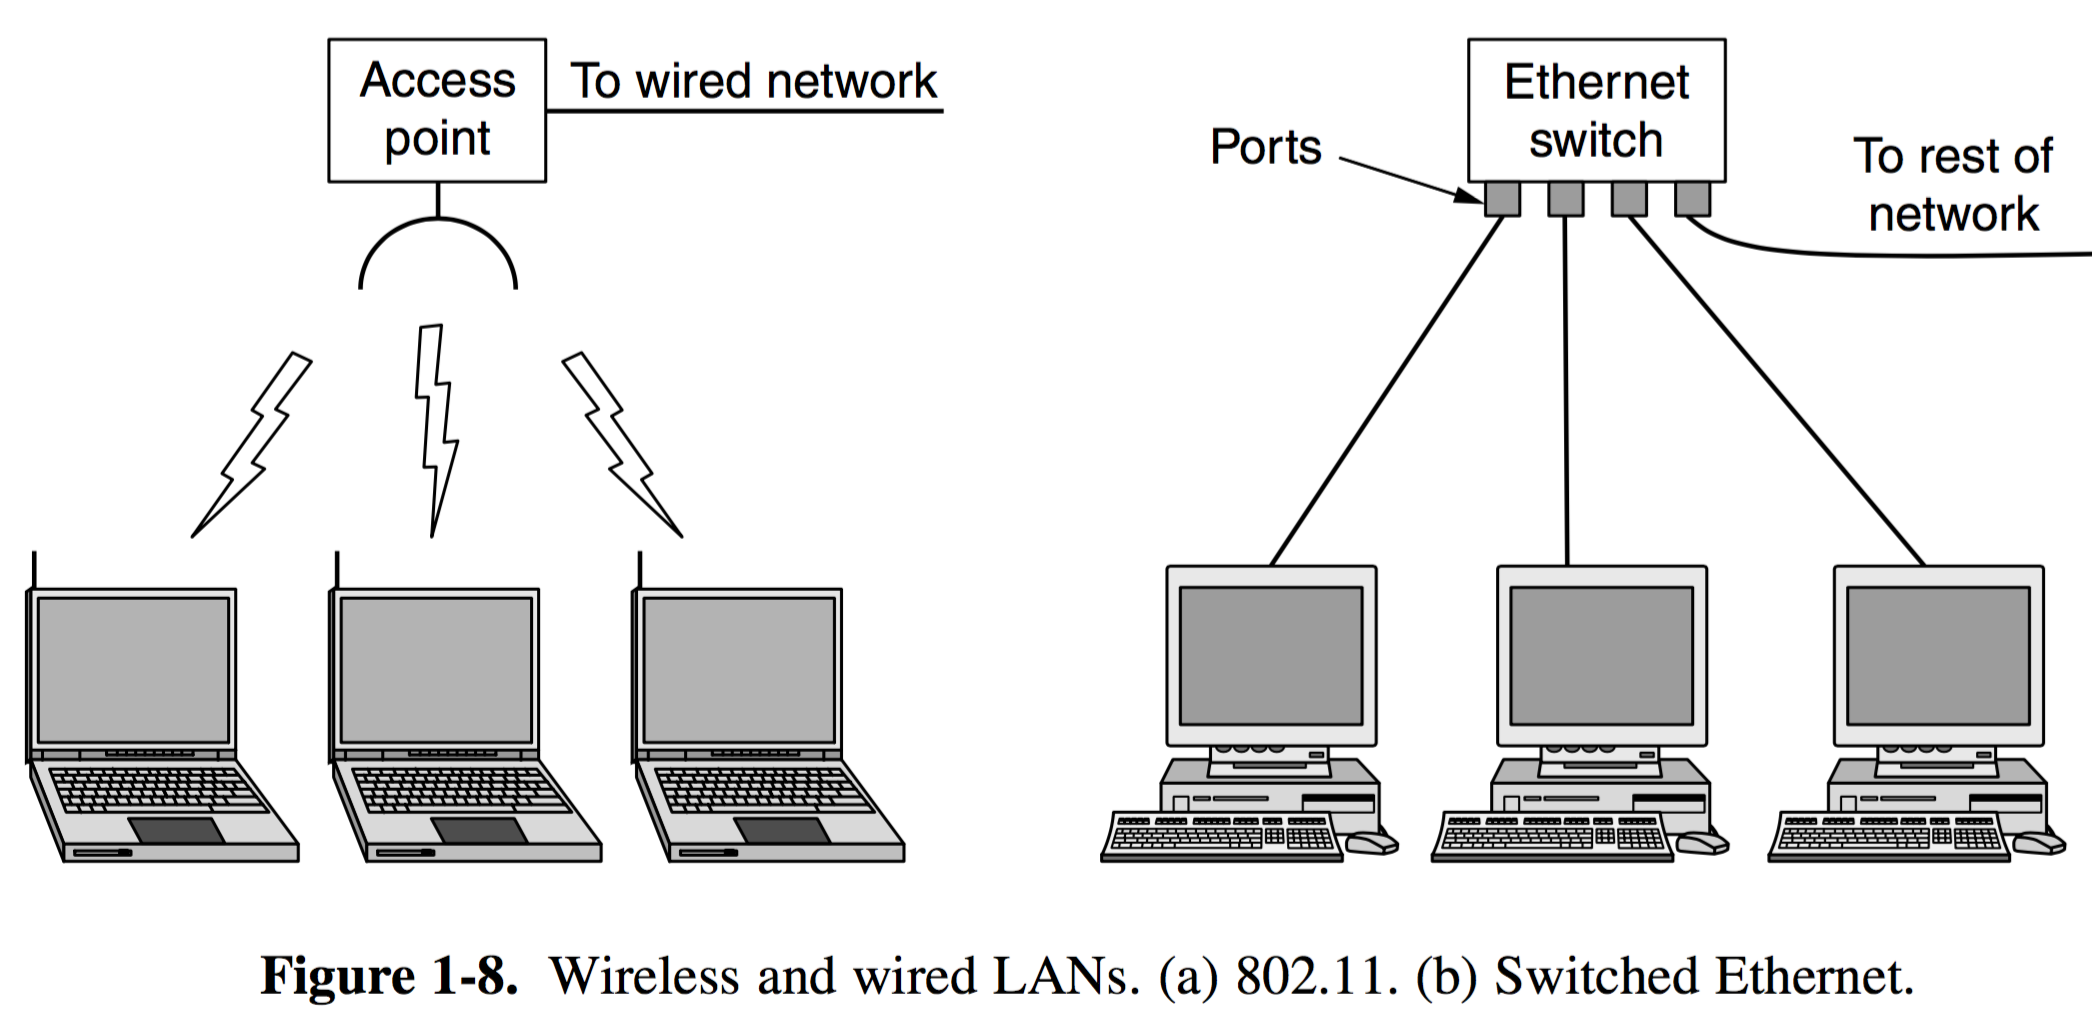
\includegraphics[width=8cm, height=6cm]{./imagenes/arealocal.png} 
\end{center}

\subsection{Redes de área metropolitana}
\par Una Red de área Metropolitana, o MAN (Metropolitan Area Network), cubre toda 
una ciudad.

\textbf{Ejemplo 1:} MAN basada en TV por cable
	\begin{itemize}
		\item Cable coaxil para unir varias casas.
		\item Elementos de conmutación.
		\item Elementos de conmuntación se unen por cables de fibra óptica.
	\end{itemize}
	
	\begin{center}
		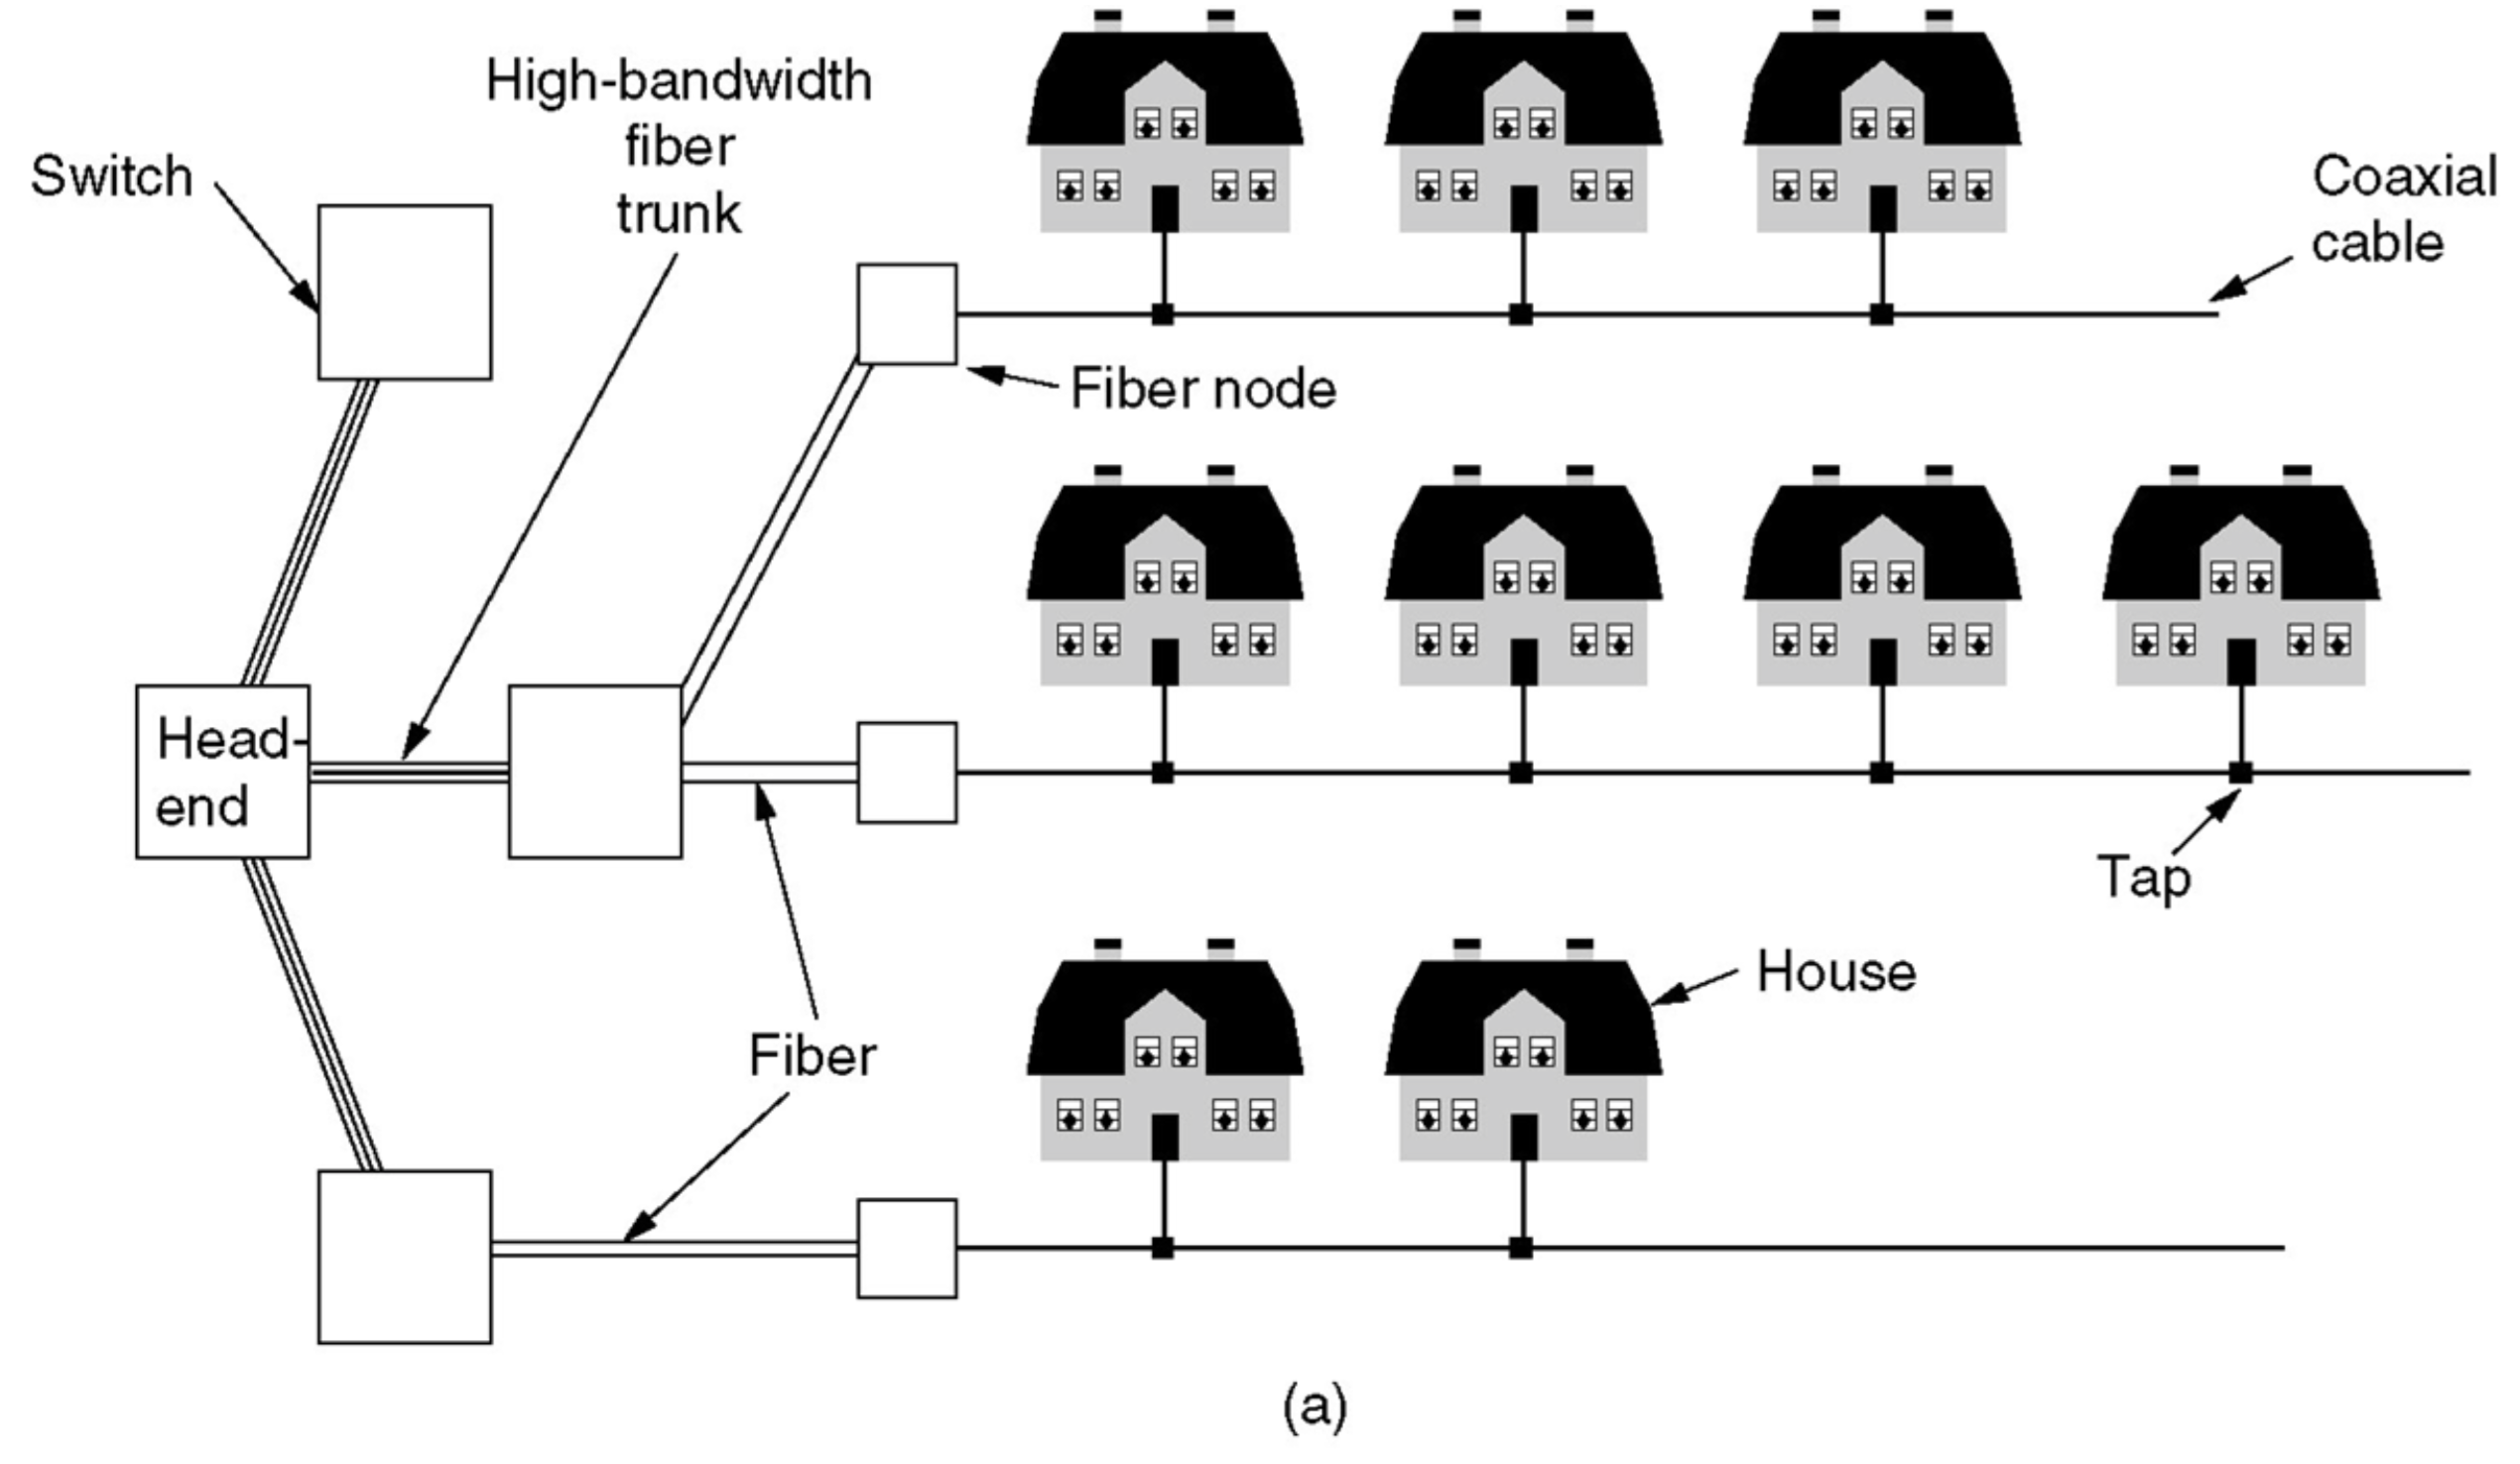
\includegraphics[width=10cm, height=6cm]{./imagenes/metropolitana1.png} 
	\end{center}

\textbf{Ejemplo 2:} Wimax (estándar 802.16).
	\begin{itemize}
		\item Se envían paquetes por el aire en lugar de usar cable o redes telefónicas.
		\item Se conecta a internet (a una red dorsal).
		\item Se puede acceder a la red desde computadoras en casas o edificios, o 
		desde vehículos en movimiento.
	\end{itemize}	 
	
	\begin{center}
		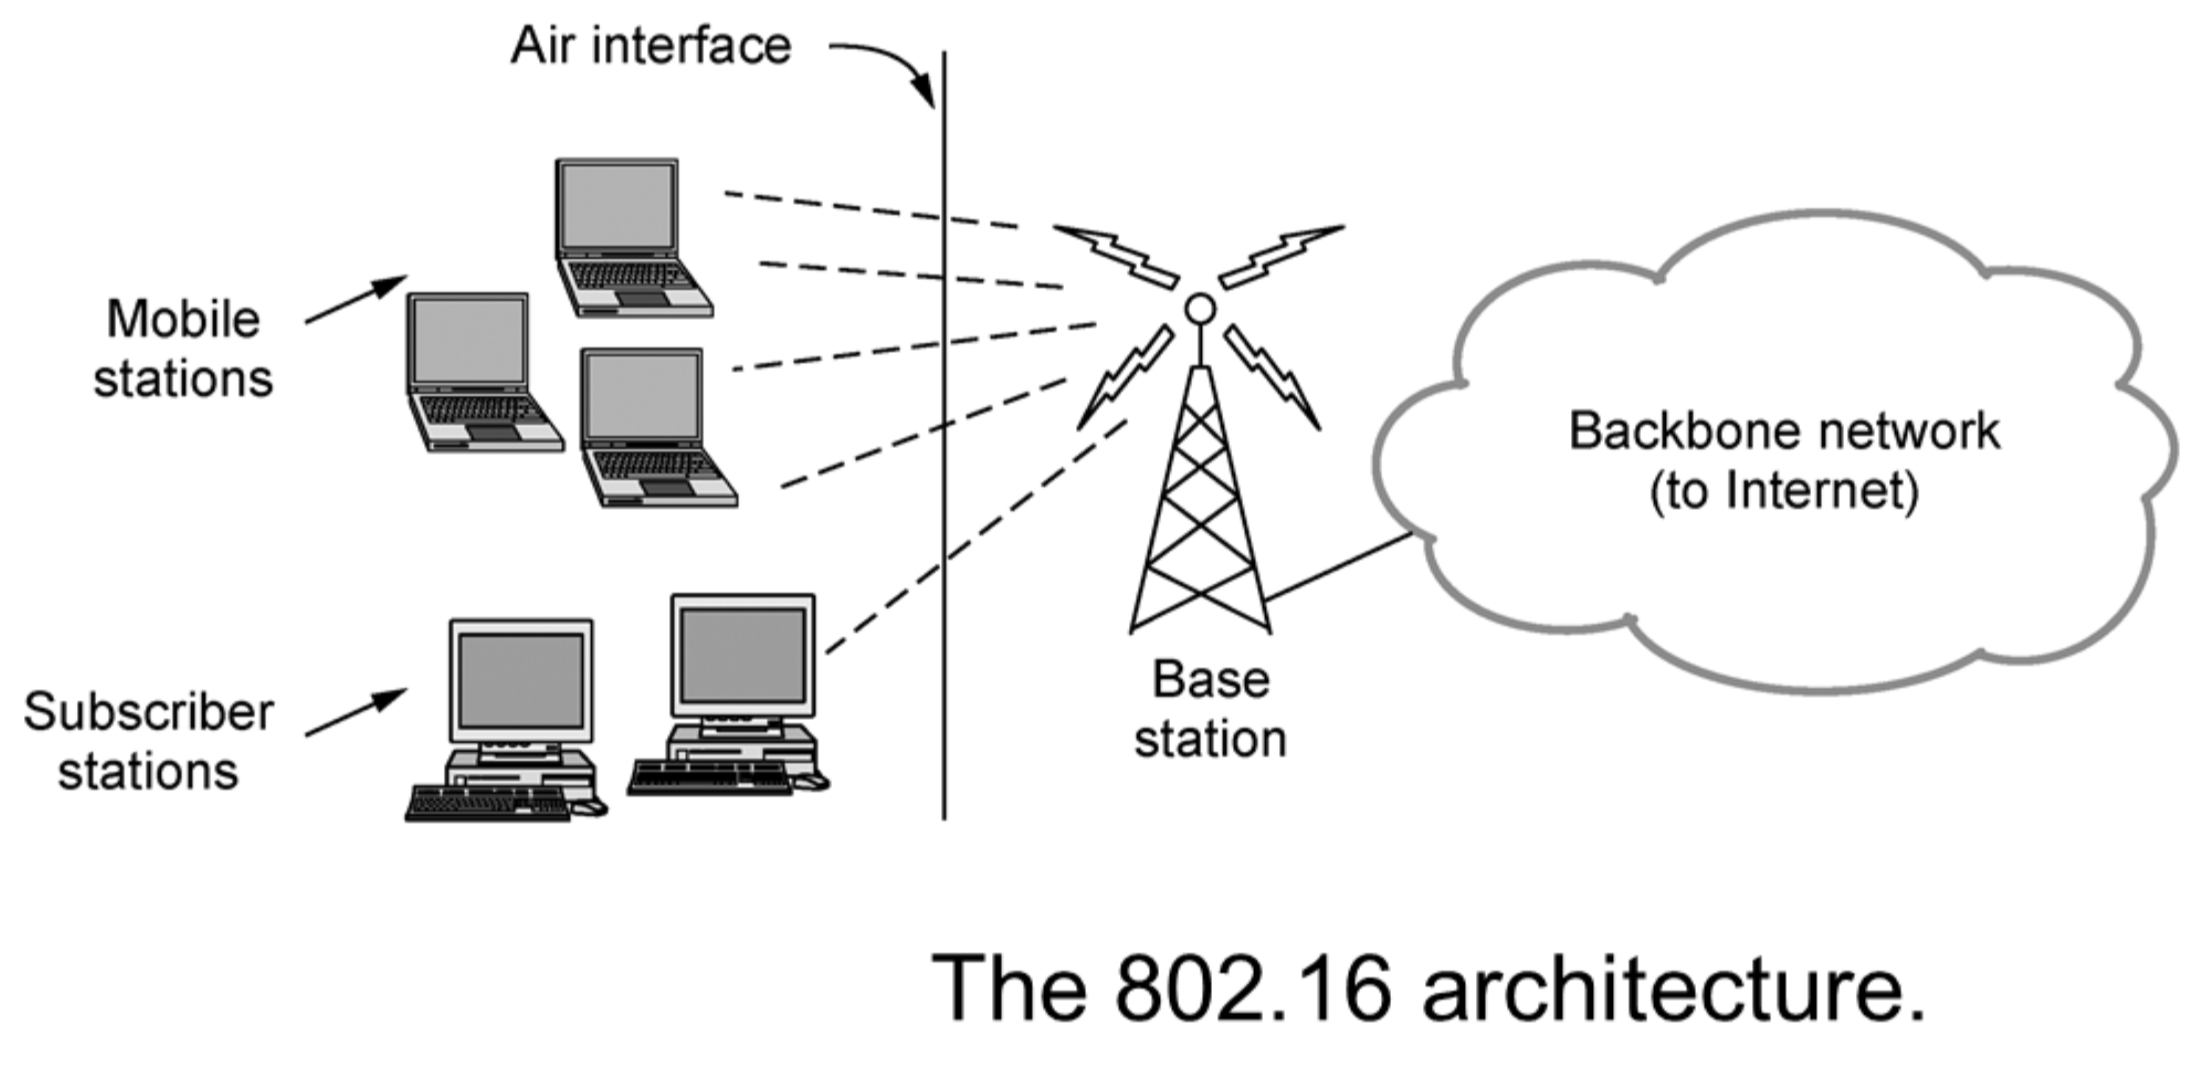
\includegraphics[width=10cm, height=6cm]{./imagenes/metropolitana2.png} 
	\end{center}

\subsection{Redes de área amplia}
\par Una Red de área Amplia, o WAN (Wide Area Network), abarca una extensa área 
geográfica, por lo general un país o continente. Son redes punto a punto: dos 
dispositivos están conectados entre sí por medio de un cable, esta regla da lugar a lo 
que se llama subred.
\par Una \textbf{subred} posee varios enrutadores conectados entre sí formando un 
grafo. A una subred pueden estar conectadas computadoras o redes de área local 
enteras, para ir de una máquina a otra hay distintas rutas alternativas.
\par Los elementos de conmutación, tambien llamados enrutadores dependiendo de la capa de red en la actúan, conectan tres o más líneas de transmisión. Los datos por línea de entrada se envían por alguna línea de salida elegida especialmente.
Dos enrutadores que no comparten una línea de transmisión se conectan indirectamente a través de otros enrutadores.

Un paquete se envía de un enrutador a otro a través de enrutadores intermedios, almacenándose enteramente en cada enrutador intermedio hasta que la línea requerida de salida esté libre y luego se reenvía (store-and-forward). Otra forma sería no guardar el mensaje, no esperar a que llegue entero antes de reenviarlo (cut-through).

Los mensajes se dividen en paquetes, los cuales tienen un número de secuencia. Estos paquetes se mandan en la red de uno en uno. Los paquetes se van depositando en el host receptor que reensambla el mensaje original. En algunas redes todos los paquetes del mensaje deben seguir la misma ruta, en otras cada paquete se enruta por separado. Las decisiones de enrutamiento se hacen de manera local, un algoritmo de enrutamiento describe la manera en que un enrutador toma esa decisión.

\subsubsection{Ejemplos de WAN:}
\begin{itemize}
\item Sistema telefónico fijo (Ej:. ADSL):
\begin{itemize}
	\item Cada domicilio conectado por un cable de cobre a una End office
 	\item Toll offices usadas para reenvío de mensajes.
 	\item Toll offices unidas por cables de fibra óptica llamados troncales.
\end{itemize}	

\begin{center} 
	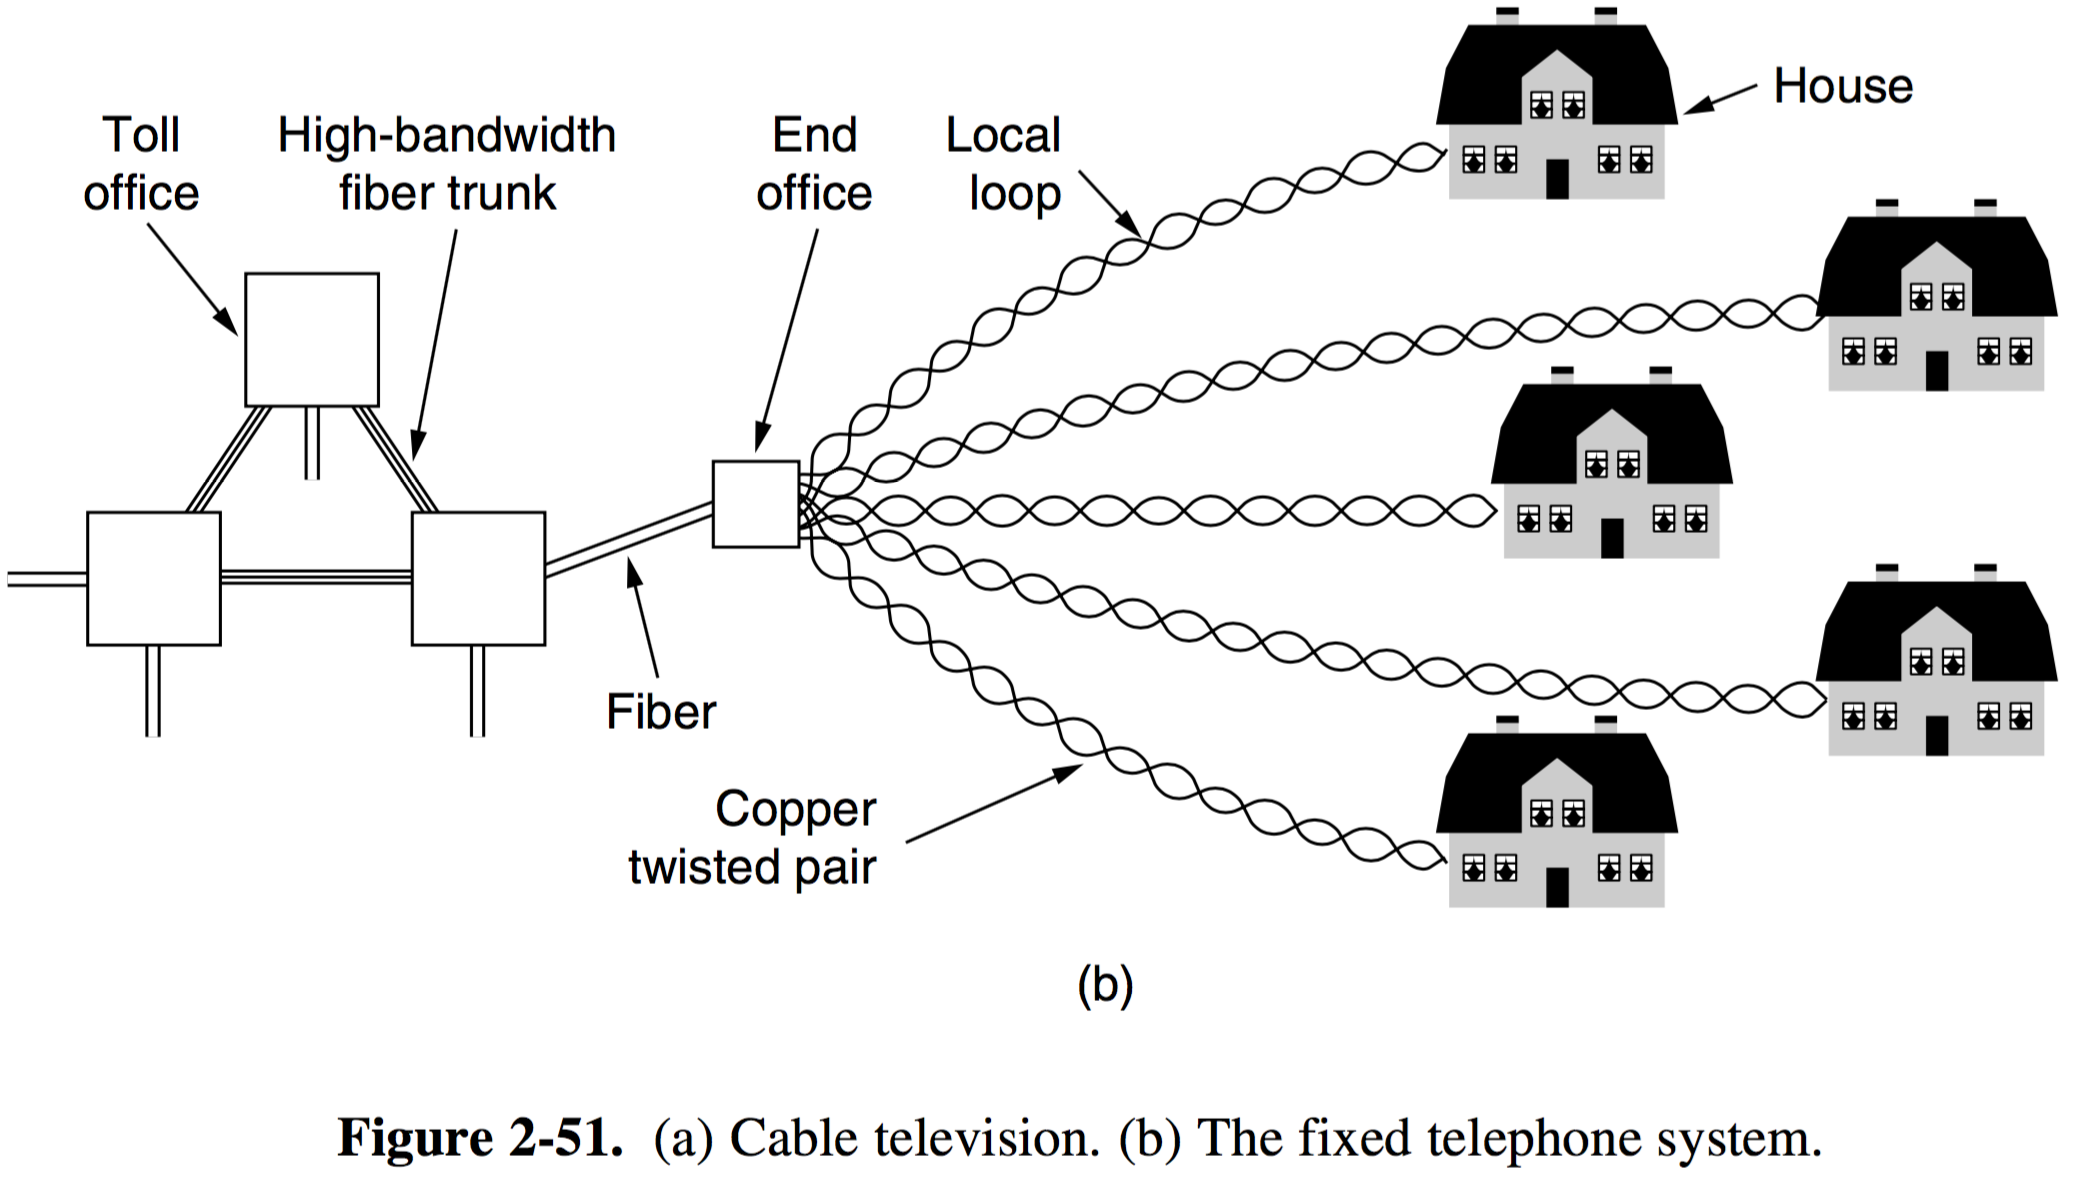
\includegraphics[width=8cm, height=6cm]{./imagenes/telefonico.png} 
\end{center}

\item Una red de teléfonos celulares (Ej: 3G o 4G).
\begin{itemize}
	\item Celdas con estaciones base: cada smartphone opera en una celda.
	\item Celdas conectados a centros de conmutación: para conectar distintas celdas
 	\item Centros de conmutación conectados a la red telefónica pública.
\end{itemize}

\end{itemize}

\par Un proveedor de servicios de internet (PSI) es también una WAN. Los clientes compran conectividad a un PSI y para usar su red.

\subsection{Interredes}
\par Existen mucha redes en el mundo, a veces con hardware y software diferente. 
Con frecuencia las personas conectadas a una red desean comunicarse con las 
personas conectadas a otra red diferente. Las puertas de enlace proveen la conexión y 
la traducción necesaria. Un conjunto de redes interconectadas se llama interred 
(internet), Internet es una inter red.

\begin{center} 
	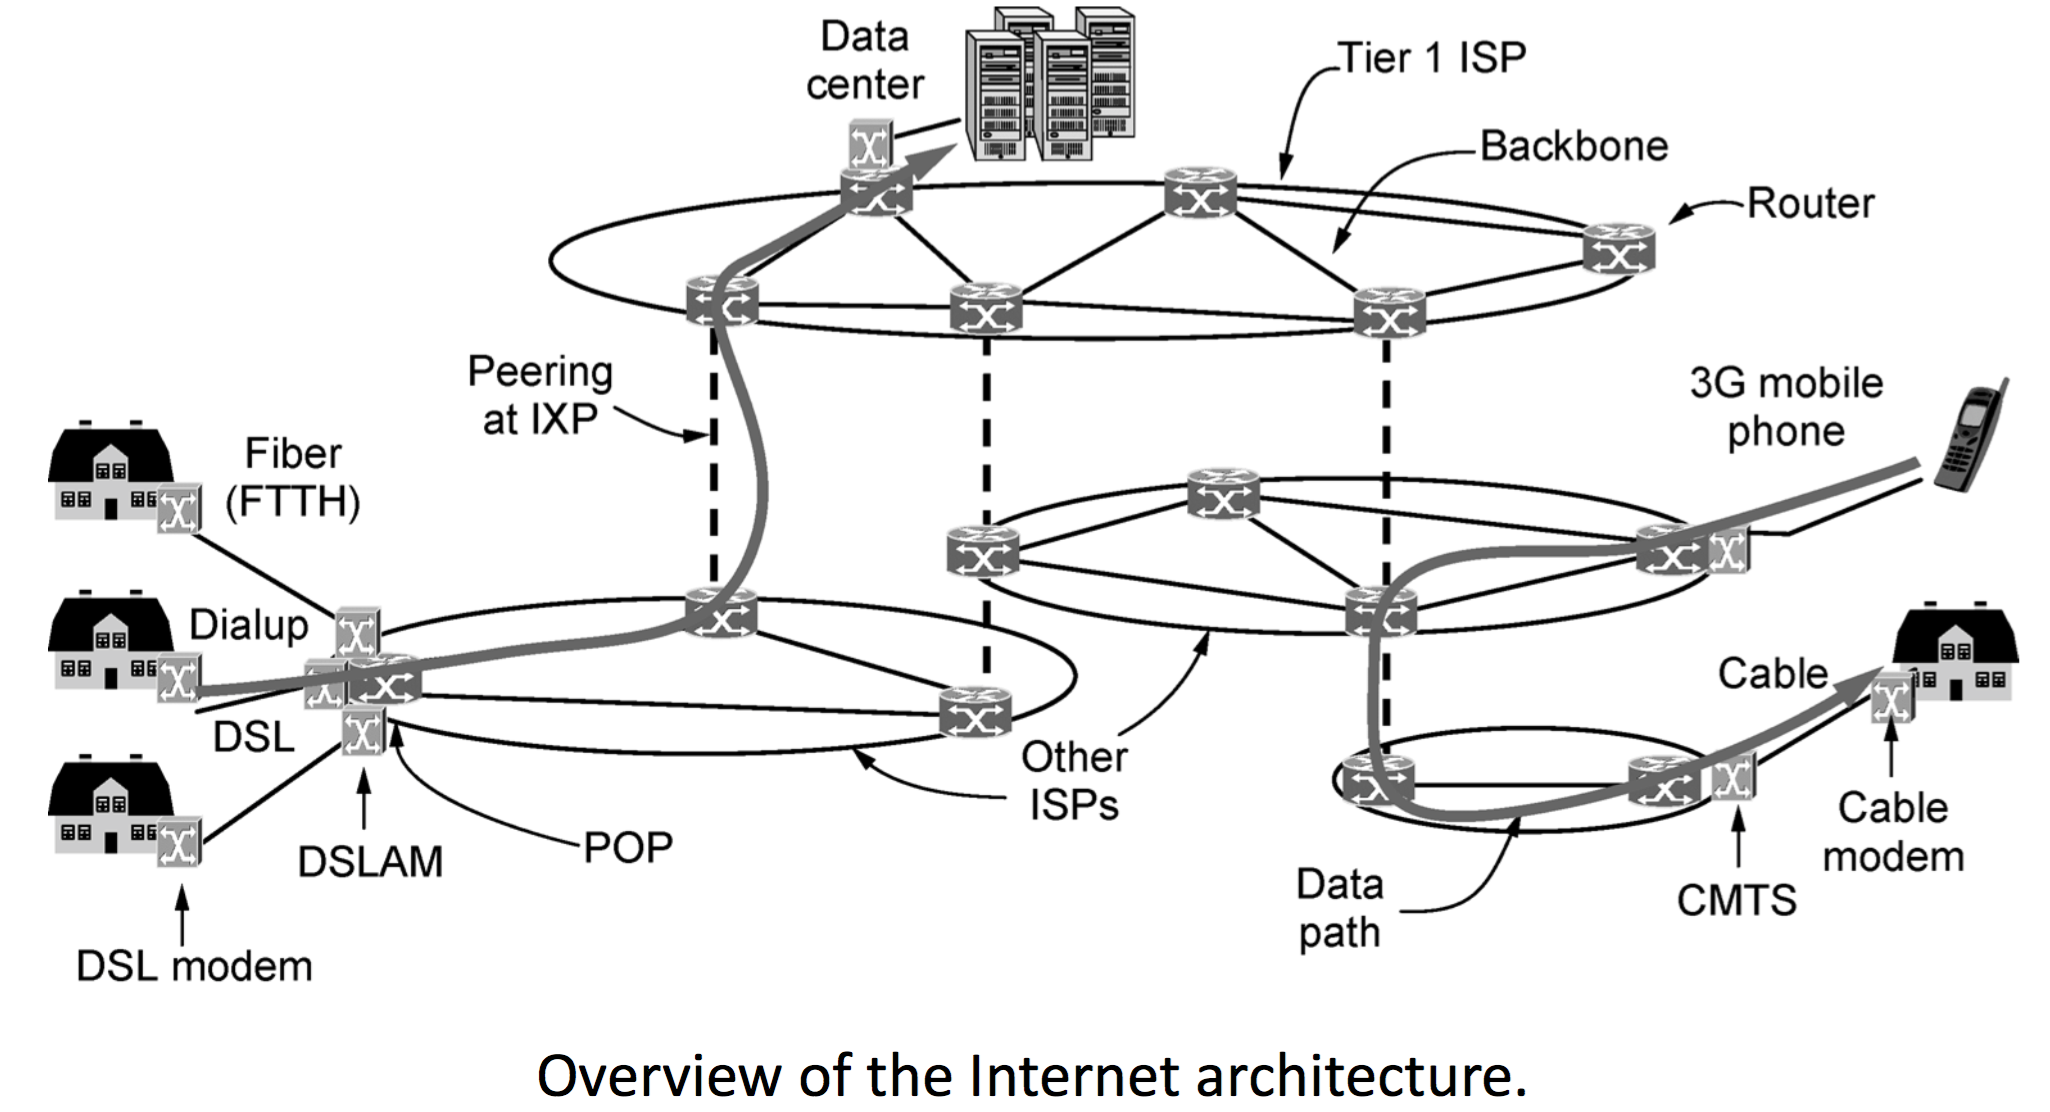
\includegraphics[width=8cm, height=6cm]{./imagenes/interred.png} 
\end{center}

\section{Software de red}
\par Las primeras redes de computadoras se diseñaron teniendo en cuenta al hardware 
como punto principal y al software como secundario. Pero esta estrategia ya no 
funciona. Ahora el software de red está muy estructurado.

\subsection{Jerarquías de protocolos}
\par Para reducir la complejidad de su diseño, la mayoría de las redes esta organizada 
como una pila de capas o niveles, cada una construida a partir de la que esta debajo de 
ella. El propósito de cada capa es ofrecer ciertos servicios, a las capas superiores, a las 
cuales no se les muestran los detalles de implementación de los servicios ofrecidos. La 
capa \textit{N} de una maquina mantiene una conversación con la capa \textit{N} de 
otra máquina. Las reglas y convenciones utilizadas en esta conversación se conocen 
como \textbf{protocolo de capa N}.
\par Cada capa pasa los datos y la información de control a la capa inmediatamente 
inferior, hasta que se alcanza la capa más baja. Debajo de la capa 1 se encuentra el 
medio físico, a través del cual ocurre la comunicación real. Entre cada par de capas 
adyacentes esta una \textbf{interfaz} que define que operaciones y servicios 
primitivos pone la capa mas baja a disposición de la capa superior inmediata.
\par El conjunto de capas y protocolos se conoce como \textbf{arquitectura de red} o 
\textbf{nomenclatura de pila de protocolos}.

\par Un proceso de aplicación se ejecuta en la \textit{capa 5}, la cual produce un 
mensaje y lo pasa a la \textit{capa 4} para su transmisión. La \textit{capa 4} pone un 
encabezado en el mensaje para identificarlo y pasa el resultado a la \textit{capa 3}. El 
encabezado contiene información de control como números de secuencia para que la 
\textit{capa 4} de la máquina de destino entregue los mensajes en el orden correcto, 
si las capas inferiores no mantienen la secuencia.

\par En muchas redes no hay limitaciones en el tamaño de los mensajes de la 
\textit{capa 4}, pero casi siempre hay un límite impuesto por el protocolo de la 
\textit{capa 3}, la cual debe dividir  los mensajes que llegan en unidades mas 
pequeñas llamadas \textbf{paquetes} y a cada paquete colocarle un encabezado.
\par La \textit{capa 3} decide cuál de las líneas que salen utilizar y pasa los paquetes 
a la \textit{capa 2} que no solo agrega un encabezado a cada pieza sino tambien un 
terminador, y pasa la unidad resultante a la \textit{capa 1} para su transmisión.
\par En la máquina receptora el mensaje pasa hacia arriba de capa en capa, perdiendo 
los encabezados conforme avanza.

\subsection{Aspectos de diseño para las capas}

Algunos de los aspectos claves de diseño que ocurren en la redes están presentes en 
las diversas capas, cada capa necesita de un mecanismo para identificar a los emisores 
y a los receptores. Es necesario un método para que un proceso en una máquina 
especifique con cual otra máquina quiere hablar, además de una forma de 
\textbf{direccionamiento} a fin de precisar un destino específico.

\par Otras decisiones de diseño conciernen a las reglas de transferencia de datos, en 
algunos sistemas los datos viajan solo en una dirección, en otros pueden viajar en 
ambas direcciones.

El control de errores es un aspecto importante porque los circuitos de comunicación 
física no son perfectos. Muchos códigos de corrección y detección de errores son 
conocidos, pero los dos extremos de la conexión deben estar de acuerdo en cual es el 
que se va a utilizar. Además, el receptor debe tener algun medio de decirle al emisor 
que mensajes se han recibido correctamente y cuáles no.

\par No todos los canales de comunicación conservan el orden en que se envían los 
mensajes. Para tratar con una posible perdida de secuencia, el protocolo debe incluir 
un mecanismo que permita al receptor volver a unir los pedazos en forma adecuada. 
Una solución obvia es numerar las piezas, pero hay que tratar con las piezas que no 
llegan en orden.

\par Hay que evitar que un emisor rápido sature de datos a un receptor lento. Hay 
soluciones a este problema donde el receptor proporciona algún tipo de 
retroalimentación al emisor, directa o indirectamente, dependiendo de la situación real 
del receptor. A este tema se lo denomina c\textbf{control de flujo}. A veces en la red 
demasiadas máquinas quieren enviar demasiados mensajes y la red no puede 
mandarlos a todos, esta sobrecarga se llama \textbf{congestión}. Una solución es que 
cada máquina emisora reduzca el tráfico de salida.

\par En algunos niveles los procesos son incapaces de aceptar mensajes de longitud 
arbitraria. Esta propiedad conduce a mecanismos para desensamblar, transmitir y 
reensamblar mensajes. A este tema en general se lo conoce como 
\textbf{interconexión de redes}.

\par Cuando es costoso mantener una conexión separada para cada par de procesos 
de comunicación, la capa subyacente podría decidir usar la misma conexión para 
múltiples conversaciones sin relación entre si, siempre y cuando esta 
\textbf{multiplexión} y demultiplexión se realice de manera transparente, cualquier 
capa la podrá utilizar. La multiplexión se necesita en la capa física, donde múltiples 
conversaciones comparten un número limitado de circuitos físicos.

\par Cuando hay múltiples rutas entre el origen y el destino se debe elegir la mejor o 
las mejores entre todas ellas, este tema se llama \textbf{enrutamiento}.

\subsection{Comparación entre servicio orientado a conexión y servicio sin conexión}
\par Normalmente una capa puede ofrecer distintos tipos de servicio a las capas arriba 
suyo. El servicio orientado a la conexión, el usuario del servicio primero establece una 
conexión, la utiliza y luego la abandona. Una conexión funciona como un tubo: el 
emisor empuja objetos en un extremo y el receptor los toma en el otro extremo. Se 
conserva el orden en que esos objetos salen y llegan.
\par En el servicio no orientado a la conexión cada mensaje lleva completa la dirección 
de destino y cada uno se enruta a través del sistema, independientemente de los 
demás. Algunos servicios son confiables en el sentido que nunca pierden datos, pero 
por lo general en un servicio confiable el receptor confirma la recepción de cada 
mensaje. Al servicio no orientado a la conexión no confiable, es decir sin confirmación 
de recepción, se lo conoce como servicio de datagramas. 
\par A veces se desea no tener que establecer una conexión para enviar un mensaje 
corto, pero la confiabilidad es esencial. Para estas aplicaciones se usa el servicio de 
\textbf{datagramas confirmados}. En el servicio de \textbf{solicitud-respuesta} el 
emisor transmite un solo datagrama con una solicitud y luego el receptor envía la 
respuesta al estilo del modelo cliente-servidor.


\section{Modelos de referencia}

\subsection{El modelo de referencia OSI}

\subsubsection{La capa de enlace de datos}
\par La tarea principal de la capa de enlace de datos es transformar un medio de 
transmisión puro en una línea de comunicación que aparezca libre de errores de 
transmisión. El emisor fragmenta los datos de entrada en \textbf{tramas de datos}, y 
transmite las tramas de manera secuencial. Si el servicio es confiable, el receptor 
confirma la recepción correcta de cada trama devolviendo una \textbf{trama de 
confirmación de recepción}.
\par Otro problema atacado es como hacer que un emisor rápido no sature de datos a 
un receptor lento: mecanismo de regulación de tráfico. Con frecuencia esta regulación 
de flujo y el manejo de errores están integrados. Las redes de difusión además 
consideran como controlar el acceso a un canal compartido. La subcapa de control de 
acceso al medio se ocupa de esto.

\subsubsection{La capa de red}
\par La capa de red controla las operaciones de la subred. Hay que determinar cómo se enrutan los paquetes desde su origen a su destino. Si hay demasiados paquetes en la subred al mismo tiempo, se interpondrán en el camino unos y otros lo que hará que se formen cuellos de botella, la capa de red se ocupa de controlar esta congestión.
\par Cuando un paquete tiene que viajar de una red a otra para llegar a destino pueden surgir varios problemas; el direccionamiento de la segunda red podría ser distinto, la segunda podría no aceptar el paquete porque es demasiado largo, los protocolos podrían ser distintos, etc. La capa de red resuelve estos problemas.

\subsection{El modelo de referencia TCP/IP}

Se eligió una red de conmutación de paquetes basada en una capa de interred no 
orientada a la conexión.
– El trabajo de la capa de interred es permitir que los hosts inyecten paquetes dentro de cualquier red y que estos viajen a su destino de manera independiente.
– Tal vez lleguen en un orden distinto al cual fueron enviados, en cuyo caso las capas mas altas deberán ordenarlos, si se desea una entrega ordenada.
– La capa de interred define un paquete de formato y protocolo oficial llamado IP (protocolo de internet).
– Direcciones IP
• 4 números entre 0 y 255 separados por ‘.’ .
• P. ej. 200, 45.191.35
• El trabajo de la capa de interred es entregar paquetes IP al destinatario.
– El enrutamiento de paquetes es el aspecto principal, con el propósito de evitar la congestión.

 La capa arriba de la capa interred es la capa de transporte, la cual esta diseñada para permitir que las entidades iguales en los hosts de origen y destino puedan llevar a cabo una conversación.
 Se tienenn dos protocoles de transporte
– TCP es confiable, orientado a la conexión y permite que un flujo de bytes que se origina en una máquina se entregue sin errores en cualquier otra máquina en la interred.
 TCP divide el flujo en de bytes entrantes en mensajes discretos y pasa cada uno de ellos a la capa de interred.
 En el destino el proceso TCP receptor reensambla en el flujo de salida los mensajes recibidos.
 TCP también maneja el control de flujo para que un emisor rápido no sature con mas mensajes que los que puede manejar a un receptor lento.
– UDP es un protocolo no confiable y no orientado a la conexión, para aplicaciones que no desean el control de flujo ni la secuenciación de mensajes.
 Tiene un amplio uso en consultas de solicitud-respuesta de tipo cliente-servidor en un solo envío y en aplicaciones de transmisión de voz y video.

La capa de aplicación contiene todos los protocolos de nivel mas alto: terminal virtual (TELNET), transferencia de archivos (FTP), correo electrónico (SMTP), para resolución de nombres de host en sus direcciones de red (DNS), para páginas web (HTTP).

\subsection{Una crítica al modelo de referencia TCP/IP}

Problemas:
– No se distingue entre servicio, interfaz y protocolo.
 O sea no se distingue bien entre especificación e implementación.
– No es un modelo general: no esta ajustado para describir ninguna pila de protocolos mas que TCP/IP.
– No se mencionan las capas físicas y de enlace de datos
– Protocolos altamente entrincherados y difíciles de remplazar.

\section{Redes de ejemplo}

\subsection{Internet}
\par Internet es un inmenso conjunto de redes diferentes, que usan ciertos 
protocolos comunes y proporcionan ciertos servicios comunes. A este sistema nadie 
lo planeo y nadie lo controla. 
\par Los protocolos TCP e IP están preparados para manejar comunicaciones por 
interredes. Se desarrollo una interfaz de programación para la red llamada sockets 
de Berkley.

– Luego se creo el DNS (sistema de nombres de dominios) para organizar máquinas 
dentro de dominios y resolver nombres de hosts en direcciones IP.
– Una máquina esta en Internet si ejecuta una pila de protocolos TCP/IP, tiene una 
dirección IP y puede enviar paquetes a todas las demás maquinas de Internet.

Muchas máquinas pueden llamar a un proveedor de servicios de Internet mediante 
un modem, recibir direcciones IP temporales y enviar paquetes a otros hosts de 
Internet.

\subsection{El modelo utilizado en este libro}
\section{Resumen}

\par Las redes de computadoras tienen muchos usos, tanto para empresas como para 
individuos, en el hogar y en movimiento. Las empresas usan redes de computadoras 
para compartir la información corporativa, por lo general mediante el modelo cliente-
servidor en donde las computadoras de los empleados actúan como clientes que 
acceden a poderosos servidores en la sala de máquinas. Para los individuos, las redes 
ofrecen acceso a una variedad de recursos de información y entretenimiento, así como 
una manera de comprar y vender productos y servicios. Con frecuencia los individuos 
acceden a Internet por medio de sus proveedores de teléfono o cable en el hogar, 
aunque cada vez se utiliza más el acceso inalámbrico para laptops y teléfonos. Los 
avances tecnológicos permiten nuevos tipos de aplicaciones móviles y redes con 
computadoras integradas a los electrodomésticos y demás dispositivos para el 
consumidor. Los mismos avances generan cuestiones sociales tales como las 
relacionadas con la privacidad.
\par En términos generales, podemos dividir a las redes en LAN, MAN, WAN e 
interredes. Por lo general las redes LAN cubren todo un edificio y operan a velocidades 
altas. Las redes MAN comúnmente cubren toda una ciudad. El sistema de televisión 
por cable es un ejemplo, ya que ahora muchas personas lo utilizan para acceder a 
Internet. Las redes WAN pueden cubrir un país o continente. Algunas de las 
tecnologías utilizadas para construir estas redes son de punto a punto (como un 
cable), mientras que otras son de difusión (como las redes inalámbricas). Las redes se 
pueden interconectar con enrutadores para formar interredes, de las cuales Internet es 
el ejemplo más grande y popular. Las redes inalámbricas, como las redes LAN 802.11 
y de telefonía móvil 3G, también se están volviendo muy populares.
\par El software de red se basa en los protocolos, que son reglas mediante las cuales 
los procesos se comunican entre sí. La mayoría de las redes soportan jerarquías de 
protocolos, en donde cada capa proporciona servicios a la capa inmediata superior y 
los aísla de los detalles sobre los protocolos que se utilizan en las capas inferiores. Por 
lo general las pilas de protocolos se basan en el modelo OSI o en el modelo TCP/IP. 
Ambos modelos tienen capas de enlace, red, transporte y aplicación, pero difieren en 
las otras capas. Los aspectos de diseño incluyen: confiabilidad, asignación de recursos, 
crecimiento, seguridad, etc.
\par Las redes proveen varios servicios a sus usuarios. Estos servicios pueden variar, 
desde la entrega de paquetes sin conexión de mejor esfuerzo hasta la entrega 
garantizada orientada a conexión. En algunas redes se proporciona servicio sin 
conexión en una capa y servicio orientado a conexión en la capa inmediata superior.
Entre las redes más conocidas están: Internet, la red de telefonía móvil 3G y las redes 
LAN 802.11. Internet evolucionó de ARPANET, a la que se agregaron otras redes para 
formar una interred. En realidad la Internet de la actualidad es una colección de 
muchos miles de redes que utilizan la pila de protocolos TCP/IP. La red de telefonía 
móvil 3G proporciona acceso inalámbrico y móvil a Internet, con es LAN inalámbricas 
basadas en el estándar IEEE 802.11 se implementan en muchos hogares y cafés; 
pueden proporcionar conectividad a velocidades en mayores 100 Mbps. También están 
surgiendo nuevos tipos de redes, como las redes de sensores integradas y las redes 
basadas en tecnología RFID.
Para permitir que varias computadoras se comuniquen entre sí se requiere una gran 
cantidad de estandarización, tanto en hardware como en software. Las organizaciones 
tales como ITU-T, ISO, IEEE e IAB administran distintas partes del proceso de 
estandarización.




\chapter{LA CAPA DE RED}
La capa de red se encarga de llevar los paquetes todo el camino, desde el origen hasta el destino. Para llegar al destino tal vez sea necesario realizar muchos saltos en el camino por enrutadores intermedios. Esta función ciertamente contrasta con la de la capa de enlace de datos, cuya única meta es mover tramas de un extremo del cable al otro. Por lo tanto, la capa de red es la capa más baja que maneja la transmisión de extremo a extremo.
\par Para lograr sus objetivos, la capa de red debe conocer la topología de la red (es
decir, el conjunto de todos los enrutadores y enlaces) y elegir las rutas apropiadas
incluso para redes más grandes. También debe tener cuidado al escoger las rutas para
no sobrecargar algunas de las líneas de comunicación y los enrutadores, y dejar
inactivos a otros. Por último, cuando el origen y el destino están en redes diferentes, ocurren nuevos problemas. La capa de red es la encargada de solucionarlos. En este capítulo estudiaremos todos estos temas y los ilustraremos, principalmente mediante el uso de Internet y su protocolo de capa de red, IP.

\section{Aspectos de diseño de la capa de red}
\subsection{Servicios proporcionados a la capa de transporte}

La capa de red proporciona servicios a la capa de transporte en la interfaz entre la 
capa de red y de transporte. Una pregunta importante es qué tipo de servicios 
proporciona precisamente la capa de red a la capa de transporte. Hay que diseñar los 
servicios de manera cuidadosa, con los siguientes objetivos en mente:
	\begin{itemize}
		\item Los servicios deben ser independientes de la tecnologia del 			
		enrutador.
		\item La capa de transporte debe estar aislada de la cantidad, tipo y topología 
		de los enrutadores presentes.
		\item Las direcciones de red disponibles para la capa de transporte deben usar 
		un plan de numeracin uniforme, incluso a traves de redes LAN y WAN.
	\end{itemize}
\par Dadas estas metas, los diseñadores de la capa de red tienen mucha libertad para 
escribir especificaciones detalladas de los servicios que se ofrecerán a la capa de 
transporte. Con frecuencia esta libertad degenera en una batalla campal entre dos 
bandos en conflicto. La discusión se centra en determinar si la capa de red debe 
proporcionar un servicio orientado a conexión o un servicio sin conexión.
\par Estos dos bandos son:
	\begin{enumerate}
		\item La comunidad de internet
		\begin{itemize}\itemsep=0pt
			\item La tarea del enrutador es solo mover bits de un lado a otro.
			\item La subred es inherentemente inestable. Los hosts deben efectuar el 
			control de errores y el control de flujo.
			\item No debe efectuarse ningún ordenamiento de paquetes.
			\item Cada paquete se transportará de manera independiente a sus 
			antecesores.
			\end{itemize}
		\item Las compañías telefónicas:
		\begin{itemize}\itemsep=0pt
			\item La subred debe proporcionar un servicio confiable, orientado a la
conexión..
			\item La subred es inherentemente inestable. Los hosts deben efectuar el 
			control de errores y el control de flujo.
			\item La calidad del servicio es el factor dominante, sin conexiones en la 
			subred tal calidad es muy difícil de alcanzar, especialmente para el tráfico de 
			tiempo real como la voz y el video.
		\end{itemize}
	\end{enumerate}
\par Los dos bandos se ejemplifican con Internet y las redes ATM.

\subsection{Implementación del servicio sin conexión}
	\begin{itemize}\itemsep=0pt
			\item Los paquetes se colocan individualmente en la subred y se enrutan de
manera independiente.  Por eso debe levar una dirección de destino completa. 
			\item \textbf{Datagramas} = paquetes
			\item \textbf{Subred de Datagramas} = subred
			\item Tabla interna de un enrutador
			\par Entrada de la tabla interna = (destino, línea de salida)
			\par Cuando llega un paquete: Se lo almacena y se comprueba que llegó bien; se reenvía al destino de acuerdo con la tabla del enrutador.
			\item Los enrutadores requieren la capacidad de reemplazar identificadores de conexión en los paquetes salientes, ya que podria darse el caso de que un host H1 inicie una conexión con identificador 1; luego otro host H3 inicia conexión con identificador 1, y ambos hosts están conectados al mismo enrutador A.
			\end{itemize}
	\par Ahora veamos como funciona una red de datagramas. Suponga que el proceso P1 de la figura tiene un mensaje largo para P2. Dicho proceso entrega el mensaje a la capa de transporte y le indica a ésta que lo envíe al proceso P2 en el host H2. El código de la capa de transporte se ejecuta en H1, por lo general dentro del sistema operativo. Dicho código agrega un encabezado de transporte al frente del mensaje y entrega el resultado a la capa de red, que quizá sólo sea otro procedimiento dentro del sistema operativo.
\begin{center} 
	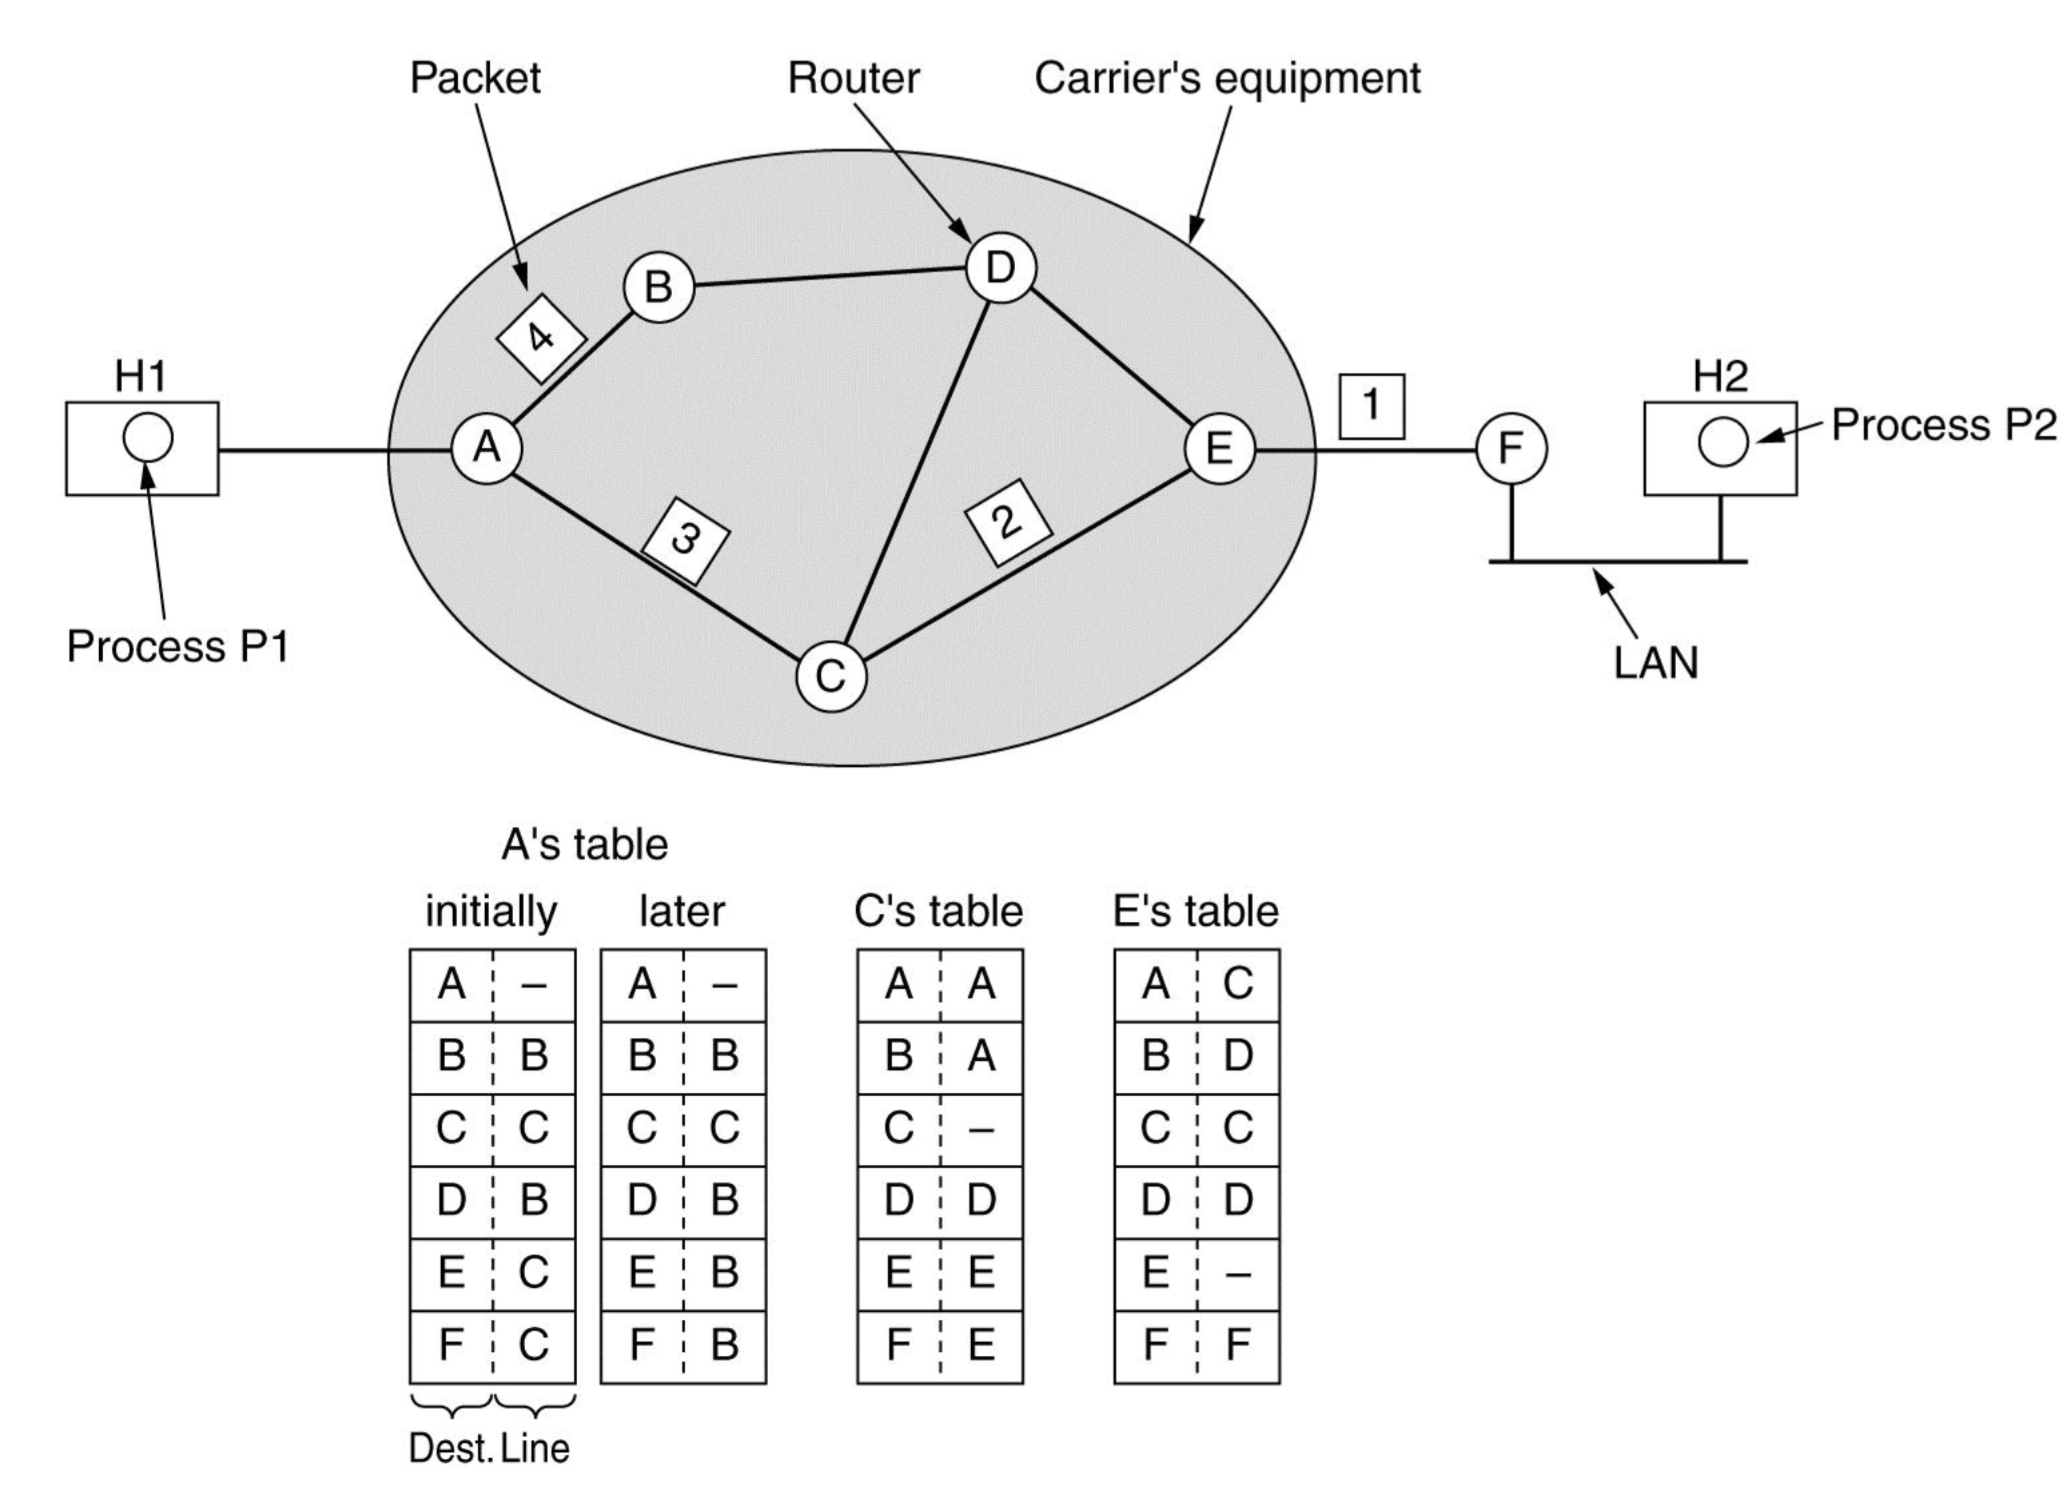
\includegraphics[width=8cm, height=6cm]{./imagenes/norientado.png} 
\end{center}

\par Problema:  
\par IP es el ejemplo dominante de un servicio de red sin conexión. Cada paquete 
transporta una dirección IP de destino que los enrutadores usan para reenviar cada 
paquete por separado. Las direcciones son de 32 bits en los paquetes IPv4 y de 128 
bits en los paquetes IPv6.

\subsection{Implementación del servicio orientado a conexión}
	\begin{itemize}\itemsep=0pt
			\item \textbf{Conexiónes o circuitos virtuales (CV)}
			\item \textbf{Subred de Circuitos Virtuales} = subred
			\item Evitar la necesidad de elegir una nueva ruta para cada paquete enviado. 
			La ruta de una conexión se almacena en tablas en los enrutadores, esta ruta se 
			usa para todo el tráfico que fluye a través de la conexión.
			\item Cada paquete lleva un identificador de CV.
			\item Liberación de conexión: se termina el CV
			\item Se paga el precios del espacio de tabla en los enrutadores. El uso de CVs 
			requiere una fase de configuración que consume tiempo y recursos.
	\end{itemize}

\begin{center} 
	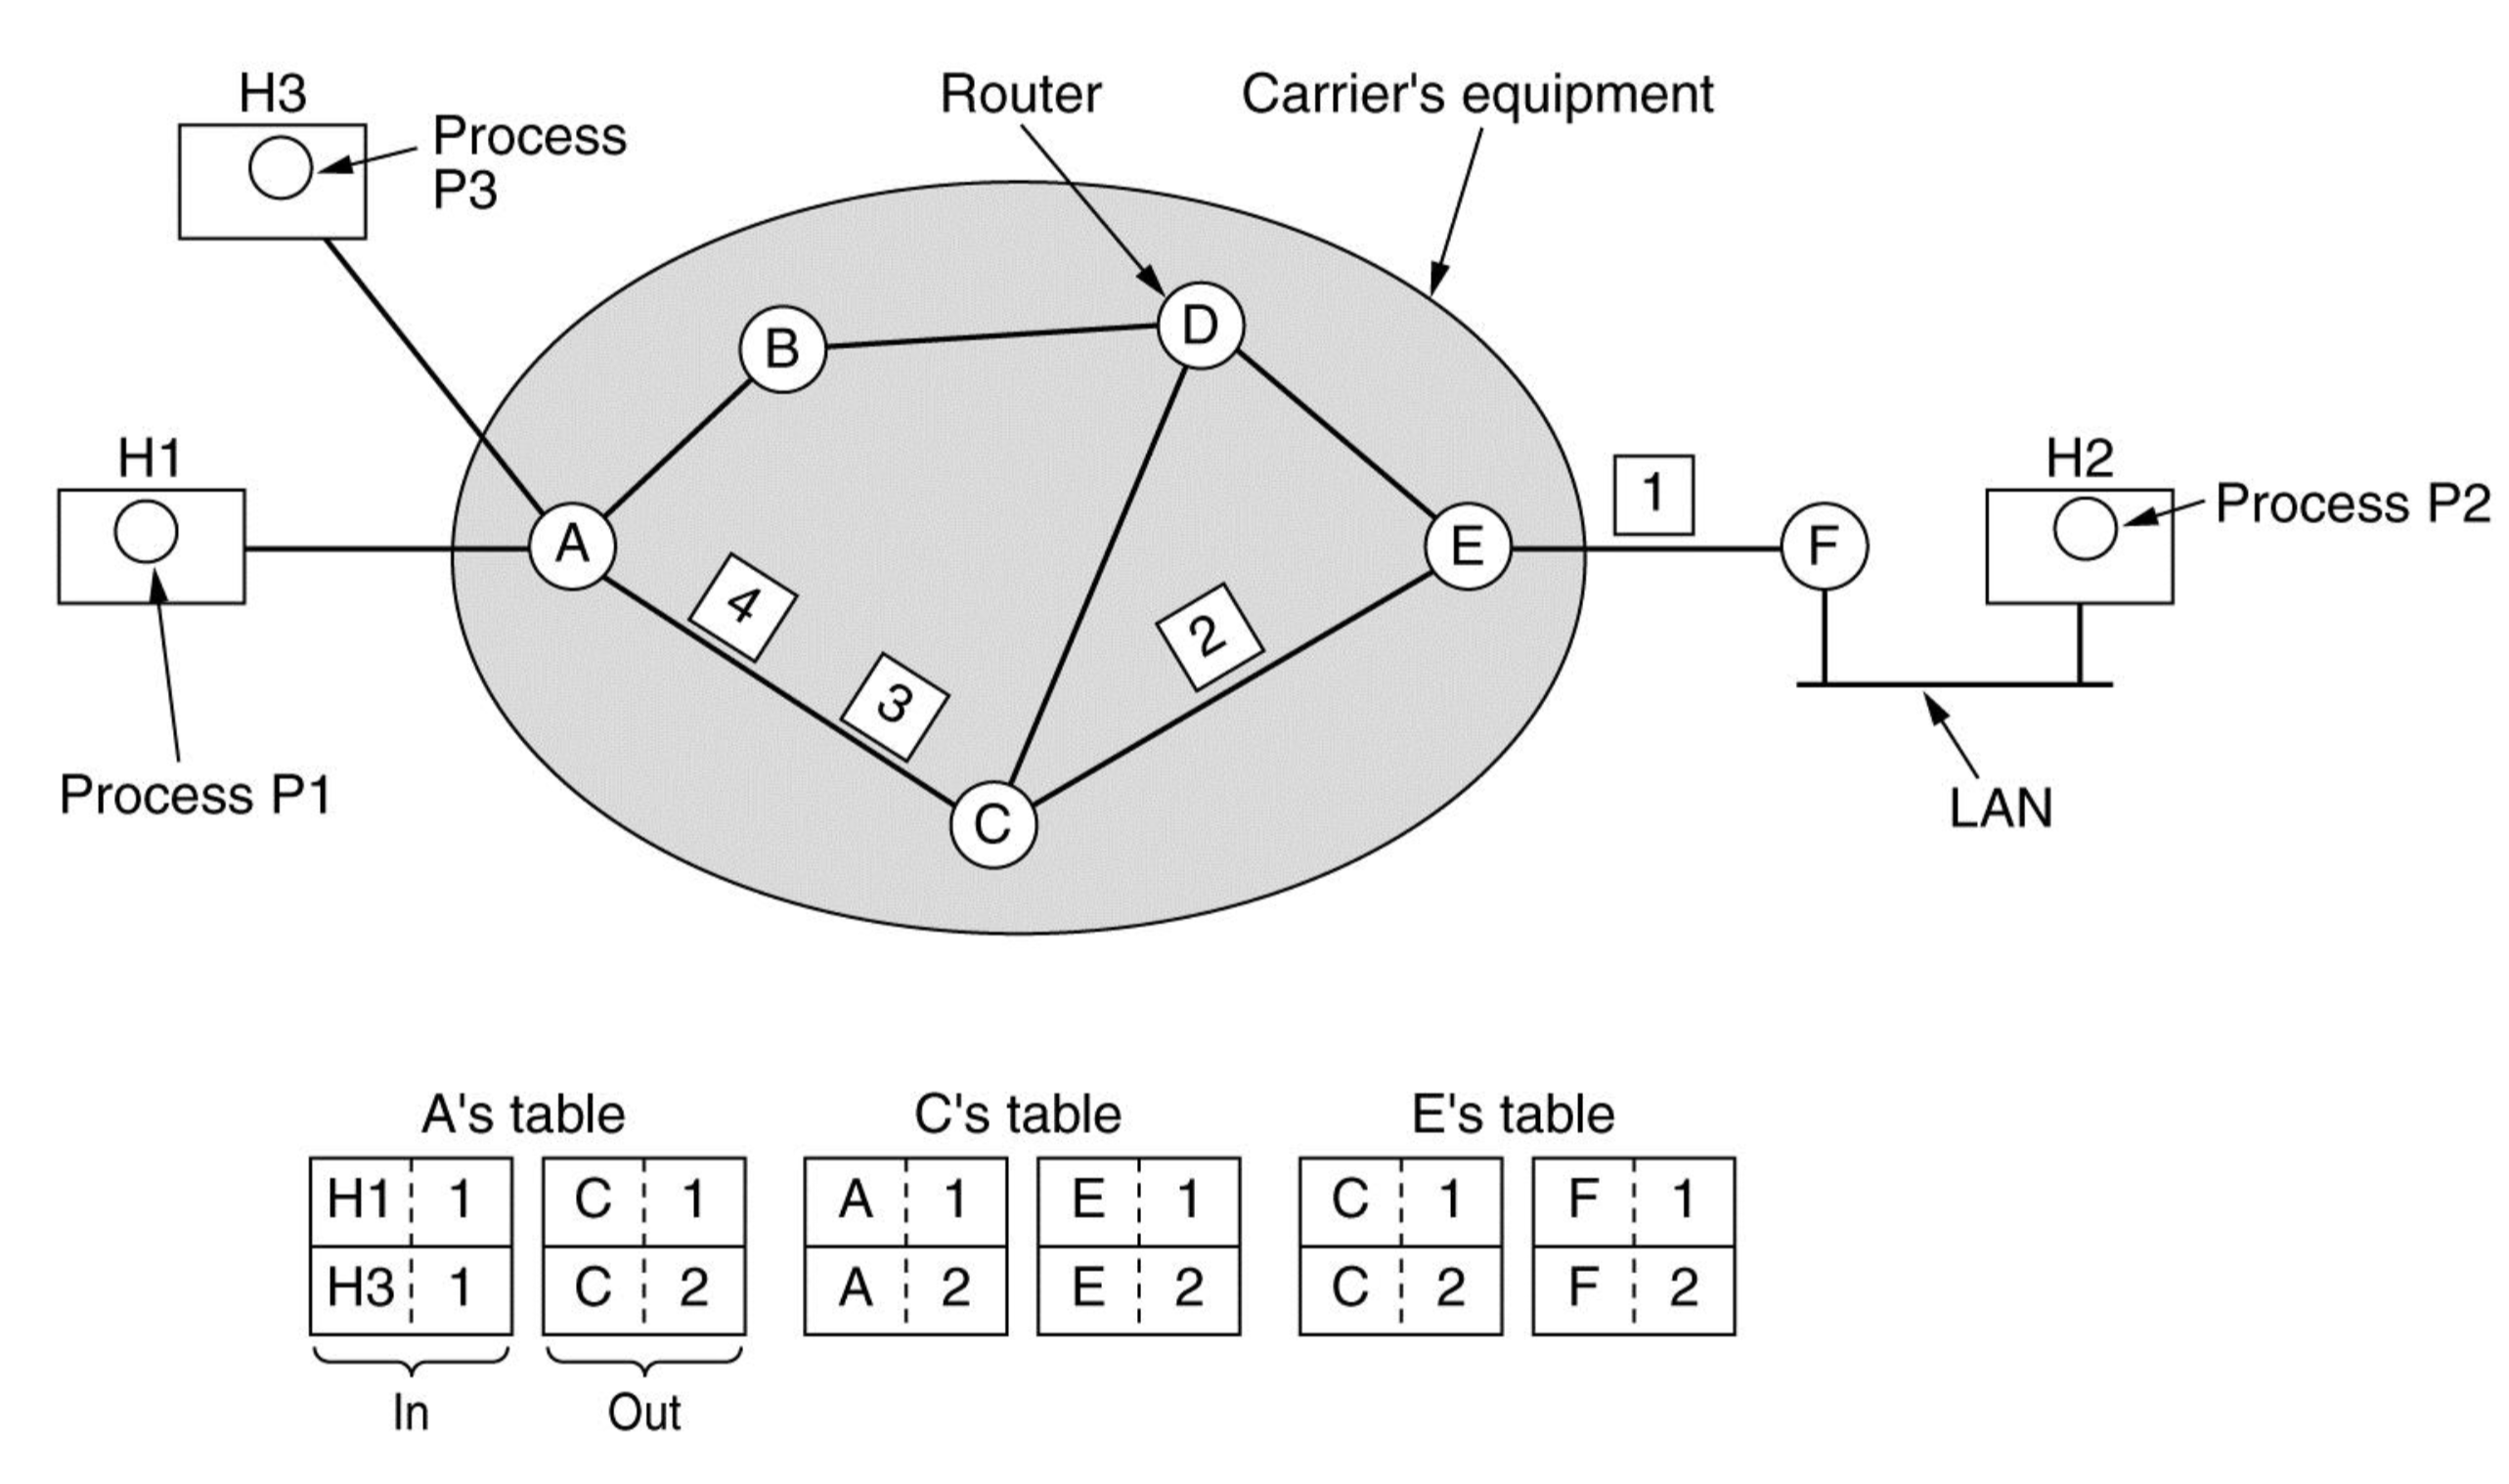
\includegraphics[width=8cm, height=6cm]{./imagenes/orientado.png} 
\end{center}

\par En algunos contextos, a este proceso se le conoce como conmutación mediante 
etiquetas. MPLS (MultiProtocol Label Swithching) es un ejemplo de servicio de red 
orientado a conexión. Se utiliza dentro de las redes de ISP en Internet, en donde los 
paquetes IP se envuelven en un encabezado MPLS que tiene un identificador de 
conexión o etiqueta de 20 bits.
	
\subsection{Comparación entre las redes de circuitos virtuales y las redes de datagramas}
	Dentro de la red existen ventajas y desventajas entre los circuitos virtuales y los 
	datagramas. Una de ellas tiene que ver con el tiempo de configuración y el tiempo de 
	análisis de la dirección. El uso de circuitos virtuales requiere una fase de 
	configuración que necesita tiempo y recursos. Sin embargo, una vez que se paga 
	este precio, es fácil averiguar qué hacer con un paquete de datos en una red de 
	circuitos virtuales: el enrutador sólo usa el número de circuito para buscar en una 
	tabla y encontrar hacia donde va el paquete. En una red de datagramas no se 
	requiere configuración, pero se requiere un procedimiento más complicado para 
	localizar la entrada correspondiente al destino.

	\begin{center} 
		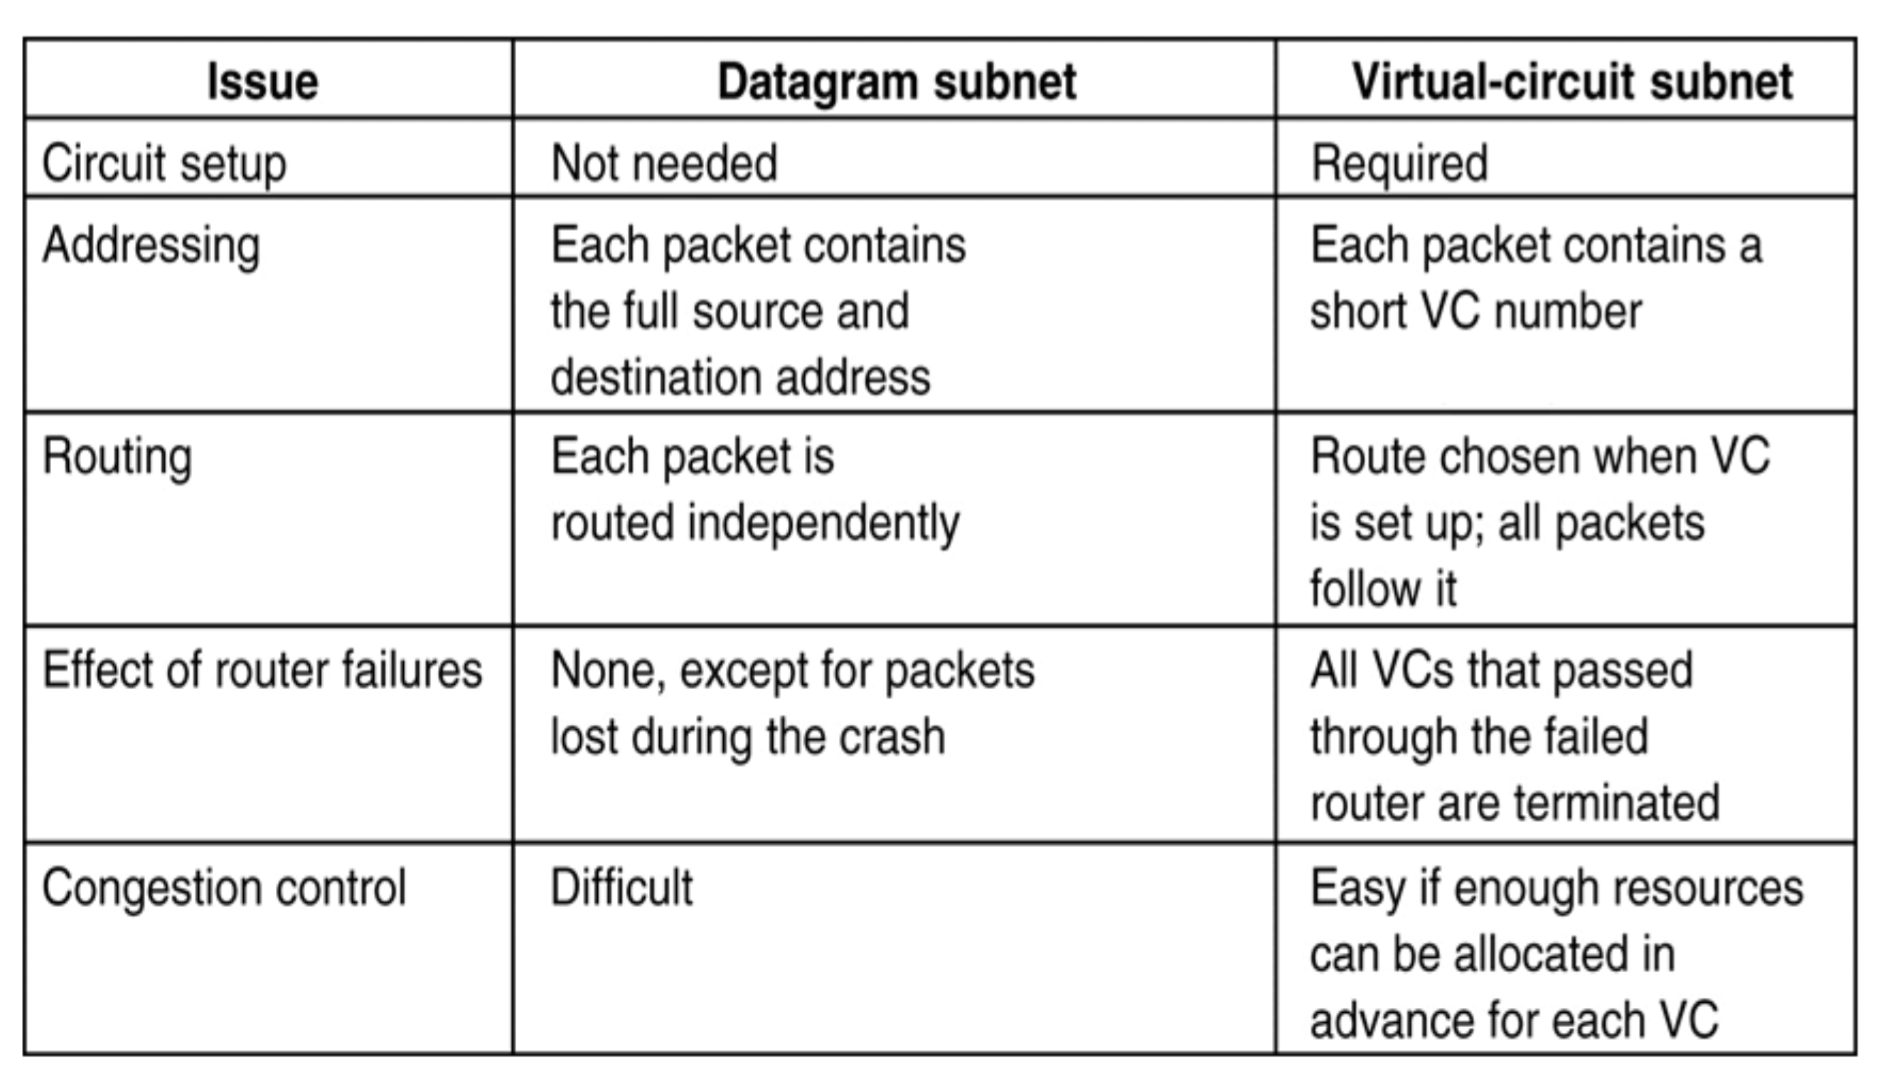
\includegraphics[width=10cm, height=6cm]{./imagenes/comparacion.png}
	\end{center}
	
	\begin{itemize}
		\item Si se cae un enrutador en CV: se pierde su memoria, y todos los CV que 
		pasan por el tendrán que abortarse.
		\item Si se cae un enrutador de datagramas: solo sufrirán los usuarios cuyos 
		paquetes estaban encolados en el enrutador en el momento de la falla, 
		dependiendo de si había confirmado o no su recepción, tal vez ni siquiera todos 
		ellos.
	\end{itemize}


\section{Algoritmos de enrutamiento}
	\par El algoritmo de enrutamiento es aquella parte del software de la capa de red 
	responsable de decidir por cuál línea de salida transmitirá un paquete entrante. Si la 
	red usa datagramas de manera interna, esta decisión debe tomarse cada vez que 
	llega un paquete de datos, dado que la mejor ruta podría haber cambiado desde la 
	última vez. Si la red usa circuitos virtuales internamente, las decisiones de 
	enrutamiento se toman sólo al establecer un circuito virtual nuevo. En lo sucesivo, 
	los paquetes de datos simplemente siguen la ruta ya establecida. Este último caso a 
	veces se llama enrutamiento de sesión, dado que una ruta permanece vigente 
	durante toda una sesión.
	\par En ocasiones es útil distinguir entre el enrutamiento, que es el proceso que 
	consiste en tomar la decisión de cuáles rutas utilizar, y el reenvío, que consiste en la 
	acción que se toma cuando llega un paquete. Podemos considerar que un enrutador 
	tiene dos procesos internos. Uno de ellos maneja cada paquete conforme llega, y 
	después busca en las tablas de enrutamiento la línea de salida por la cual se enviará. 
	Este proceso se conoce como reenvío. El otro proceso es responsable de llenar y 
	actualizar las tablas de enrutamiento. Es ahí donde entra en acción el algoritmo de 
	enrutamiento.
	
	\par Propiedades que todo algoritmo de enrutamiento debe poseer:
		\begin{itemize}
			\item \textbf{Robustez:} una vez que una red entra en operación, deberá
			funcionar 			
			continuamente durante años. Durante ese período habrá fallas de hardware y de 
			software de todo tipo. Los hosts, enrutadores y líneas fallarán en forma 
			repetida y la topología cambiará muchas veces.
			\par El algoritmo de enrutamiento debe ser capaz de manejar los cambios de 
			topología y tráfico sin requerir que aborten todas las actividades en todos los 
			hosts y el reinicio de la red con cada caída de un enrutador.
			\item \textbf{Optimización:} por un lado se intenta minimizar el 
			retardo medio de los paquetes, por otro aumentar al máximo la velocidad real 
			de transporte en la red. 
			\par Estas dos metas están en conflicto. Como término medio muchas redes 
			intentan minimizar el número de saltos que tiene que dar un paquete.
			La reducción de la cantidad de saltos reduce el retardo y también el consumo 
			de ancho de banda, lo que a su vez mejora la velocidad real de transporte.
			\item \textbf{Equidad:} implica que todos los hosts deben poder usar la subred 
			ya sea para enviar o para recibir.
			\par La equidad y la optimización son con frecuencia metas contradictorias. Por 
			ende se requiere de un punto medio entre la eficiencia global y la equidad hacia 
			las conexiones individuales.
			\item \textbf{Sencillez:} apenas requiere comentarios. Es algo que todos los 
			algoritmos de enrutamiento deberían tener. 
			\item \textbf{Estabilidad:} también es una meta importante para el algoritmo 
			de enrutamiento. Existen algoritmos de enrutamiento que nunca convergen 
			hacia un conjunto de rutas fijo, sin importar el tiempo que permanezcan en 
			operación. Un algoritmo estable alcanza el equilibrio y lo conserva. Además 
			debe converger con rapidez, ya que se puede interrumpir la comunicación hasta 
			que el algoritmo de enrutamiento haya llegado a un equilibrio.
		\end{itemize}
		
		\par Los algoritmos de enrutamiento pueden agruparse en dos clases: 
		\begin{enumerate}
		
			\item  \textbf{\emph{Los algoritmos no adaptativos: }} no basan sus 
			decisiones de enrutamiento en mediciones o estimaciones del tráfico y la 
			topología actuales.
			\begin{itemize}
				\item La decisión de qué ruta se usará para ir de I a J se toma por 
				adelantado.
				\item A esto se lo conoce como enrutamiento estático.
				\item Ejemplos: enrutamiento de caminos más cortos, inundación.
			\end{itemize}
			
			\item \textbf{\emph{Los algortimos adaptativos:}} cambian sus decisiones de 
			enrutamiento para reflejar los cambios de topología, y por lo general también 
			del tráfico.
			\par Los algoritmos adaptivos difieren en:
			\begin{itemize}
				\item El lugar donde obtienen su información, localmente en los enrutadores 
				adyacentes o en todos los enrutadores.
				\item El momento de cambio de sus rutas (i.e. de sus tablas de 
				enrutamiento). Hay varias opciones, ellas son: cada cierta cantidad de 
				segundos, cuando cambia la carga, o cuando cambia la topología.
				\item La métrica usada para la optimización: distancia, número de saltos, 
				tiempo estimado de tránsito, etc.
			\end{itemize}
			\par Ejemplos: enrutamiento de vector de distancia, enrutamiento de estado de 
			enlace.		
		\end{enumerate}

\subsection{Principio de optimización}
	\par Establece que si un enrutador \textit{J} está en ruta óptima 
	del enrutador \textit{I} al enrutador \textit{K}, entonces la ruta óptima de \textit{J}
	a \textit{K} también está en la misma ruta.
	\par Como consecuencia directa del principio de optimización, podemos ver que el 
	grupo de rutas óptimas de todos los orígenes a un destino dado forman un árbol con 
	raíz en el destino. Dicho árbol se conoce como \textit{árbol sumidero} y se ilustra en 
	la figura, donde la métrica de distancia es el número de saltos. El objetivo de todos 
	los algoritmos de enrutamiento es descubrir y usar los árboles sumidero para todos 
	los enrutadores.
	
	\begin{center}
		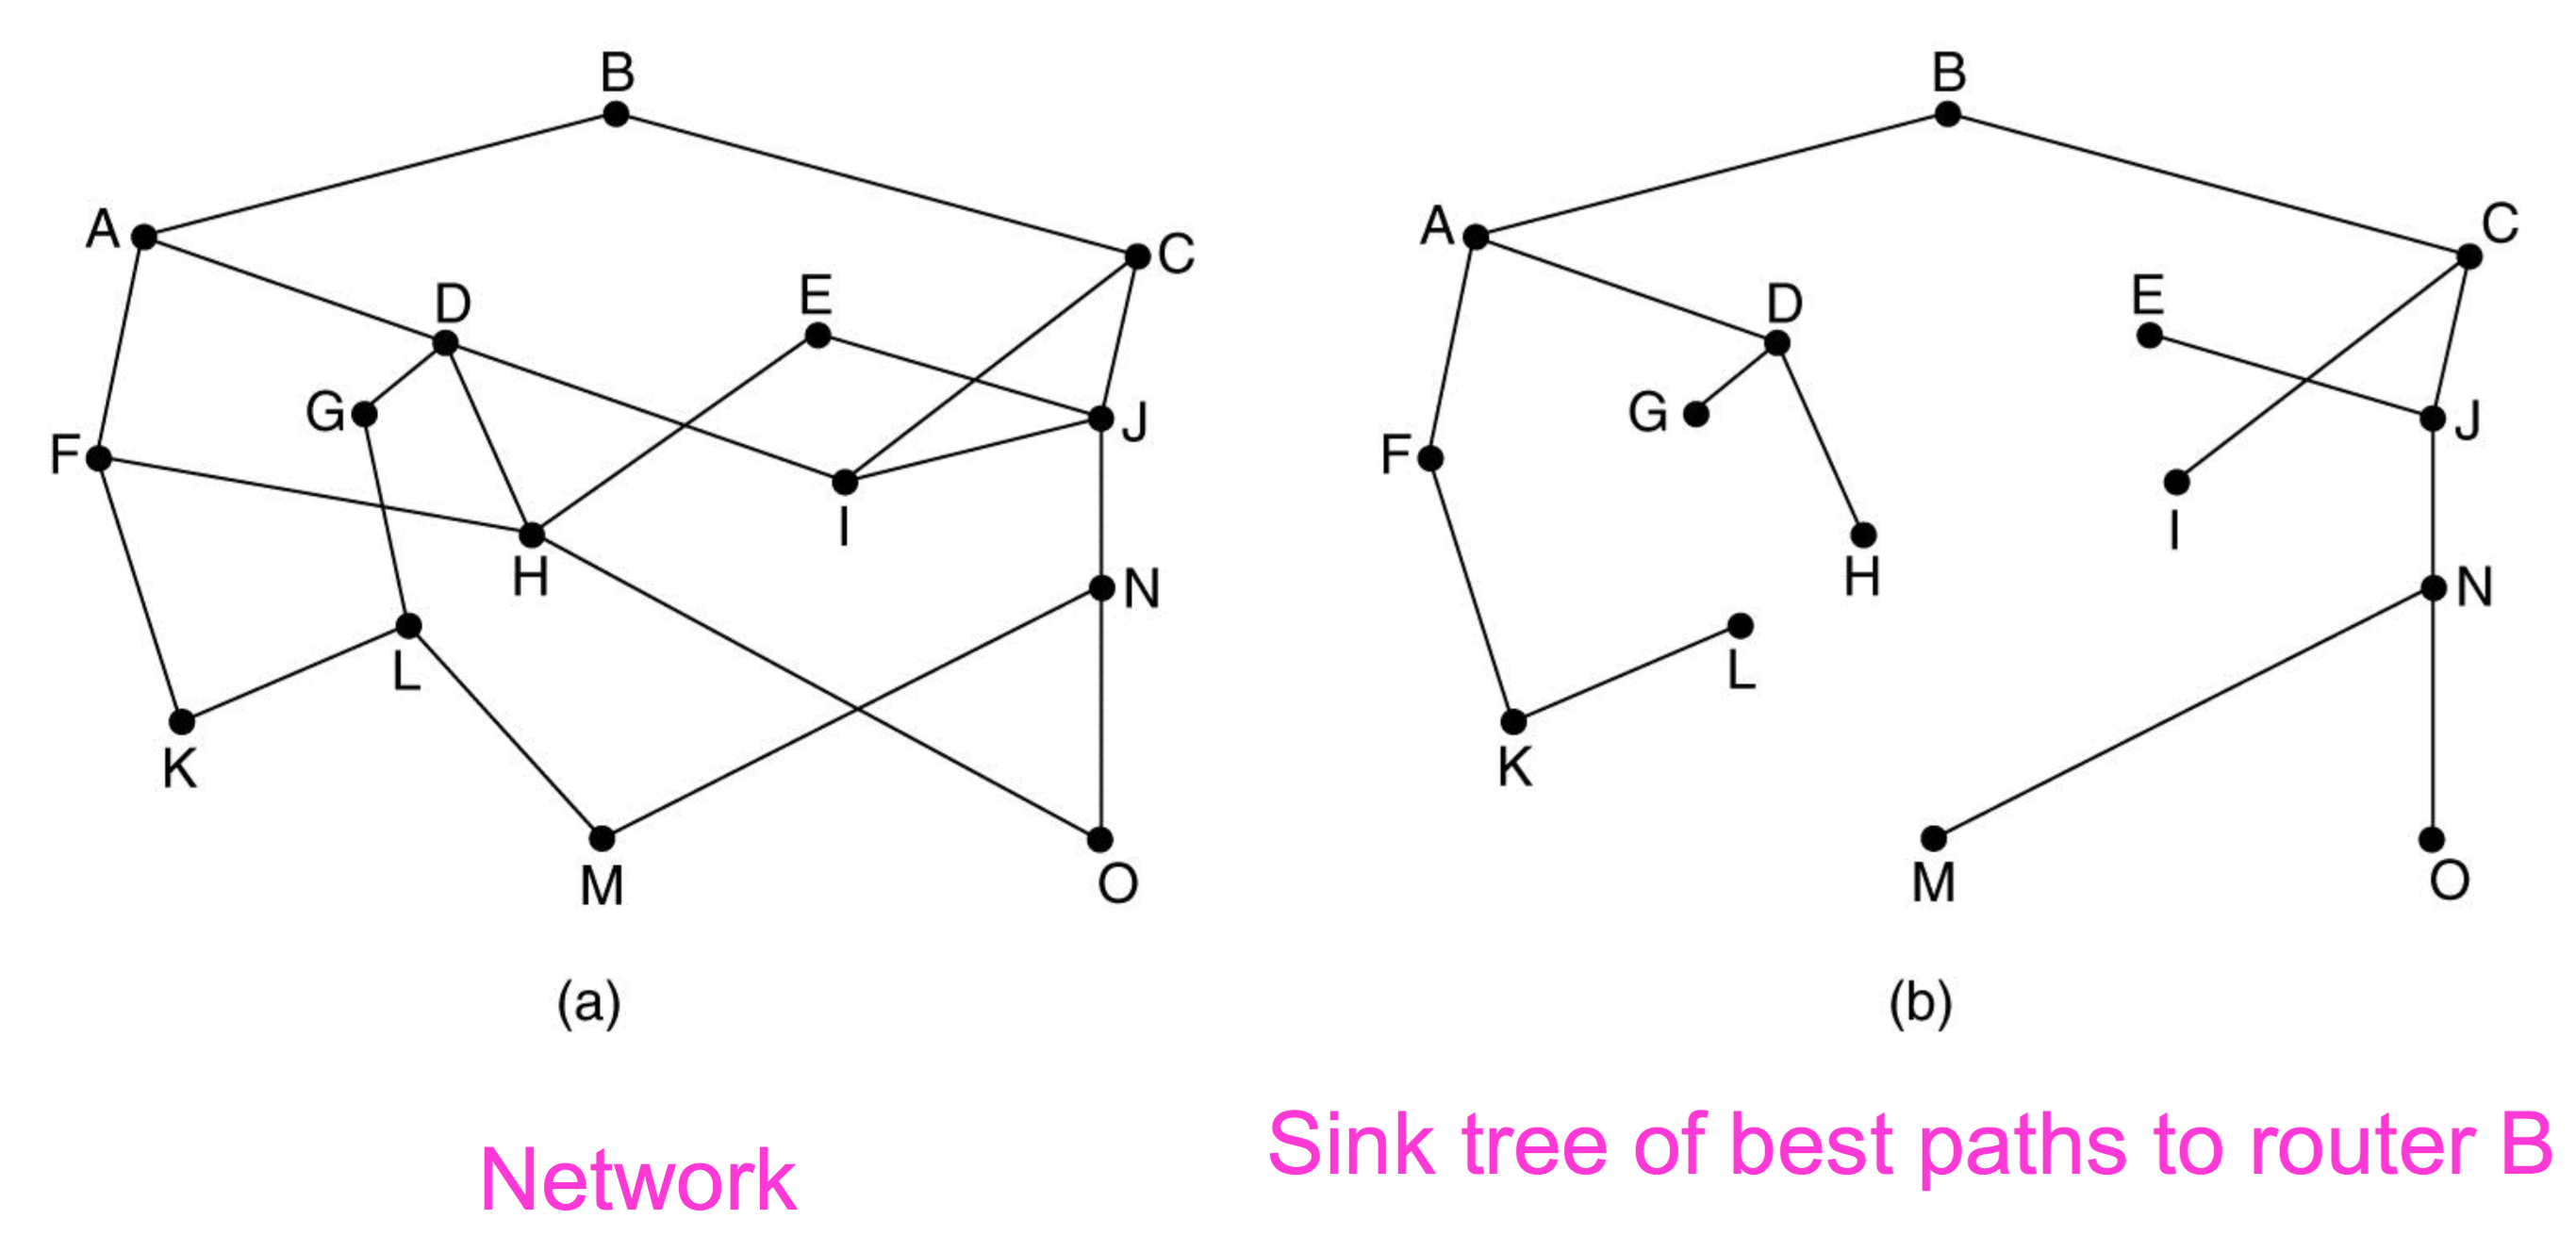
\includegraphics[width=10cm, height=6cm]{./imagenes/optimalidad.png}
	\end{center}

	\par Por ende la meta de todos los algoritmos de enrutamiento es descubrir y utilizar 
	los árboles sumideros de todos los enrutadores.
	
	\par Comenzaremos estudiando algoritmos estáticos, los mismos no son muy 
	buenos, pero veremos que pequeñas variantes de ellos son usados por los algoritmos 
	adaptivos.

\subsection{Algoritmo de la ruta más corta}
	\par La idea es construir un grafo de la red, en donde cada nodo del grafo 
	representa un enrutador y cada arco del grafo representa una línea o enlace de 
	comunicaciones. Para elegir una ruta entre un par específico de enrutadores, el 
	algoritmo simplemente encuentra la ruta más corta entre ellos en el grafo.

	\par Una manera de medir la longitud de una ruta es mediante el número de saltos. 
	Otra métrica es la distancia geográfica en kilómetros, etc. En el caso más general, las 
	etiquetas de los arcos podrían calcularse como función de la distancia, ancho de 
	banda, tráfico medio, costo de comunicación, longitud media de las colas, retardo 
	medio, y otros factores.

	\par Se conocen varios algoritmos para calcular la ruta más corta entre dos nodos de 
	un grafo. Uno de éstos se debe a Dijkstra.


	\par \textbf{Algoritmo de Dijktra:}
		\begin{itemize}
			\item Calculamos la ruta más corta posible entre \emph{s} y \emph{t}
			comenzando por el nodo de destino \emph{t}.
			\item El algoritmo calcula un árbol sumidero en la subred.
			\item Cada nodo se etiqueta con su distancia al nodo de origen a través de la 	
			mejor ruta conocida (al comienzo todos los nodos tienen etiqueta <). Mientras 
			avanza el algoritmo las etiquetas pueden cambiar reflejando mejores rutas.
 			\item Una etiqueta puede ser tentativa o permanente. Inicialmente todas las 
 			etiquetas son tentativas. Cuando se descubre que una etiqueta representa la 
 			ruta más corta del origen a ese nodo, se vuelve permanente y no cambia más.
			\item Se tiene una iteración para la cua lsiempre hay un nodo de trabajo. Ese 
			nodo de trabajo es el nodo tentativo con la menor etiqueta calculado en el paso 
			de iteración anterior (Inicialmente el nodo de trabajo es \emph{t}).
			
			En cada paso de la iteración se actualizan las etiquetas de los nodos tentativos 
			siempre y cuando el nodo de trabajo ayude a encontrar una ruta mejor.
		\end{itemize}

	\begin{center}
	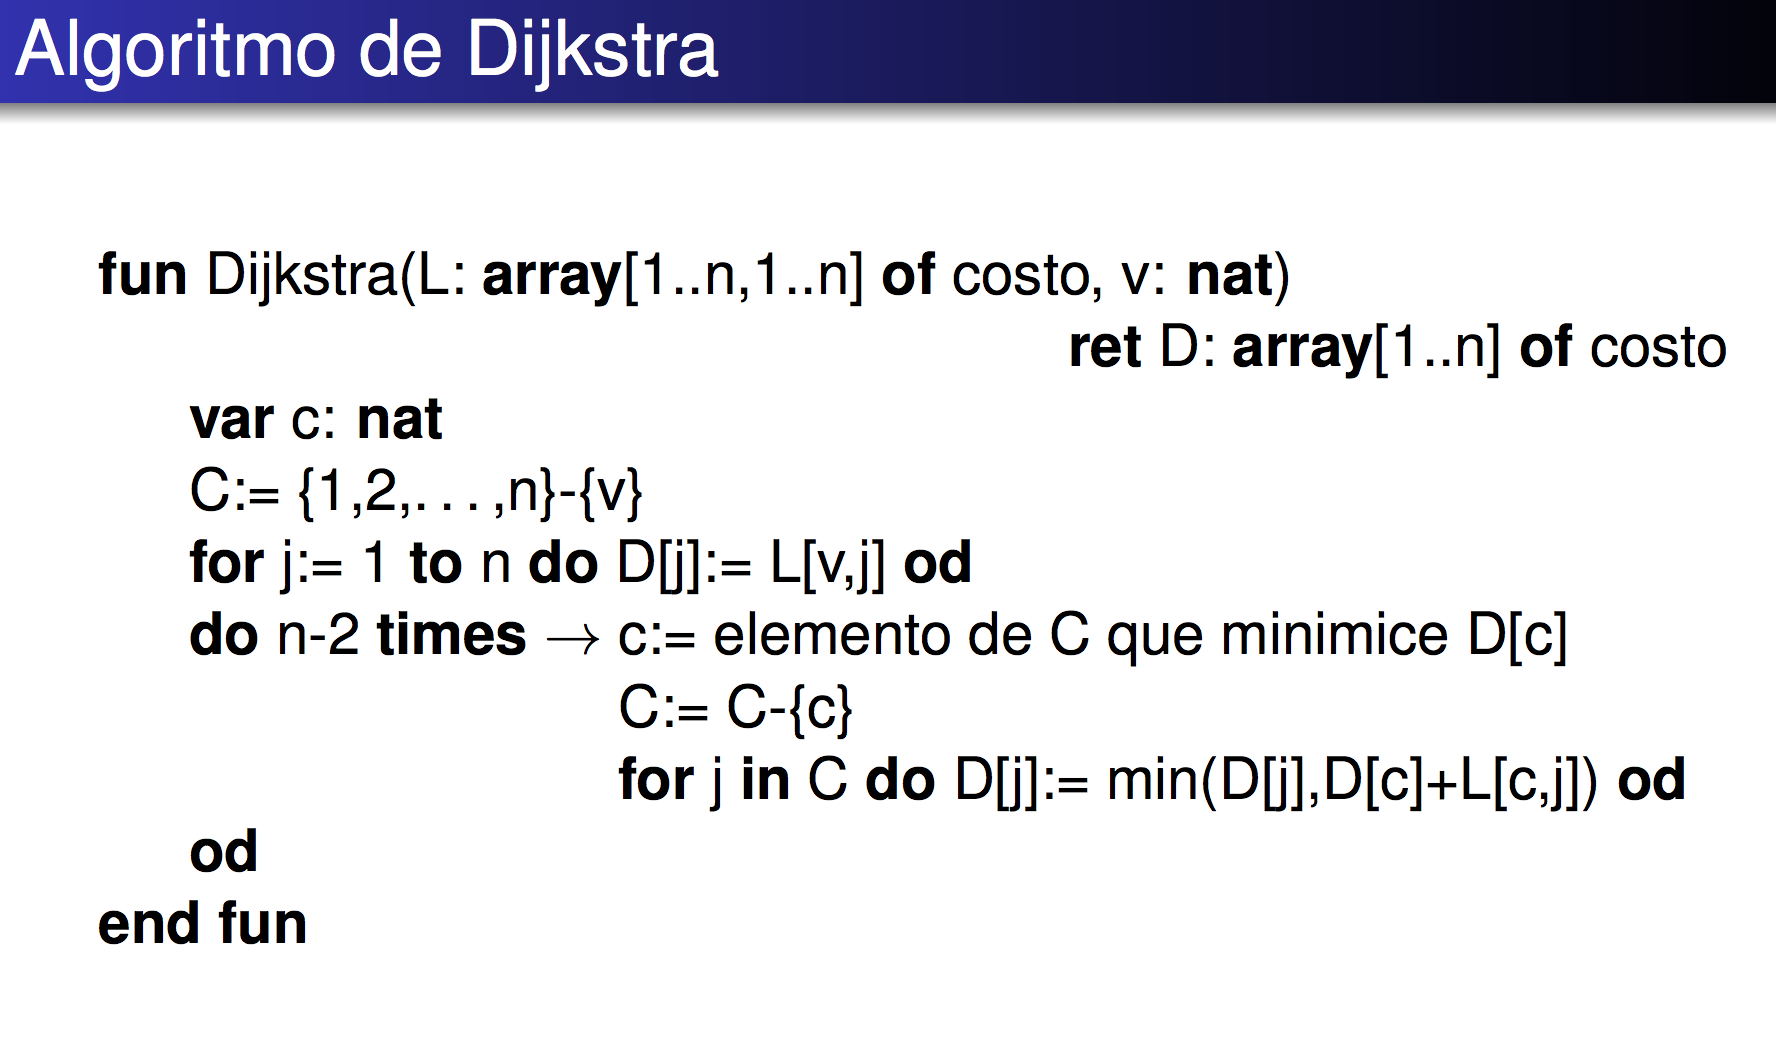
\includegraphics[width=8cm, height=5cm]{./imagenes/dijktra.png} 

	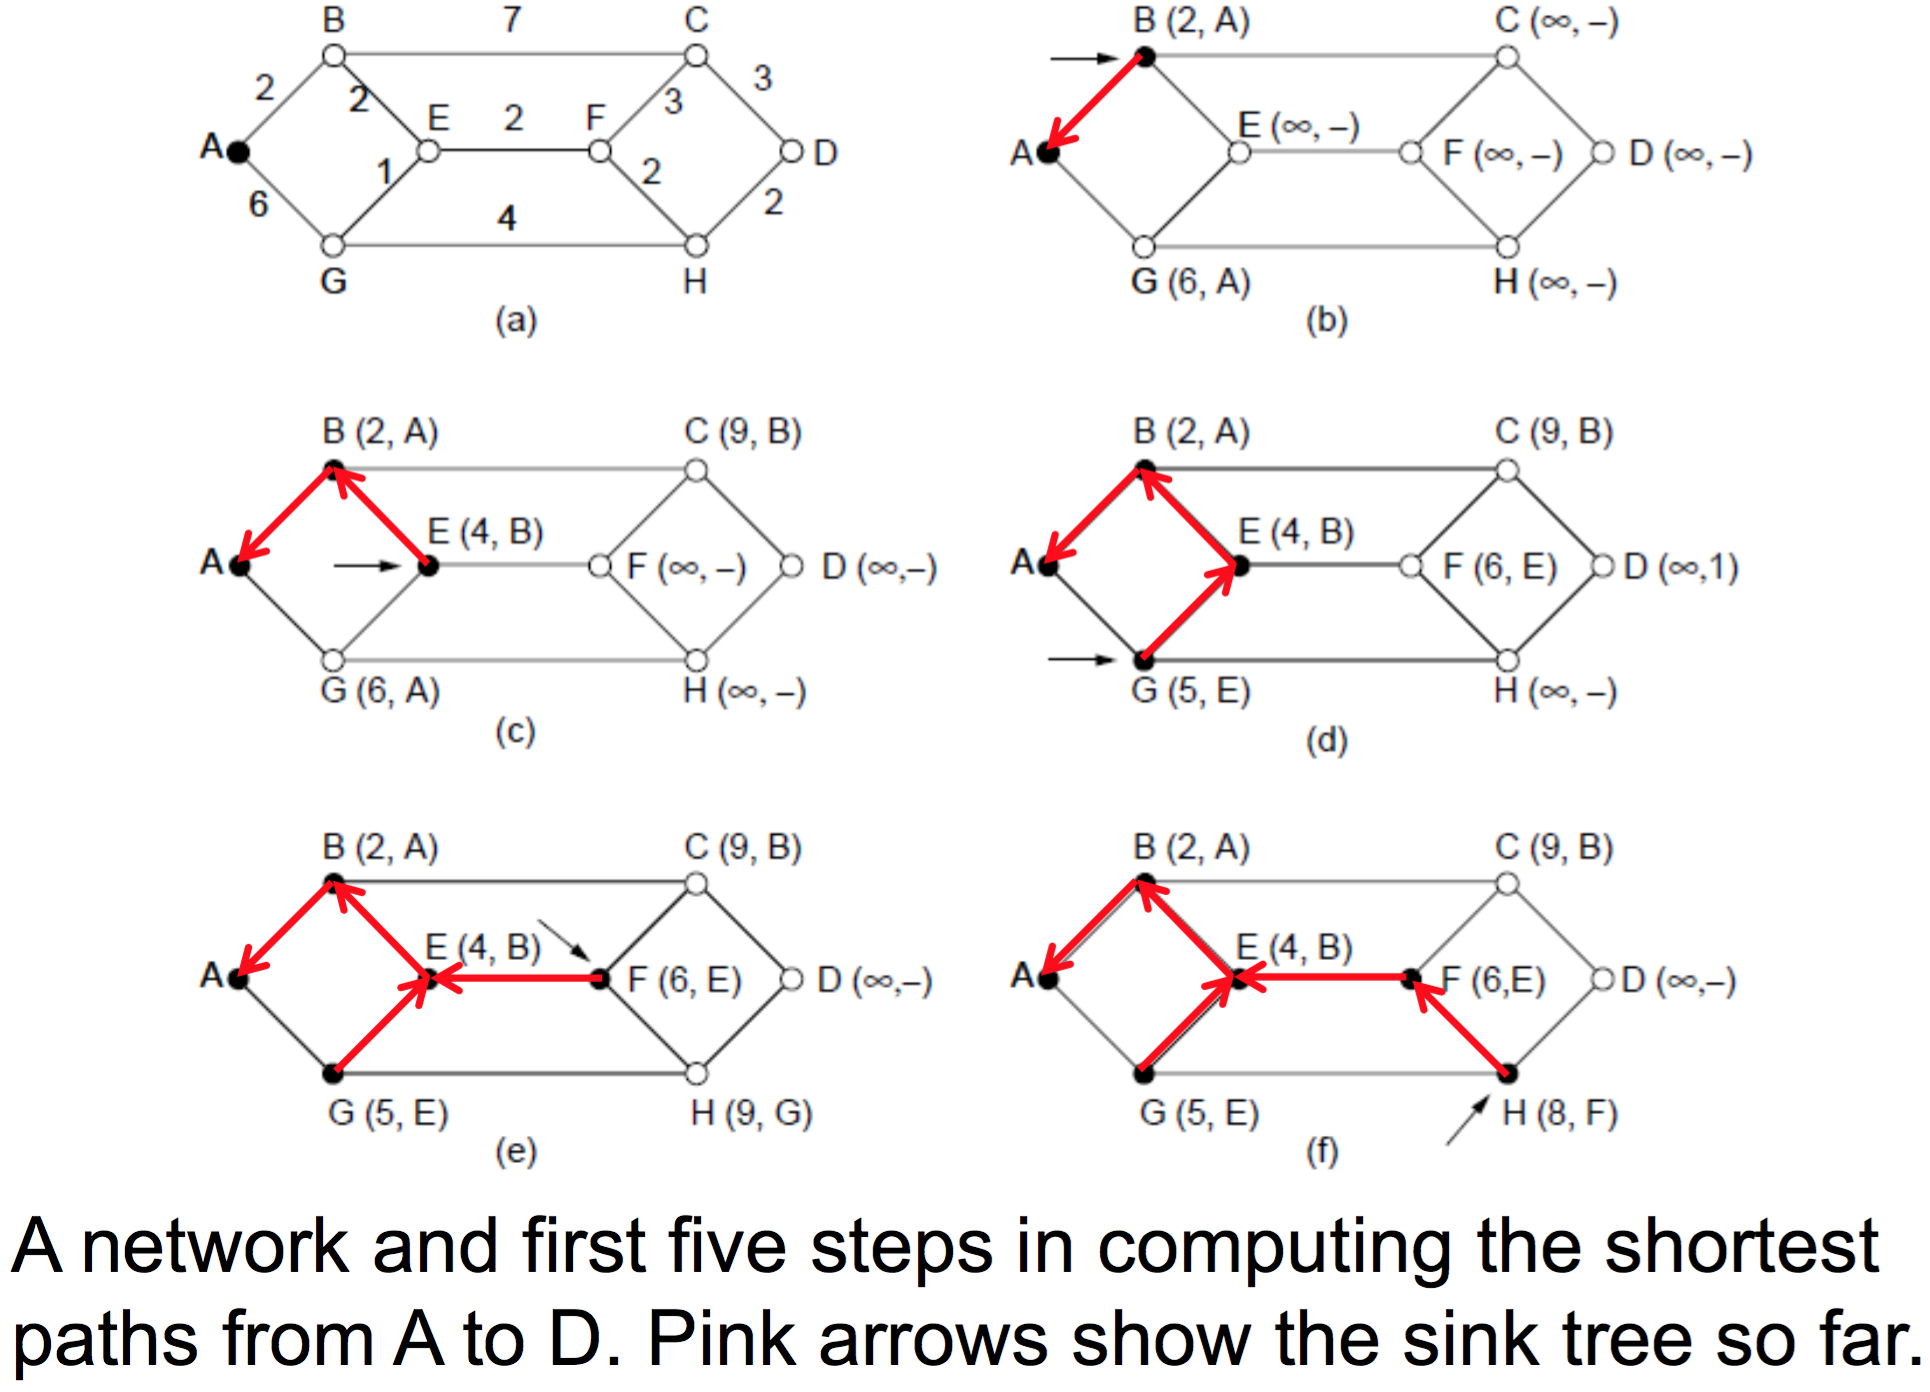
\includegraphics[width=10cm, height=6cm]{./imagenes/caminos.png}
	\end{center}

\subsection{Inundación}
	\par Otro algoritmo estático es la inundación, en la que cada paquete de entrada se 
	envía por cada una de las líneas de salida, excepto aquella por la que llegó.
    Esta idea tiene un problema, la inundación genera grandes cantidades de paquetes 
    duplicados; a menos que se tomen algunas medidas para limitar el proceso. Veamos 
    algos de estas ideas:

	\begin{itemize}
		\item Solución 1: integrar un contador de saltos en el encabezado de cada 
		paquete, que disminuya con cada salto y el paquete se descarte cuando el 
		contador llega a 0. Lo ideal es inicializar el contador de saltos a la longitud de la 
		ruta entre el origen y el destino. Si el emisor desconoce el tamaño de la ruta, 
		puede inicializar el contador al peor caso, es decir, al diámetro total de la subred.
		
		\item Solución 2: llevar un registro de los paquetes difundidos para evitar 
		enviarlos por segunda vez. Hacer que el enrutador de origen ponga un número de 
		secuencia en cada paquete que recibe de sus hosts. Para cada enrutador de origen 
		hay una lista con los números de secuencia originados en ese enrutador que ya ha 
		visto. Si un paquete de entrada está en la lista, no se difunde.

		Para evitar que las listas crezcan sin límites podemos agregar una columna 
		contador que indica el mayor número de secuencia tal que llegaron paquetes con 
		todos los numeros de secuencia anteriores desde ese enrutador de origen.
		
		\item Solución 3: Una variación de la inundación, un poco mas práctica, es la 
		inundación selectiva. Los enrutadores no envían cada paquete de entrada por 
		todas las líneas, sino solo por aquellas que van aproximadamente en la dirección 
		correcta.

		A nivel de información, se necesita saber en qué  dirección va cada línea y en qué 
		dirección está el destino.
		
		\par La inundación no es práctica en la mayoría de las aplicaciones, pero tiene
		algunos usos, por ejemplo, en aplicaciones militares, en aplicaciones distribuidas 
		de bases de datos. La inundación siempre elige la ruta más corta posible porque 
		escoge en paralelo todas las rutas posibles. En consecuencia ningún otro 
		algoritmo puede producir un retardo más corto (si ignoramos la sobrecarga 
		generada por el proceso de inundación mismo).
		
	\end{itemize}
		
\subsection{Enrutamiento por vector de distancia}

	\par 	Existen dos algoritmos dinámicos que son los más populares: el enrutamiento 
	por vector de distancia y el enrutamiento por estado del enlace. En esta sección 
	veremos el primer algoritmo, en la siguiente estudiaremos el segundo.
	\par En el enrutamiento por vector de distancia, cada enrutador mantiene una tabla 
	de enrutamiento indizada por cada enrutador de la red. Esta entrada consta de dos 
	partes:
	\begin{itemize}
			\item La línea preferida de salida a usar para ese destino
			\item Una estimación del tiempo o distancia a ese destino. 
	\end{itemize}
	\par La distancia se podría medir como la cantidad de saltos, o se podría usar otra 
	métrica, como vimos al calcular las rutas más cortas. 
	\par 	Estas tablas se actualizan intercambiando información con los vecinos. Este 
	algoritmo se usó en Internet con el nombre \textbf{RIP}.
	
	\par Se supone que el enrutador conoce la “distancia” a cada uno de sus vecinos.
		\begin{itemize}
			\item Si la métrica es de saltos, la distancia es un salto.
			\item Si la métrica es la longitud de la cola, el enrutador simplemente examina 
			cada cola.
			\item Si la métrica es el retardo, el enrutador puede medirlo con paquetes de 
			ECO que el receptor simplemente marca con la hora y los regresa tan rápido 
			como puede.
		\end{itemize}
	\par Suponga que el retardo se usa como métrica y que el enrutador conoce el 
	retardo a cada uno de sus vecinos. Una vez cada \textit{T} mseg, cada enrutador 
	envía a todos sus vecinos una lista de sus retardos estimados a cada destino.
	También recibe una lista similar de cada vecino. Imagine que la tabla
	\textit{$T_{x}$} acaba de llegar del vecino \textit{X}, en donde \textit{$X_{i}$} es 
	la 	estimación respecto al tiempo que le toma llegar al enrutador \textit{i}. Si el 	
	enrutador sabe que 	el retardo a 	\textit{X} es de \textit{$m_{x}$} mseg, también 
	sabe que puede llegar al enrutador \textit{i} a través de \textit{X} en 
	\textit{$X_{i}$} $+$ \textit{$m_{i}$} mseg. Al efectuar este cálculo para cada 
	vecino, un enrutador puede encontrar la estimación que parezca ser la mejor y usar 
	esa estimación, así como el enlace correspondiente, en su \textbf{nueva tabla de 
	enrutamiento}. Cabe mencionar que en este cálculo no se utiliza la antigua tabla de 
	enrutamiento.

	\par El enrutamiento por vector reacciona con rapidez a las buenas noticias, pero 
	con lentitud ante las malas. Considere un enrutador cuya mejor ruta al destino 
	\textit{X} es larga. Si en el siguiente intercambio el vecino \textit{A} informa 
	repentinamente un retardo corto a \textit{X}, el enrutador simplemente se conmuta 
	a modo de usar la línea a A para enviar tráfico hasta X.
Supongamos que la métrica de retardo es el numero de saltos.
 Las buenas noticias se difunden a razón de un salto por intercambio.
 En una subred cuya ruta mayor tiene una longitud de N saltos, en un lapso de N intercambios todo el mundo sabrá sobre las líneas y enrutadores recientemente revividos.
La razón de porque las malas noticias viajan con lentitud es: ningún enrutador jamás tiene un valor mayor en más de una unidad que el mínimo de todos sus vecinos.
Gradualmente todos los enrutadores elevan cuentas hacia el infinito, pero el número de intercambios requeridos depende del valor numérico usado para el infinito.
Si la métrica usada es el número de saltos, es prudente hacer que el infinito sea igual a la ruta más larga más 1.

Si la métrica es el retardo de tiempo no hay un límite superior
bien definido,
se necesita un valor alto para evitar que una ruta con un retardo grande sea tratada como si estuviera desactivada.
Este es el problema de la cuenta hasta el infinito.
Se han hecho varios intentos para resolverlo, pero ninguno funciona bien
en general.
La esencia del problema consiste en que cuando X indica Xi a E, E no tiene forma de saber si el destino i está en alguna ruta en funcionamiento.

\subsection{Enrutamiento por estado del enlace}
	\par La idea detrás del enrutamiento por estado del enlace es bastante simple y 
	se puede enunciar en cinco partes. Cada enrutador debe realizar lo siguiente para 
	hacerlo funcionar:

	\begin{enumerate}
		\item Descubrir a sus vecinos y conocer sus direcciones de red: esto lo realiza 
		enviando un paquete HELLO especial a cada línea punto a punto. Se espera que 
		el 	enrutador del otro extremo regrese una respuesta indicando quién es. Estos
		nombres deben ser globalmente únicos.

		\item Establecer la métrica de distancia o de costo para cada uno de sus vecinos:
		el AEEE requiere que cada enrutador tenga una idea razonable del retardo a cada 
		uno de sus vecinos. Una forma de determinarlo es enviar un paquete ECHO 
		especial a través de la línea, una vez que llegue al otro extremo, éste debe 
		regresarlo inmediatamente.

		\par Si se mide el tiempo de ida y vuelta y se divide por $2$, el enrutador emisor 
		puede tener una idea razonable del retardo. Pero esto tiene un problema, ya que 
		el algoritmo asume de manera implícita que los retardos son simétricos, lo cual no 
		siempre es el caso.

		\par Un aspecto importante es si se debe tener en cuenta la carga al medir el 
		retardo. Para considerar la carga, el temporizador debe iniciarse cuando el paquete 
		ECHO se ponga en la cola. Para ignorar la carga, el temporizador debe iniciarse 
		cuando el paquete ECHO alcance el frente de la cola.
		
		\par Cuando un enrutador puede escoger entre dos líneas con el mismo ancho de 
		banda, una con carga alta continua y otra sin ella, considerará como ruta más 
		corta la de la línea sin carga. Esta selección resultará en un mejor desempeño. 		
		Desgraciadamente también hay un argumento en contra de la inclusión de la carga 
		en el cálculo del retardo.

		\item Construir un paquete que indique todo lo que acaba de aprender: Cada 
		enrutador construye un paquete des estado de enlace (LSP) que contiene todos 
		los datos:
		\begin{itemize}
			\item Identidad del emisor
			\item Numero de secuencia
			\item Edad
			\item Lista de (vecino, retardo al vecino)
		\end{itemize}

		\par los paquetes deben ser construirlos de manera periódica, es decir, a 
		intervalos regulares o cuando ocurra un evento significativo, como la caída o la 
		reactivación de la línea o de un vecino, o el cambio apreciable de sus propiedades.

		\item Enviar este paquete a todos los demás enrutadores y recibir paquetes de 		
		ellos: la parte más complicada del algoritmo es la distribución confiable de los 
		paquetes de estado del enlace.
		
		\par La idea fundamental es usar inundación para distribuir los paquetes de 
		estado 
		del enlace, llevando un registro de los paquetes difundidos. A fin de mantener 
		controlada la inundación, cada paquete contiene un número de secuencia que se 
		incrementa con cada paquete nuevo enviado (desde su enrutador de origen).
		\par Los enrutadores llevan el registro de todos los pares (enrutador de origen, 
		secuencia) que ven. Para cada enrutador de origen el paquete recibido con 
		número de secuencia más grande es el que importa, los anteriores no.

		\item Calcular la ruta más corta a todos los demás enrutadores.
	\end{enumerate}



\subsection{Enrutamiento jerárquico}
\subsection{Enrutamiento por difusión}
\section{Algoritmos de control de congestión}
\subsection{Métodos para el control de la congestión}
\subsection{Enrutamiento consciente del tráfico}
\subsection{Control de admisión}
\subsection{Regulación del tráfico}
\subsection{Desprendimiento de carga}

\section{La capa de internet}
	\subsection{El protocolo IP versión 4}
	\subsection{Direcciónes IP}


\subsection{Protocolos de control de Internet}


%LIsta
\subsubsection{ARP: Protocolo de Resolución de Direcciones}

	\par Aunque en internet una máquina tiene una o más direcciones IP, estas no pueden usarse para enviar paquetes debido a que el hardware de la capa de enlace de datos no entiende las direcciones de internet. Hoy día la mayoría de los hosts de las compañías y las universidades se une a una LAN por una tarjeta de red que solo entiende direcciones LAN. Por ejemplo cada tarjeta Ethernet viene provista de fábrica con una dirección Ethernet de 48 bits, las tarjetas envían y reciben tramas basadas en direcciones Ethernet de 48 bits pero no saben nada de direcciones IP.
	
	\par La pregunta ahora es: ¿Cómo se convierten las direcciones IP en direcciones de la capa de enlace de datos, como Ethernet?. La idea sería que el host de origen dé salida a un paquete de difusión hacia Ethernet preguntando: ¿Quién posee una dirección IP w.x.y.z ?. La difusión llegará a cada máquina en Ethernet y cada una verificará su dirección IP. Al host de destino le bastará con responder con su dirección de Ethernet E y de este modo el host de origen aprende que la dirección IP de w.x.y.z está en el host con la dirección de Ethernet E. Casi cada máquina en Internet ejecuta ARP.

	\par La ventaja de usar ARP es la sencillez. Solo se tiene que asignar a cada máquina una dirección IP y decidir respecto de las máscaras de subred. ARP hace el resto.
	
	\par Se pueden hacer optimizaciones para que ARP funcione con más eficiencia.
	
		\begin{itemize}
			\item \underline{Optimización 1:} una vez que una máquina ha ejecutado ARP, guarda el resultado en caso de que en poco tiempo tenga que ponerse de nuevo en contacto con la misma máquina. La próxima vez encontrará la correspondencia en su propia caché, eliminando así la necesidad de una segunda difusión.

			\item \underline{Optimización 2:} en muchos casos el host de destino necesitará devolver una respuesta, forzando también a que se ejecute el ARP para determinar la dirección Ethernet del emisor. Esta difusión de ARP puede evitarse teniendo el host de origen que incluir su correspondencia IP a Ethernet en el paquete ARP. Cuando la difusión de ARP llega al host de destino, se introduce la dirección IP y de Ethernet del origen en el caché del host 2 para su uso futuro.
			
			\item \underline{Optimización 3:} cada máquina difunde su correspondencia cuando arranca, esto se hace mediante un ARP que busca su propia dirección IP. No debe haber una respuesta, pero un efecto lateral de la difusión es hacer una entrada en el caché ARP de todas las máquinas, si llega inesperadamente una respuesta, es que la misma dirección IP se ha asignado a dos máquinas. La más reciente debe avisar y no arrancar.
		\end{itemize}

	\par Para permitir que las asociaciones cambien, por ejemplo, al configurar un host para que use una nueva dirección IP (pero que mantenga su vieja dirección Ethernet), las entradas en la caché ARP deben expirar después de unos cuantos minutos.
	
	\par Cuando el host de origen y el host de destino están en distintas Ethernet LAN 1 y LAN 2 respectivamente separadas por enrutadores, si se usa ARP fallará ya que el host de destino no verá la difusión (los enrutadores no envían difusiones a nivel Ethernet). Veamos este problema con un ejemplo en la siguiente figura.
	
		\begin{center}
			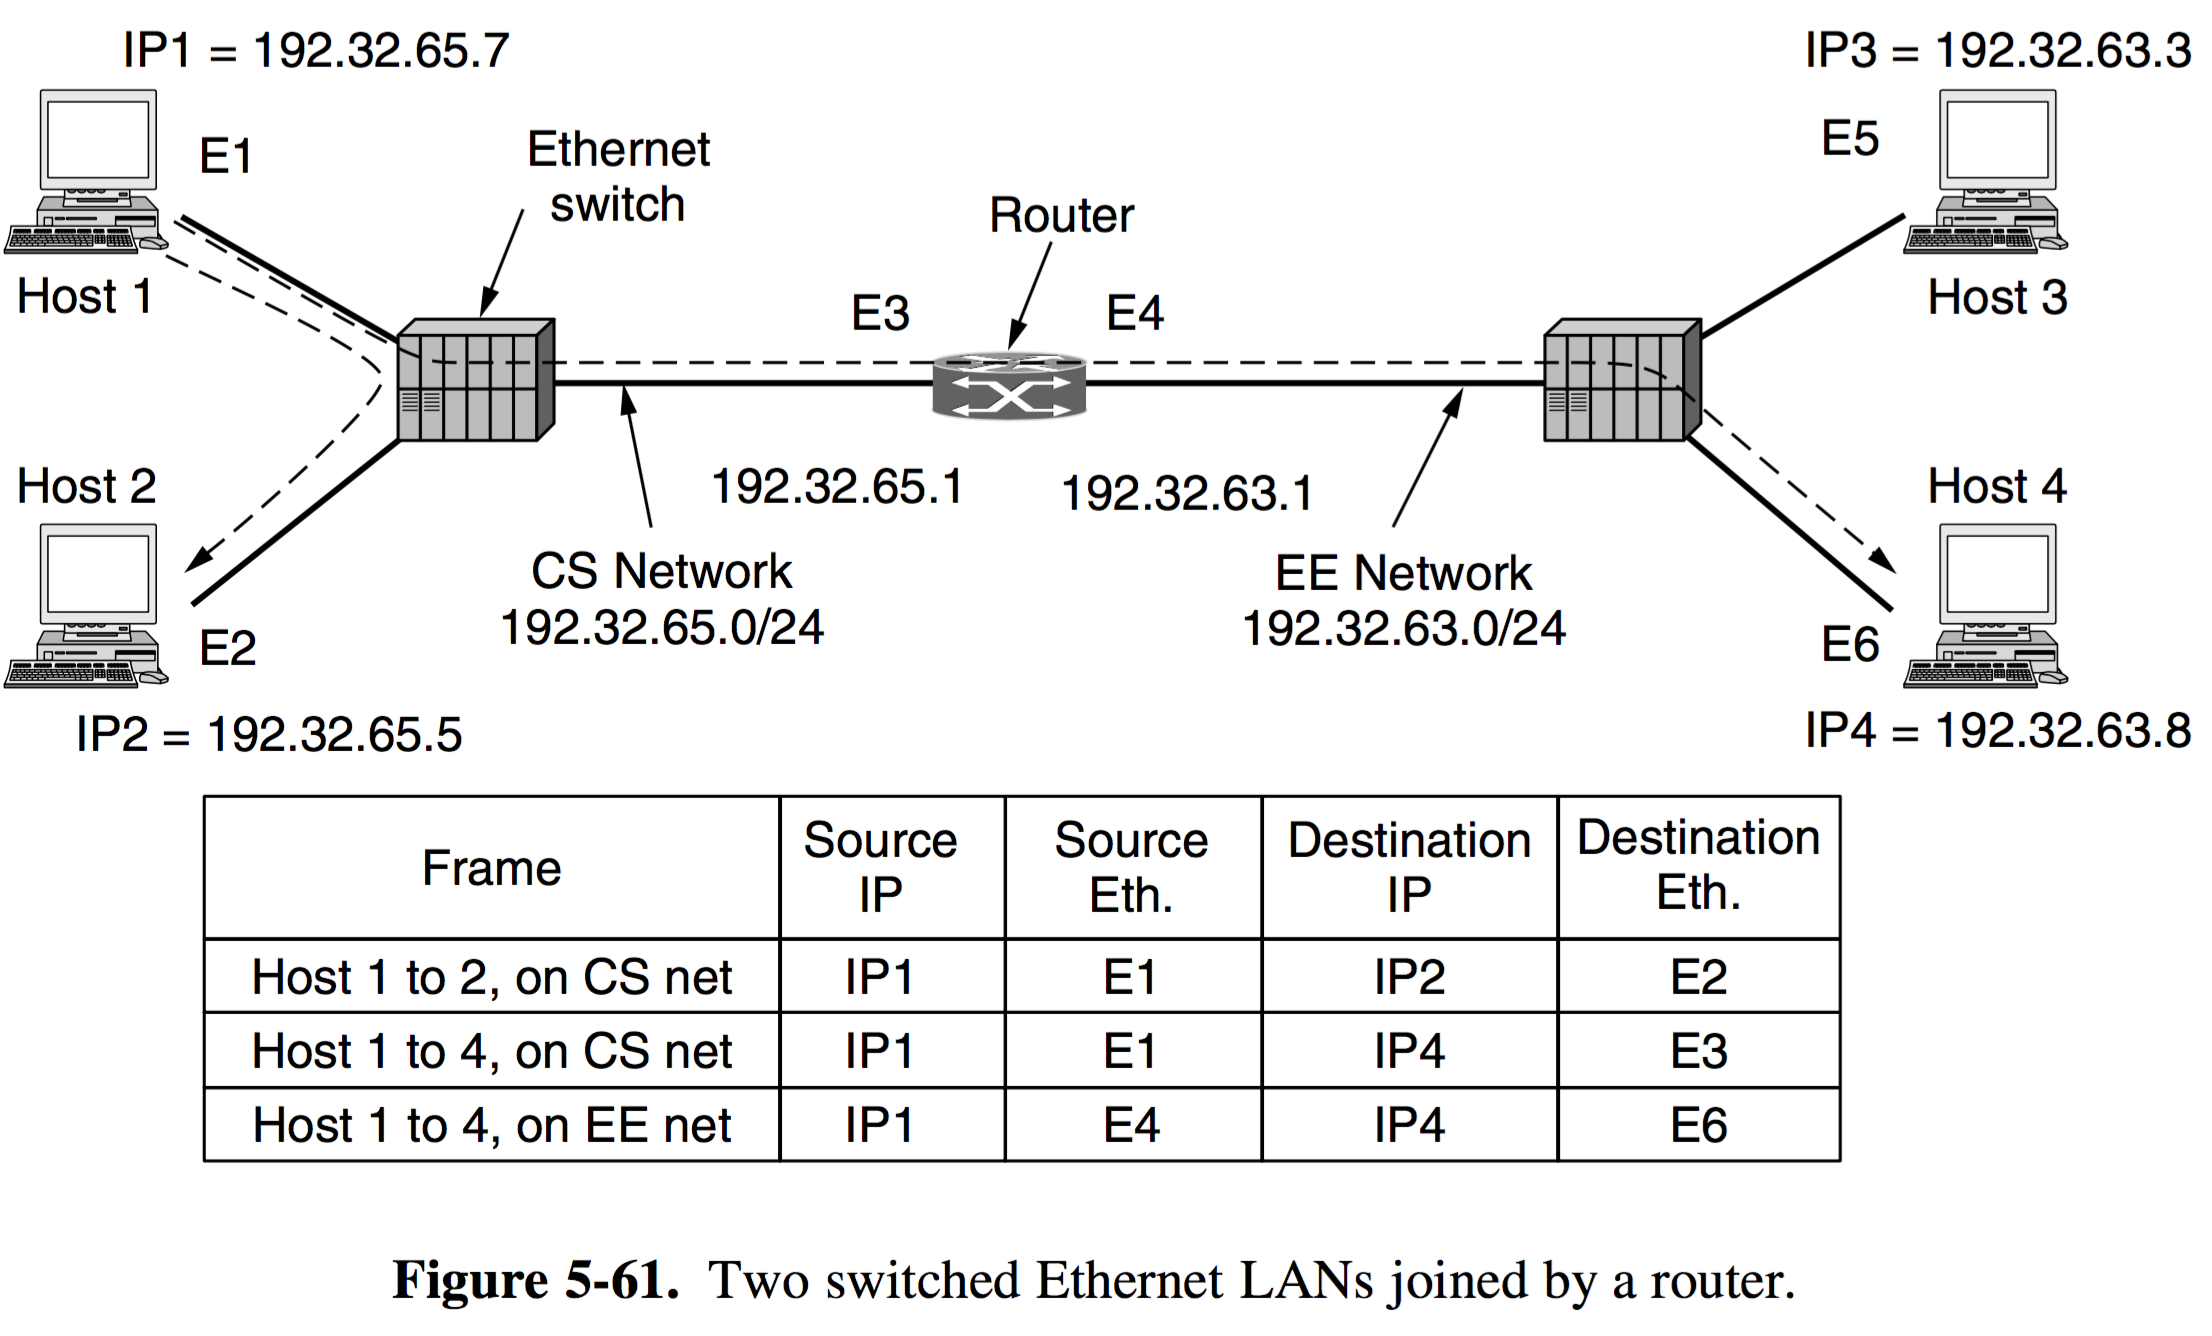
\includegraphics[width=9cm, height=6cm]{./imagenes/arp.png} 
		\end{center}

	\par Viendo la figura de arriba, supongamos que el \textit{host 1} quiere enviar un paquete al \textit{host 4} (192.32.63.8) en la red IE. El \textit{host 1} verá que la dirección IP de destino no está en la red CS. Sabe enviar todo ese tráfico fuera de la red al enrutador, el cual también se conoce como puerta de enlace predeterminada. Por convención, la puerta de enlace predeterminada es la dirección más baja en la red (198.31.65.1). Para enviar una trama al enrutador, el \textit{host 1} debe conocer de todas formas la dirección Ethernet de la interfaz del enrutador en la red CS. Para descubrirla envía una difusión ARP para 198.31.65.1, a partir de la cual aprende E3. Después envía la trama. Los mismos mecanismos de búsqueda se utilizan para enviar un paquete de un enrutador al siguiente, a través de una secuencia de enrutadores en una ruta de Internet.
	
	\par Cuando la placa de red de Ethernet del enrutador recibe esta trama, entrega el paquete al software IP. Sabe con base en las máscaras de red que el paquete se debe enviar a la red IE, en donde alcanzará al \textit{host 4}. Si el enrutador no conoce la dirección Ethernet para el \textit{host 4}, entonces usará ARP de nuevo. Las direcciones Ethernet cambian con la trama en cada red, mientras que las direcciones IP permanecen constantes (puesto que indican las terminales a través de todas las redes interconectadas).
	
%Lista
\subsection{OSPF: un protocolo de enrutamiento de puerta de enlace interior}
	\par Internet se compone de una gran cantidad de \textbf{Sistemas Autónomos}. Cada uno de ellos es manejado por una organización diferente y puede usar su propio algoritmo interno de enrutamiento. Un algoritmo de enrutamiento dentro de un sistema autónomo se llama \textbf{protocolo de puerta de enlace interior (IGP)}; un algoritmo para enrutamiento entre sistemas autónomos se llama protocolo de \textbf{puerta de enlace exterior (EGP)}.

	\par El protocolo de puerta de enlace interior original en internet era un protocolo de vector de distancia (\textit{RIP}). Fue reemplazado en 1979 por un protocolo de estado de enlace. Luego en 1988 se definió un sucesor llamado OSPF (\textbf{Open Shorted Path First}), que se volvió una norma en 1990. Ahora la mayoría de vendedores de enrutadores lo apoyan.
	
	\par OSPF tenía una larga lista de requerimientos por cumplir. El algoritmo se tenía que apoyar en una variedad de métricas de distancia como distancia física, retardo, etc. Tenía que ser un algoritmo dinámico que se adaptara rápida y automáticamente a los cambios en la topología. Debía apoyar el enrutamiento con base en el tipo de servicio. El nuevo protocolo tenía que dirigir el tráfico en tiempo real de una manera y el resto del tráfico de otra.
	
	\par El nuevo protocolo tenía que balancear la carga, dividiéndola en líneas múltiples. La mayoría de los protocolos anteriores enviaba todos los paquetes por la mejor ruta, incluso si había dos rutas buenas.

	\par Se necesitaba apoyo para los sistemas jerárquicos. Había que tratar con enrutadores que se conectan a internet por medio de un túnel.

	\par OSPF soporta tres tipos de conexiones y redes:

		\begin{enumerate}
			\item Las líneas punto a punto exactamente entre dos enrutadores.
			\item Redes de multiacceso con difusión (la mayoría de las LAN).
			\item Redes de multiacceso con muchos enrutadores, cada uno de los cuales se puede comunicar directamente con los otros.
		\end{enumerate}

	\par La siguiente figura muestra un sistema autónomo con los tres tipos de redes. En ella se omiten los hosts, ya que en general no desempeñan ningún papel en OSPF.

		\begin{center}
			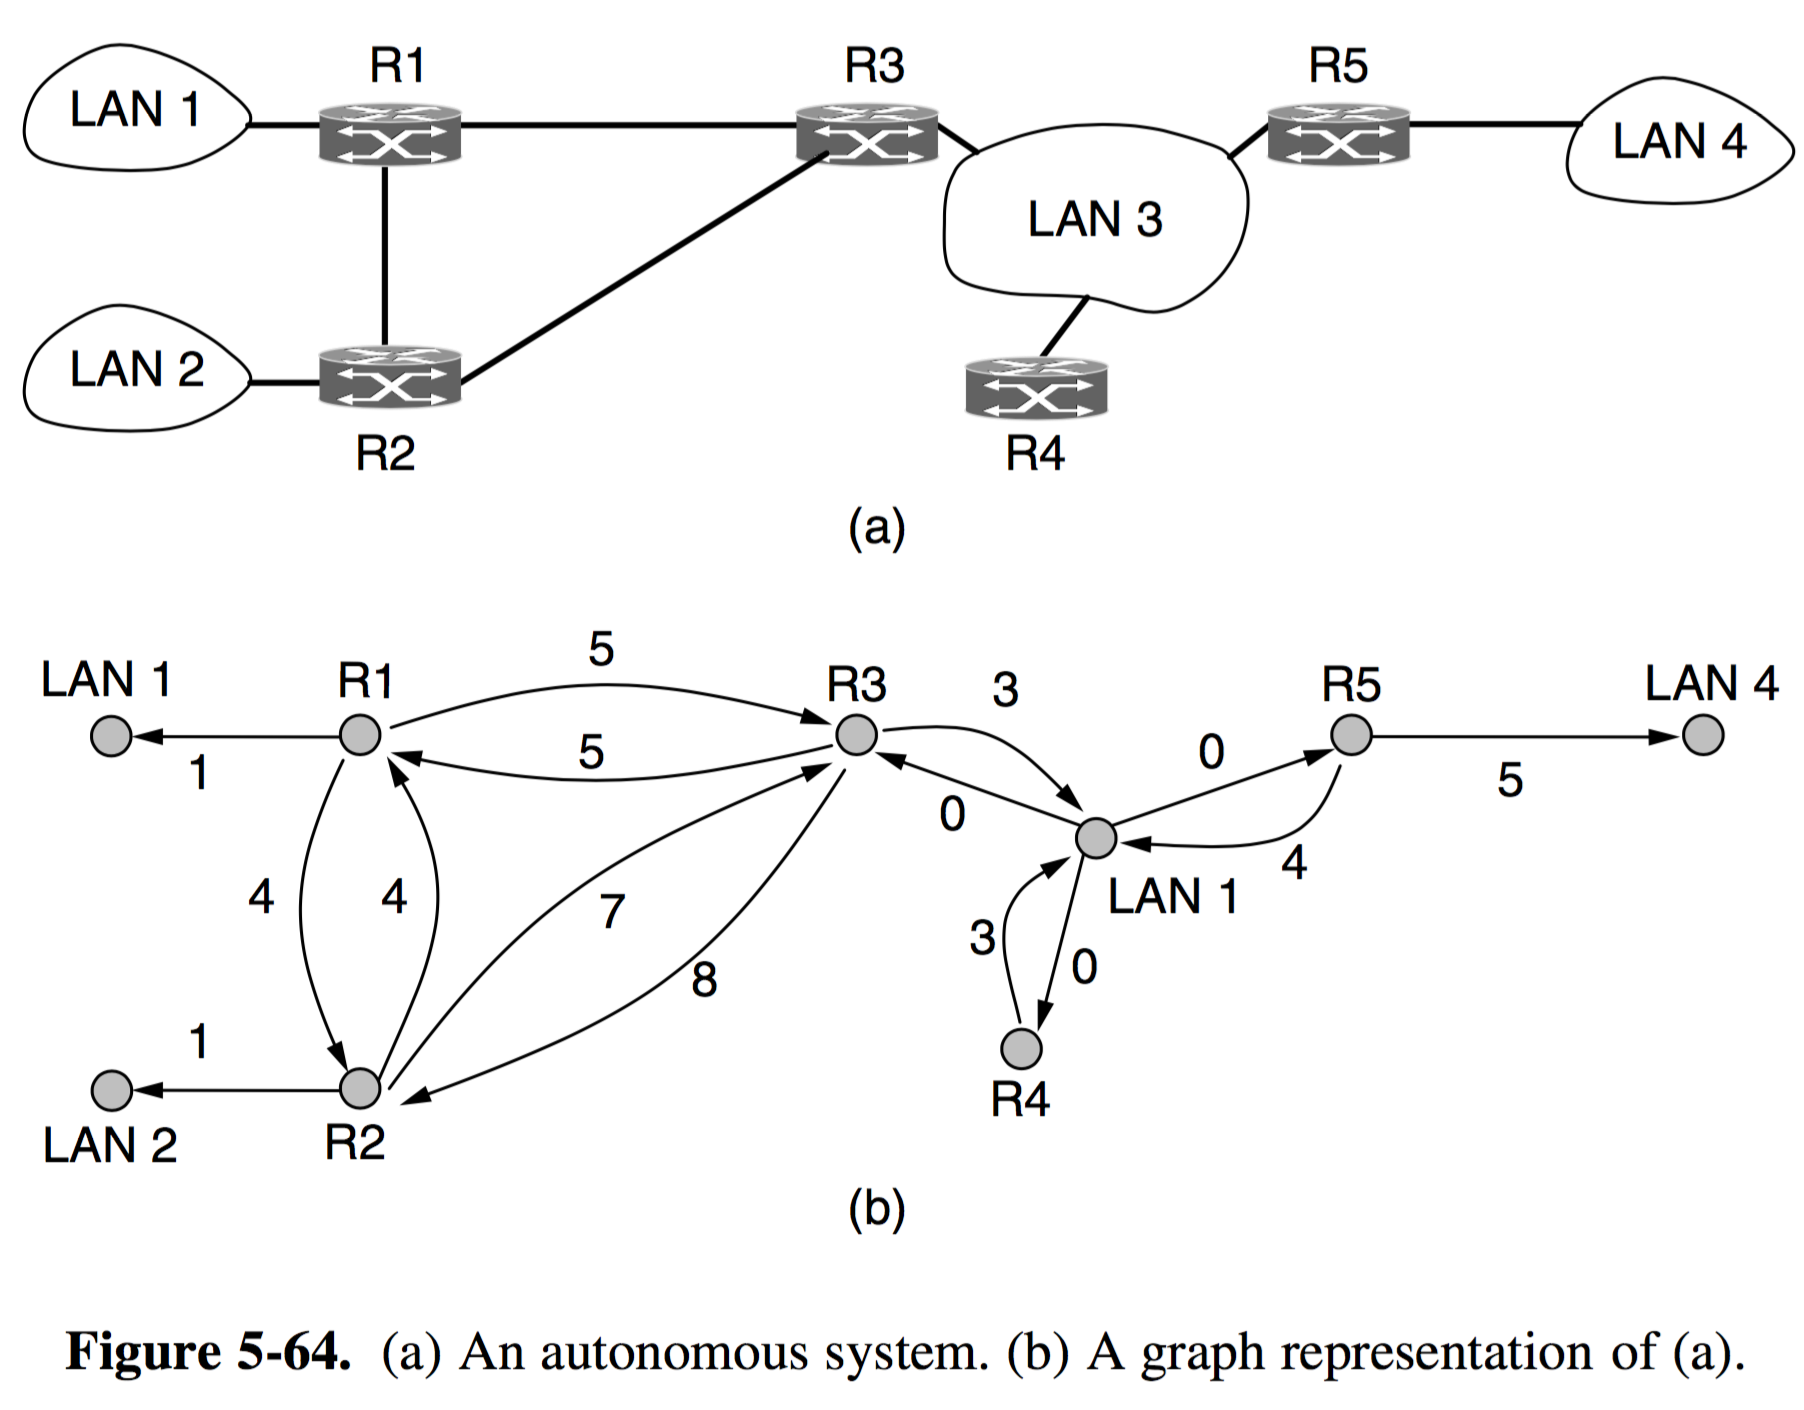
\includegraphics[width=8cm, height=5cm]{./imagenes/ospf.png} 
		\end{center}

	\par OSPF abstrae la topología en un \textbf{grafo dirigido} en el que a cada arco se asigna un costo (distancia, retardo, etc.). Una conexión \textit{punto-punto} entre dos enrutadores se representa por un par de arcos, uno en cada dirección, donde sus pesos pueden ser diferentes. Una red de multiacceso de difusión se representa con un nodo
para la red en sí, más un nodo para cada enrutador. Los arcos desde el nodo de la red a los enrutadores tienen peso 0, sin embargo son importantes puesto que sin ellos no habrá una ruta a través de la red.

	\par Luego de la construcción del grafo se utiliza al algoritmo de \textit{Dijkstra} para hacer que cada enrutador calcule la ruta más corta desde sí mismo hacia todos los demás nodos. Se pueden encontrar varias rutas que sean igual de cortas. En este caso, OSPF recuerda el conjunto de rutas más cortas y, durante el envío de paquetes, el tráfico se divide entre ellas. Este proceso ayuda a balancear la carga y se conoce como ECMP (\textbf{Equal Cost MultiPath}).

	\par Muchos de los sistemas autónomos (AS) en Internet son grandes por sí mismos y nada sencillos de administrar. Para trabajar a esta escala, OSPF permite dividir un AS en áreas numeradas, en donde un área es una red o un conjunto de redes contiguas y cada área puede contener varias redes dentro de sí misma. Las áreas no se traslapan, algunos enrutadores no necesitan pertenecer a ningún área. Los enrutadores que están totalmente dentro de un área se llaman \textbf{enrutadores internos}.

	\par Cada Sistema Autónomo tiene un área de \textbf{red dorsal}, llamada área 0. Los enrutadores en esta área se llaman \textbf{enrutadores dorsales}. Todas las áreas se conectan a la red dorsal, posiblemente mediante túneles, de modo que es posible ir desde cualquier área en el AS a cualquier otra área en el AS mediante la red dorsal. En el grafo, un túnel se representa como otro arco más con un costo. Al igual que con otras áreas, la topología de la red troncal no es visible fuera de esta.

	\par Cada enrutador que se conecta a dos o más áreas se llama \textbf{enrutador de borde de área} (\textit{EBA}) y es parte de la red dorsal y a la vez de una o más áreas.

	\par El \textbf{enrutador de borde de sistema autónomo} (\textit{EBSA}) inyecta en el área rutas a destinos externos en otros AS. Las rutas externas aparecen como destinos que pueden ser alcanzados vía un EBSA con algún costo. Una ruta externa puede ser inyectada a uno o más EBSA.

	\begin{center}
			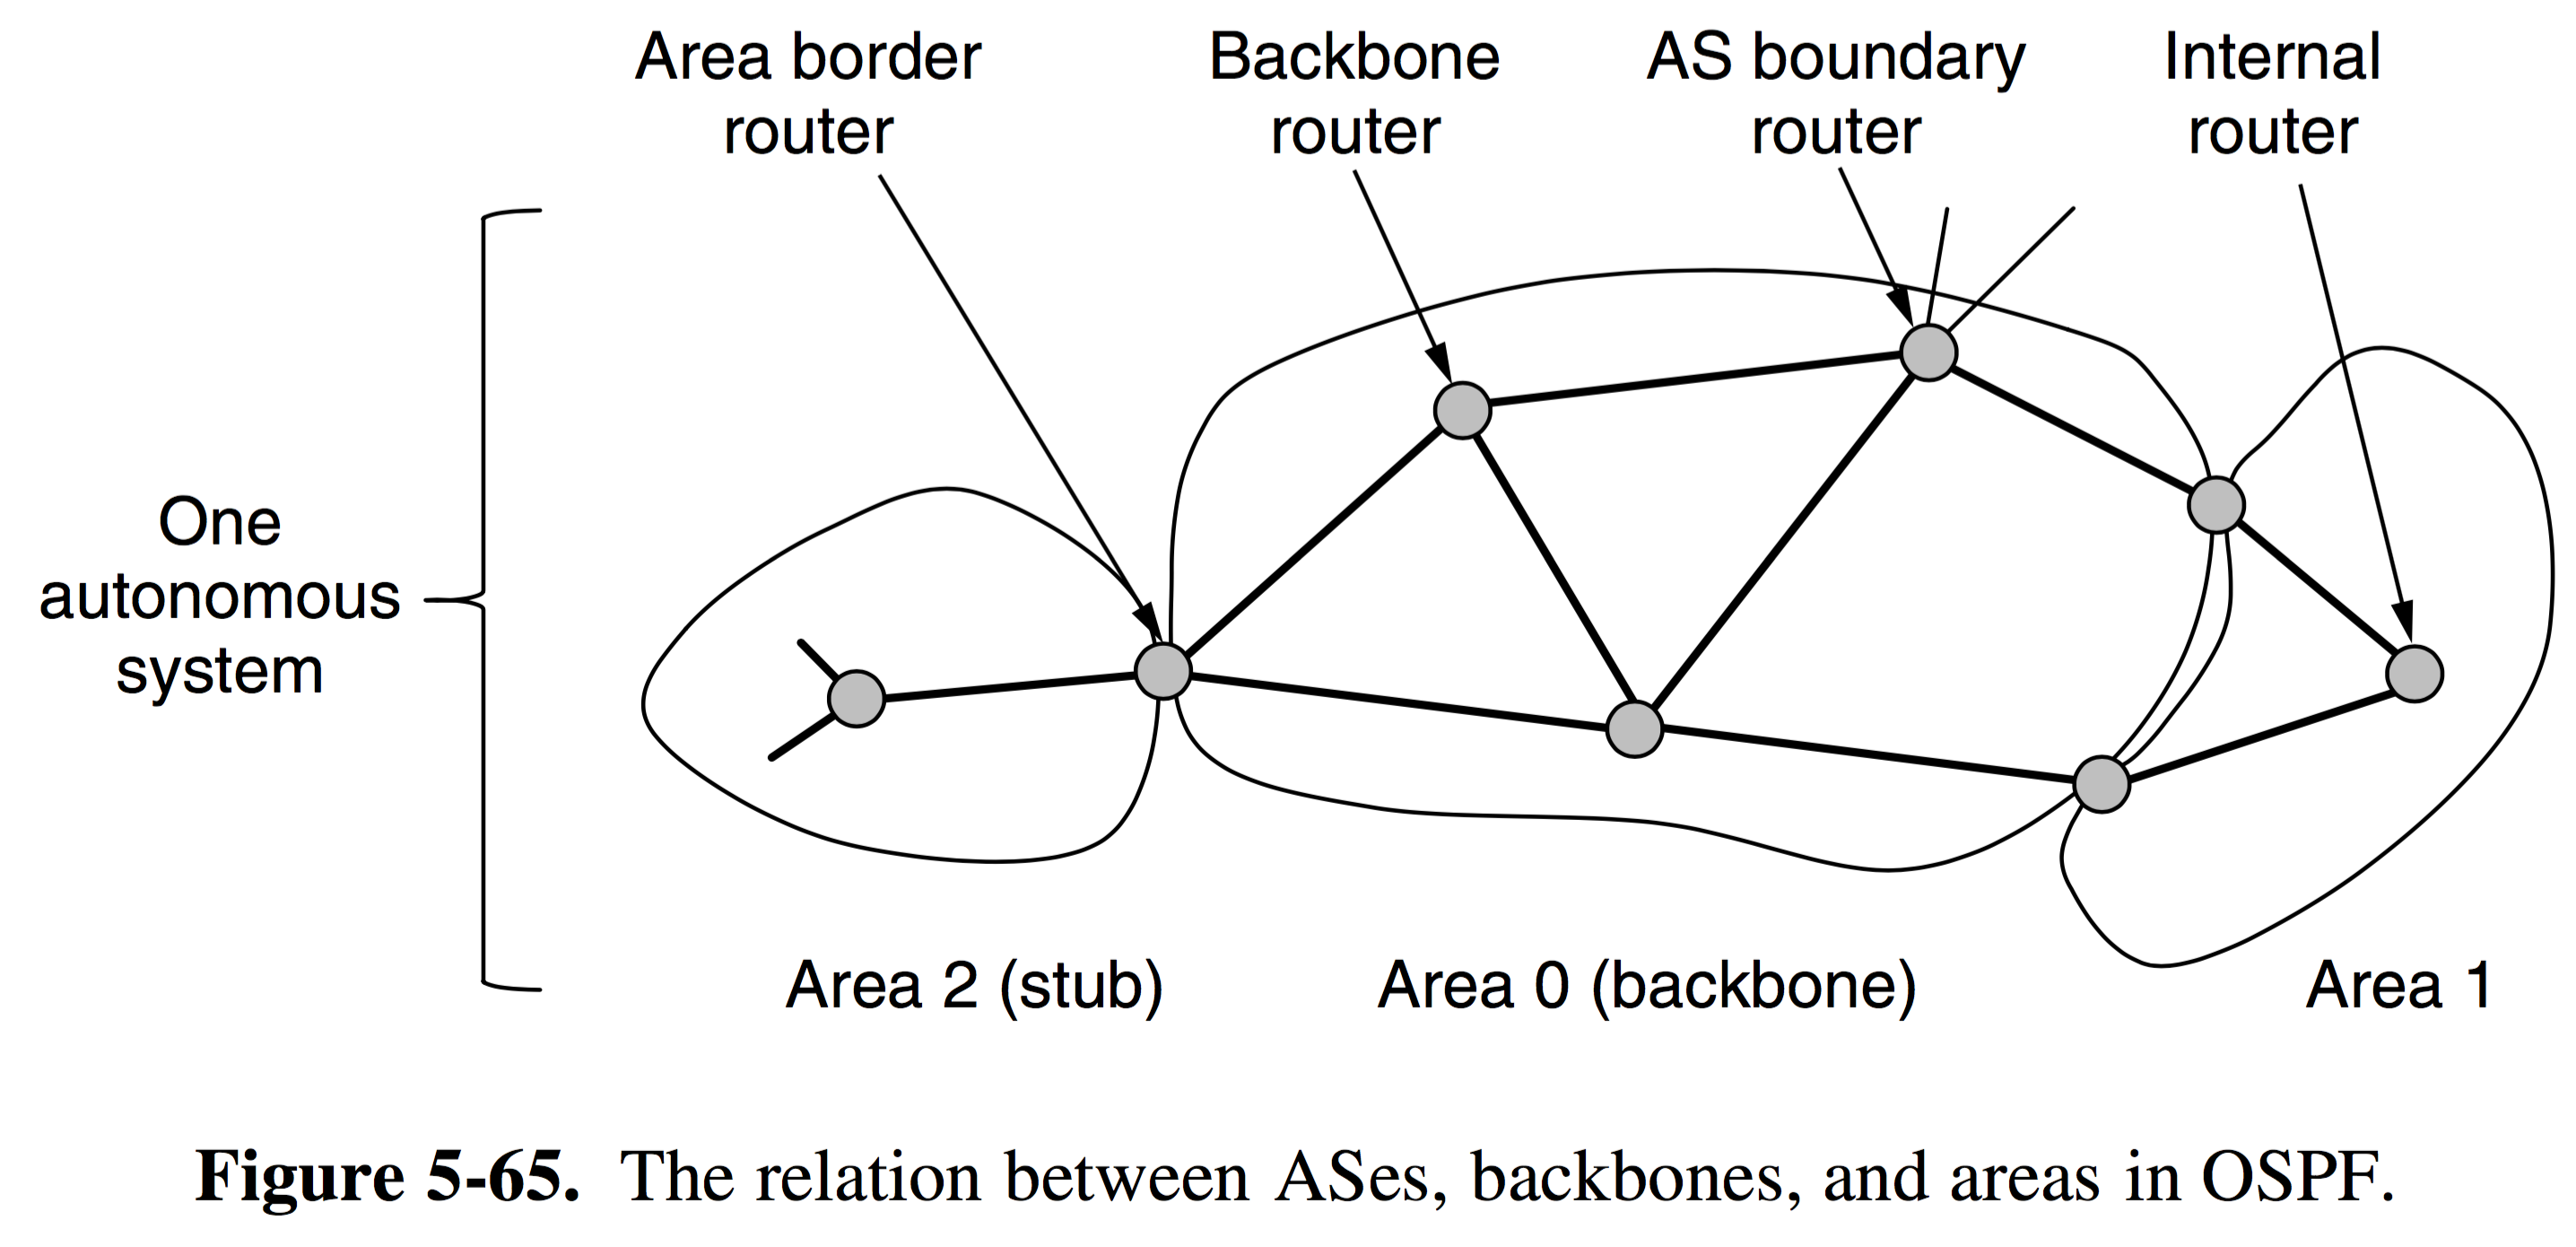
\includegraphics[width=9cm, height=5cm]{./imagenes/ospf2.png} 
		\end{center}
		
	\par Los EBA resumen información de enrutamiento que han aprendido de un área y la hacen disponible en sus avisos de estado de enlace que envían a las otras áreas. Un EBA recibe mensajes de estado de enlace de todos los enrutadores de una de sus áreas A y entonces determina el costo de alcanzar cada red de A. Cuando un EBA envía avisos de estado de enlace a la red dorsal, avisa de los costos de alcanzar las redes del área A, como si estas redes estuvieran directamente conectadas al EBA, esto permite que todos los enrutadores del área dorsal aprendan el costo de alcanzar todas las redes del área A. Cuando un EBA envía avisos de estado de enlace a su red no dorsal, avisa de los costos a alcanzar todas las redes de las otras áreas (no dorsal). Luego todos los enrutadores aprenden a alcanzar todas las redes en el dominio.
	
	\par Cuando se ejecuta OSPF los enrutadores dentro de un área ejecutan el protocolo de estado de enlace, hay paquetes \textbf{Hello}. Los enrutadores dentro de un área intercambian mensajes de estado de enlace periódicamente usando inundación. Estos enrutadores también envían estos mensajes cuando una línea se cae, regresa o su costo cambia. Los mensajes de estado de enlace de enrutadores que no son EBA no dejan el área en el que se originan. Los enrutadores internos a un área no van a conocer detalles acerca de la topología de otras áreas.

	\par Dentro de un área cada enrutador tiene la misma \textbf{base de datos de estado de enlace} (\textit{BDEE}) y ejecuta el mismo algoritmo de la ruta más corta. Su trabajo principal es calcular el camino más corto desde sí mismo a cualquier otro enrutador de su área y red en el AS entero. Un EBA necesita las bases de datos de estado de enlace para todas las áreas a las cuales está conectado y debe correr el algoritmo de Dijkstra para cada área separadamente.


\subsection{BGP: el protocolo de enrutamiento de Puerta de Enlace Exterior}
	\par Los enrutadores de protocolo de puerta de enlace exterior tienen que 
	preocuparse en gran parte por la política. Muchas veces se quiere mantener las 
	políticas privadas; porque los Sistemas Autónomos (SA) compiten entre sí (ej: PSI 
	competidores).	
	\par Las políticas típicas implican consideraciones políticas, de seguridad, o 
	económicas. Algunos ejemplos de posibles restricciones de enrutamiento son:
		\begin{enumerate}
			\item  No transportar tráfico comercial en la red educativa.
			\item Nunca enviar tráfico del Pentágono por una ruta a través de Irak.
			\item Usar TeliaSonera en vez de Verizon porque es más económico.
			\item No usar AT and T en Australia porque el desempeño es pobre.
			\item El tráfico que empieza o termina en Apple no debe transitar por Google.
		\end{enumerate}

	\par Para enrutamiento inter SA encontrar un camino óptimo es prácticamente 
	imposible. Cada SA corre su propio protocolo interno y usa cualquier esquema para 
	asignar métricas a los caminos. Es imposible calcular costos de caminos 
	significativos para caminos que cruzan varios SA.
	\par Enrutamiento inter SA solo avisa alcanzabilidad, por lo tanto, a lo más puedo 
	tener caminos de SA para ir de un origen a un destino.
	
	\par Para el enrutamiento es necesario encontrar algún camino de SA para el destino 
	deseado que es libre de ciclos. Además los caminos deben respetar las políticas de 
	los SA a lo largo del camino. Donde una política significan reglas que se refieren a 
	preferencias de enrutamiento y a limitaciones de enrutamiento.
   \par Los PPEE suelen implementarse sobre enrutadores de borde de sistema 
   autónomos (EBSA), los cuales tienen que hacer una elección de varias rutas a un 
   destino; va a elegir la mejor de acuerdo con sus propias políticas locales y esta va a 
   ser la ruta que avisa. Además le dice a sus vecinos para cada destino, el camino 
   exacto que está usando.
	\par Muchos PSI existen solo para proveer servicios a consumidores (ej: redes 
	hogareñas). Otros PSI ofrecen algo parecido a un servicio dorsal interconectando 
	otros PSI y a veces grandes corporaciones. A menudo varios proveedores se 
	conectan entre sí como un punto único de compañerismo.


\chapter{LA CAPA DE TRANSPORTE}
\par Junto con la capa de red, la capa de transporte es el corazón de la jerarquía de 
protocolos. La capa de red provee una entrega de paquetes punto a punto mediante 
el uso de datagramas o circuitos virtuales. La capa de transporte se basa en la capa 
de red para proveer transporte de datos de un proceso en una máquina de origen a 
un proceso en una máquina de destino, con un nivel deseado de confiabilidad que es 
independiente de las redes físicas que se utilizan en la actualidad. Ofrece las 
abstracciones que necesitan las aplicaciones para usar la red. Sin esta capa, todo el 
concepto de protocolos por capas tendría muy poco sentido.


\section{El servicio de transporte}
\subsection{Servicios que se proporcionan a las capas superiores}
\par La capa de transporte (CT), al igual que a capa de red, provee:
	\begin{itemize}
		\item un servicio confiable a sus usuarios (orientado a la conexión)
		\item un servicio eficiente a sus usuarios (no orientado a la conexión)
	\end{itemize}
	
\par La capa de transporte se ejecuta por completo en las máquinas de los usuarios 
(hosts). El software/hardware de la capa de transporte se llama \textbf{entidad de 
transporte}.

\par Si en una red sin conexión se pierden paquetes, la entidad de transporte puede 
detectar el problema y compensarlo mediante el uso de retransmisiones. Si, en una 
red orientada a conexión, se termina la conexión de manera abrupta, la entidad puede 
establecer una nueva conexión de red con la entidad de transporte remota.
\par El servicio de transporte se ofrece a programadores y usuarios, debe ser fácil de 
usar y no debe exponer cuestiones internas (retransmisiones, fragmentación, etc.)

	\begin{center}
	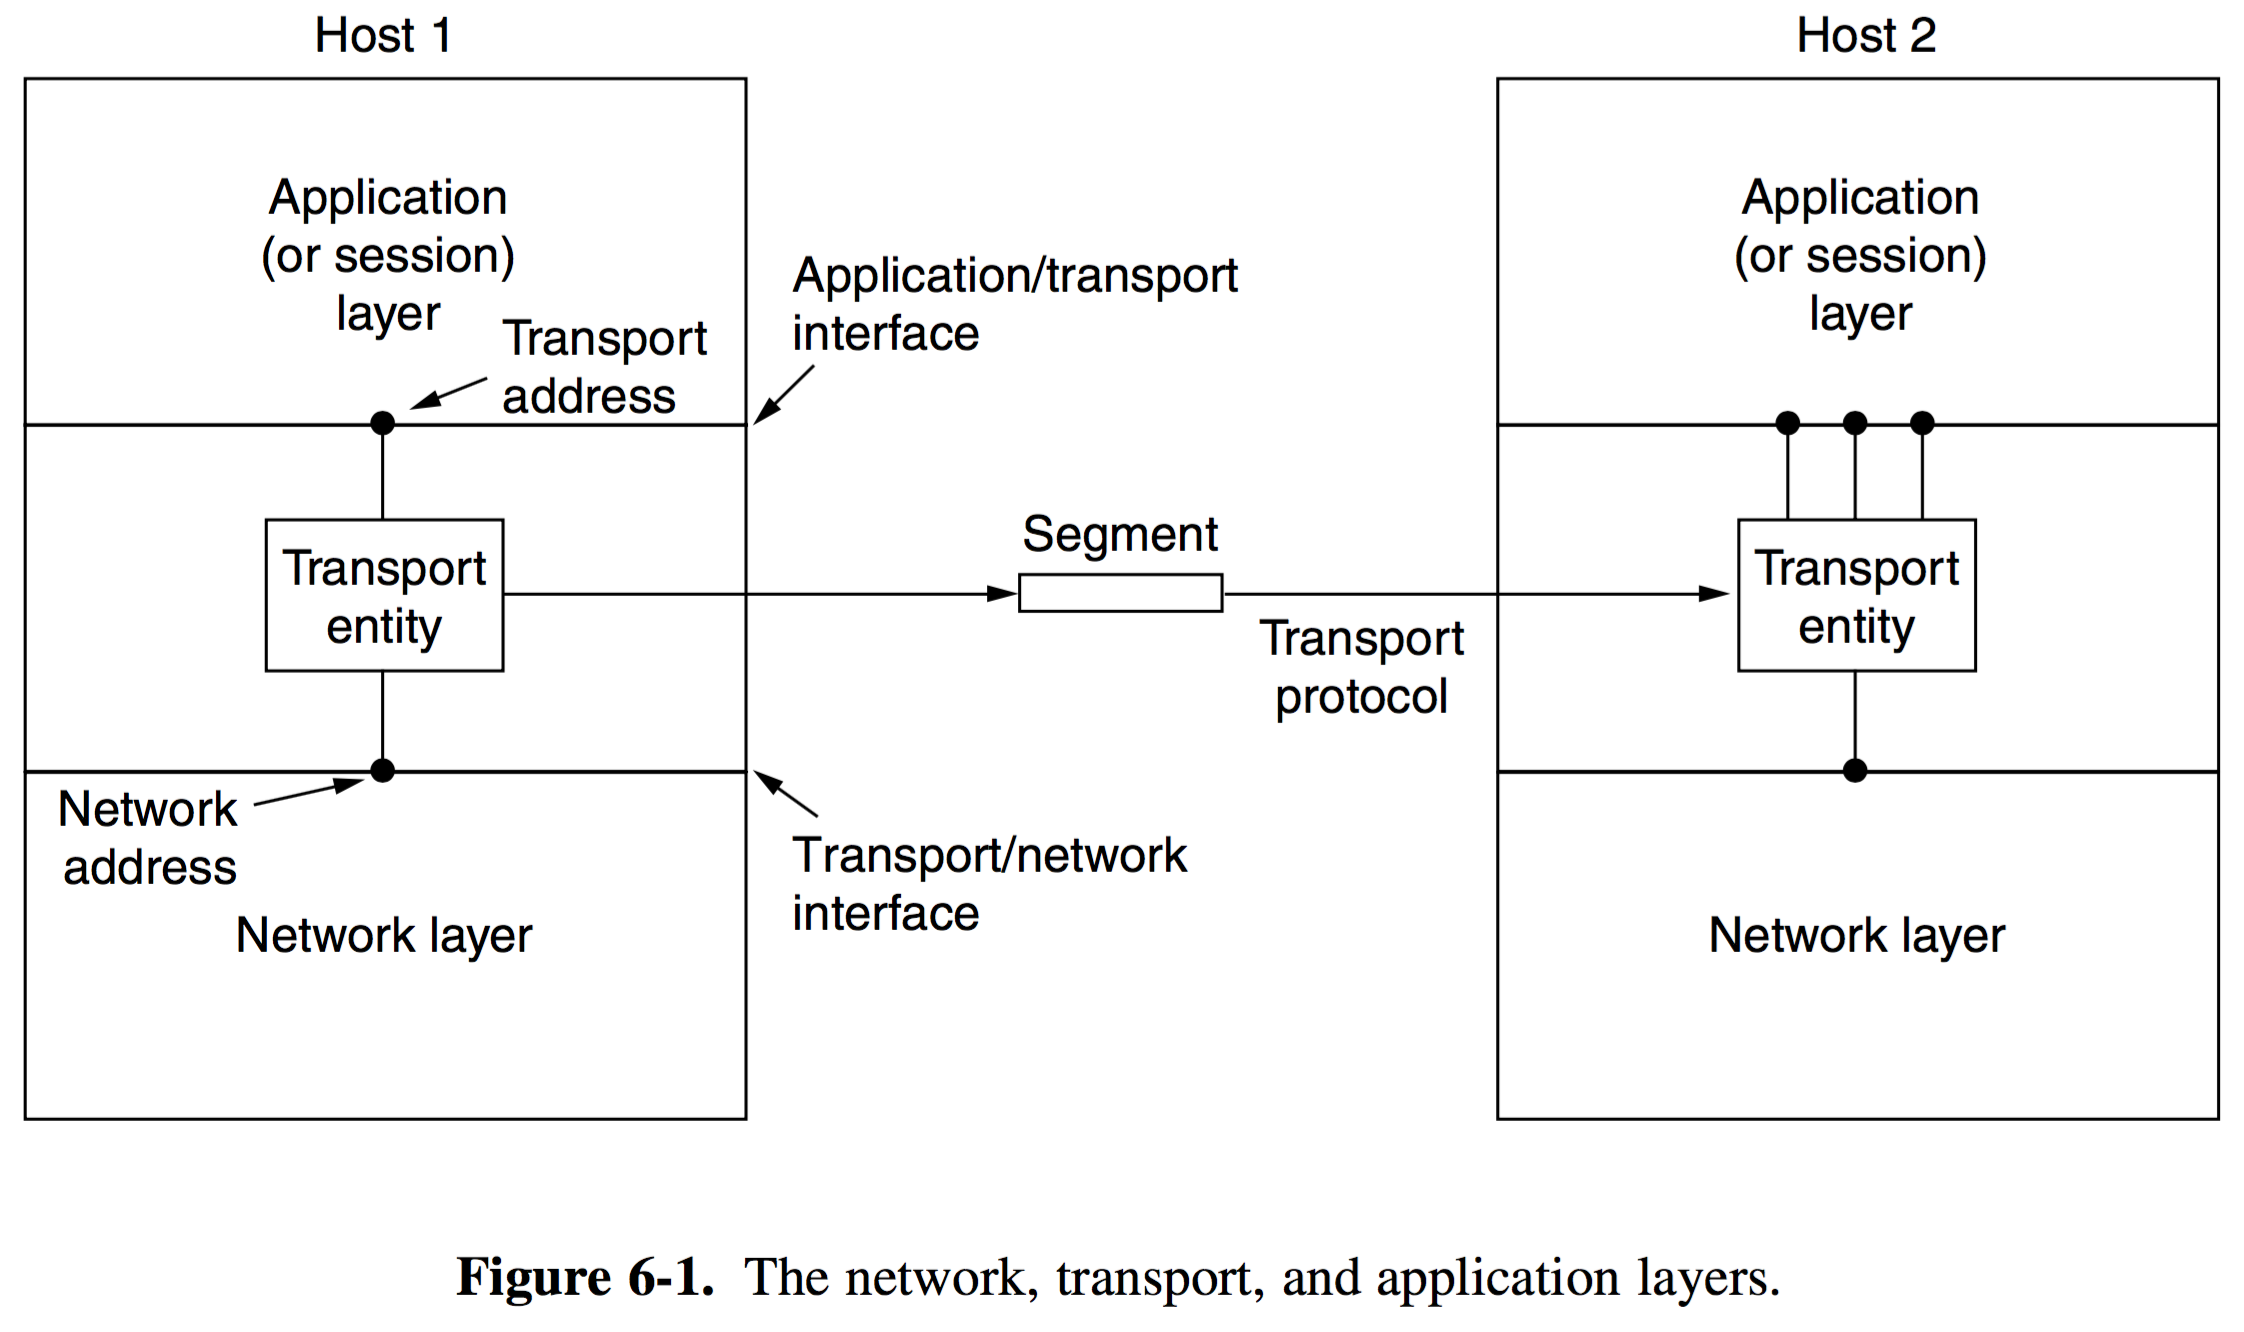
\includegraphics[width=8cm, height=5cm]{./imagenes/transporte.png} 
	\end{center}

\subsection{Primitivas del servicio de transporte}


\par Para permitir que los usuarios accedan al servicio de transporte, la capa de 
transporte debe proporcionar algunas operaciones a los programas de aplicación; es 
decir, una interfaz del servicio de transporte.

\begin{center}
	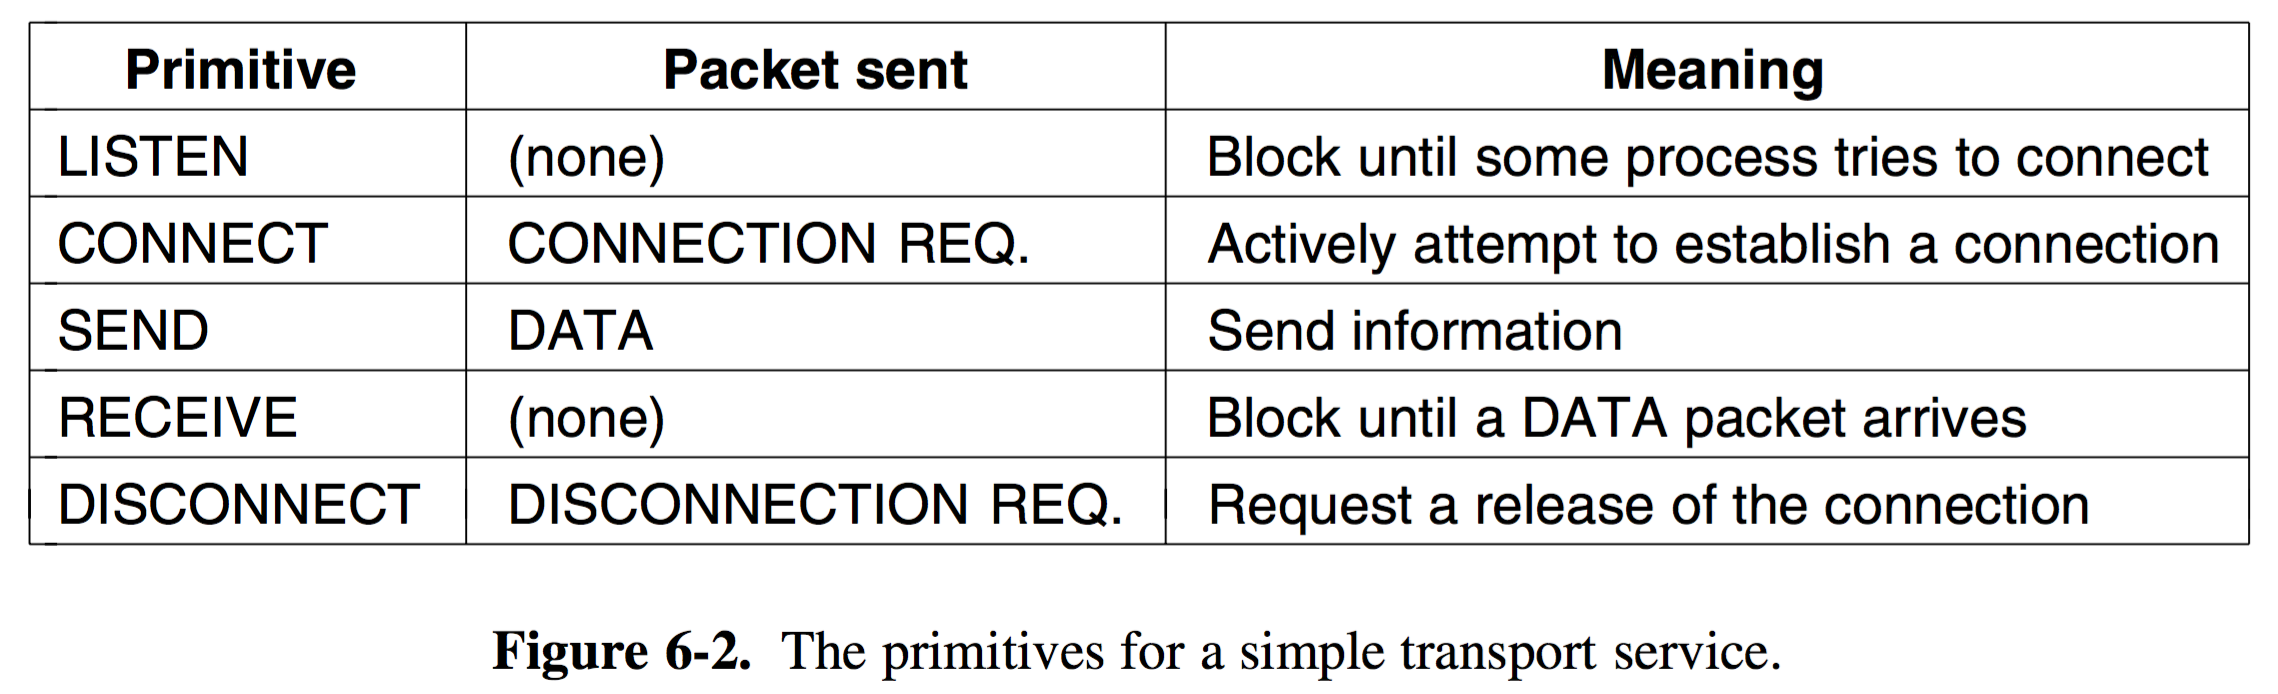
\includegraphics[width=11cm, height=5cm]{./imagenes/primitivas.png} 
\end{center}

\par Usaremos el término \textbf{segmento} para indicar los mensajes que se envían 
de una entidad de transporte a otra. Así, los segmentos (intercambiados por la capa 
de transporte) están contenidos en paquetes (intercambiados por la capa de red), y a 
su vez estos paquetes están contenidos en \textbf{tramas} (intercambiadas por la 
capa de enlace de datos).
\par Cuando llega una trama, la capa de enlace de datos procesa el encabezado de la 
trama y, si la dirección de destino coincide para la entrega local, pasa el contenido del 
campo de carga útil de la trama a la entidad de red. Esta úlltima procesa de manera 
similar el encabezado del paquete y después pasa el contenido de la carga útil del 
paquete a la entidad de transporte. 

\begin{center}
	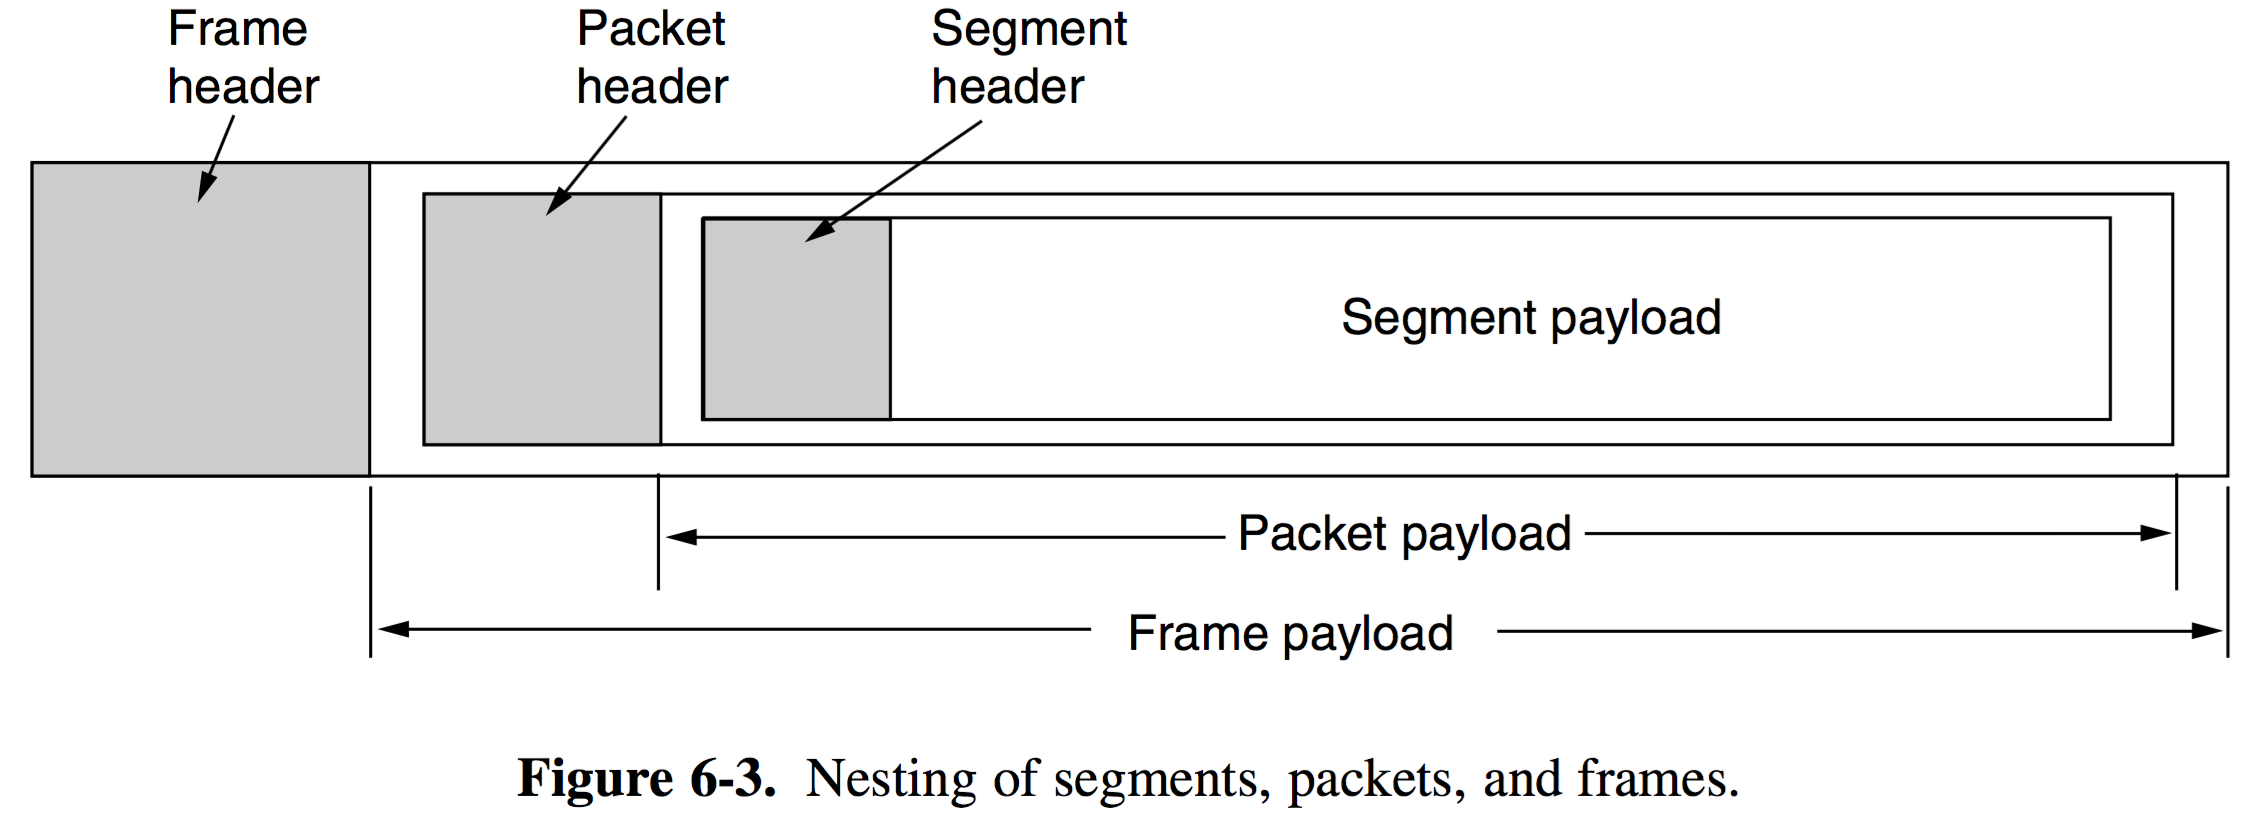
\includegraphics[width=8cm, height=4cm]{./imagenes/segmentos.png} 
\end{center}

\par Durante una conexión entre dos host se confirmará la recepción de cada 
paquete de datos enviado mediante las entidades de transporte, de manera 
transparente para los usuarios de transporte. De la misma forma, las entidades de 
transporte tienen que preocuparse por los temporizadores y las retransmisiones. Los 
usuarios de transporte no se enteran de ningún aspecto de esta mecánica. Para ellos 
una conexión es un conducto de bits confiable: un usuario mete bits en él y por arte 
de magia aparecen en el otro lado, con el mismo orden.

\par Veamos ahora un diagrama de estado para un esquema simple de manejo de 
conexiónes:

\begin{center}
	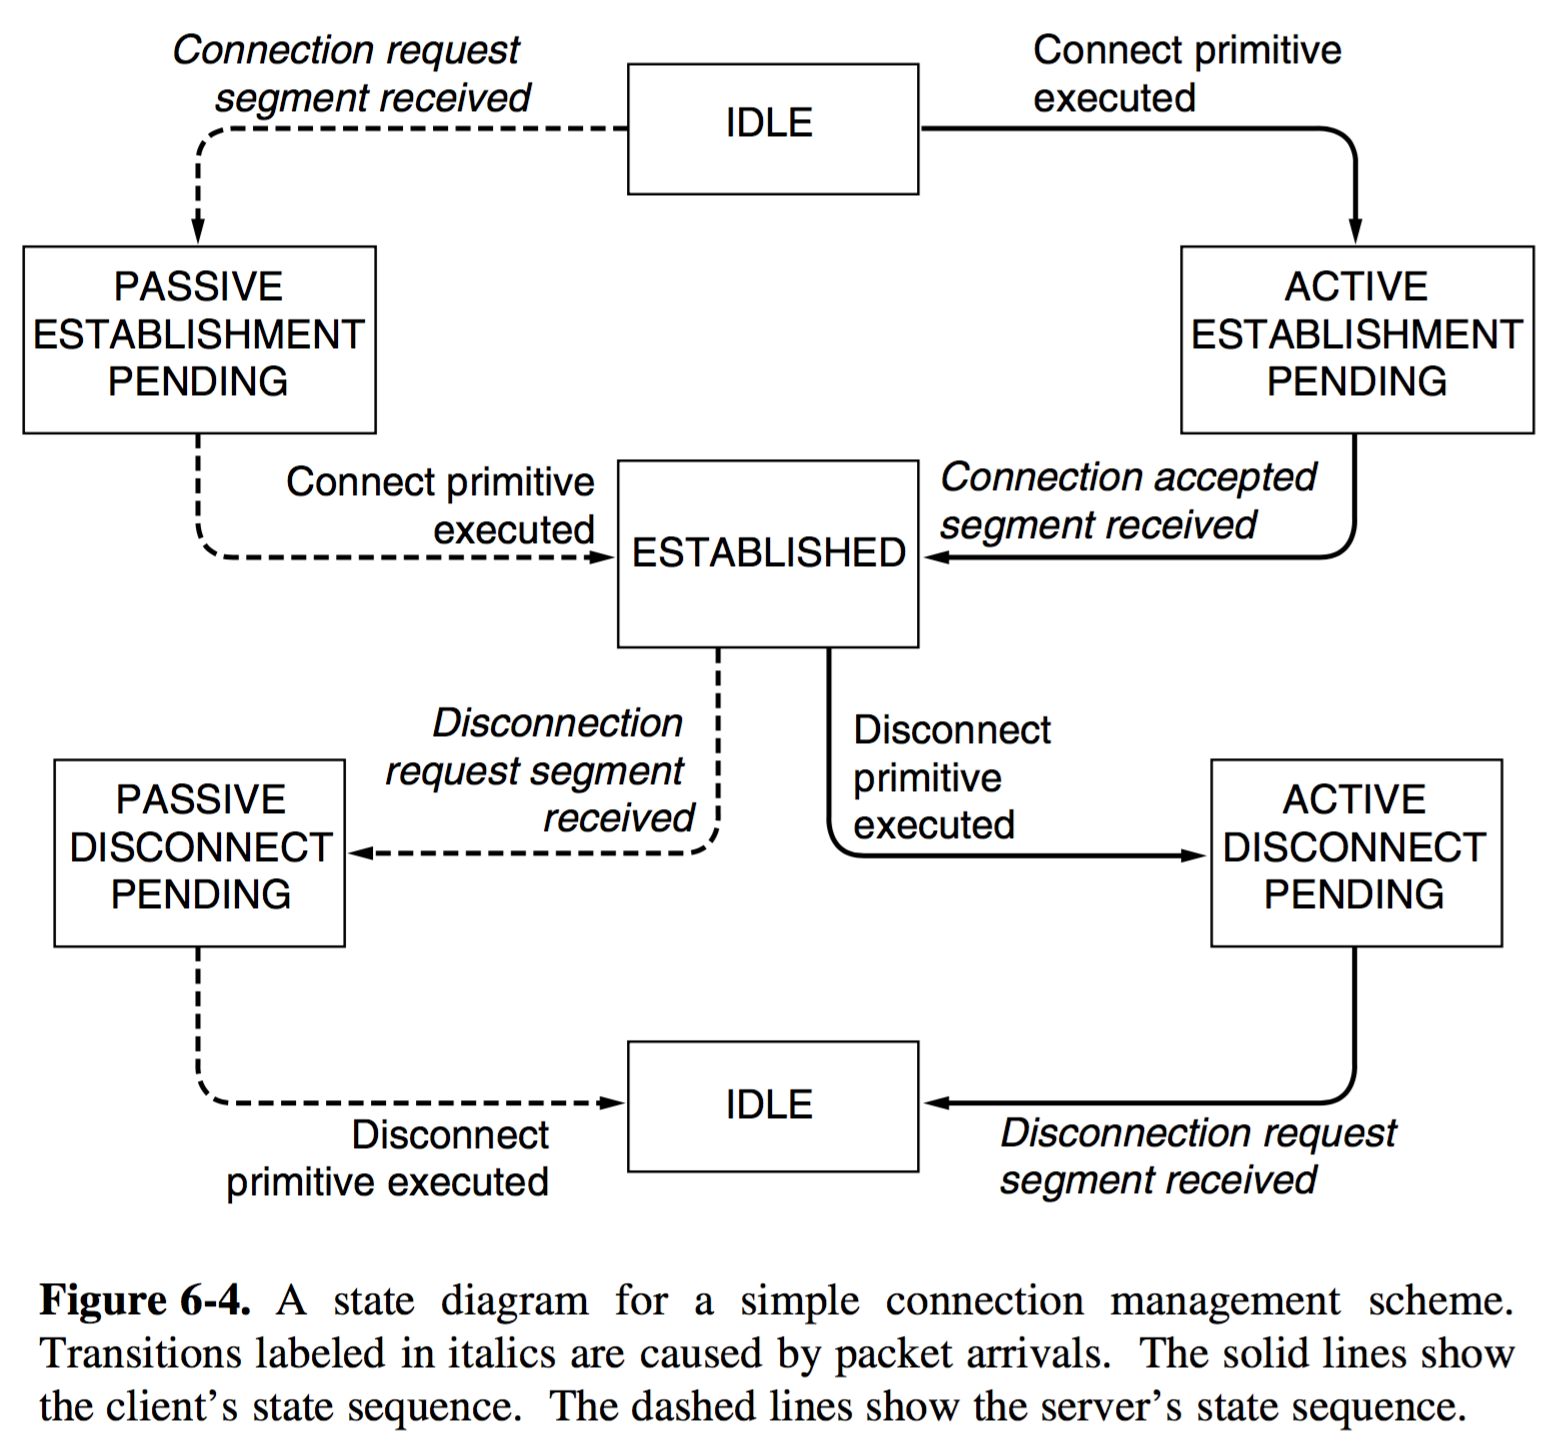
\includegraphics[width=11cm, height=7cm]{./imagenes/diagrama.png} 
\end{center}


\section{Elementos de los protocolos de transporte}
	\par El servicio de transporte se implementa mediante un \textbf{protocolo de 
transporte} entre las dos entidades de transporte. En la capa de transporte se requiere 
el direccionamiento explícito de los destinos, se requieren búferes y control de flujo.

\subsection{Direccionamiento}
\par Cuando un proceso de aplicación desea establecer una conexión con un proceso 
de aplicación remoto, debe especificar a cuáll se conectará. El método que se emplea 
por lo general es definir direcciones de transporte en las que los procesos puedan 
escuchar las solicitudes de conexión. En Internet, estos puntos terminales se 
denominan \textbf{puertos}. Usaremos el término genérico TSAP (Transport Service 
Access Point) para indicar un punto terminal específico en la capa de transporte. Los 
puntos terminales análogos en la capa de red (es decir, direcciones de capa de red) se 
llamen NSAP (Network Service Access Points). Las direcciones IP son ejemplos de 
NSAP.
\par Los procesos de aplicación,tanto clientes como servidores, se pueden enlazar por 
si mismos a un TSAP para establecer una conexión a un TSAP remoto. Estas 
conexiónes se realizan a través de NSAPs en cada host. Los TSAPs sirven para 
distinguir los múltiples puntos terminales de transporte que comparten un NSAP.

\begin{center}
	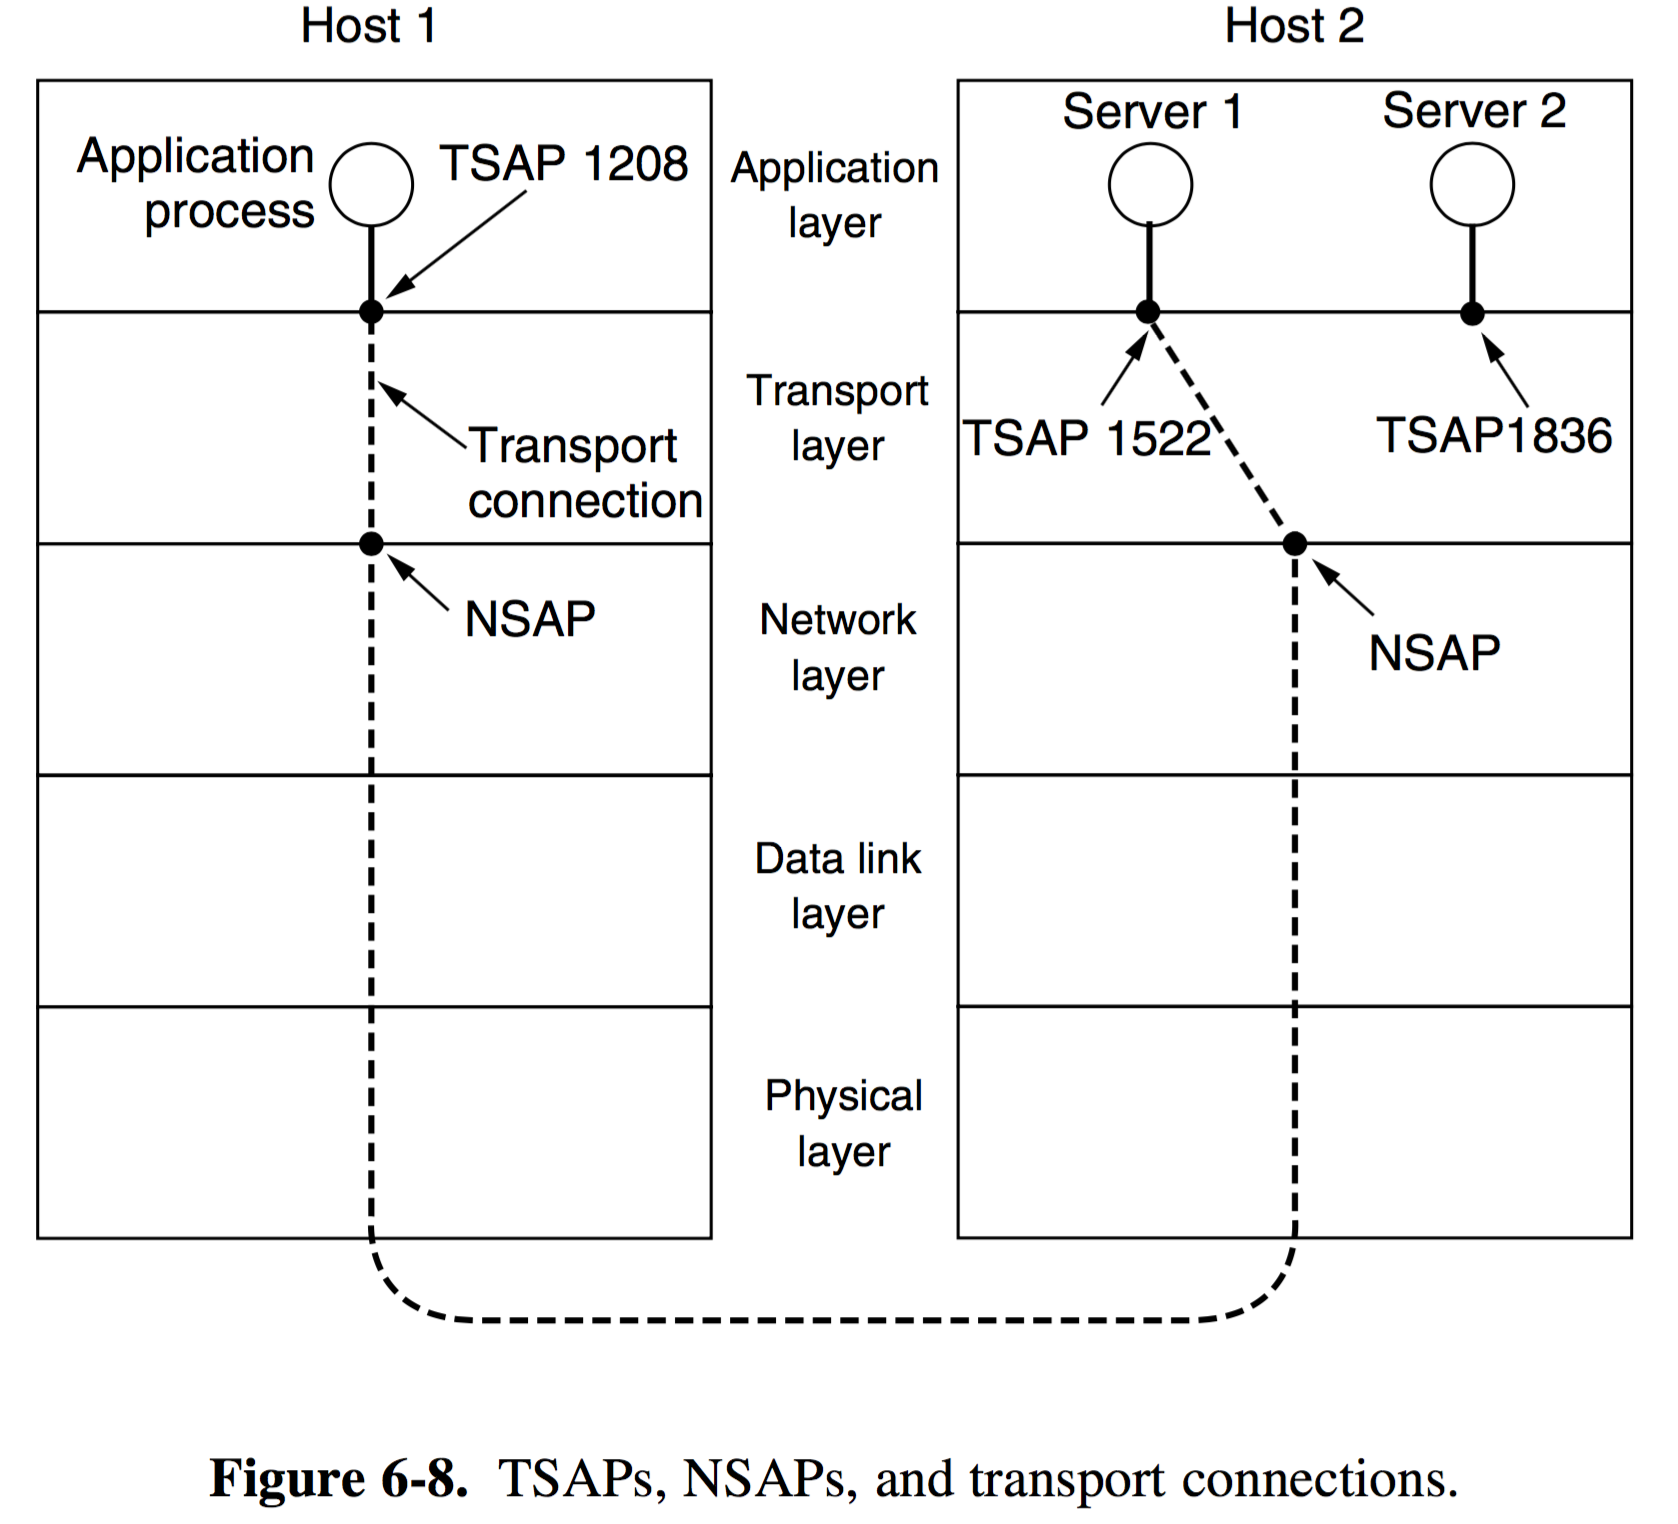
\includegraphics[width=6cm, height=5cm]{./imagenes/tsap.png} 
\end{center}

\par ¿Cómo sabe un proceso de usuario que un servidor \textbf{\textit{S}} está 
conectado a un determinado TSAP?

\begin{itemize}
	\item \underline{Solución 1:} una posibilidad es que S se ha estado conectando al 
	mismo TSAP durante años y gradualmente todos los usuarios de la red han 
	aprendido esto. En este modelo los servicios tienen direcciones TSAP estables que 
	se listan en archivos en lugares bien conocidos.
	\par Los procesos de usuario frecuentemente desean comunicarse con otros 
	procesos de usuario que solo existen durante un tiempo corto y no tienen una 
	dirección TSAP conocida por adelantado. En el caso de que hubiese muchos 
	procesos de servidor, la mayoría de los cuales se usaran pocas veces sería un 
	desperdicio tenerlos activados a todos escuchando en una dirección TSAP estable 
	todo el día.
	\item \underline{Solución 2:} un esquema alternativo en forma simplificada, es el 
	conocido como \textbf{protocolo inicial de conexión}. Cada máquina que desea 
	ofrecer servicios a usuarios remotos tiene un servidor de procesos especial que 
	actúa como 	proxy de los servidores de menor uso. Este servidor es llamado 
	\textit{inetd} en sistemas UNIX; el mismo escucha en un grupo de puertos al mismo 
	tiempo esperando una solicitud de conexión. Los usuarios potenciales de un 
	servicio comienzan por emitir una solicitud 	\textbf{CONNECT}, especificando la 
	dirección	TSAP del servicio que desean, si no hay ningún servidor esperándolos, 
	consiguen una conexión al servidor de procesos.
	 \par Tras obtener la solicitud entrante el servidor de procesos genera el servidor 
	 solicitado, permitiéndole heredar la conexión con el usuario existente. El nuevo 
	 servidor entonces hace el trabajo requerido, mientras que el servidor de procesos 
	 retorna a escuchar solicitudes nuevas.
	\par Hay muchas situaciones en las que los servicios existen independientemente 
	del servidor de procesos. Por ejemplo, un servidor de archivos necesita operar en un 
	hardware especial (una máquina con un disco) y no puede crearse simplemente 
	sobre la marcha cuando alguien quiere comunicarse con él.
	
	\begin{center}
	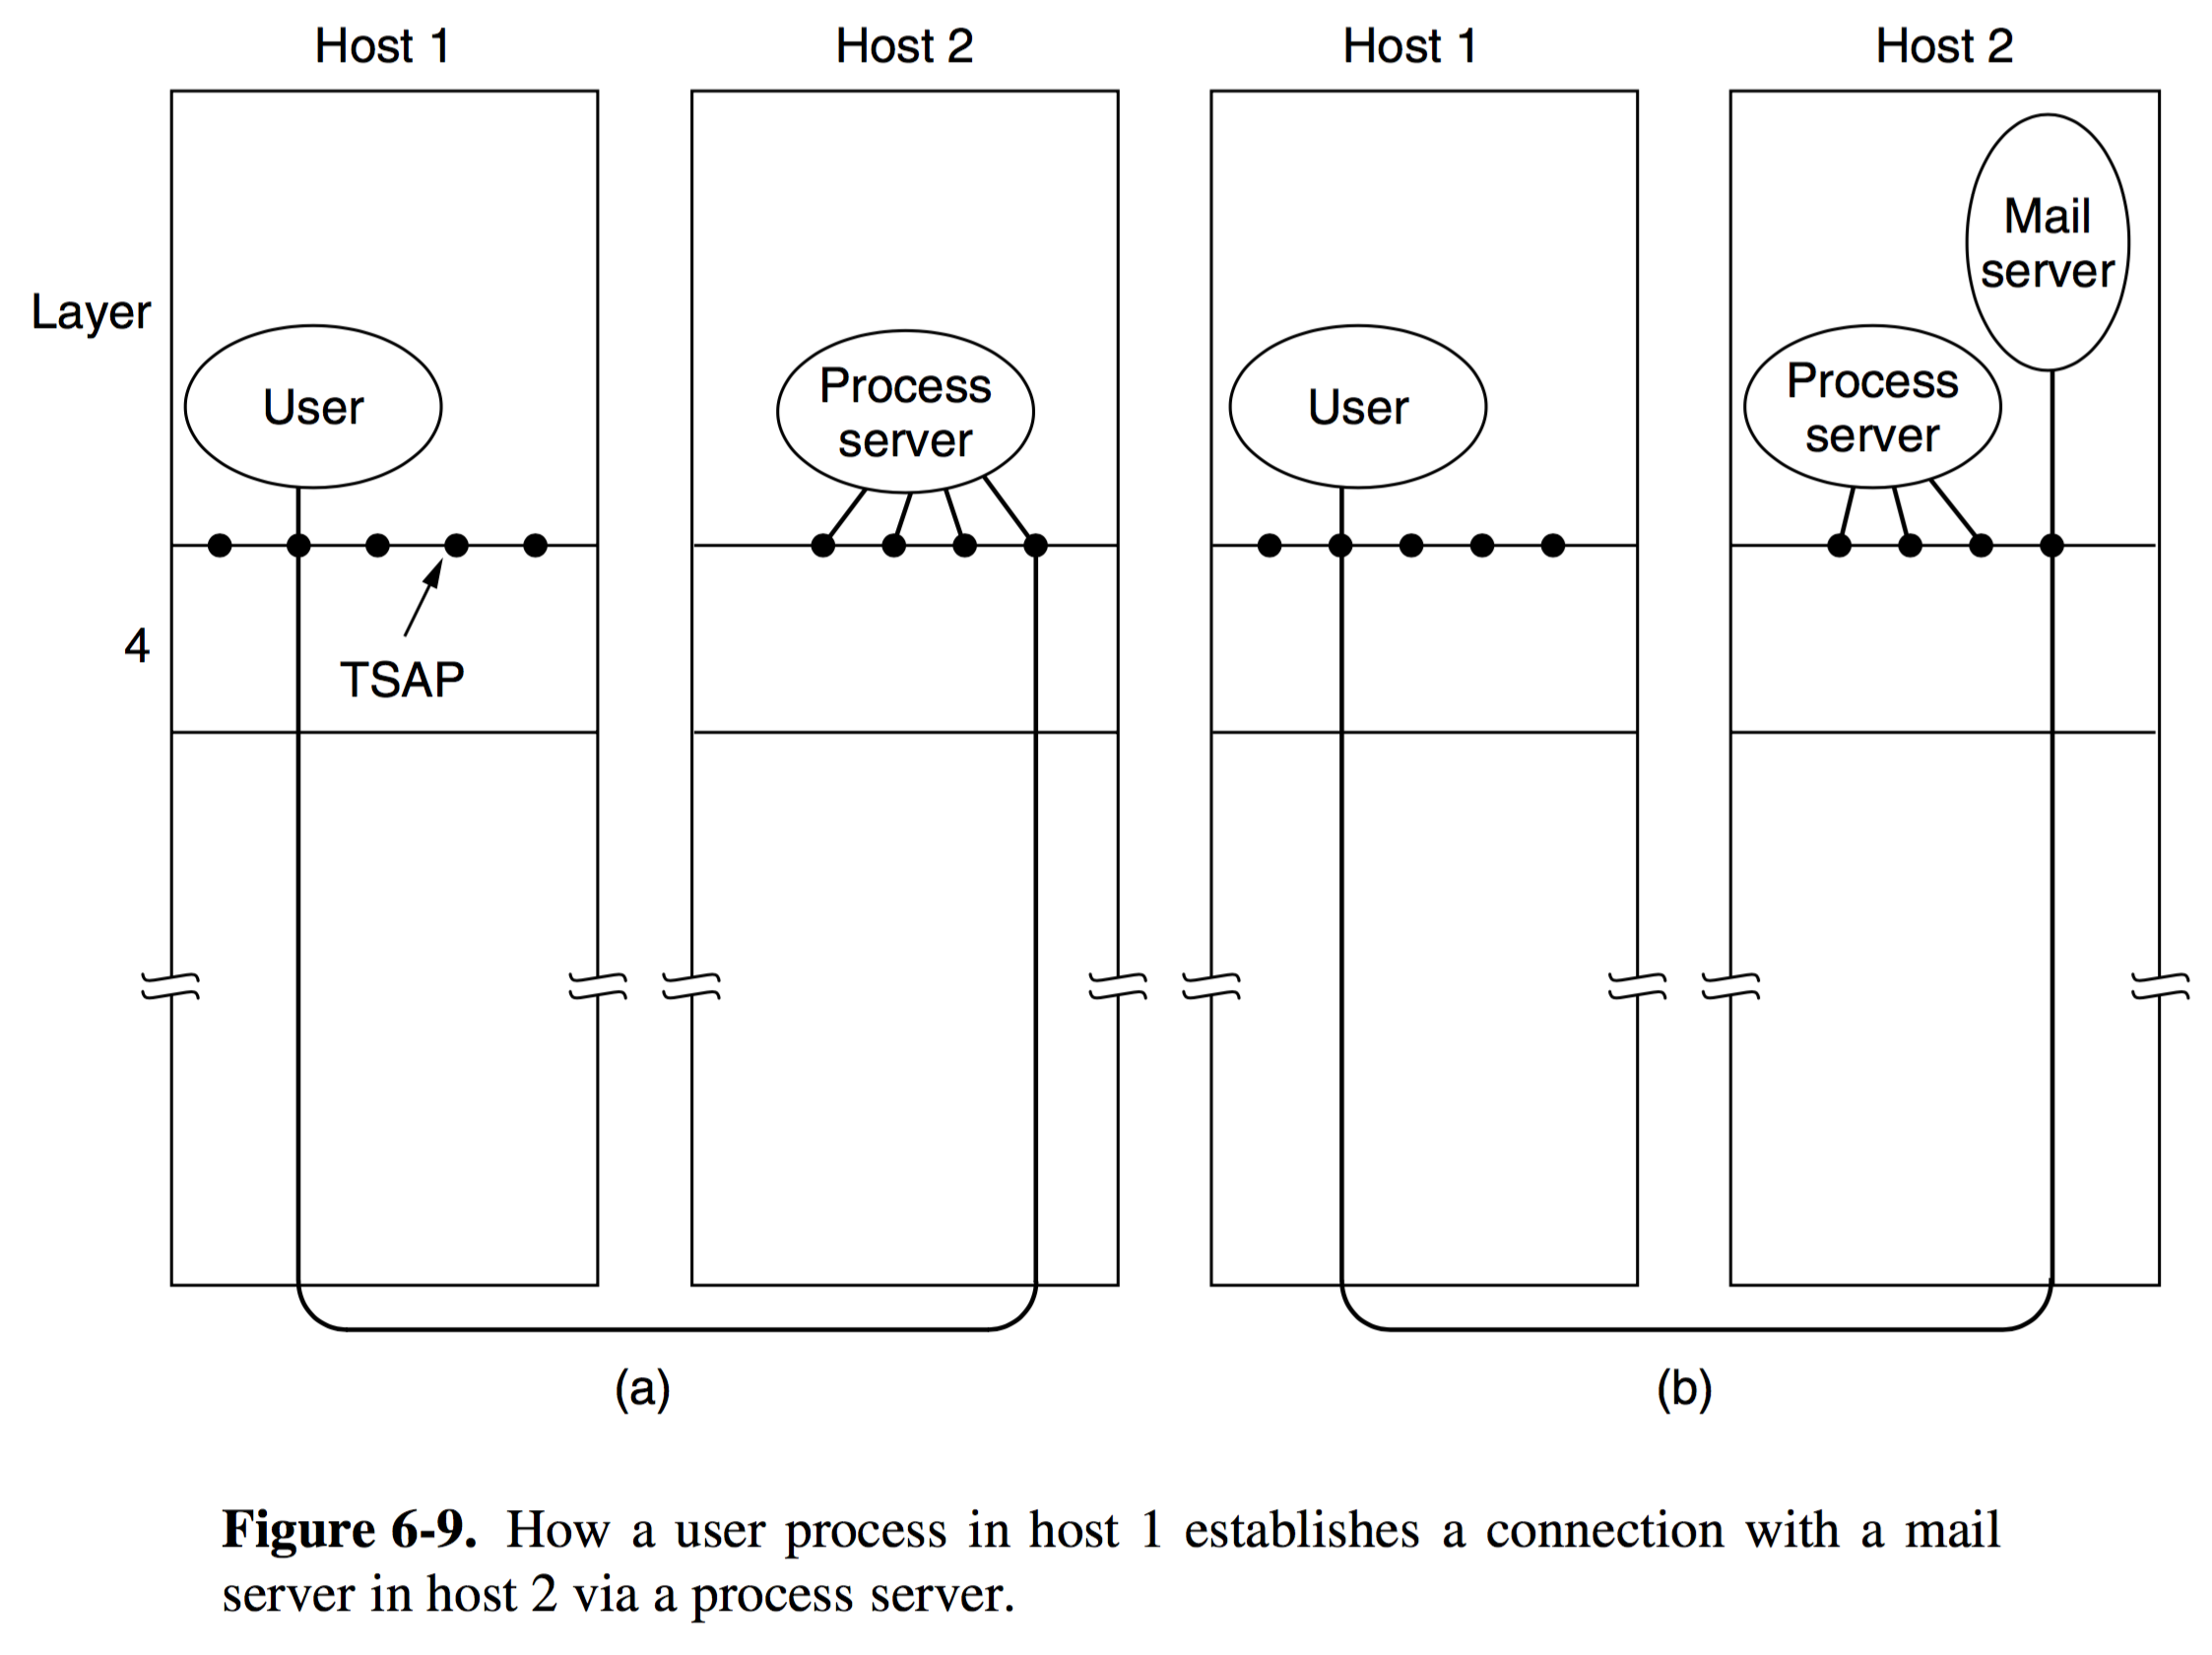
\includegraphics[width=9cm, height=6cm]{./imagenes/conexioninicial.png} 
	\end{center}

	\item  \underline{Solución 3:} Existe un proceso especial llamado \textbf{servidor 
	de nombres} (también llamado servidor de directorio); para encontrar la dirección 
	TSAP correspondiente a un nombre de servicio dado, el usuario establece una 
	conexión con el servidor de nombres (que escucha en un TSAP bien conocido). 
	Entonces el 	usuario envía un mensaje especificando el nombre del servicio y el 
	servidor de nombres le devuelve la dirección TSAP, luego el usuario libera la 
	conexión con el servidor de nombres y establece una nueva con el servicio deseado. 
	Al crearse un servicio nuevo debe registrarse en el servidor de nombres, dando su 
	nombre de servicio como la dirección de su TSAP. El servidor de nombres registra 
	esta 	información en su base de datos.
\end{itemize} 

\subsection{Establecimiento de una conexión}

	\par A primera vista parecería suficiente con que una entidad de transporte enviara tan 
sólo un segmento CONNECTION REQUEST al destino y esperara una respuesta CONNECTION ACCEPTED. El problema ocurre cuando la red puede perder, retrasar, corromper y duplicar paquetes. Este comportamiento causa complicaciones serias.

	\par Imaginemos una subred de datagramas muy congestionada en la que las confirmaciones de recepción casi nunca regresan a tiempo, cada paquete expira y se retransmite algunas veces siguiendo rutas distintas. Algunos paquetes podrían atorarse en un congestionamiento de tráfico de la subred y tardar mucho tiempo en llegar.

	\par La peor pesadilla posible es la siguiente. Un usuario establece una conexión con un banco, envía mensajes indicando al banco que transfiera dinero a la cuenta de una persona y a continuación libera la conexión. Por mala fortuna cada paquete de la transacción se duplica y se almacena en la subred. Tras liberar la conexión todos los paquetes salen de la subred y llegan a destino en orden, solicitando al banco que abra una conexión nueva, transfiera dinero (nuevamente) y libere la conexión.

	\par El banco no tiene manera de saber que son duplicados; debe suponer que esta es una segunda transacción independiente, y transfiere nuevamente el dinero. Estudiaremos el problema de los duplicados retrasados estudiando algoritmos para establecer conexión de una manera confiable, de modo que situaciones como la anterior no puedan ocurrir.

	\par El problema se puede atacar de varias maneras, ninguna de las cuales es muy satisfactoria. Una es usar direcciones de \textbf{transporte desechables}. En este enfoque, cada vez que se requiere una dirección de transporte, se genera una nueva. Cuando una conexión es liberada, se descarta la dirección y no se vuelve a utilizar. Esta estrategia dificulta la conexión con un proceso.

	\par Otra posibilidad es dar a cada conexión un identificador único (es decir, un número de secuencia que se incremente con cada conexión establecida) elegido por la parte iniciadora y puesto en cada segmento, incluyendo el que solicita la conexión. Después de liberar cada conexión, cada entidad de transporte puede actualizar una tabla que liste conexiones obsoletas como pares (entidad de transporte de igual, identificador de conexión). Cada vez que entre una solicitud de conexión, se puede verificar con la tabla para saber si pertenece a una conexión previamente liberada.

	\par Por desgracia, este esquema tiene una falla básica: requiere que cada entidad de transporte mantenga una cierta cantidad de información histórica durante un tiempo indefinido. Esta historia debe persistir tanto en la máquina de origen como en la de destino. De lo contrario, si una máquina falla y pierde su memoria, ya no sabrá qué identificadores de conexión ya han utilizado sus iguales.

	\par Debemos idear un mecanismo para eliminar a los paquetes viejos que aún andan vagando por ahí. Con esta restricción, el problema se vuelve algo más manejable.
El tiempo de vida de un paquete puede restringirse a un máximo conocido mediante el uso de una (o más) de las siguientes técnicas:

	\begin{enumerate}
		\item \textbf{Un diseño de red restringido:} se usa para evitar que los paquetes hagan ciclos, combinado con una manera de limitar el retardo por congestionamiento a través de la trayectoria más larga posible (ahora conocida).
		\item \textbf{Colocar un contador de saltos en cada paquete:} se inicializa el contador de saltos con un valor apropiado y se lo decrementa cada vez que se reenvía el paquete. El protocolo de red descarta cualquier paquete cuyo contador de saltos llega a cero.
		\item \textbf{Marcar el tiempo en cada paquete:} cada paquete lleva la hora en la que fue creado y los enrutadores se ponen de acuerdo en descartar cualquier paquete que haya rebasado cierto tiempo predeterminado. Se requiere que los relojes de los enrutadores estén sincronizados lo que no es una tarea fácil, a menos que se logre la sincronización externamente a la red.
	\end{enumerate}

	\par Pero no solo los paquetes viejos deben eliminarse sino también sus ACK, ya que un ack viejo puede ser el causante de duplicados retrasados.

	\par Introduciremos \textit{T}, que es un múltiplo pequeño del tiempo de vida de paquete máximo verdadero. El múltiplo depende del protocolo y tiene el efecto de hacer más grande a \textit{T}. Si esperamos un tiempo \textit{T} tras el envío de un paquete, podemos estar seguros que todos los rastros suyos ya han desaparecido, y que ni el ni sus ack aparecerán repentinamente de la nada para complicar el asunto. Al limitar los tiempos de vida de los paquetes, es posible proponer una manera a prueba de errores de establecer conexiones seguras.

	\subsubsection{Método de Tomlinson}

		\par La base del método es que el origen etiquete los segmentos con números de secuencia que no se vayan a reutilizar durante \textit{T} segundos. El periodo \textit{T} y la tasa de paquetes por segundo determinan el tamaño de los números de secuencia. De esta manera, sólo un paquete con un número de secuencia específico puede estar pendiente en cualquier momento dado. Aún puede haber duplicados de este paquete, en cuyo caso el destino debe descartarlos.

		\par Sabiendo el tiempo de vida del paquete, el número de secuencia esperado y los números de secuencia de segmentos a confirmar se puede saber si un segmento que llega es duplicado o no. Si el paquete no expiró y su número de secuencia es menor que el número de secuencia esperado, entonces ya se lo recibió y confirmó, en cambio si su número de secuencia es el número de secuencia de uno de los segmentos a confirmar, entonces es duplicado.

		\par Para resolver el problema de una máquina que pierde toda la memoria acerca de su estado tras de una caída, Tomlinson propuso equipar cada host con un reloj. Los relojes de los distintos hosts no necesitan estar sincronizados. Se supone que cada reloj tiene la forma de un contador binario que se incrementa a sí mismo a intervalos uniformes. Además, la cantidad de bits del contador debe ser igual o mayor que la cantidad de bits en los números de secuencia. Por último, y lo más importante, se supone que el reloj continúa operando aunque el host falle.

		\par Cuando se establece una conexión, los \textit{k} bits de menor orden del reloj se usan como número de secuencia inicial de \textit{k} bits. Cada conexión comienza a numerar sus segmentos con un número de secuencia inicial diferente. El espacio de secuencia también debe ser lo bastante grande para que cuando los números de secuencia se reinicien, los segmentos antiguos con el mismo número de secuencia hayan desaparecido hace mucho tiempo. En la figura 6-10(a) se muestra esta relación lineal entre tiempo y números secuenciales iniciales.

		\begin{center} 
			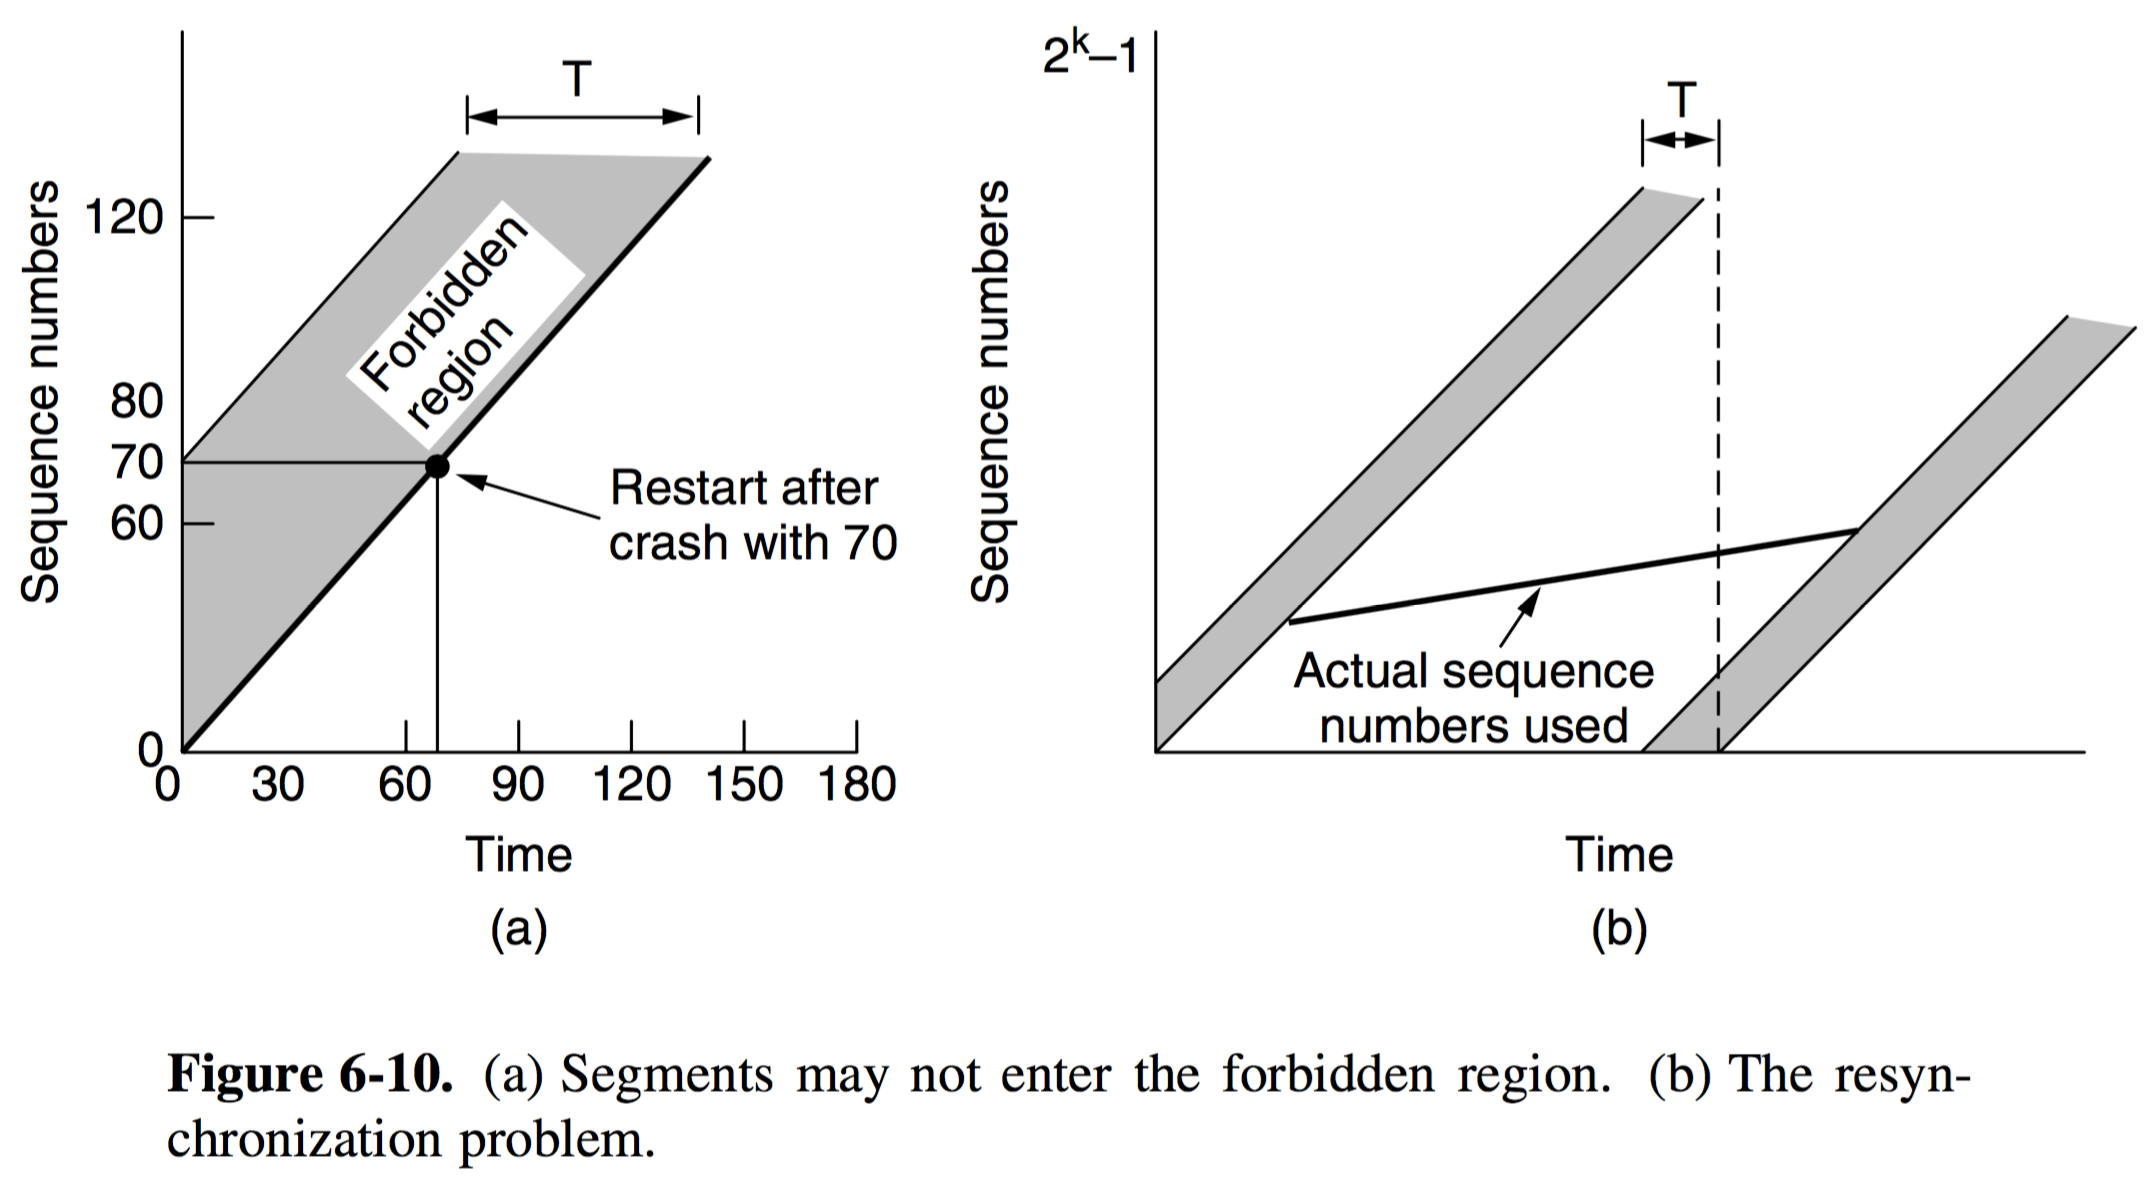
\includegraphics[width=9cm, height=6cm]{./imagenes/tomlinson.png} 
		\end{center}

		\par Una vez que ambas entidades de transporte han acordado un número de secuencia inicial, puede usarse cualquier protocolo para el control de flujo de datos. La curva inicial de números de secuencia (indicada por la línea gruesa de la figura anterior) no es realmente lineal, sino una escalera, ya que el reloj avanza en pasos discretos. Por sencillez ignoramos este detalle.

		\par Para mantener los números de secuencia fuera de la región prohibida, necesitamos tener cuidado con dos aspectos. Si un host envía muchos datos con demasiada rapidez en una conexión recién abierta, el número de secuencia actual contra la curva de tiempo puede subir en forma más pronunciada que el número de secuencia inicial contra la curva de tiempo, lo cual provoca que el número de secuencia entre a la región prohibida. Para evitar que esto ocurra, la tasa máxima de datos en cualquier conexión es de un segmento por cada pulso de reloj. La entidad de transporte debe esperar hasta que el reloj emita un pulso antes de abrir una nueva conexión después de un reinicio por falla, no sea que el mismo número se utilice dos veces.
Ambos puntos son argumentos a favor de un pulso de reloj corto (unos cuantos milisegundos). Esto es suponiendo que la relación tiempo a número de secuencia inicial es la función identidad. La idea es mantener los números de segmento generados por debajo de la línea gruesa correspondiente a esa relación.

		\par Entrar a la región prohibida por la parte inferior al enviar con demasiada rapidez no es la única forma de meterse en problemas. De la figura 6-10(b) podemos ver que, a cualquier tasa de datos menor que la tasa de reloj, la curva de números de secuencia actuales utilizados vs el tiempo entrará en un momento dado a la región prohibida desde la izquierda, mientras los números de secuencia se reinician. Entre mayor sea la pendiente de los números de secuencia actuales, más se retardará este evento. Justo antes de enviar cada segmento, la entidad de transporte debe comprobar que no esté a punto de entrar en la región prohibida; de ser así debe retardar el segmento durante \textit{T} segundos o resincronizar los números de secuencia.

		\par El método basado en reloj resuelve el problema de no poder diferenciar los segmentos duplicados con retardo de los segmentos nuevos. Sin embargo, hay un inconveniente práctico en cuanto a su uso para establecer conexiones. Como por lo general no recordamos los números de secuencia de una conexión a otra en el destino, aún no tenemos forma de saber si un segmento CONNECTION REQUEST que contiene un número de secuencia inicial es un duplicado de una conexión reciente.

		\par Para resolver este problema específico, Tomlinson (1975) desarrolló el \textbf{acuerdo de tres vías} (\textit{threeway handshake}). Este protocolo de establecimiento implica que un igual verifique con el otro que la solicitud de conexión sea realmente actual. El procedimiento normal de establecimiento al iniciar el \textit{host 1} se muestra en la figura siguiente figura, en su inciso (a). El \textit{host 1} escoge un número de secuencia, \textit{x}, y envía al \textit{host 2} un segmento CONNECTION REQUEST que contiene ese número. El \textit{host 2} responde con un segmento ACK para confirmar la recepción de \textit{x} y anunciar su propio número de secuencia inicial, \textit{y}. Por último, el \textit{host 1} confirma la recepción del número de secuencia inicial seleccionado por el \textit{host 2} en el primer segmento de datos que envía.

		\begin{center} 
			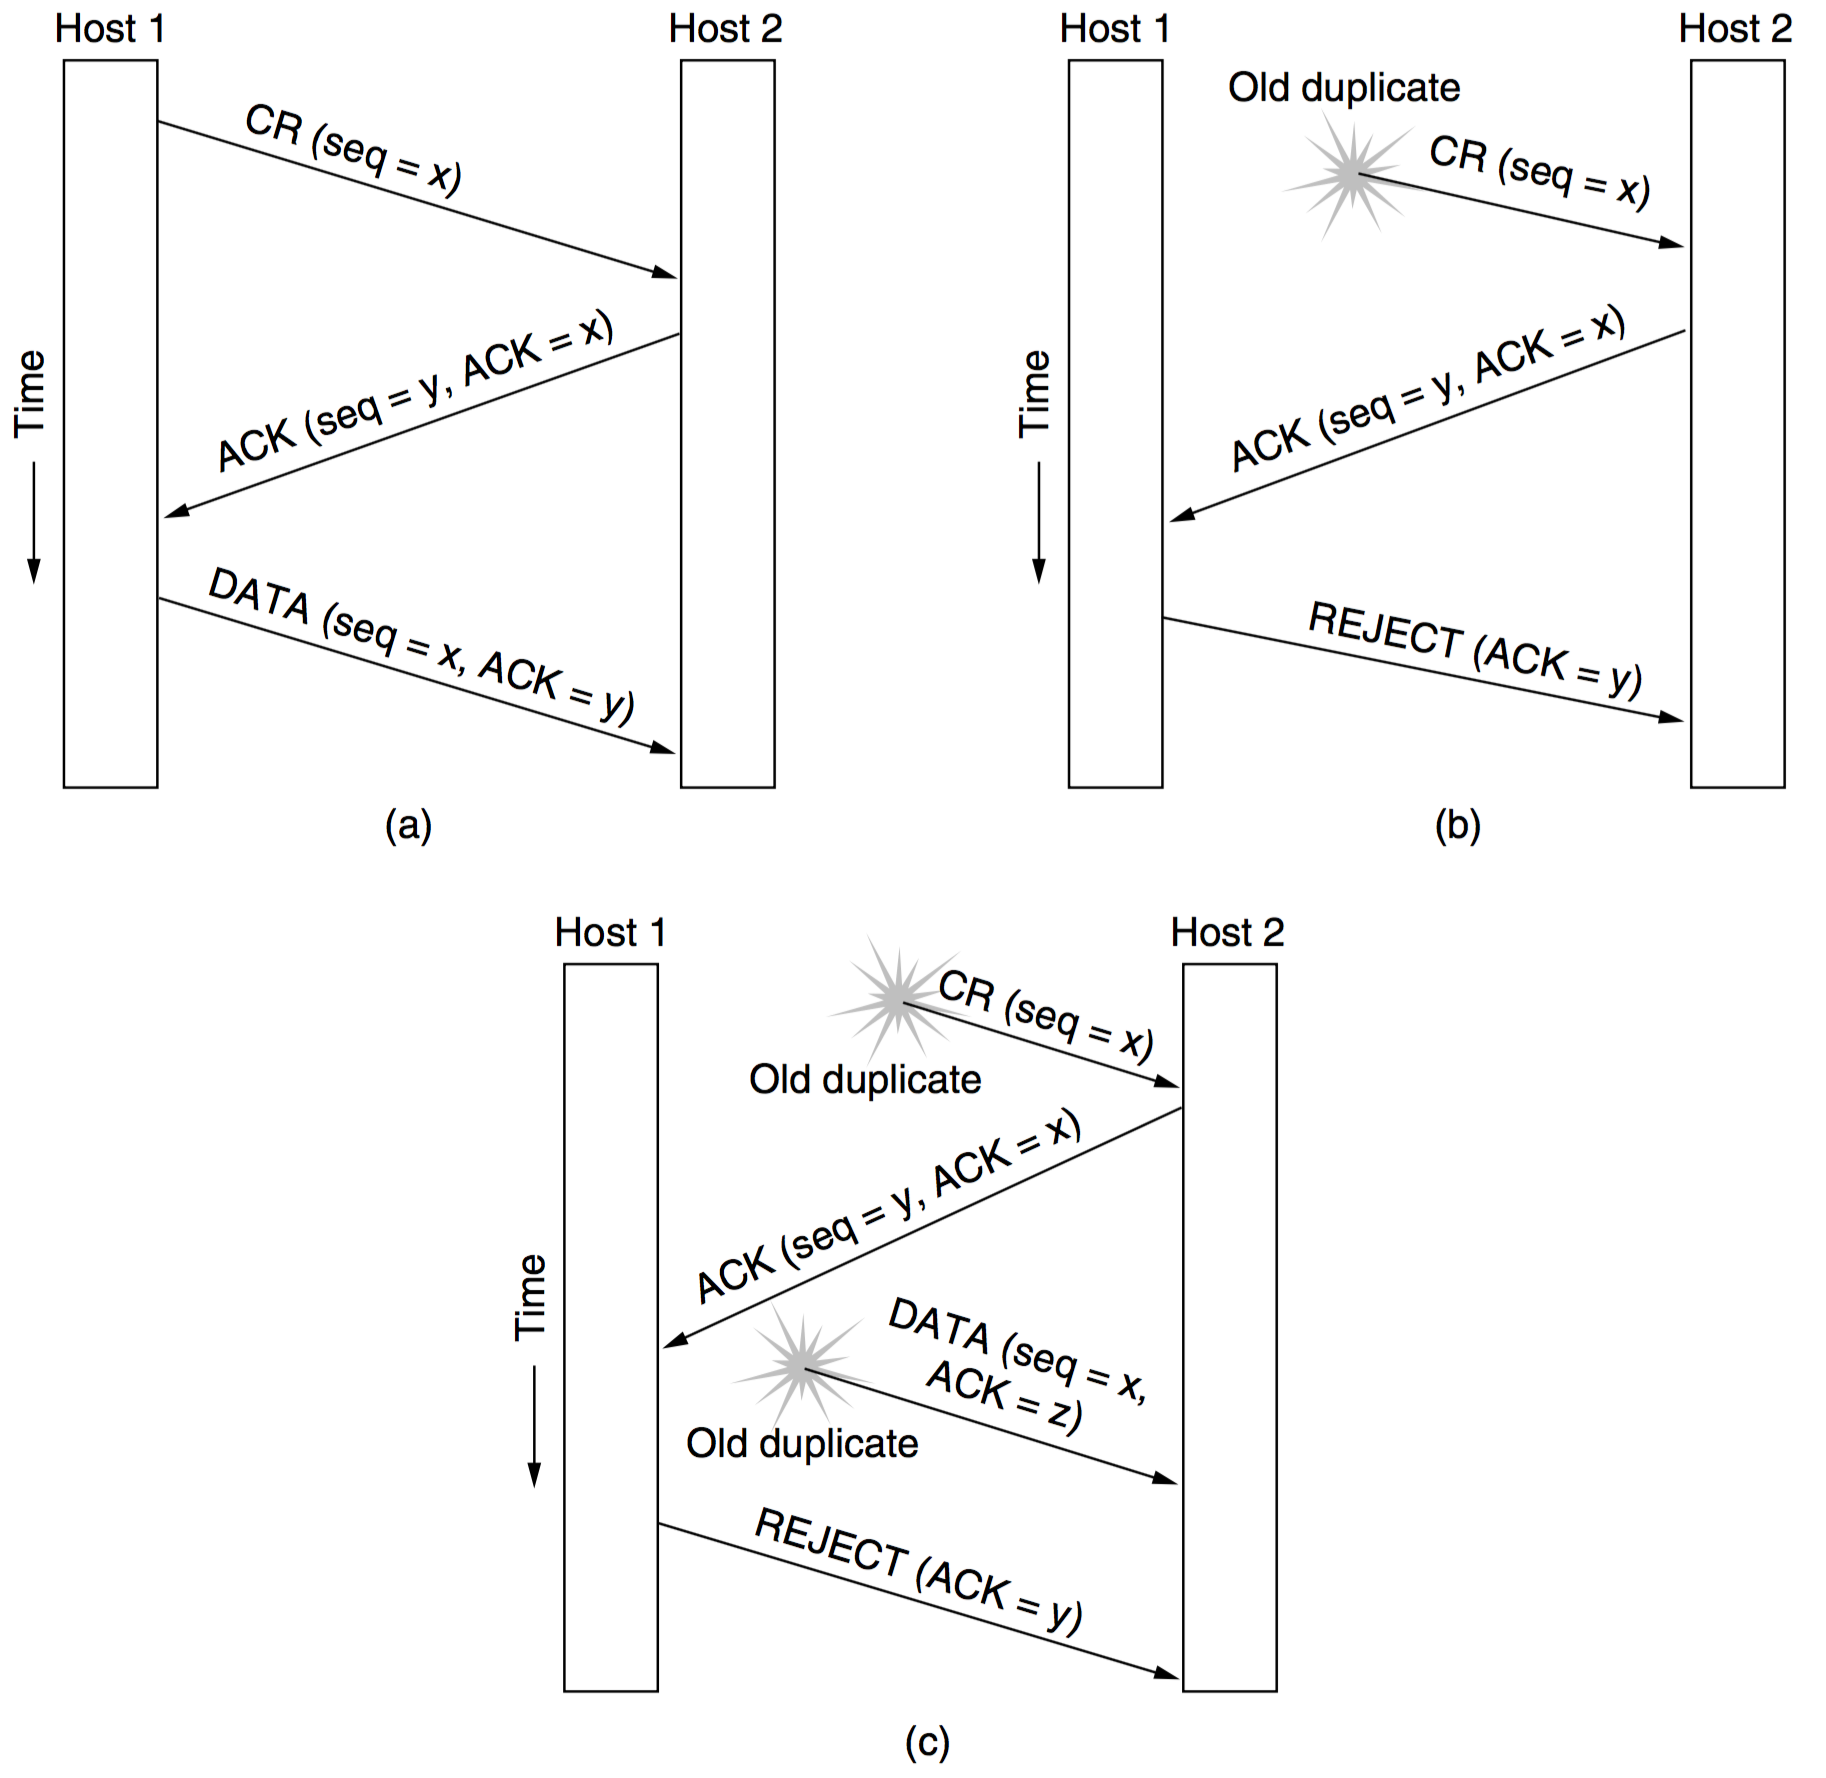
\includegraphics[width=8cm, height=6cm]{./imagenes/tomlinson2.png} 
		\end{center}

		\par En la parte (b) de la figura, el primer segmento es un CONNECTION REQUEST duplicado con retardo de una conexión antigua. Este segmento llega al \textit{host 2} sin el conocimiento del \textit{host 1}. El \textit{host 2} reacciona a este segmento y envía al \textit{host 1} un segmento ACK, para solicitar en efecto la comprobación de que el \textit{host 1} haya tratado realmente de establecer una nueva conexión. Cuando el \textit{host 1} rechaza el intento del \textit{host 2} por establecer una conexión, el \textit{host 2} se da cuenta de que fue engañado por un duplicado con retardo y abandona la conexión. De esta manera, un duplicado con retardo no causa daño.

		\par El peor caso ocurre cuando en la subred deambulan tanto un segmento CONNECTION REQUEST con retardo como un ACK. Este caso se muestra en el inciso (c) de la figura. Como en el ejemplo anterior, el \textit{host 2} recibe un CONNECTION REQUEST con retardo y lo contesta. En este momento es imprescindible tener en cuenta que el \textit{host 2} ha propuesto usar y como número de secuencia inicial para el tráfico del \textit{host 2} al \textit{host 1}, sabiendo bien que no existen todavía segmentos que contengan el número de secuencia y ni confirmaciones de recepción de y. Cuando llega el segundo segmento con retardo al \textit{host 2}, el hecho de que se confirmó la recepción de z en lugar de y indica al \textit{host 2} que éste también es un duplicado antiguo. Lo importante que debemos tener en cuenta aquí es que no hay una combinación de segmentos antiguos que puedan provocar la falla del protocolo y permitan establecer una conexión accidental cuando nadie la quiere.

\subsection{Liberación de una conexión}

	\par Cuando ya no se necesita una conexión, debe liberarse para desocupar espacio en las tablas de las dos entidades de transporte. Hay dos estilos para terminar una conexión: \textbf{liberación asimétrica} y \textbf{liberación simétrica}. La liberación asimétrica es la manera en que funciona el sistema telefónico: cuando una de las partes cuelga, se interrumpe la conexión. La liberación simétrica trata la conexión como dos conexiones unidireccionales distintas y requiere que cada una se libere por separado.

	\par La liberación asimétrica es abrupta y puede provocar la pérdida de datos. Considere el escenario de la figura siguiente.
	
	\begin{center}
		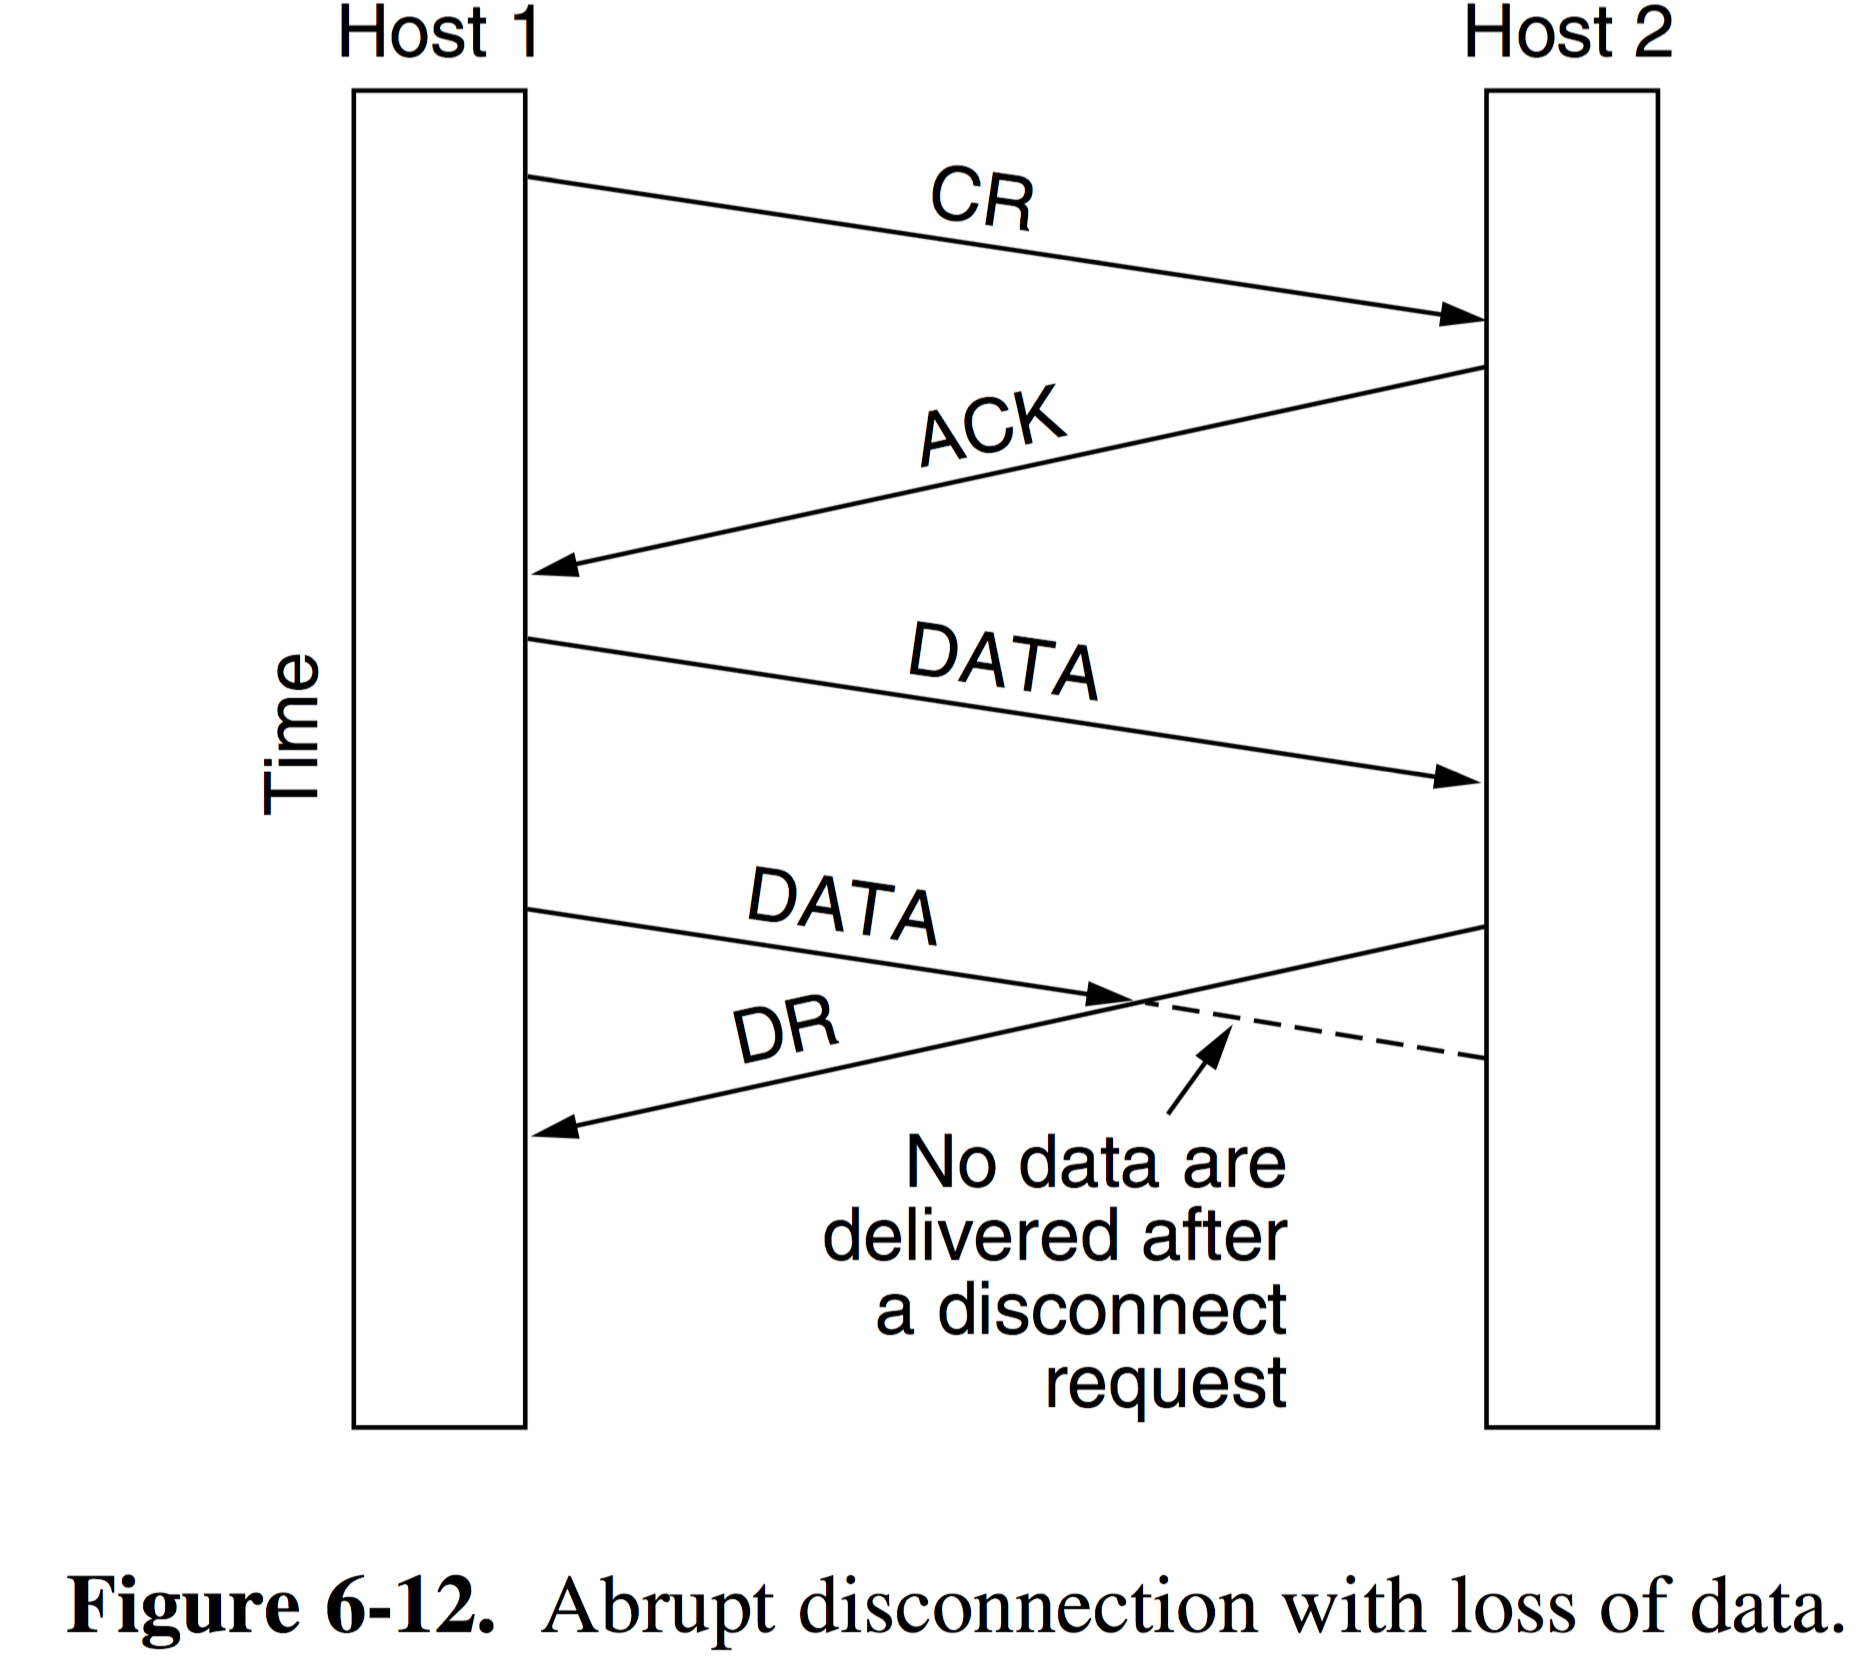
\includegraphics[width=7cm, height=5cm]{./imagenes/liberacion.png}
	\end{center}
	
	\par Una vez que se establece la conexión, el \textit{host 1} envía un segmento que llega en forma apropiada al \textit{host 2}. A continuación, el \textit{host 1} envía otro segmento. Por desgracia, el \textit{host 2} emite un DISCONNECT antes de que llegue el segundo segmento. El resultado es que se libera la conexión y se pierden los datos.

	\par Se requiere un protocolo de liberación más sofisticado para evitar la pérdida de los datos. Una posibilidad es usar la liberación simétrica, en la que cada dirección se libera en forma independiente de la otra. Aquí, un host puede continuar recibiendo datos, aun después de haber enviado un segmento DISCONNECT.

	\par La liberación simétrica es ideal cuando cada proceso tiene una cantidad fija de datos por enviar y sabe con certeza cuándo los ha enviado. En otras situaciones, el proceso de determinar si se ha efectuado o no todo el trabajo y si debe terminar o no la conexión no es tan obvio. Podríamos pensar en un protocolo en el que el \textit{host 1} diga: “Ya terminé. ¿Terminaste también?” Si el \textit{host 2} responde: “Ya terminé también. Adiós”, la conexión se puede liberar sin problemas.

	\par Por desgracia, este protocolo no siempre funciona. Hay un problema famoso que tiene que ver con ese asunto. Se conoce como el \textbf{problema de los dos ejércitos}.

\subsubsection{Problema de los dos ejércitos}

	\begin{center}
		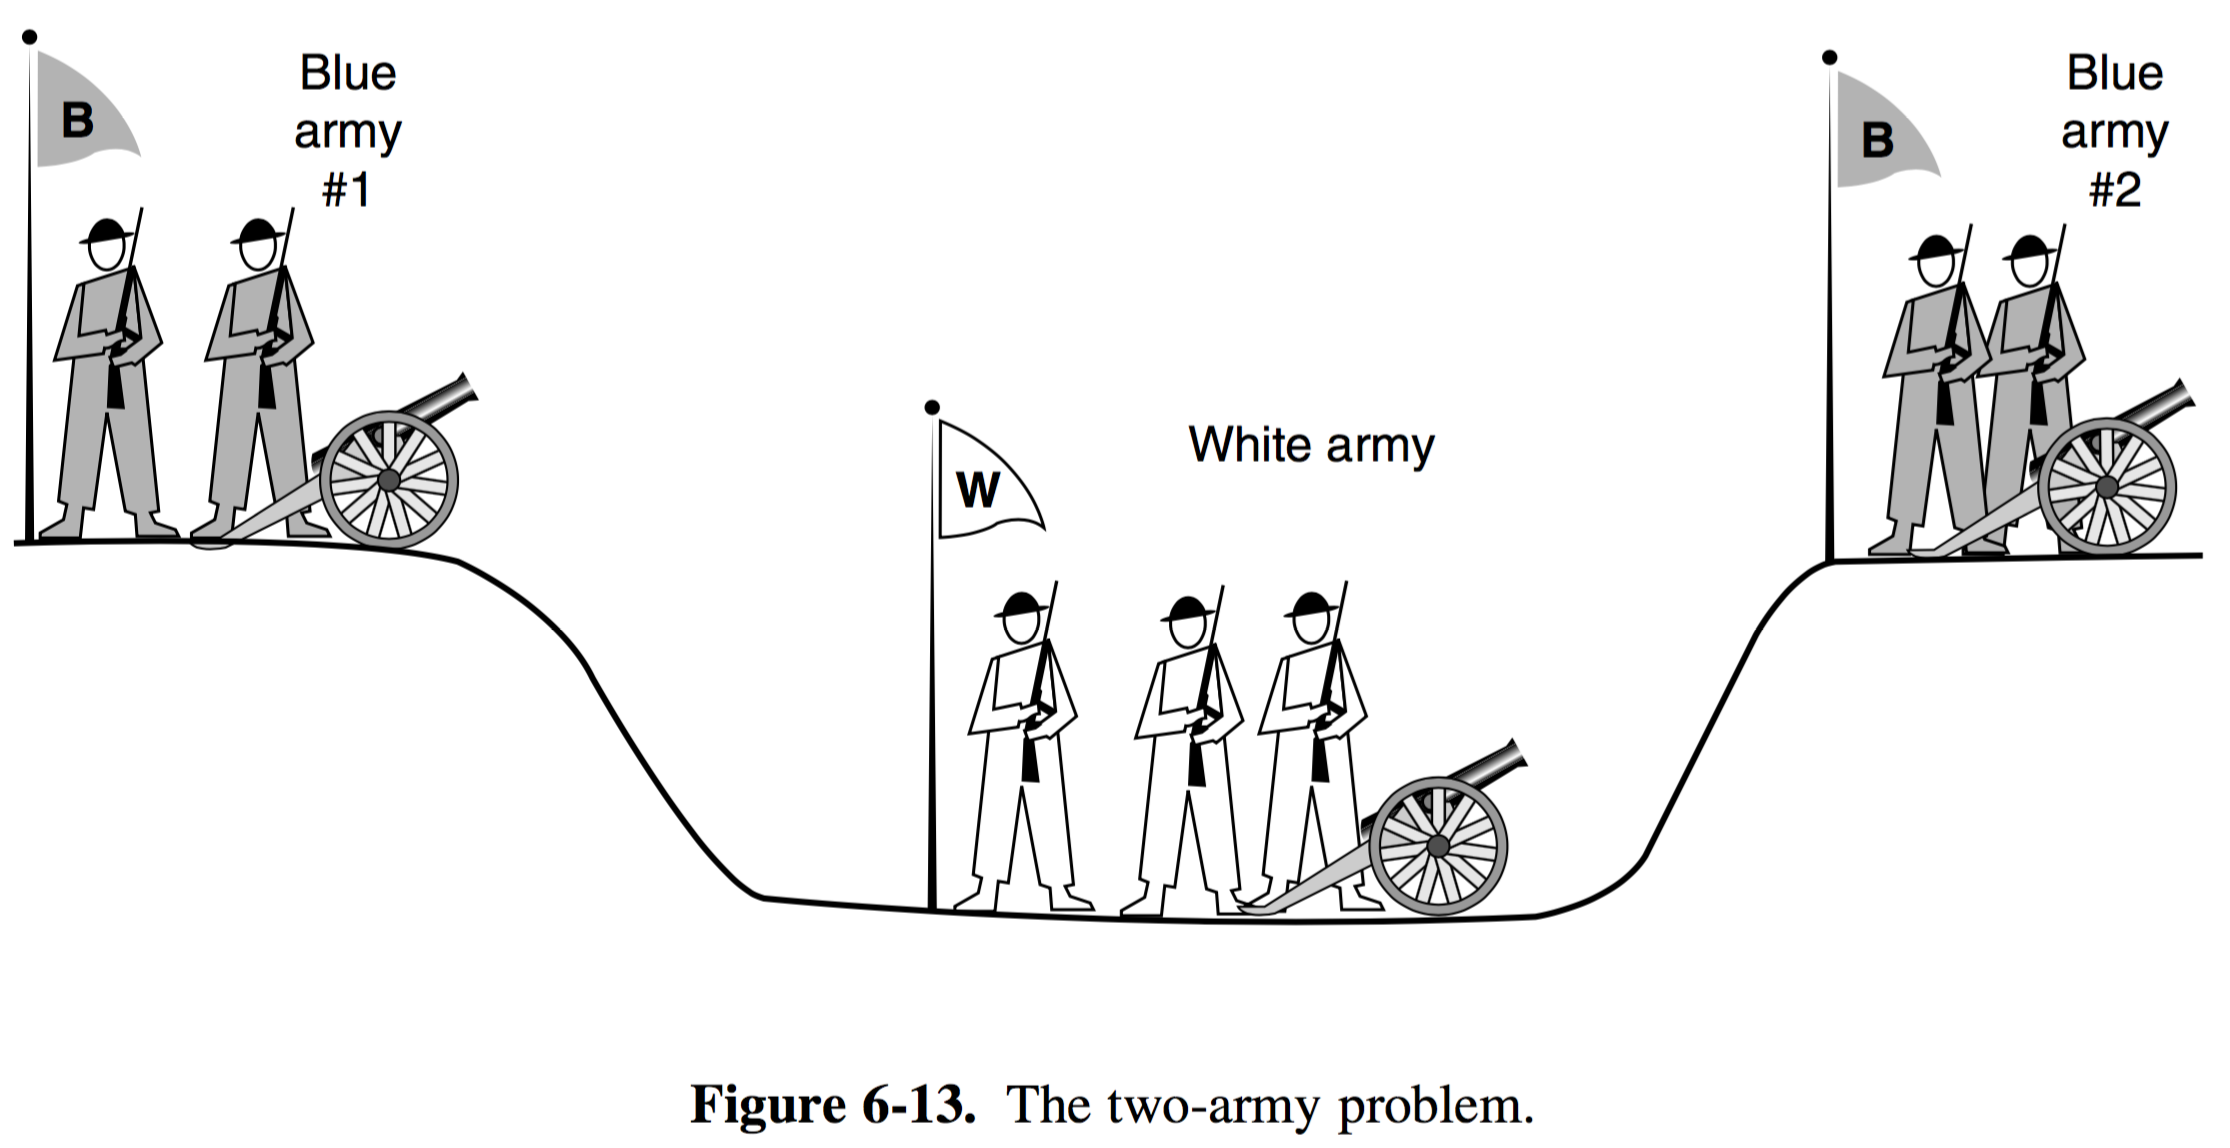
\includegraphics[width=9cm, height=6cm]{./imagenes/ejercitos.png}
	\end{center}

	\par Imagine que un ejército blanco está acampado en un valle, como se muestra en la figura 6-13. En los dos cerros que rodean al valle hay ejércitos azules. El ejército blanco es más grande que cualquiera de los dos ejércitos azules por separado, pero juntos éstos son más grandes que el ejército blanco. Si cualquiera de los dos ejércitos azules ataca por su cuenta, será derrotado, pero si los dos atacan a la vez obtendrán la victoria.

	\par Los ejércitos azules quieren sincronizar sus ataques. Sin embargo, su único medio de comunicación es el envío de mensajeros a pie a través del valle, donde podrían ser capturados y se perdería el mensaje (es decir, tienen que usar un canal de comunicación no confiable). La pregunta es: ¿Existe un protocolo que permita que los ejércitos azules ganen?
	
	\par Supongamos que el comandante del \textit{ejército azul \#1} envía un mensaje que dice: “Propongo que ataquemos en el horario H. ¿Qué les parece?” Ahora supongamos que llega el mensaje y que el comandante del \textit{ejército azul \#2} está de acuerdo, y que su respuesta llega con seguridad al \textit{ejército azul \#1}. ¿Ocurrirá el ataque? Es probable que no, porque el comandante \#2 no sabe si su respuesta llegó. Si no llegó, el \textit{ejército azul \#1} no atacará, y sería tonto de su parte emprender el combate.
	
	\par Mejoremos ahora el protocolo para convertirlo en un \textbf{acuerdo de tres vías}. El iniciador de la propuesta original debe confirmar la recepción de la respuesta. Suponiendo que no se pierden mensajes, el \textit{ejército azul \#2} recibirá la confirmación de recepción, pero ahora el que dudará será el comandante del \textit{ejército azul \#1}. A fin de cuentas, no sabe si ha llegado su confirmación de recepción y, si no llegó, sabe que el \textit{ejército \#2} no atacará. Podríamos probar ahora un protocolo de acuerdo de cuatro vías, pero tampoco ayudaría.
	
	\par Podemos demostrar que no existe un protocolo que funcione. Supongamos que existiera algún protocolo. El último mensaje del protocolo es esencial, o no lo es. Si no lo es, podemos eliminarlo (así como los demás mensajes no esenciales) hasta que quede un protocolo en el que todos los mensajes sean esenciales. ¿Qué ocurre si el mensaje final no pasa? Acabamos de decir que es esencial, por lo que, si se pierde, el ataque no ocurrirá. Dado que el emisor del mensaje final nunca puede estar seguro de su llegada, no se arriesgará a atacar. Peor aún, el otro ejército azul sabe esto, por lo que tampoco atacará.

	\par Para ver la relevancia del problema de los dos ejércitos en relación con la liberación de conexiones, simplemente sustituya “atacar” por “desconectar”. Si ninguna de las partes está preparada para desconectarse hasta estar convencida de que la otra está preparada para desconectarse también, nunca ocurrirá la desconexión.
	
	\par Vamos a permitir que cada parte decida cuando la conexión está terminada. Este es un problema más sencillo. En la figura 6-14 se muestran cuatro escenarios de liberación de conexión usando un \textit{acuerdo de 3 vías}. Aunque este protocolo no es infalible, generalmente es adecuado.
	
	\begin{center}
		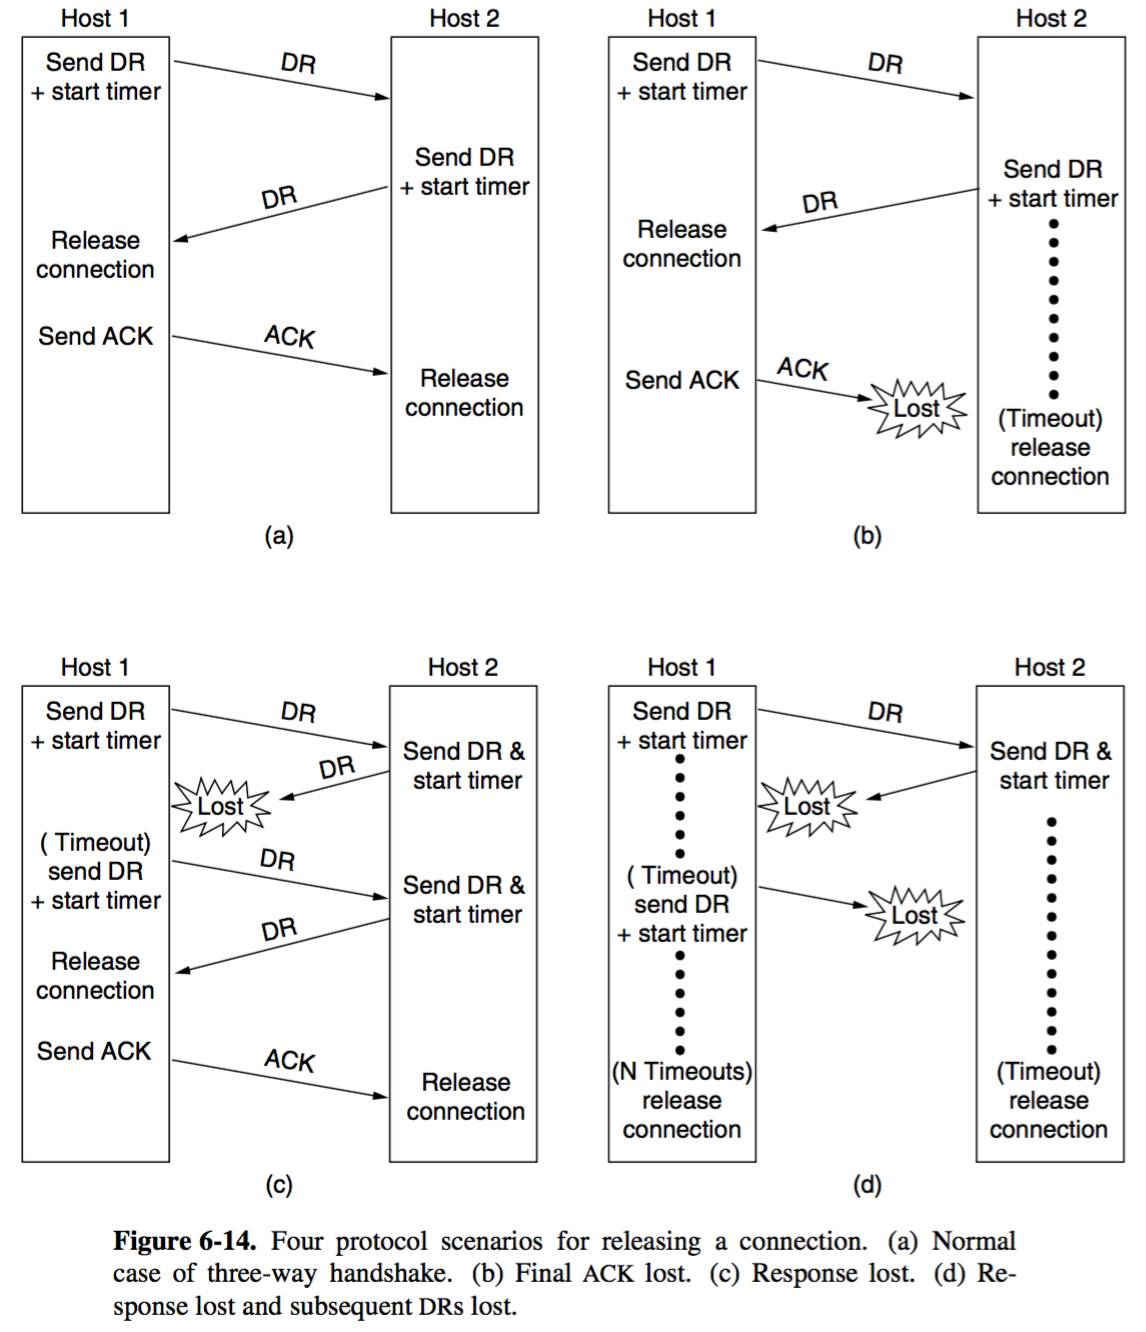
\includegraphics[width=11cm, height=10cm]{./imagenes/conexion.png}
	\end{center}

	\par En la figura 6-14(a) vemos el caso normal en el que uno de los usuarios envía un segmento DR de solicitud de desconexión (DISCONNECTION REQUEST) con el fin de iniciar la liberación de una conexión. Al llegar, el receptor devuelve también un segmento DR e inicia un temporizador, por si acaso se pierde su DR. Cuando este DR llega, el emisor original envía de regreso un segmento ACK y libera la conexión. Finalmente, cuando llega el segmento ACK, el receptor también libera la conexión. Liberar una conexión significa que la entidad de transporte remueve la información sobre la conexión de su tabla de conexiones abiertas y avisa de alguna manera al dueño de la conexión (el usuario de transporte).
	
	\par Si se pierde el último segmento ACK, como se muestra en la figura 6-14(b), el temporizador salva la situación. Al expirar el temporizador, la conexión se libera de todos modos.

	\par Ahora consideremos el caso en el que se pierde el segundo DR. El usuario que inicia la desconexión no recibirá la respuesta esperada, su temporizador expirará y todo comenzará de nuevo. En la figura 6-14(c) vemos la manera en que esto funciona, suponiendo que la segunda vez no se pierden segmentos, y que todos se entregan correctamente y a tiempo.

	\par Nuestro último escenario, la figura 6-14(d), es el mismo que en la figura 6-14(c), excepto que ahora suponemos que todos los intentos repetidos de retransmitir el segmento DR también fallan debido a los segmentos perdidos. Después de N reintentos, el emisor simplemente se da por vencido y libera la conexión. Mientras tanto, expira el temporizador del receptor y también se sale.
	
	\par Aunque por lo general basta con este protocolo, en teoría puede fallar si se pierden el DR inicial y N retransmisiones. El emisor se dará por vencido y liberará la conexión, pero el otro lado no sabrá nada sobre los intentos de desconexión y seguirá plenamente activo. Esta situación provoca una \textbf{conexión semiabierta}.

	\par Pudimos haber evitado este problema al impedir que el emisor se diera por vencido después de N reintentos y obligarlo a seguir insistiendo hasta recibir una respuesta. No obstante, si permitimos que expire el temporizador en el otro lado, entonces el emisor continuará por siempre, pues nunca llegará una respuesta. 

	\par Una manera de eliminar las conexiones semiabiertas es tener una regla que diga que, si no han llegado segmentos durante ciertos segundos, se libera automáticamente la conexión. De esta manera, si un lado llega a desconectarse, el otro lado detectará la falta de actividad y también se desconectará. Esta regla también se encarga del caso donde se rompe la conexión (porque la red ya no puede entregar paquetes entre los hosts) sin que ninguno de los extremos se desconecte. Por supuesto que si se pone en práctica esta regla, es necesario que cada entidad de transporte tenga un temporizador que se detenga y se reinicie cada vez que se envíe un segmento.

	\par No se puede garantizar absolutamente que cuando se libera una conexión no ocurre pérdida de datos, pero si se puede limitar mucho que esto suceda. La nueva solución es muchísimo mejor que la de liberación asimétrica.

\subsection{Control de flujo y almacenamiento en búfer}

\subsubsection{Uso de búferes}

	\par Si la subred provee un servicio de datagramas, la entidad de transporte emisora debe manejar búferes para los mensajes de salida. Si el receptor sabe que el emisor almacena en búfer todas los segmentos hasta que se confirma su recepción, el receptor podría o no dedicar búferes específicos a conexiones específicas según considere necesario. Cuando entra un segmento, el receptor intenta adquirir un búfer nuevo, si hay uno disponible, se acepta el segmento; de otro modo se lo descarta. Dado que el emisor está preparado para retransmitir los segmentos perdidos por la subred, no hay nada de malo en hacer que el receptor se deshaga de los segmentos. El emisor simplemente sigue intentando hasta que recibe una ACK.
	
	\par Aun si el receptor está de acuerdo en usar búferes, todavía queda la cuestión del tamaño de estos. Tres ideas: 
	\begin{enumerate}
		\item \underline{Uso de búferes de tamaño fijo:} si la mayoría de los segmentos tiene aproximadamente el mismo tamaño organizar los búferes como un grupo de búferes de tamaño idéntico, con un segmento por búfer como en la figura 15 a). El problema con este método es que si hay una variación grande en el tamaño de los segmentos, el grupo de búferes de tamaño fijo presenta problemas. Si el tamaño de búfer se escoge igual al tamaño del segmento más grande, se desperdiciará espacio cada vez que llegue un segmento corto. Si el tamaño se escoge menor que el tamaño máximo de segmento, se requerirán varios búferes para los segmentos grandes, con la complejidad inherente.

		\item \underline{Uso de búferes de tamaño variable:} la ventaja aquí es un mejor uso de la memoria, al costo de una administración de búferes más complicada. Esta solución se ve ilustrada en la figura 6-15 b).

		\item \underline{Búfer Circular:}	dedicar un solo búfer circular grande por conexión, como en la figura 6-15 c). Con este método se hace buen uso de la memoria cuando todas las conexiones tienen una carga alta, pero es deficiente si algunas conexiones cuentan con poca carga.
	\end{enumerate}	 
	
	\begin{center}
		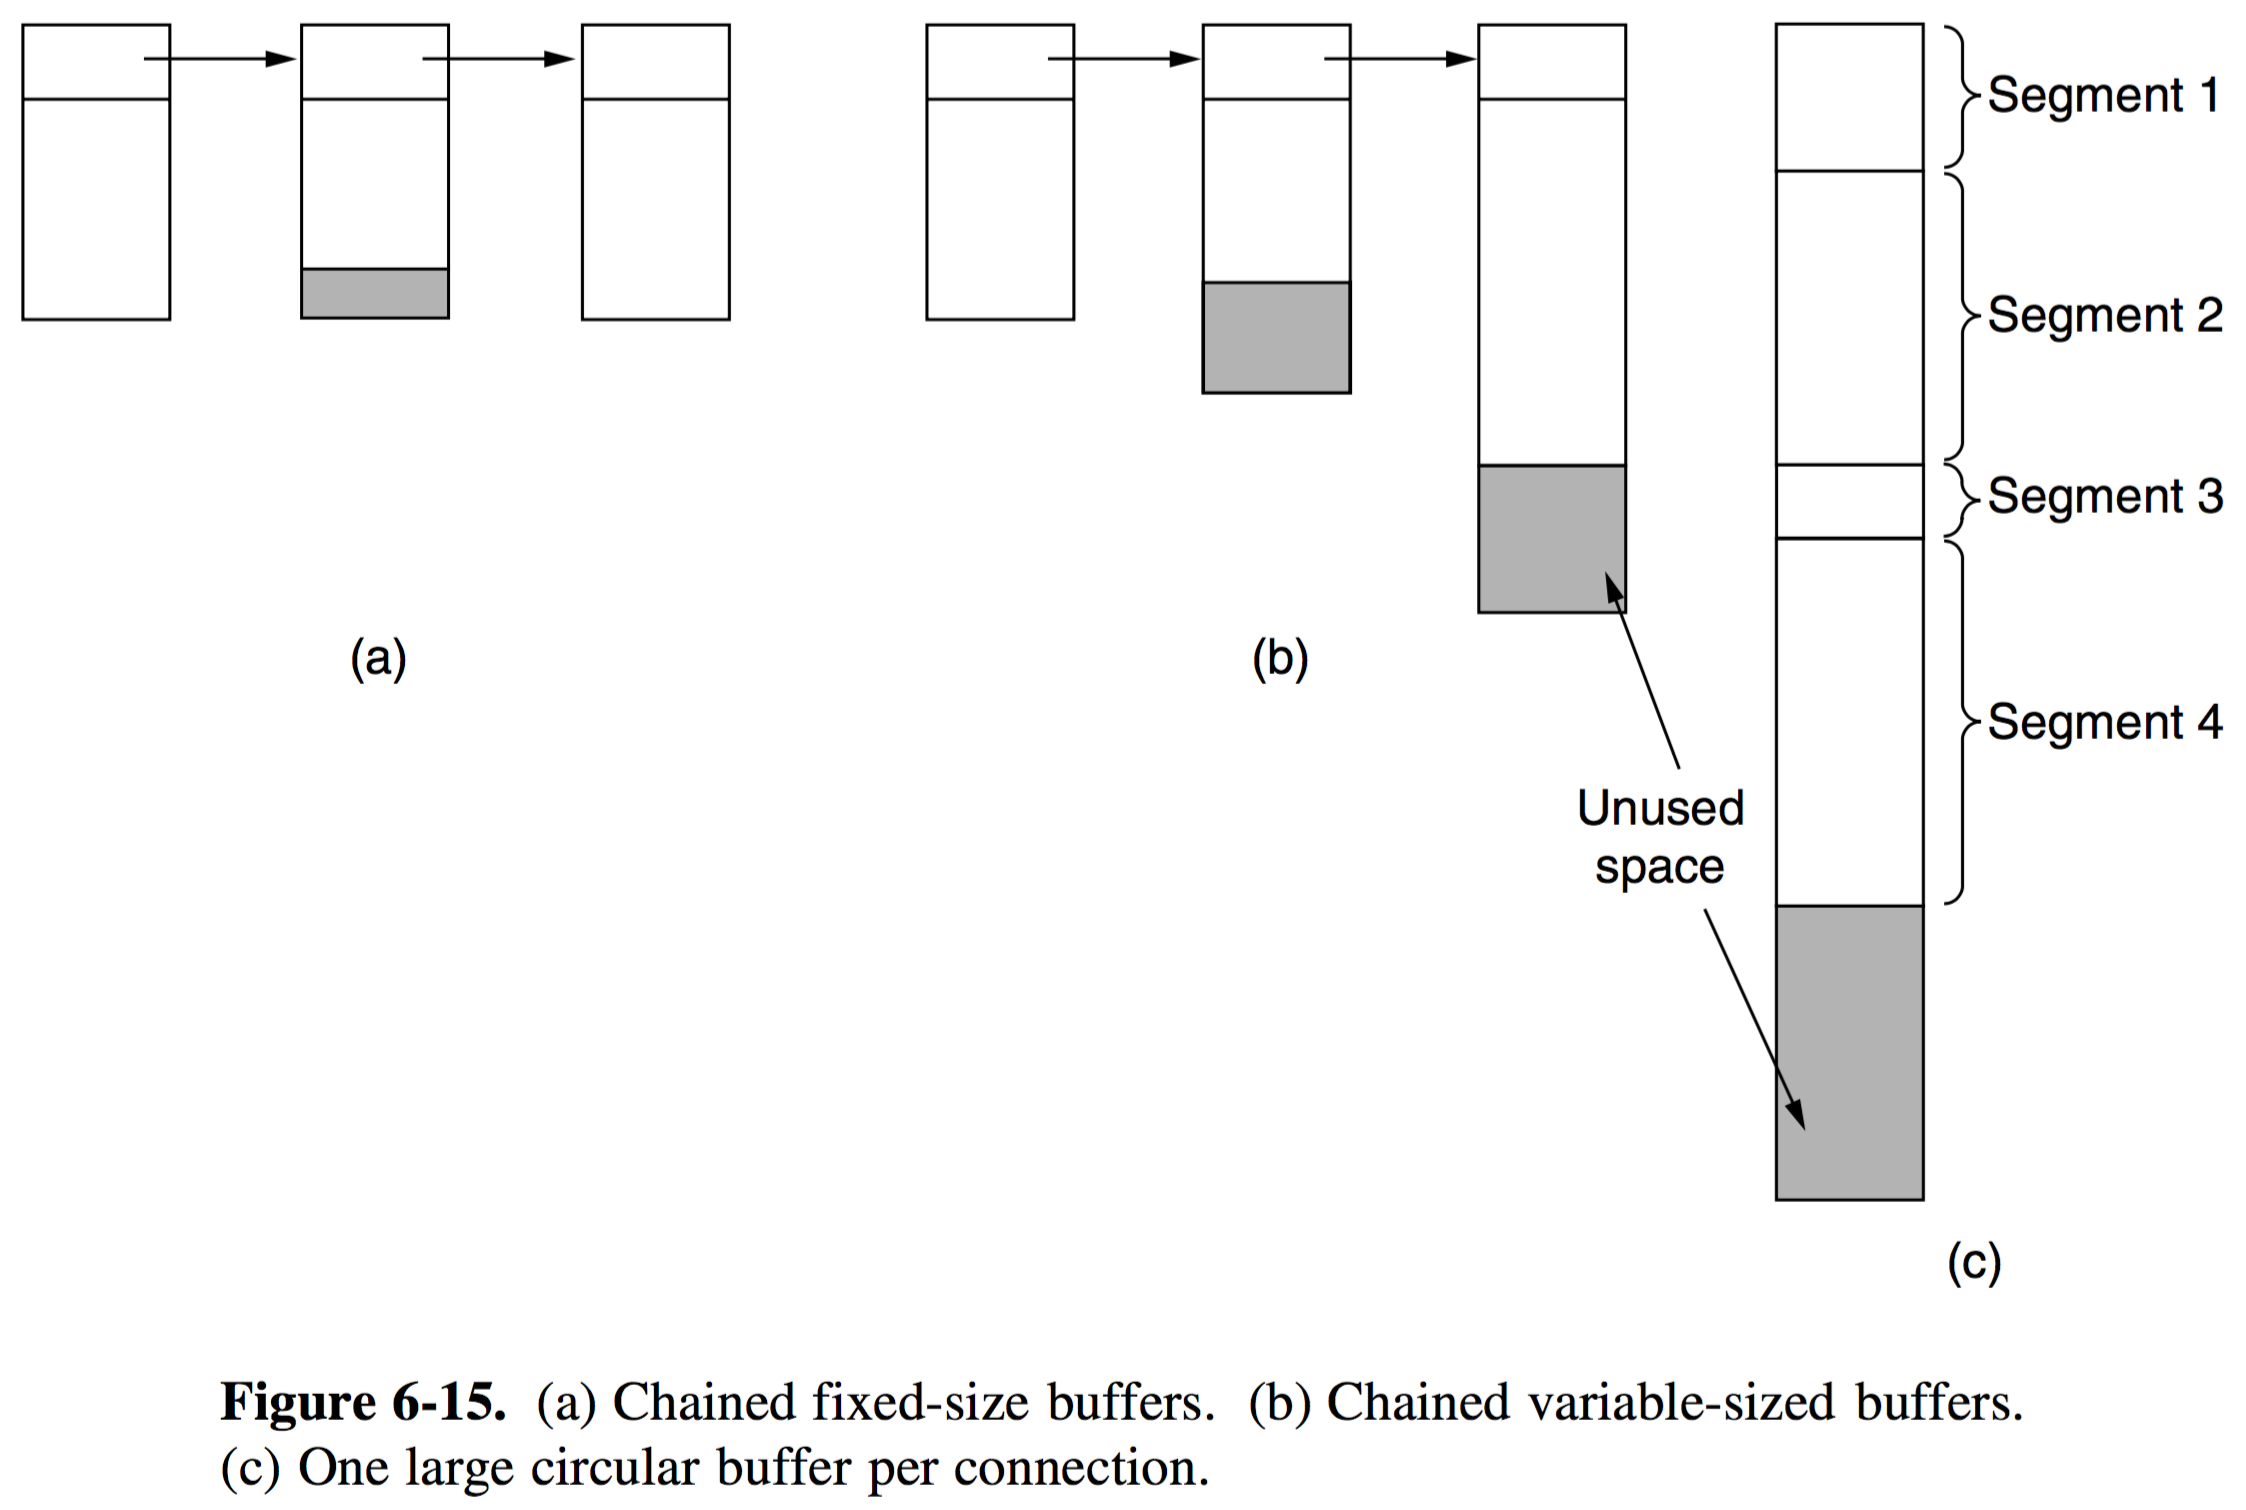
\includegraphics[width=9cm, height=6cm]{./imagenes/bufer.png} 
	\end{center}
	
	\par El equilibrio óptimo entre el almacenamiento en búfer en el origen y en el destino depende del tipo de tráfico transportado por la conexión. Para un tráfico de bajo ancho de banda con ráfagas, como el producido por una terminal interactiva, es mejor no dedicarle búferes, sino adquirirlos de manera dinámica en ambos extremos. 
	
	\par Dado que el emisor no puede estar seguro que el receptor será capaz de adquirir un búfer, el emisor debe retener una copia del segmento hasta recibir su ACK. Por otro lado, para la transferencia de archivos y otro tráfico de alto ancho de banda, es mejor si el receptor dedica una ventana completa de búferes, para permitir el flujo de datos a máxima velocidad. Además para un tráfico en ráfagas de bajo ancho de banda es mejor mantener búferes en el emisor mientras que para tráfico continuo de alto ancho de banda, es mejor hacerlo en el receptor.
	
\subsubsection{Control de flujo}

	\par El problema aquí es evitar que un emisor rápido desborde a un receptor lento. Para el envío de segmentos el \textit{host emisor} tiene un tamaño de ventana que es la mayor cantidad de datos que pueden ser enviados antes de que llegue una confirmación de recepción. Un \textit{host emisor} puede extraer segmentos a enviar que llenen el tamaño de ventana y transmite una copia de cada segmento. Cada uno de esos segmentos se guarda en búfer por si hace falta retransmitirlo. El \textit{host receptor} debe tener un espacio de búferes para la ventana entera del emisor. Si los segmentos llegan en orden, el receptor los pasa a la aplicación receptora y transmite una confirmación de recepción de los mismos al emisor. Cuando llega la confirmación de recepción el emisor descarta las copias de los segmentos confirmados y transmite el próximo segmento.

	\par A medida que se abren y cierran conexiones, y a medida que cambia el patrón del tráfico, el emisor y el receptor necesitan ajustar dinámicamente sus asignaciones de búferes por lo que el protocolo de transporte debe permitir que un \textit{host emisor} solicite espacio en búfer en el otro extremo. Los búferes podrían repartirse por conexión, o en conjunto, para todas las conexiones en operación entre los dos hosts. Si aumentara la cantidad de conexiones abiertas, podría ser necesario reducir una asignación, por lo que el protocolo debe contemplar esta posibilidad.
	
	\par Inicialmente el emisor solicita una cierta cantidad de búferes, con base en sus necesidades percibidas. El receptor otorga entonces tantos búferes como puede, sabiendo su capacidad de manejo de búferes (pero sin saber el tráfico generado) podría indicar al emisor “te he reservado X búferes”. El receptor entonces incorpora tanto las confirmaciones de recepción como las asignaciones de búfer al tráfico de regreso y lleva la cuenta de su asignación de búferes con el receptor. La asignación de búferes disponibles en el emisor debe disminuir cada vez que el emisor envía un segmento. Si ésta asignación llegase a 0 el emisor debe detenerse por completo.

	
	\begin{center} 
			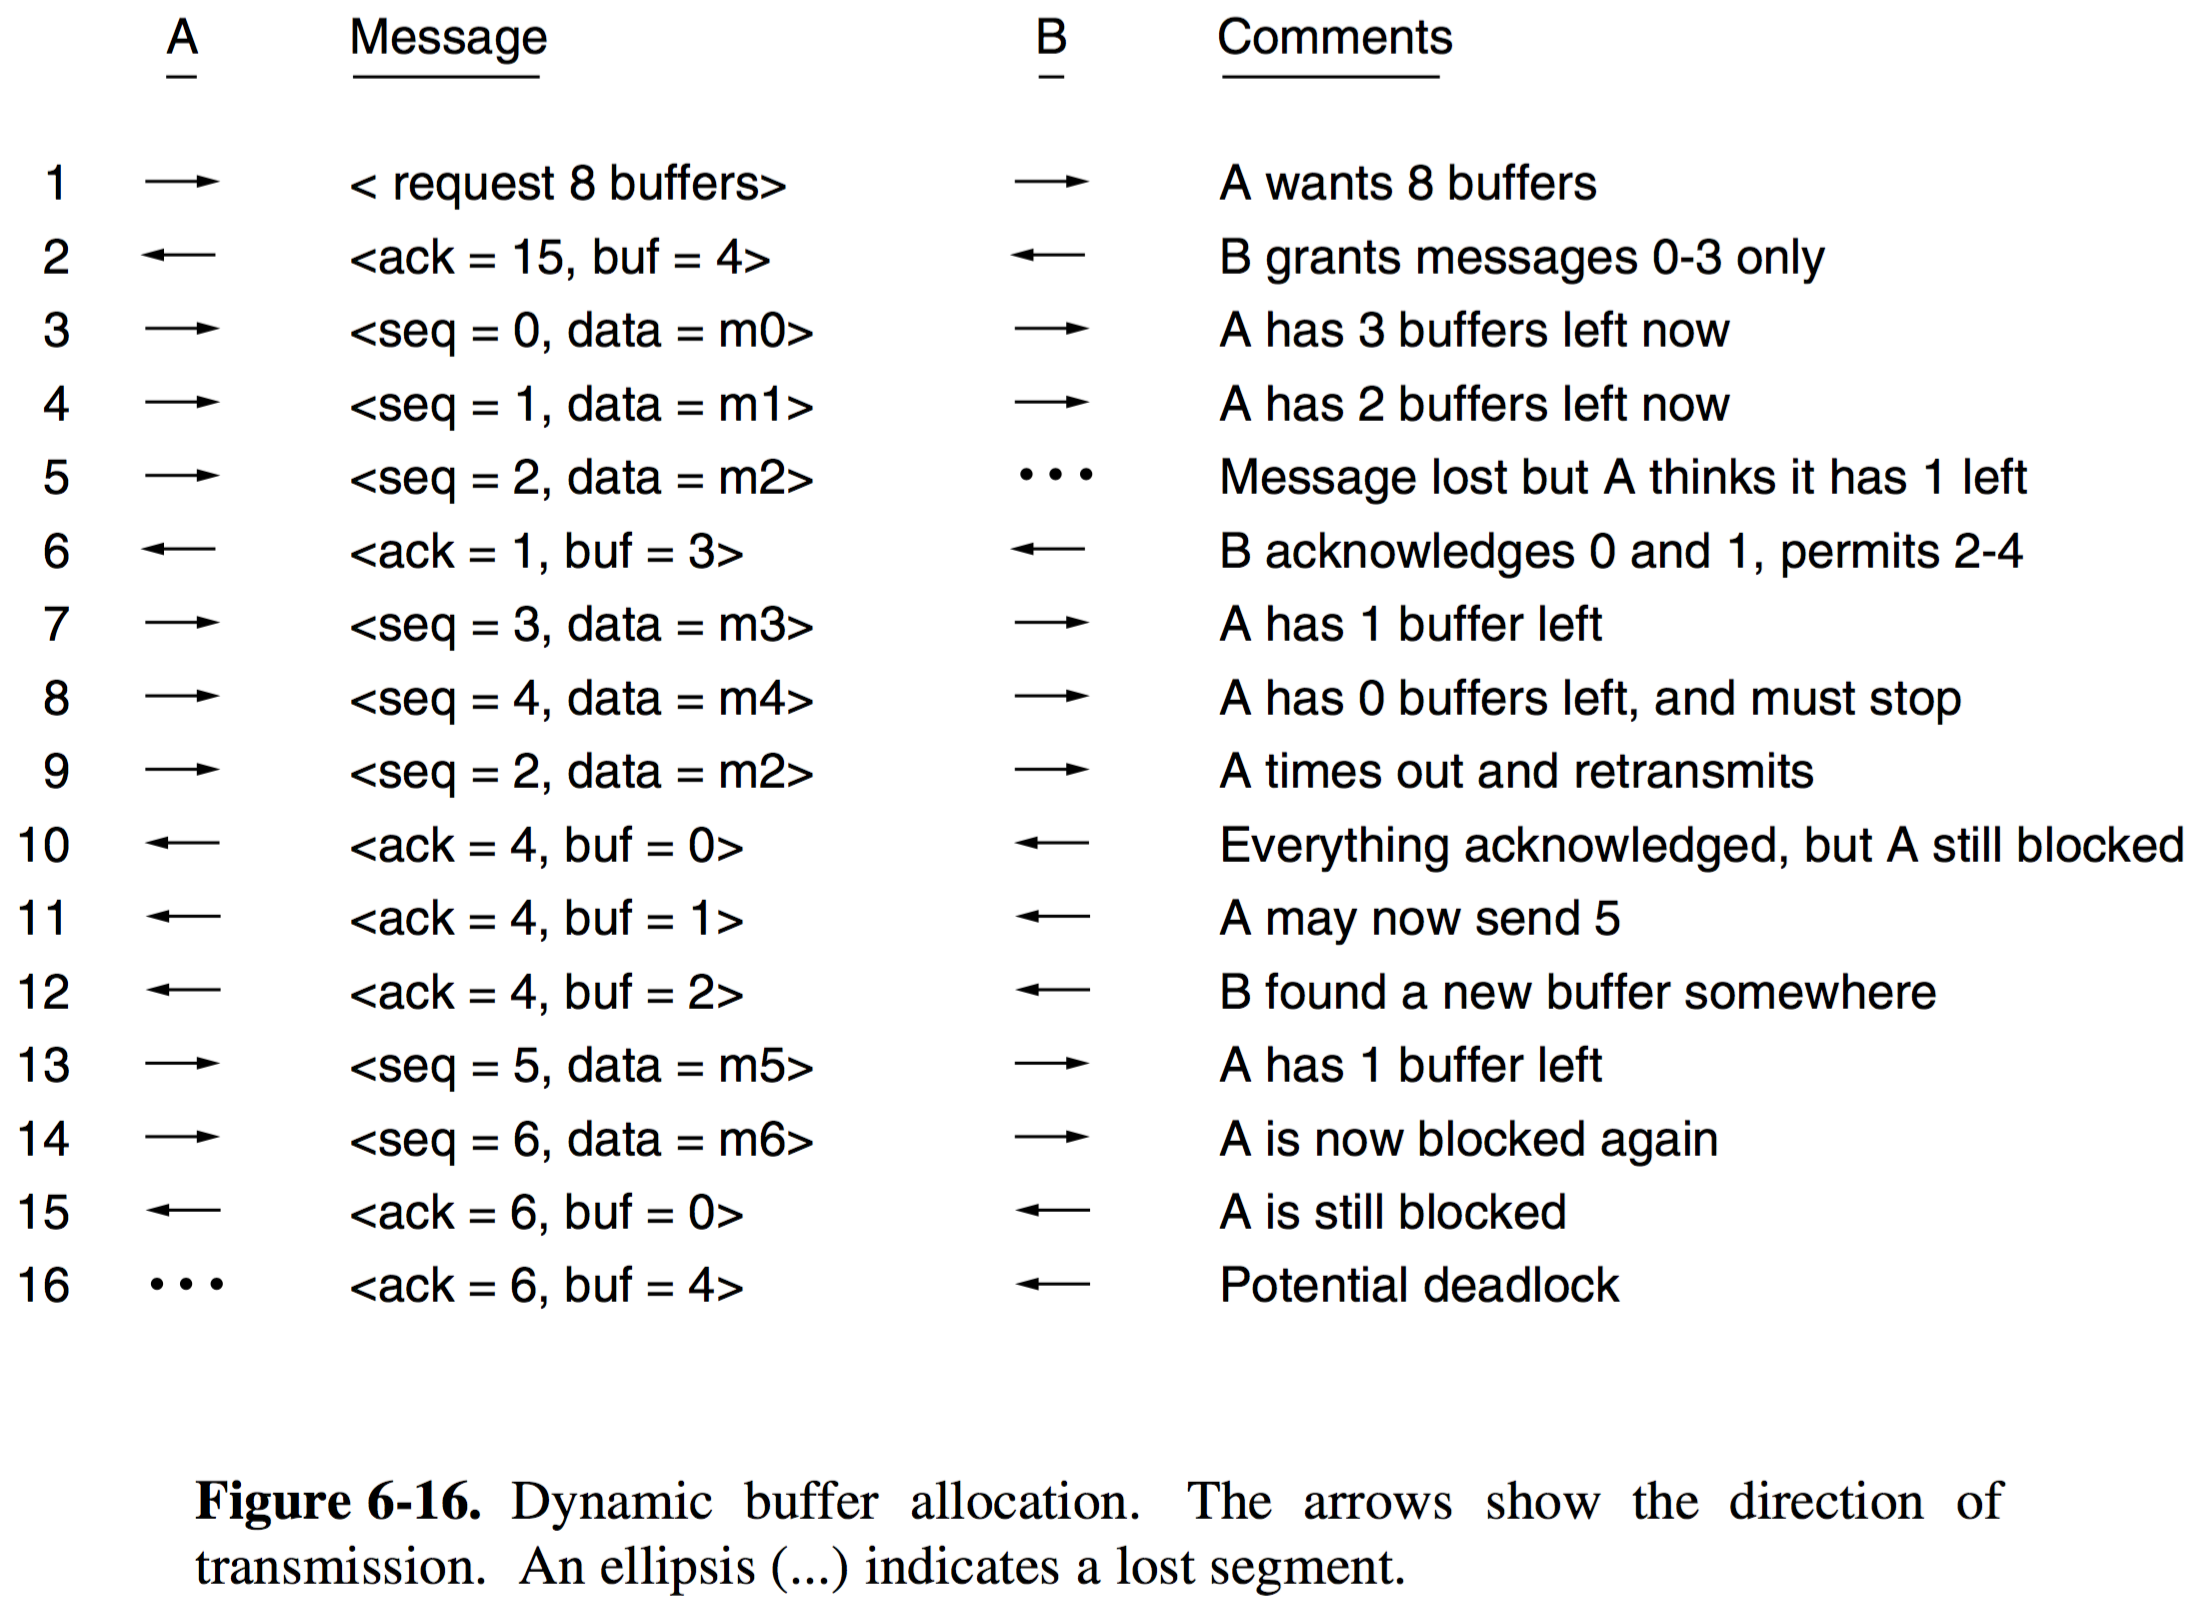
\includegraphics[width=11cm, height=9cm]{./imagenes/flujo.png} 
	\end{center}

\par En la figura 6-16 podemos ver la administración dinámica de ventanas en subred de datagramas con números de secuencia de 4 bits. Supongamos que la información de asignación de búferes viaja en segmentos distintos y no se incorpora en el tráfico de regreso. Inicialmente A quiere 8 búferes, pero se le otorgan solamente 4. Entonces envía 3 segmentos, de los cuales se pierde el tercero. El segmento 6 confirma la recepción de todos los segmentos hasta el número de secuencia 1, inclusive, permitiendo por lo tanto que A libere esos búferes, y además informa a A que tiene permiso de enviar 3 segmentos más comenzando después de 1 (es decir los segmentos 2, 3, y 4). A sabe que ya ha enviado el número 2, por lo que piensa que debe enviar los segmentos 3 y 4, lo que procede a hacer. En este punto se bloquea y debe esperar una nueva asignación de búfer. 

	\par Por otro lado, las retransmisiones inducidas por expiraciones del temporizador (línea 9) sí pueden ocurrir durante el bloqueo, pues usan búferes ya asignados. En la línea 10 B confirma la recepción de todas los segmentos hasta el 4 inclusive, pero se niega a permitir que A continúe. El siguiente segmento de B a A asigna otro búfer y permite a A continuar.

	\par Pueden surgir problemas potenciales con los esquemas de asignación de búferes de este tipo en las subredes de datagramas si hay pérdidas de segmento. Observe la línea 16. B ha asignado ahora más búferes a A, pero el segmento de asignación se perdió. Dado que los segmentos de control no están en secuencia, A se encuentra estancado. Para evitar esta situación cada \textit{host} debe enviar periódicamente un segmento de control con la confirmación de recepción y estado de búferes de cada conexión, de esta manera el estancamiento se romperá tarde o temprano.

\subsection{Recuperación de caídas}

	\par Si los \textit{hosts} y los enrutadores están sujetos a fallas o las conexiones son de larga duración (por ejemplo, descargas extensas de software o medios), la recuperación de estas fallas se vuelve un tema importante. Si la entidad de transporte está totalmente dentro de los \textit{hosts}, la recuperación de fallas de la red y de los enrutadores es sencilla. Las entidades de transporte esperan la pérdida de segmentos todo el tiempo y saben cómo lidiar con esto mediante el uso de retransmisiones.

	\par Un problema más complicado es cómo recuperarse de las fallas del \textit{host}. En particular, tal vez sea conveniente que los clientes sean capaces de continuar trabajando cuando los servidores fallan y se reinician muy rápido. Supongamos que un \textit{host}, el cliente, envía un archivo grande a otro \textit{host}, el servidor de archivos, mediante el uso de un protocolo simple de parada y espera. La capa de transporte en el servidor simplemente pasa los segmentos entrantes al usuario de transporte, uno por uno. De pronto, a mitad de la transmisioón falla el servidor. Al reactivarse, sus tablas se reinicializan, por lo que ya no sabe precisamente en dónde se encontraba.

	\par En un intento por recuperar su estado previo, el servidor podría enviar un segmento de difusión a todos los demás \textit{hosts}, para anunciar que acaba de fallar y solicitar a sus clientes que le informen sobre el estado de todas las conexiones abiertas. Cada cliente puede estar en uno de dos estados: un segmento pendiente (\textit{S1}) o ningún segmento pendiente (\textit{S0}). Con base en esta información de estado, el cliente debe decidir si retransmitirá o no el segmento más reciente.
	
	\par A primera vista parecería obvio: el cliente debe retransmitir sólo si tiene un segmento pendiente sin confirmación de recepción al momento de enterarse de la falla. Sin embargo, una inspección más cercana revela dificultades con esta metodología ingenua. Considere, por ejemplo, la situación en la que la entidad de transporte del servidor envía primero una confirmación de recepción y luego, una vez que se envía esta confirmación de recepción, escribe en el proceso de aplicación. Escribir un segmento en el flujo de salida y enviar una confirmación de recepción son dos eventos diferentes que no se pueden hacer al mismo tiempo. Si ocurre una falla después de enviar la confirmación de recepción pero antes de que la escritura se complete, el cliente recibirá la confirmación de recepción y estará por ende en el estado \textit{S0} cuando llegue el anuncio de recuperación de la falla. Entonces el cliente no retransmitirá, pues pensará que llegó el segmento. Esta decisión del cliente provoca que falte un segmento.
	
	\par Podríamos pensar que todo lo que hay que hacer es reprogramar la entidad de transporte para que primero haga la escritura y luego envíe la confirmación de recepción. Imagine que se ha hecho la escritura pero que la falla ocurre antes de enviar la confirmación de recepción. El cliente se encontrará en el estado \textit{S1}, y por tanto retransmitirá, lo que provocará un segmento duplicado sin detectar en el flujo de salida que va al proceso de aplicación del servidor.

	\par Sin importar cómo se programen el emisor y el receptor, siempre hay situaciones en las que el protocolo no se puede recuperar de manera apropiada. Podemos programar el servidor en una de dos formas: enviar confirmación de recepción primero o escribir primero. El cliente se puede programar en una de cuatro formas: siempre retransmitir el último segmento, nunca retransmitir el último segmento, retransmitir sólo en el estado \textit{S0} o retransmitir sólo en el estado \textit{S1}. Esto nos da ocho combinaciones pero, como veremos, para cada combinación existe cierto conjunto de eventos que hacen fallar al protocolo.

	\par Son posibles tres eventos en el servidor: enviar una confirmación de recepción (A), escribir al proceso de salida (W) y fallar (C). Los tres eventos pueden ocurrir en seis órdenes diferentes: AC(W), AWC, C(AW), C(WA), WAC y WC(A), donde los paréntesis se usan para indicar que ni A ni W pueden ir después de C (es decir, una vez que el servidor falla, así se queda). En la figura 6-18 se muestran las ocho combinaciones de las estrategias de cliente y servidor, junto con las secuencias de eventos válidas para cada una. Observe que para cada estrategia hay alguna secuencia de eventos que provoca que el protocolo falle. Por ejemplo, si el cliente siempre retransmite, el evento AWC generará un duplicado no detectado, incluso aunque los otros dos eventos funcionen de manera apropiada.
	
	\begin{center}
		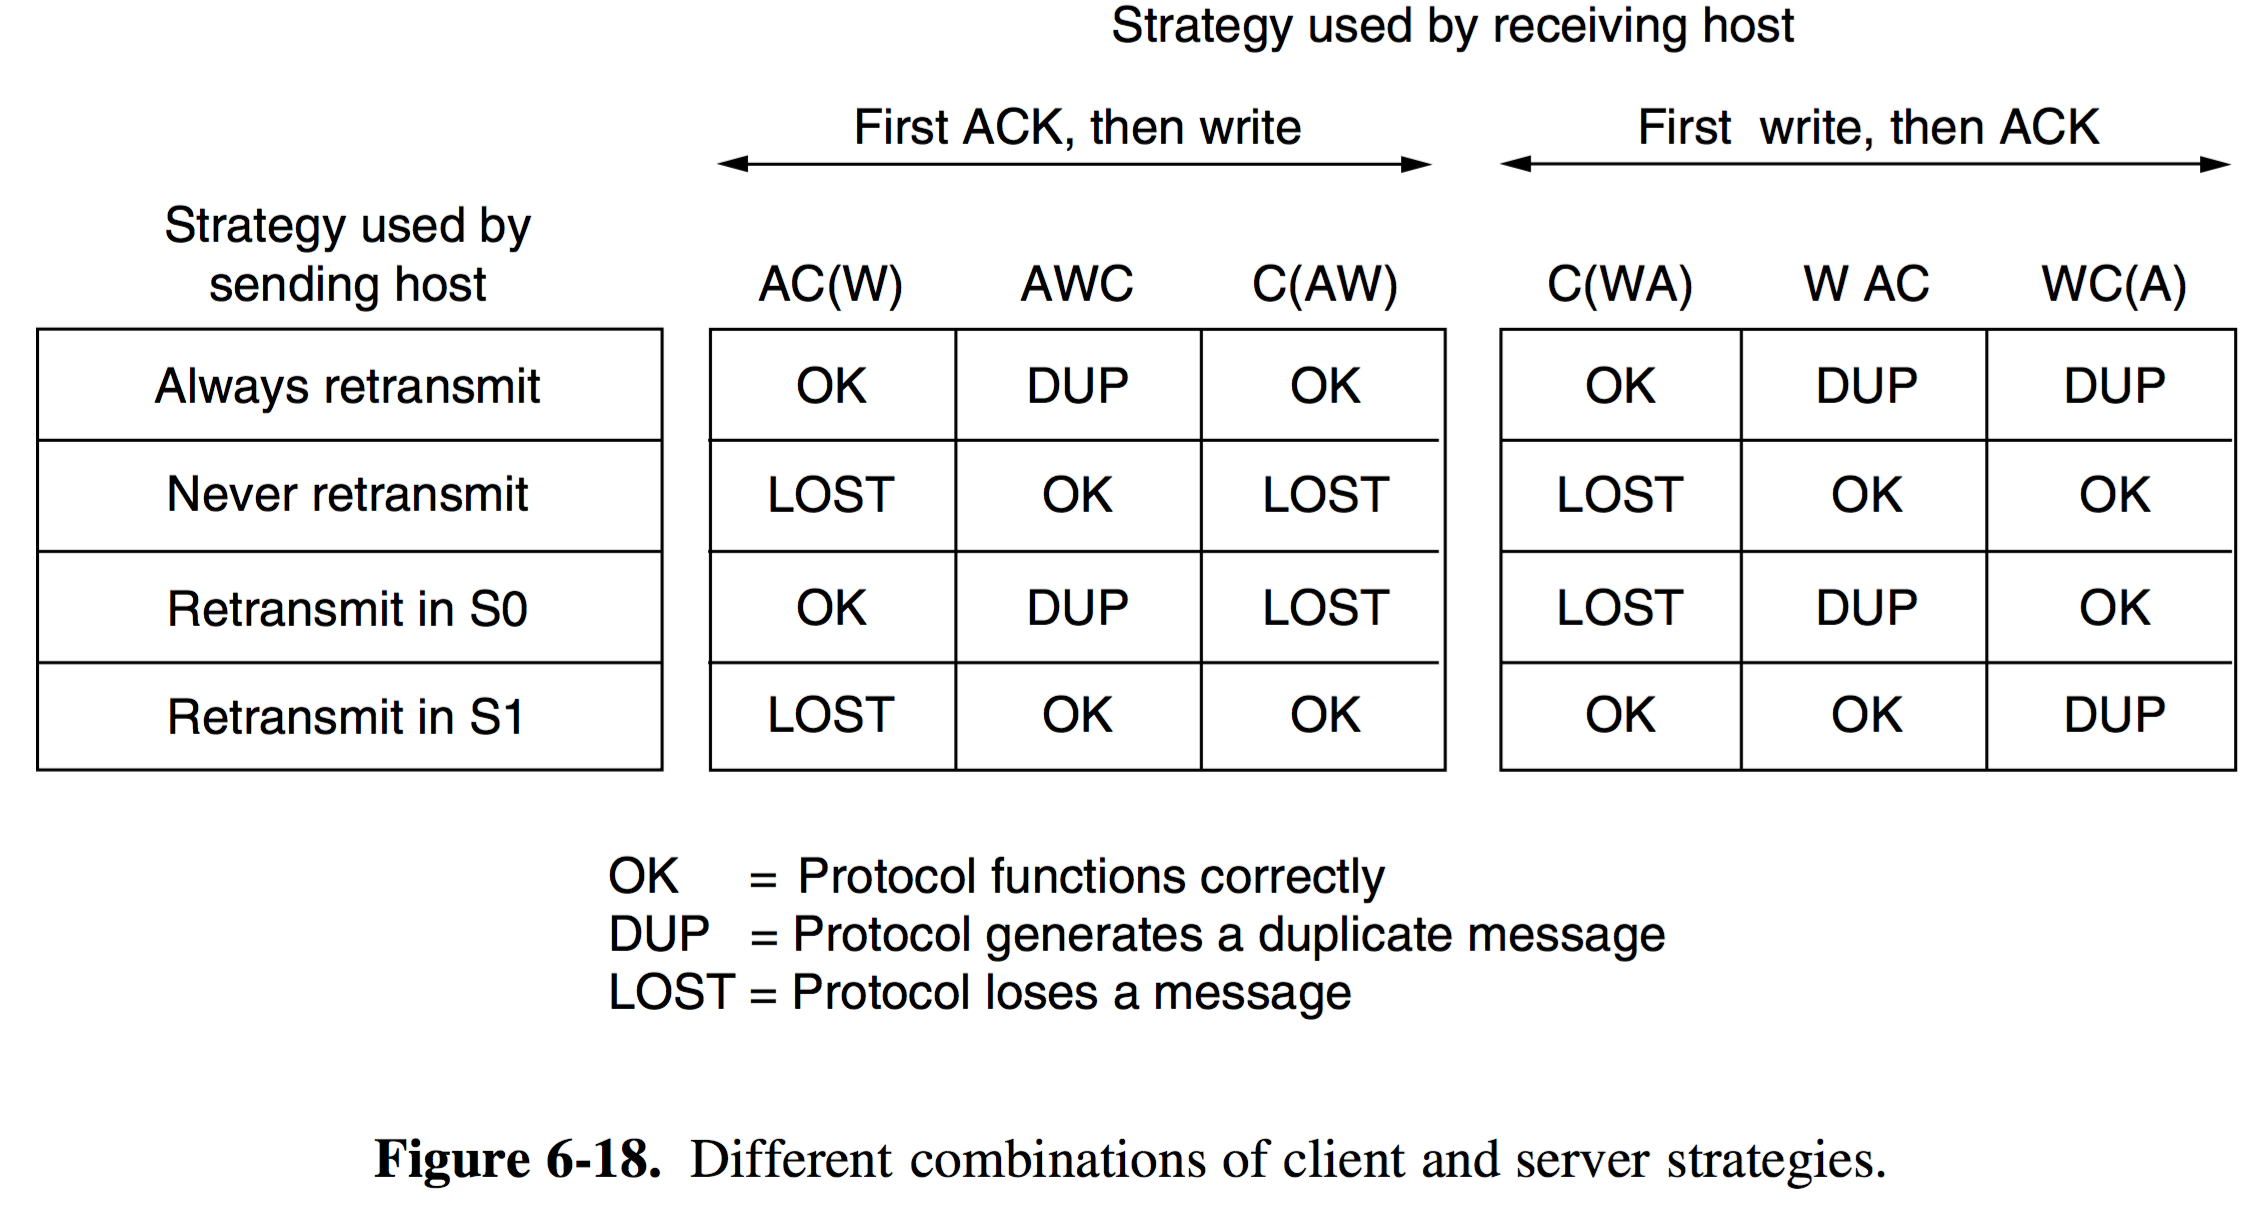
\includegraphics[width=11cm, height=7cm]{./imagenes/fallas.png} 
	\end{center}

	\par Hacer más elaborado el protocolo no sirve de nada. Aunque el cliente y el servidor intercambien varios segmentos antes de que el servidor intente escribir, para que el cliente sepa con exactitud lo que está a punto de ocurrir, el cliente no tiene manera de saber si ha ocurrido una falla justo antes o justo después de la escritura. La conclusión es inevitable: según nuestra regla básica de que no debe haber eventos simultáneos (es decir, que eventos separados ocurren uno después de otro y no al mismo tiempo), la falla de un \textit{host} y su recuperación no pueden hacerse transparentes a las capas superiores.

	\par Dicho en términos más generales, podemos replantear este resultado como “la recuperación de una falla en la \textit{capa N} se la se puede llevar a cabo en la \textit{capa N + 1}”, y esto es sólo si la capa superior retiene suficiente información del estado como para reconstruir la condición en la que se encontraba antes de que ocurriera el problema. Esto es consistente con el caso que mencionamos antes, en el que la capa de transporte puede recuperarse de fallas en la capa de red, siempre y cuando cada extremo de una conexión lleve el registro del estado en el que se encuentra.	
	
	\par Considere el caso de un usuario que introduce solicitudes de transacciones para una base de datos remota. Suponga que la entidad de transporte remota está programada para pasar primero los segmentos a la siguiente capa superior y luego emitir las confirmaciones de recepción. Incluso en este caso, el hecho de que la máquina de un usuario reciba una confirmación de recepción no significa necesariamente que el \textit{host} remoto se quedó encendido el tiempo suficiente como para actualizar la base de datos. Quizá es imposible lograr una verdadera confirmación de recepción de extremo a extremo, en donde si se recibe significa que en realidad se hizo el trabajo y, si no se recibe, significa que no se realizó el trabajo.

\subsection{Control de congestión}

	\par Como va bajando significativamente el precio de la memoria eventualmente se podrá equipar a los \textit{hosts} con tanta memoria que la falta de búferes dejará de ser un problema. Si el tamaño de búfer ya no limita el flujo máximo, aparecerá otro cuello de botella: la \textit{capacidad de carga de la subred}. Si enrutadores adyacentes pueden intercambiar como mucho \textit{X paquetes/seg} y hay \textit{K} trayectorias sin traslape entre un par de \textit{hosts}, no hay manera de que esos \textit{hosts} puedan intercambiar más de \textit{$K * X $  TPDUs/seg}, sin importar la cantidad de espacio de búfer disponible en cada terminal.

	\par Si el emisor presiona demasiado (es decir, envía más que \textit{$K * X $  TPDU s/seg}), la subred se congestionará, pues será incapaz de entregar las TPDUs a la velocidad con que llegan. Lo que se necesita es un mecanismo basado en la capacidad de carga de la subred en lugar de la capacidad de almacenamiento en búfer del receptor. Es claro que el mecanismo de control de flujo debe aplicarse al emisor para evitar que estén pendientes demasiadas TPDUs sin confirmaciones de recepción al mismo tiempo.

	\par Belsens propuso el uso de un esquema de control de flujo de ventana corrediza en el que el emisor ajusta dinámicamente el tamaño de la ventana para igualarla a la capacidad de carga de la red. Si la red puede manejar \textit{C segmentos/seg} y el tiempo de ciclo (incluidos transmisión, propagación, encolamiento, procesamiento en el receptor y devolución de la confirmación de recepción) es de \textit{R}, entonces la ventana del emisor debe ser de \textit{$C * R$}. Con una ventana de este tamaño, el emisor normalmente opera con el canal a su máxima capacidad. Cualquier pequeña disminución en el desempeño de la red causará que se bloquee.

	\par A fin de ajustar periódicamente el tamaño de la ventana, el emisor podría vigilar ambos parámetros y calcular después el tamaño de ventana deseado. La capacidad de carga puede determinarse con solo contar la cantidad de segmentos confirmados durante algún período y dividirla entre el período. Durante la medición el emisor debe enviar a la mayor velocidad posible, para asegurarse que sea la capacidad de carga de la red, y no la baja tasa de entrada el factor limitante de la tasa de confirmaciones de recepción. El tiempo requerido para la confirmación de recepción de un segmento transmitido puede medirse exactamente y mantenerse una media de operación. Dado que la capacidad de la red depende de la cantidad de tráfico en ella, debe ajustarse el tamaño de la ventana con frecuencia para responder a los cambios en la capacidad de carga.

\section{Los protocolos de transporte de internet: UDP}
	\par Internet tiene dos protocolos principales en la capa de transporte, uno sin conexión y otro orientado a la conexión. Los protocolos se complementan entre sí. El protocolo sin conexión es UDP. Prácticamente no hace nada más que enviar paquetes entre aplicaciones, y deja que las aplicaciones construyan sus propios protocolos en la parte superior según sea necesario. El protocolo orientado a conexión es TCP. Hace casi todo. Realiza las conexiones y agrega confiabilidad mediante las retransmisiones, junto con el control de flujo y el control de congestión, todo en beneficio de las aplicaciones que lo utilizan.

\subsection{Introducción a UDP}

	\par UDP llamado Protocolo de Datagrama de Usuario (\textbf{Use Datagram Protocol}) es un protocolo de transporte no orientado a la conexión. UDP proporciona una forma para que las aplicaciones envíen datagramas IP encapsulados sin tener que establecer una conexión.
	
	\par UDP transmite segmentos que consisten en un encabezado de 8 bytes seguido de la carga útil. En la figura 6-27 se muestra ese encabezado. Los dos puertos sirven para identificar los puntos terminales dentro de las máquinas de origen y destino. Cuando llega un paquete UDP, su carga útil se entrega al proceso que está conectado al puerto de destino. Este enlace ocurre cuando se utiliza la primitiva BIND o algo similar.
	
	\par El valor principal de contar con UDP en lugar de simplemente utilizar IP puro es la adición de los puertos de origen y destino. Sin los campos de puerto, la capa de transporte no sabría qué hacer con cada paquete entrante. Con ellos, entrega el segmento incrustado a la aplicación correcta.
	
	\begin{center}
		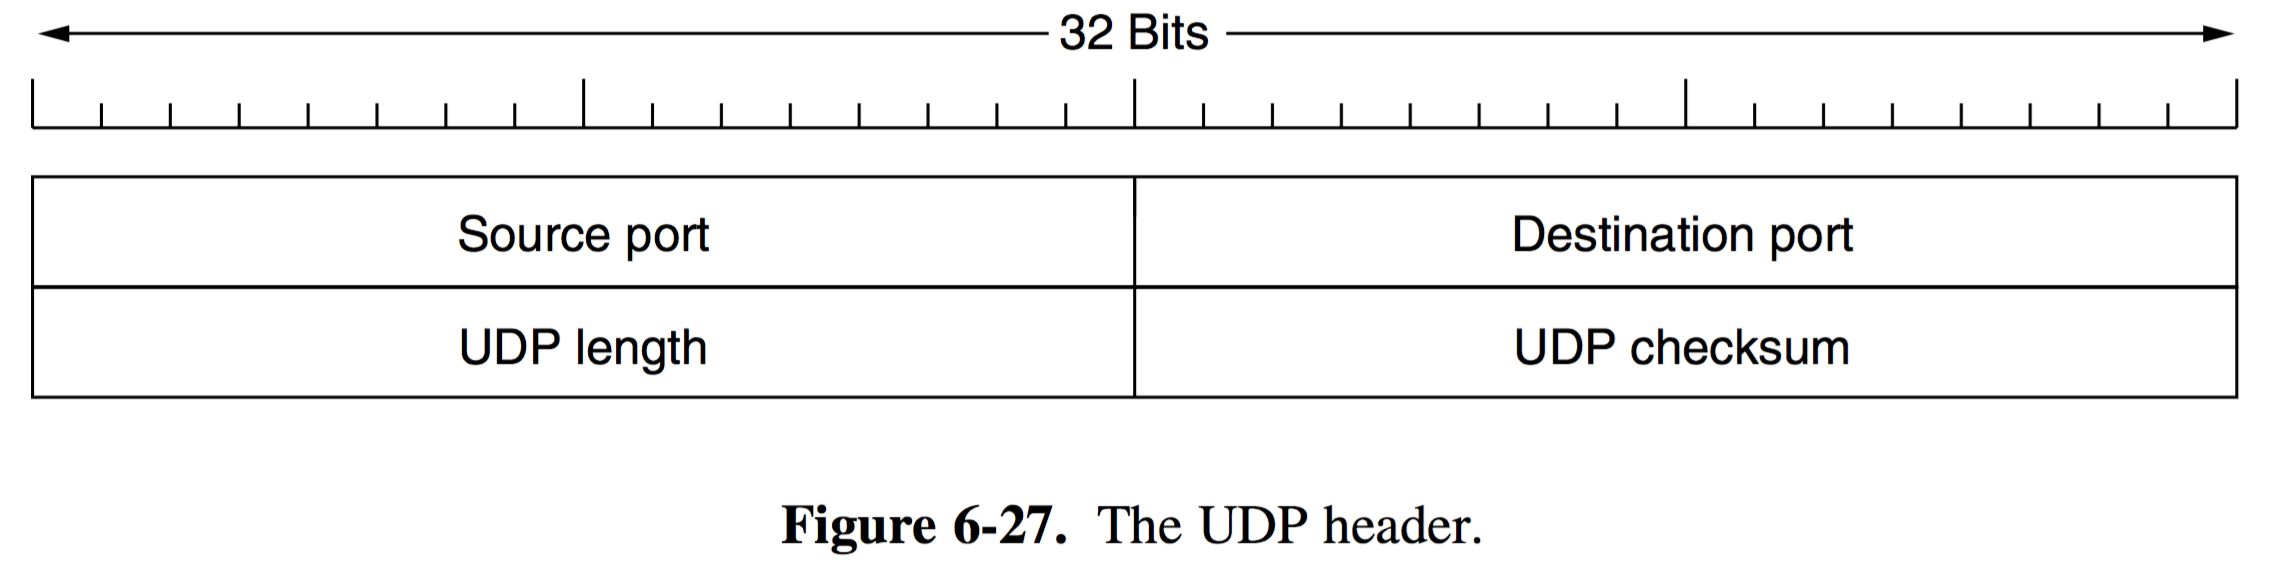
\includegraphics[width=10cm, height=4cm]{./imagenes/udp.png} 
	\end{center}
	
	\par El puerto de origen se necesita principalmente cuando hay que enviar una respuesta al origen. Al copiar el campo \textit{Puerto de origen} del segmento entrante en el campo \textit{Puerto de destino} del segmento que sale, el proceso que envía la respuesta puede especificar cuál proceso de la máquina emisora va a recibirlo.

	\par El campo \textit{Longitud UDP} incluye el encabezado de 8 bytes y los datos, mientras que el campo \textit{Suma de verificación} es opcional y se almacena como 0 si no se calcula (un 0 calculado se almacena como 1s). Su desactivación no tiene sentido a menos que la calidad del servicio de los datos no importe (por ejemplo, en la voz digitalizada).
	
	\par UDP no realiza control de flujo, control de congestión o retransmisión cuando se recibe un segmento erróneo. Todo lo anterior le corresponde a los procesos de usuario. 
	
	\par UDP es especialmente útil es en las situaciones cliente-servidor. Con frecuencia, el cliente envía una solicitud corta al servidor y espera una respuesta corta. Si se pierde la solicitud o la respuesta, el cliente simplemente puede esperar a que expire su temporizador e intentar de nuevo. El código no sólo es simple, sino que se requieren menos mensajes (uno en cada dirección) en comparación con un protocolo que requiere una configuración inicial, como TCP.

	\par Una aplicación que utiliza de esta manera a UDP es DNS (Domain Name System), un programa que necesita buscar la dirección IP de algún host puede enviar al servidor DNS un paquete UDP que contenga el nombre de dicho host. El servidor responde con un paquete UDP que contiene la dirección IP del host. No se necesita configuración por adelantado ni tampoco una liberación posterior. Sólo dos mensajes que viajan a través de la red.
	
\subsection{RPC: Llamada a procedimiento remoto}

	\par Enviar un mensaje a un host remoto y obtener una respuesta es muy parecido a realizar la llamada a una función en un lenguaje de programación. Así las interacciones de solicitud-respuesta en las redes se asignan en forma de llamadas a procedimientos, de este modo las aplicaciones de red son mucho más fáciles de programar y de manejar.
	
	\par Cuando un proceso en la \textit{máquina 1} llama a otro procedimiento en la \textit{máquina 2}, el proceso invocador en \#1 se suspende y la ejecución del procedimiento invocado se lleva a cabo en la \textit{máquina 2}. Se puede transportar información del proceso invocador al proceso invocado en los parámetros, y se puede regresar información en el resultado del procedimiento. El paso de mensajes es transparente para el programador. Esta técnica se conoce como RPC (\textbf{Remote Procedure Call}).

	\par El objetivo de RPC es hacer que una llamada a procedimiento remoto sea lo más parecida posible a una local. Para llamar a un procedimiento remoto, el programa cliente se debe enlazar con un pequeño procedimiento de biblioteca, llamado \textbf{stub del cliente}, que representa al procedimiento servidor en el espacio de direcciones del cliente. Asimismo, el servidor se enlaza con una llamada a procedimiento denominada \textbf{stub del servidor}. Estos procedimientos ocultan el hecho de que la llamada a procedimiento del cliente al servidor no es local. En la figura 6-29 se muestran los pasos reales para realizar una RPC.
	
	\begin{center}
		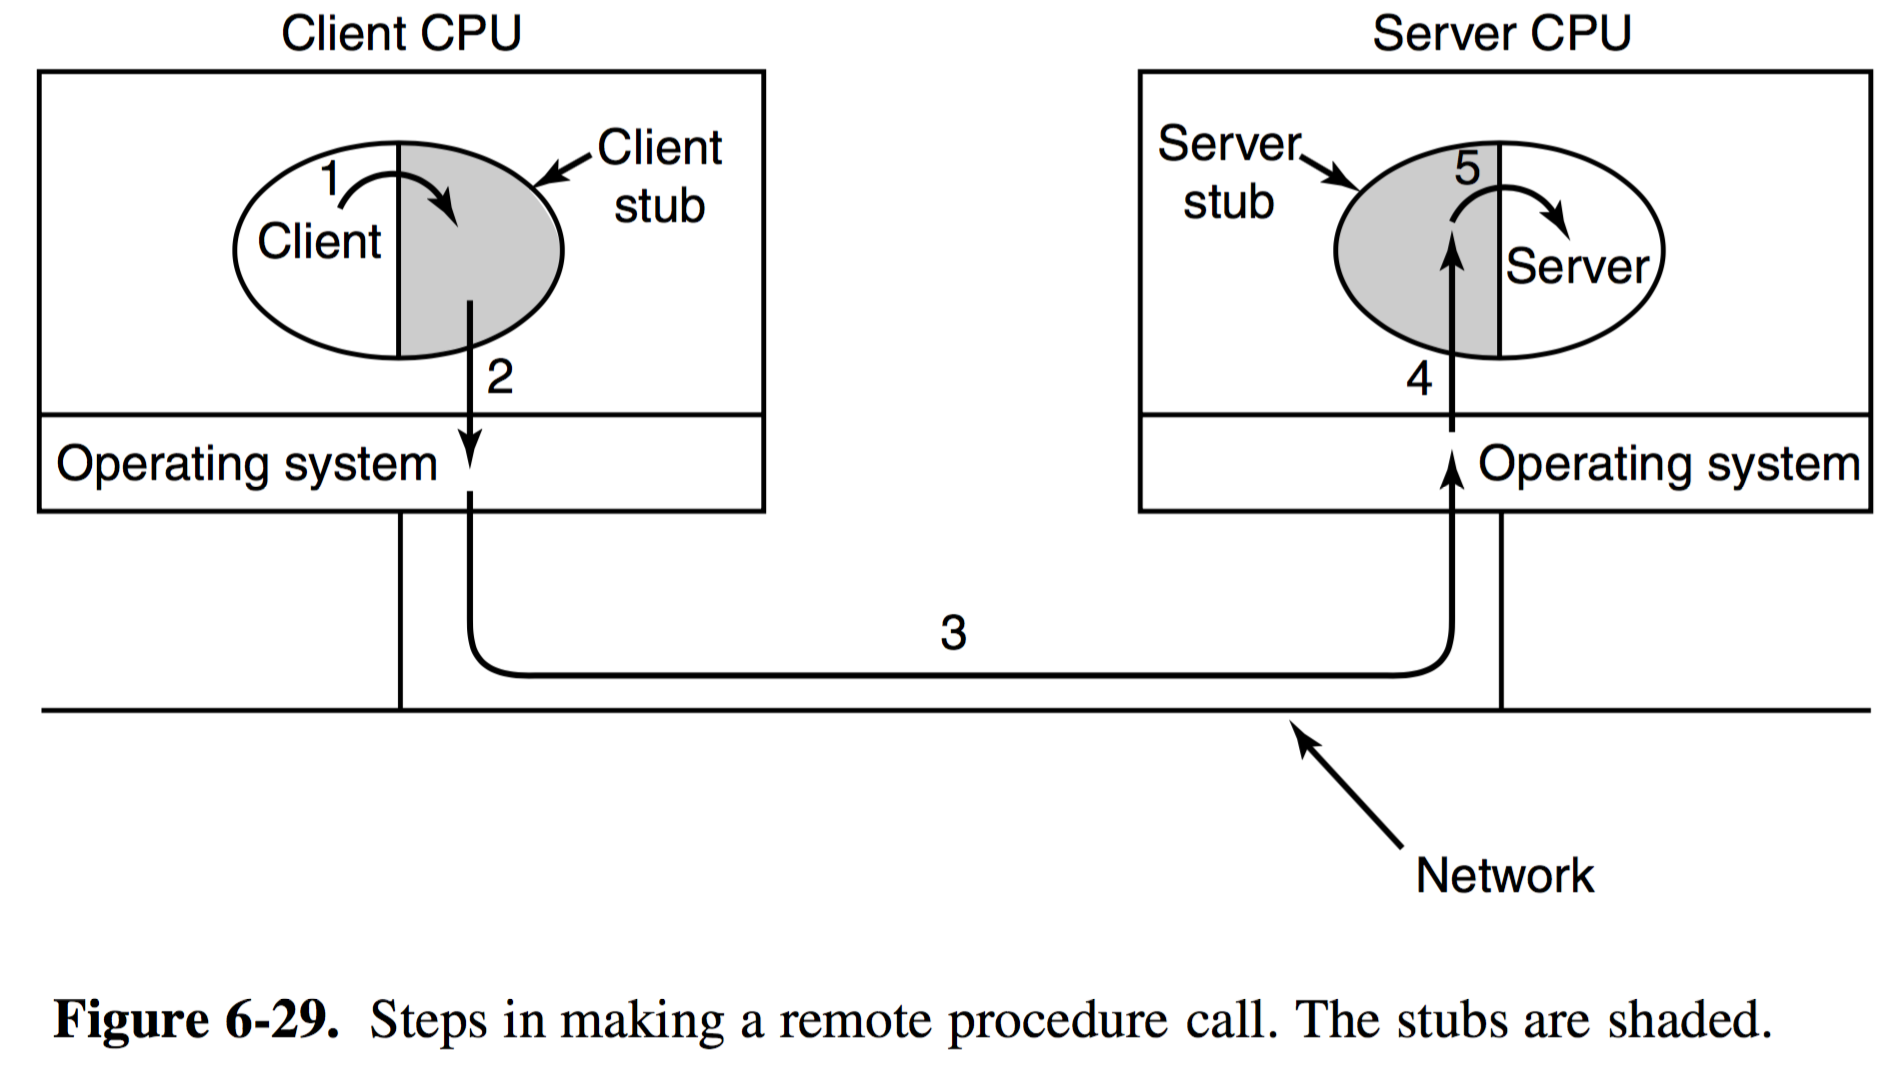
\includegraphics[width=10cm, height=4cm]{./imagenes/rpc.png} 
	\end{center}
	
	\begin{enumerate}
		\item El cliente llama al \textbf{stub del cliente}. Ésta es una llamada a procedimiento local, y los parámetros se meten en la pila de la forma tradicional.
		\item El \textbf{stub del cliente} empaca los parámetros en un mensaje y realiza una llamada de sistema para enviar el mensaje, a este proceso se lo conoce como \textit{marshaling} (empaquetar).
		\item El sistema operativo envía el mensaje de la máquina cliente a la máquina servidor.
		\item El sistema operativo pasa el paquete entrante al \textbf{stub del servidor}. 
		\item El \textbf{stub del servidor} llama al procedimiento servidor con los parámetros sin empacar (\textit{unmarshaling}).
		\item La respuesta sigue la misma ruta en la dirección opuesta.
	\end{enumerate}
	
	\par El procedimiento cliente realiza una llamada a procedimiento normal local al \textbf{stub del cliente} la cual tiene el mismo nombre que el procedimiento en el servidor.
	
	\par A pesar de la elegancia conceptual de RPC, hay alguna desventajas ocultas. Con RPC el paso de punteros es imposible ya que el cliente y el servidor están en diferentes espacios de direcciones. Por lo general los procedimientos invocador e invocado pueden comunicarse por el uso de variables globales y parámetros. Si el procedimiento invocado se mueve a una máquina remota, el código fallará porque las variables globales ya no se pueden compartir.


	\par RPC y UDP son una buena combinación y RPC se usa comúnmente con UDP.  Cuando los parámetros o resultados sean más grandes que el tamaño máximo del paquete UDP, tal vez sea necesario establecer una conexión TCP y enviar una solicitud a través de ella.

\subsection{Protocolos de transporte en tiempo real}

	\par UDP también se utiliza en aplicaciónes de tiempo real como la radio en Internet, la telefonía en Internet, la música bajo demanda, las videoconferencias, el video bajo demanda y otras aplicaciones multimedia que se han vuelto más comunes. Las personas descubrieron que cada una de esas aplicaciones estaba reinventando más o menos el mismo protocolo de transporte de tiempo real. Cada vez era más claro que tener un protocolo genérico de transporte en tiempo real para múltiples aplicaciones sería una excelente idea.

	\par A raíz de esto fue que nació el RTP (\textbf{Real-time Transport Protocol}), utilizado ampliamente para aplicaciones multimedia. RTP se ejecuta en espacio de usuario sobre UDP (en el sistema operativo). La aplicación multimedia consiste en múltiples flujos de audio, video, texto y quizás otros flujos. Éstos se colocan en la biblioteca RTP, la cual está en el espacio de usuario junto con la aplicación. Esta biblioteca multiplexa los flujos y los codifica en paquetes RTP, que después coloca en un socket. En el extremo del socket correspondiente al sistema operativo, se generan paquetes UDP para envolver los paquetes RTP y se entregan al IP para que los transmita a través de un enlace tal como Ethernet. En la figura 6-30(a) se muestra la pila de protocolos para esta situación. En la figura 6-30(b) se muestra el anidamiento de paquetes.
	
	\begin{center}
		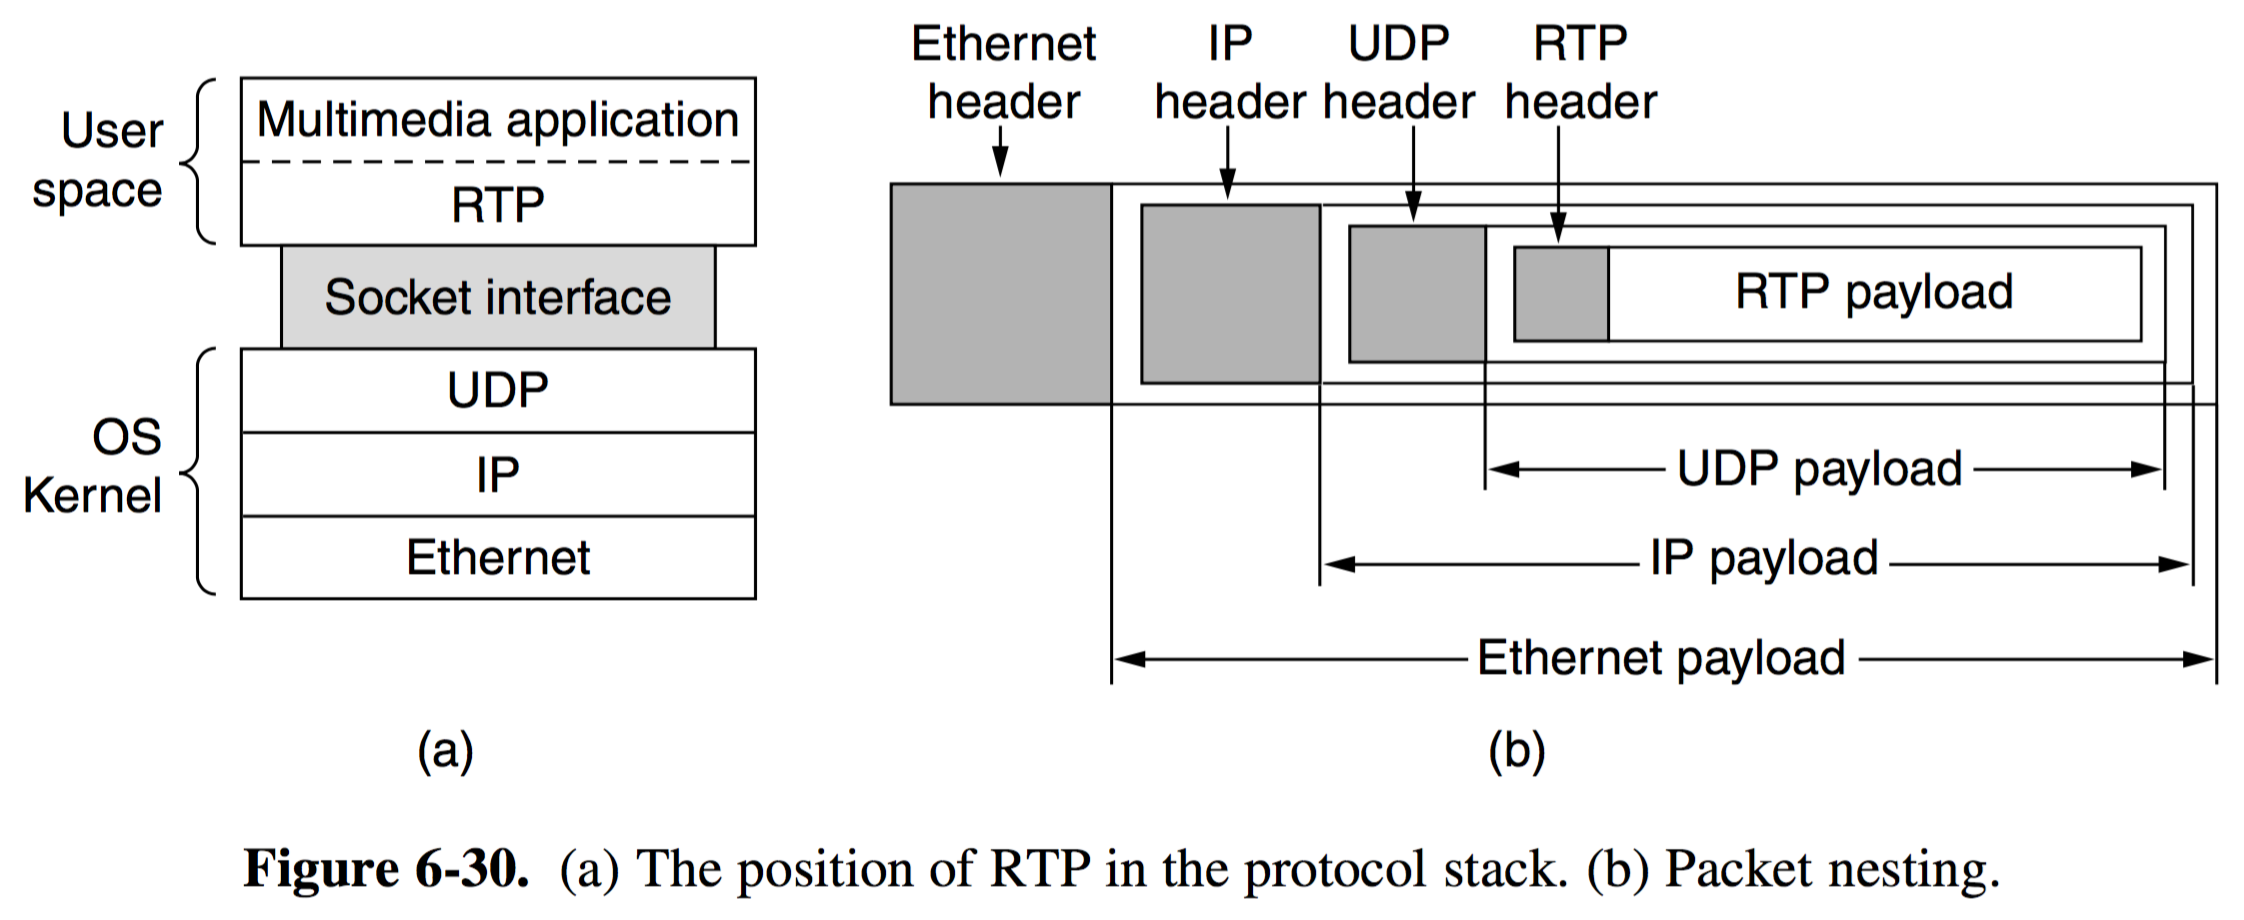
\includegraphics[width=12cm, height=6cm]{./imagenes/tiemporeal.png} 
	\end{center}

\subsubsection{RTP: Protocolo de Transporte en Tiempo Real}

	\par La función de RTP es multiplexar varios flujos de datos de tiempo real en un solo flujo de paquetes UDP. El flujo UDP se puede enviar a un solo destino (\textbf{unidifusión}) o a múltiples destinos (\textbf{multidifusión}). No hay garantías especiales acerca de la entrega, así que los paquetes se pueden perder, retrasar, corromper, etc.
		
	\par A cada paquete enviado en un flujo RTP se le da un número más grande que a su predecesor. Esta numeración permite al destino determinar si falta algún paquete en cuyo caso, la mejor acción a realizar queda a criterio de la aplicación. Tal vez esta acción sea omitir una trama de video si los paquetes transportan datos de video, o aproximar el valor faltante mediante la interpolación en caso de que los paquetes transporten datos de audio. La retransmisión no es una opción práctica debido a la probabilidad de que el paquete retransmitido llegue muy tarde como para ser útil por lo que RTP no tiene confirmaciones de recepción ni ningún mecanismo para solicitar retransmisiones.

	\par Las estampas de tiempo (\textit{time stamping}) son otra herramienta que muchas de las aplicaciones en tiempo real necesitan. La idea aquí es permitir que la fuente asocie una estampa de tiempo con la primera muestra de cada paquete. Las estampas de tiempo son relativas al inicio del flujo, por lo que sólo son importantes las diferencias entre dichas estampas. Como veremos en breve, este mecanismo permite que el destino haga un uso muy moderado del almacenamiento en búfer y reproduzca cada muestra el número exacto de milisegundos después del inicio del flujo, sin importar cuándo llegó el paquete que contiene la muestra.
	
	\par En la figura 6-31 se ilustra el encabezado RTP, que consiste de tres palabras de 32 bits y potencialmente de algunas extensiones. La primera palabra contiene el campo \textit{Versión}, que es la 2.

	\par El \textit{bit P} indica que el paquete se ha rellenado para formar un múltiplo de 4 bytes. El último byte de relleno indica cuántos bytes se agregaron. El \textit{bit X} indica que hay un encabezado de extensión. El formato y el significado de este encabezado no se definen. Lo único que se define es que la primera palabra de la extensión proporciona la longitud. Ésta es una puerta de escape para cualquier requerimiento imprevisto.

	\begin{center}
		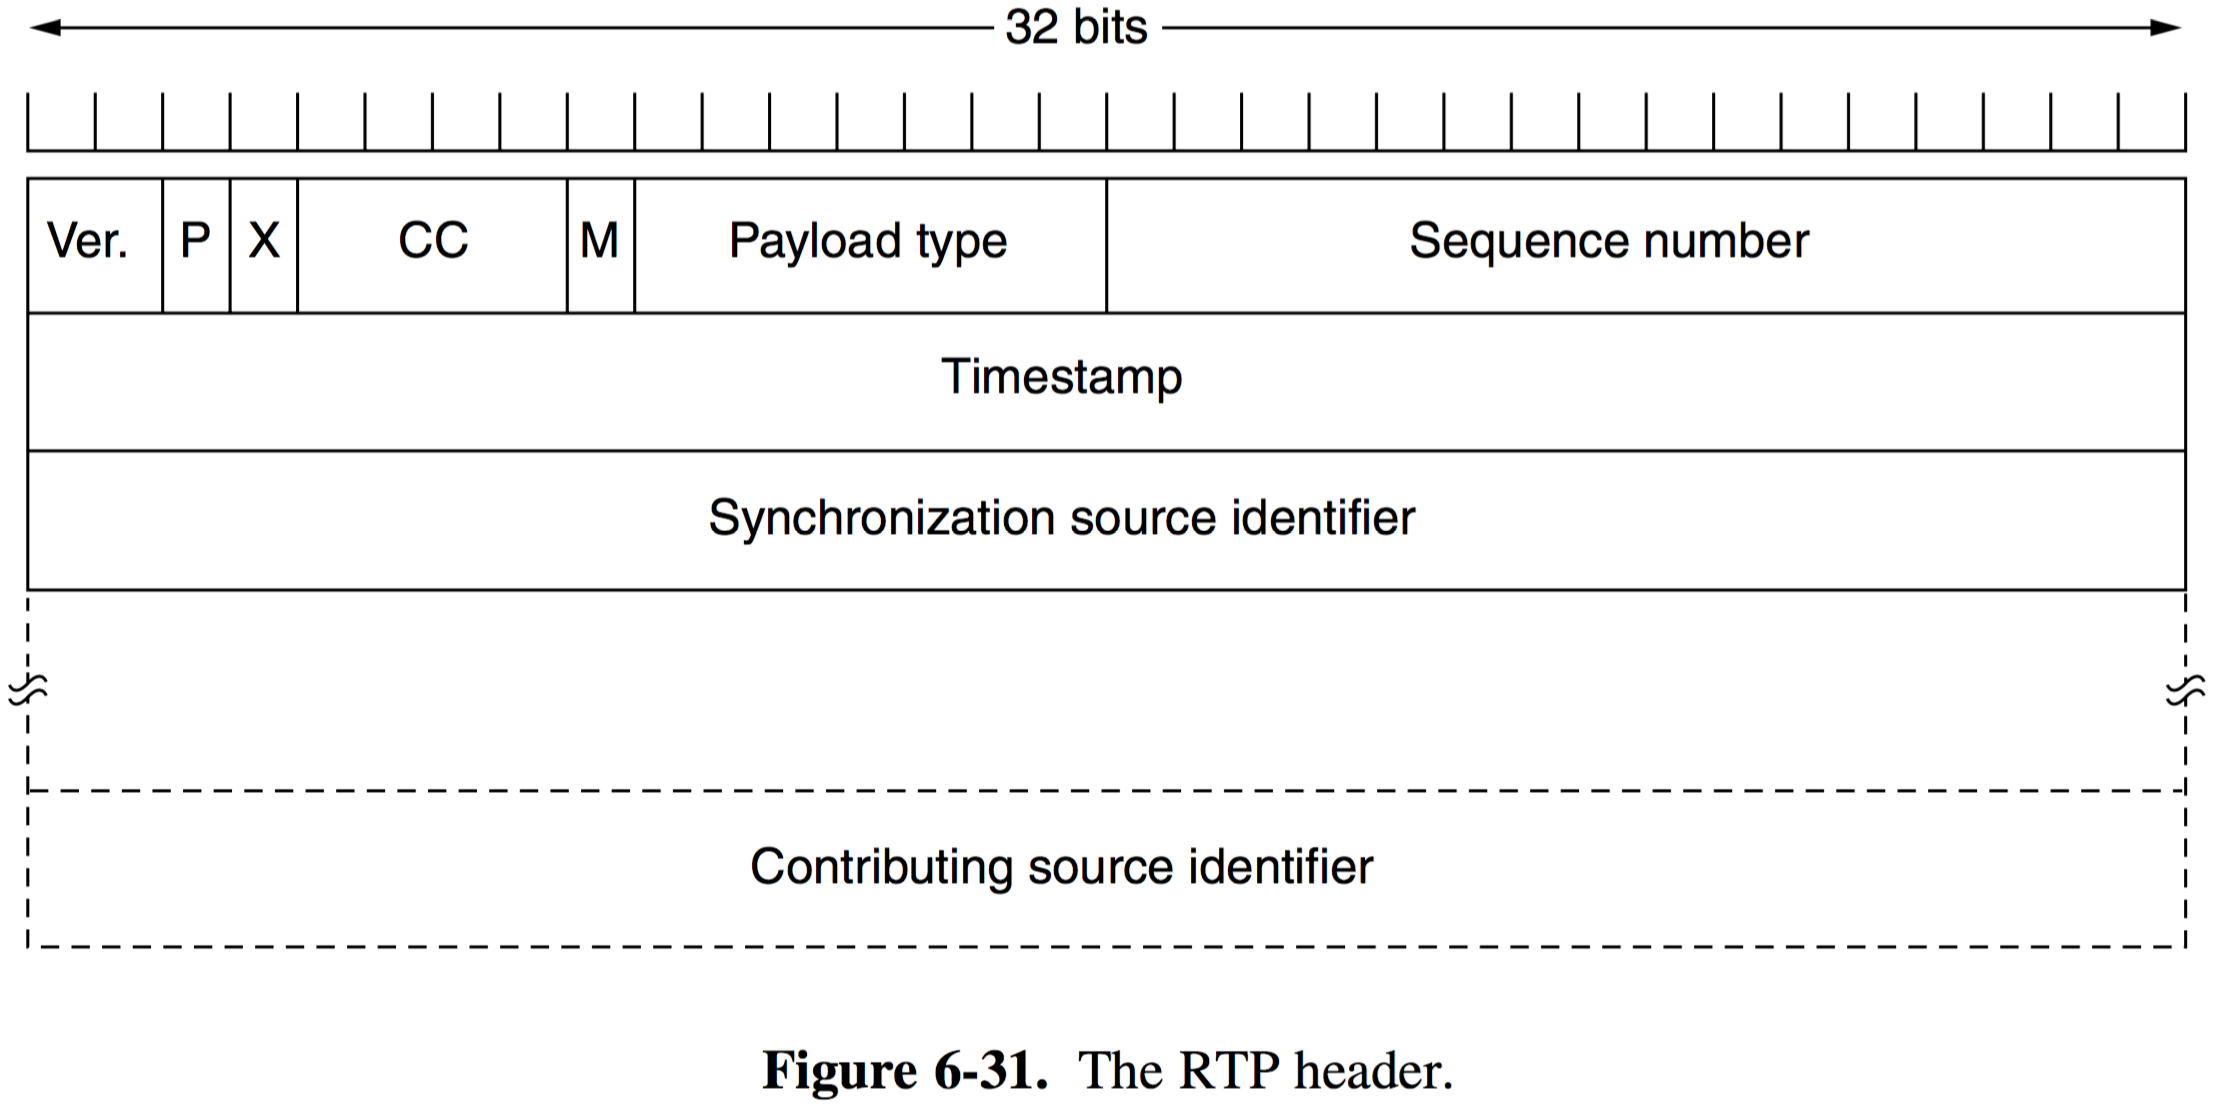
\includegraphics[width=10cm, height=6cm]{./imagenes/rt.png} 
	\end{center}

	\par El campo \textit{ CC} indica cuántas fuentes de contribución están presentes, de 0 a 15. El \textit{bit M} es un bit marcador específico de la aplicación. Puede utilizarse para marcar el inicio de una trama de video, el inicio de una palabra en un canal de audio o algo más que la aplicación entienda. El campo \textit{Tipo de carga útil} indica cuál algoritmo de codificación se utilizó (por ejemplo, audio de 8 bits sin compresión, MP3, etc.). Puesto que cada paquete lleva este campo, la codificación puede cambiar durante la transmisión. El \textit{Número de secuencia} es simplemente un contador que se incrementa con cada paquete RTP enviado. Se utiliza para detectar paquetes perdidos.
	
	\par La fuente del flujo produce la \textit{Estampa de tiempo} para indicar cuándo se creó la primera muestra en el paquete. Este valor puede ayudar a reducir la variabilidad de la sincronización conocida como \textbf{variación del retardo} (\textit{jitter}) en el receptor, al desacoplar la reproducción del tiempo de llegada del paquete. El \textit{Identicador de origen} de sincronización indica a cuál flujo pertenece el paquete. Es el método utilizado para multiplexar y desmultiplexar varios flujos de datos en un solo flujo de paquetes UDP. Por último, los \textit{Identicadores de origen de contribución}, en caso de que haya, se utilizan cuando hay mezcladoras en el estudio. En ese caso, la mezcladora es el origen de la sincronización y los flujos que se mezclan se listan aquí.

%FALTA control de congestion
\section{Los protocolos de transporte de internet: TCP}

\subsection{Introducción a TCP}
	
	\par La mayoría de las aplicaciones en internet necesitan una entrega en secuencia 
confiable, para ellos se diseñó \textbf{TCP (Transmission Control Protocol)} que sirve 
para proporcionar un flujo de bytes confiable de extremo a extremo a través de una 
interred no confiable. TCP tiene un diseño que se adapta de manera dinámica a las 
propiedades de la interred y que se sobrepone a muchos tipos de fallas.

	\par Cada máquina que soporta TCP tiene una entidad de transporte TCP (ETCP), ya 
sea un procedimiento de biblioteca, un proceso de usuario, o parte del kernel. En todos 
los casos maneja flujos TCP e interactúa con la capa IP. Una ETCP acepta flujos de 
datos de usuario de procesos locales, los divide en fragmentos que no excedan los 64 
KB, y envía cada fragmento como un datagrama IP independiente. Cuando los 
datagramas que contienen datos TCP llegan a una máquina, se pasan a la ETCP, la cual 
reconstruye los flujos de bytes originales. Usaremos la palabra TCP para referirnos: a 
veces a la ETCP y a veces al protocolo TCP.

	\par La capa IP no proporciona ninguna garantía de que los datagramas se entregarán 
de manera apropiada, por lo que corresponde a TCP terminar los temporizadores y 
retransmitir los datagramas conforme sea necesario.

	\par Los datagramas que llegan podrán hacerlo en el orden incorrecto, esto sucede 
cuando se trabaja con redes de datagramas. Corresponde a TCP reensamblarlos en 
mensajes en la secuencia apropiada ya que usualmente la capa de aplicación del 
receptor necesita procesar los mensajes en el orden en que fueron enviados.

\subsection{El modelo del servicio TCP}
	
	\par El servicio TCP se obtiene al hacer que tanto el servidor como el cliente creen 
puntos terminales llamados \textbf{\textit{sockets}}. Cada socket tiene una dirección 
que consiste en la dirección IP del host, y un número de 16 bits llamado \textbf{puerto}, el cual es local a ese host. Un puerto es el nombre TCP para un TSAP.

	\par Para obtener el servicio TCP se debe establecer de manera explícita una conexión entre el socket en la máquina emisora y uno en la máquina receptora. Un socket puede usarse para múltiples conexiones al mismo tiempo, dos o más conexiones pueden terminar en el mismo socket. Las conexiones se identifican mediante los identificadores de sockets de los dos extremos, es decir (socket1, socket2).

	\par Todas las conexiones TCP son de dúplex total y de punto a punto.
	\begin{itemize}
		\item Dúplex total: el tráfico puede ir en ambas direcciones al mismo tiempo.
		\item Punto a punto: cada conexión tiene exactamente dos puntos finales.
		\item  TCP no soporta la multidifusión ni la difusión.
	\end{itemize}

	\par Una conexión TCP es un flujo de bytes, no un flujo de mensajes. Los límites de los 
mensajes no se preservan de extremo a extremo.

	\textbf{Ejemplo:} el proceso emisor realiza 4 escrituras de 512 B en el flujo TCP, tal 
vez estos datos se entreguen al proceso receptor como 4 fragmentos de 512 B, o dos 
fragmentos de 1024 B, o uno de 2048 B o de alguna otra forma.

	\begin{center}
	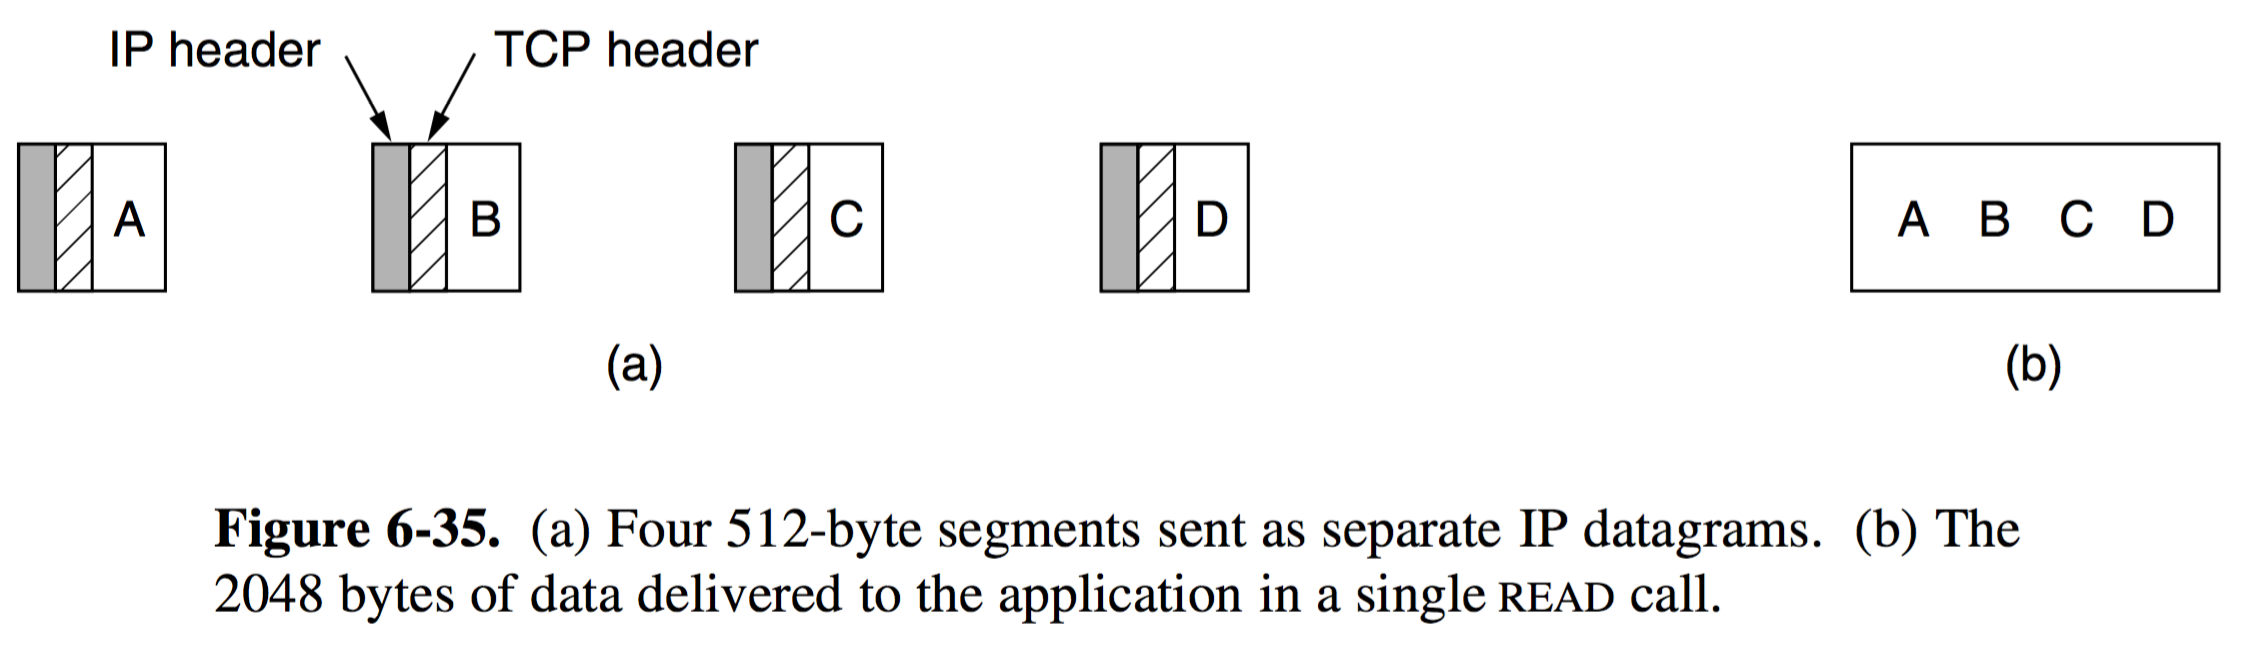
\includegraphics[width=14cm, height=4cm]{./imagenes/tcp.png} 
	\end{center}

	\par No hay manera que el receptor detecte las unidades en las que se escribieron los 
datos. El software TCP no tiene idea de lo que significan los bytes y no le interesa 
averiguarlo.

	\par Cuando una aplicación pasa datos a TCP, este decide si los envía inmediatamente 
o si los almacena en el búfer a fin de recolectar una gran cantidad y luego enviarlos al 
mismo tiempo. Sin embargo la aplicación algunas veces necesita que los datos se 
envíen de inmediato.

	\textbf{Ejemplo:} si un usuario inicia una sesión con una máquina remota. Una vez que 
se termina una línea de comandos y se introduce un retorno de carro es esencial que la 
línea se envíe a la máquina remota inmediatamente y que no se almacene en el búfer 
hasta que llegue la siguiente línea. Para obtener los datos, las aplicaciones pueden 
utilizar el indicador \textbf{PUSH} que es una señal para TCP de que no debe retrasar 
la transmisión, si llegan indicadores PUSH antes de que el primero se haya transmitido 
(por ejemplo, debido a que la línea de salida está ocupada), TCP es libre de recolectar 
todos los datos con indicadores PUSH en un solo datagrama IP, sin ninguna separación 
entre las diversas piezas.

	\par Cuando un usuario interactivo oprime las teclas \emph{Ctrl+C} o \textit{Supr} para 
interrumpir una operación remota que ha iniciado, la aplicación emisora coloca 
información de control en el flujo de datos y se la da a TCP junto con el indicador 
\textbf{URGENT}. Este evento ocasiona que TCP interrumpa el encolamiento de datos 
y transmita inmediatamente todo lo que tenga para esa conexión. Cuando el destino 
recibe los datos urgentes, se interrumpe la aplicación receptora, a fin de que pueda 
detener lo que está haciendo y que lea el flujo de datos para leer los datos urgentes.
El final de los datos urgentes se marca para que la aplicación sepa dónde terminan.
El inicio de estos no se marca; la aplicación tiene que averiguarlo.

\subsection{Direccionamiento en TCP}

	\par Los numeros de puerto menores que 1024 están reservados para los servicios 
estándar que, por lo general, sólo los usuarios privilegiados pueden iniciar. Éstos se 
llaman \textbf{puertos bien conocidos}.

	\begin{center}
	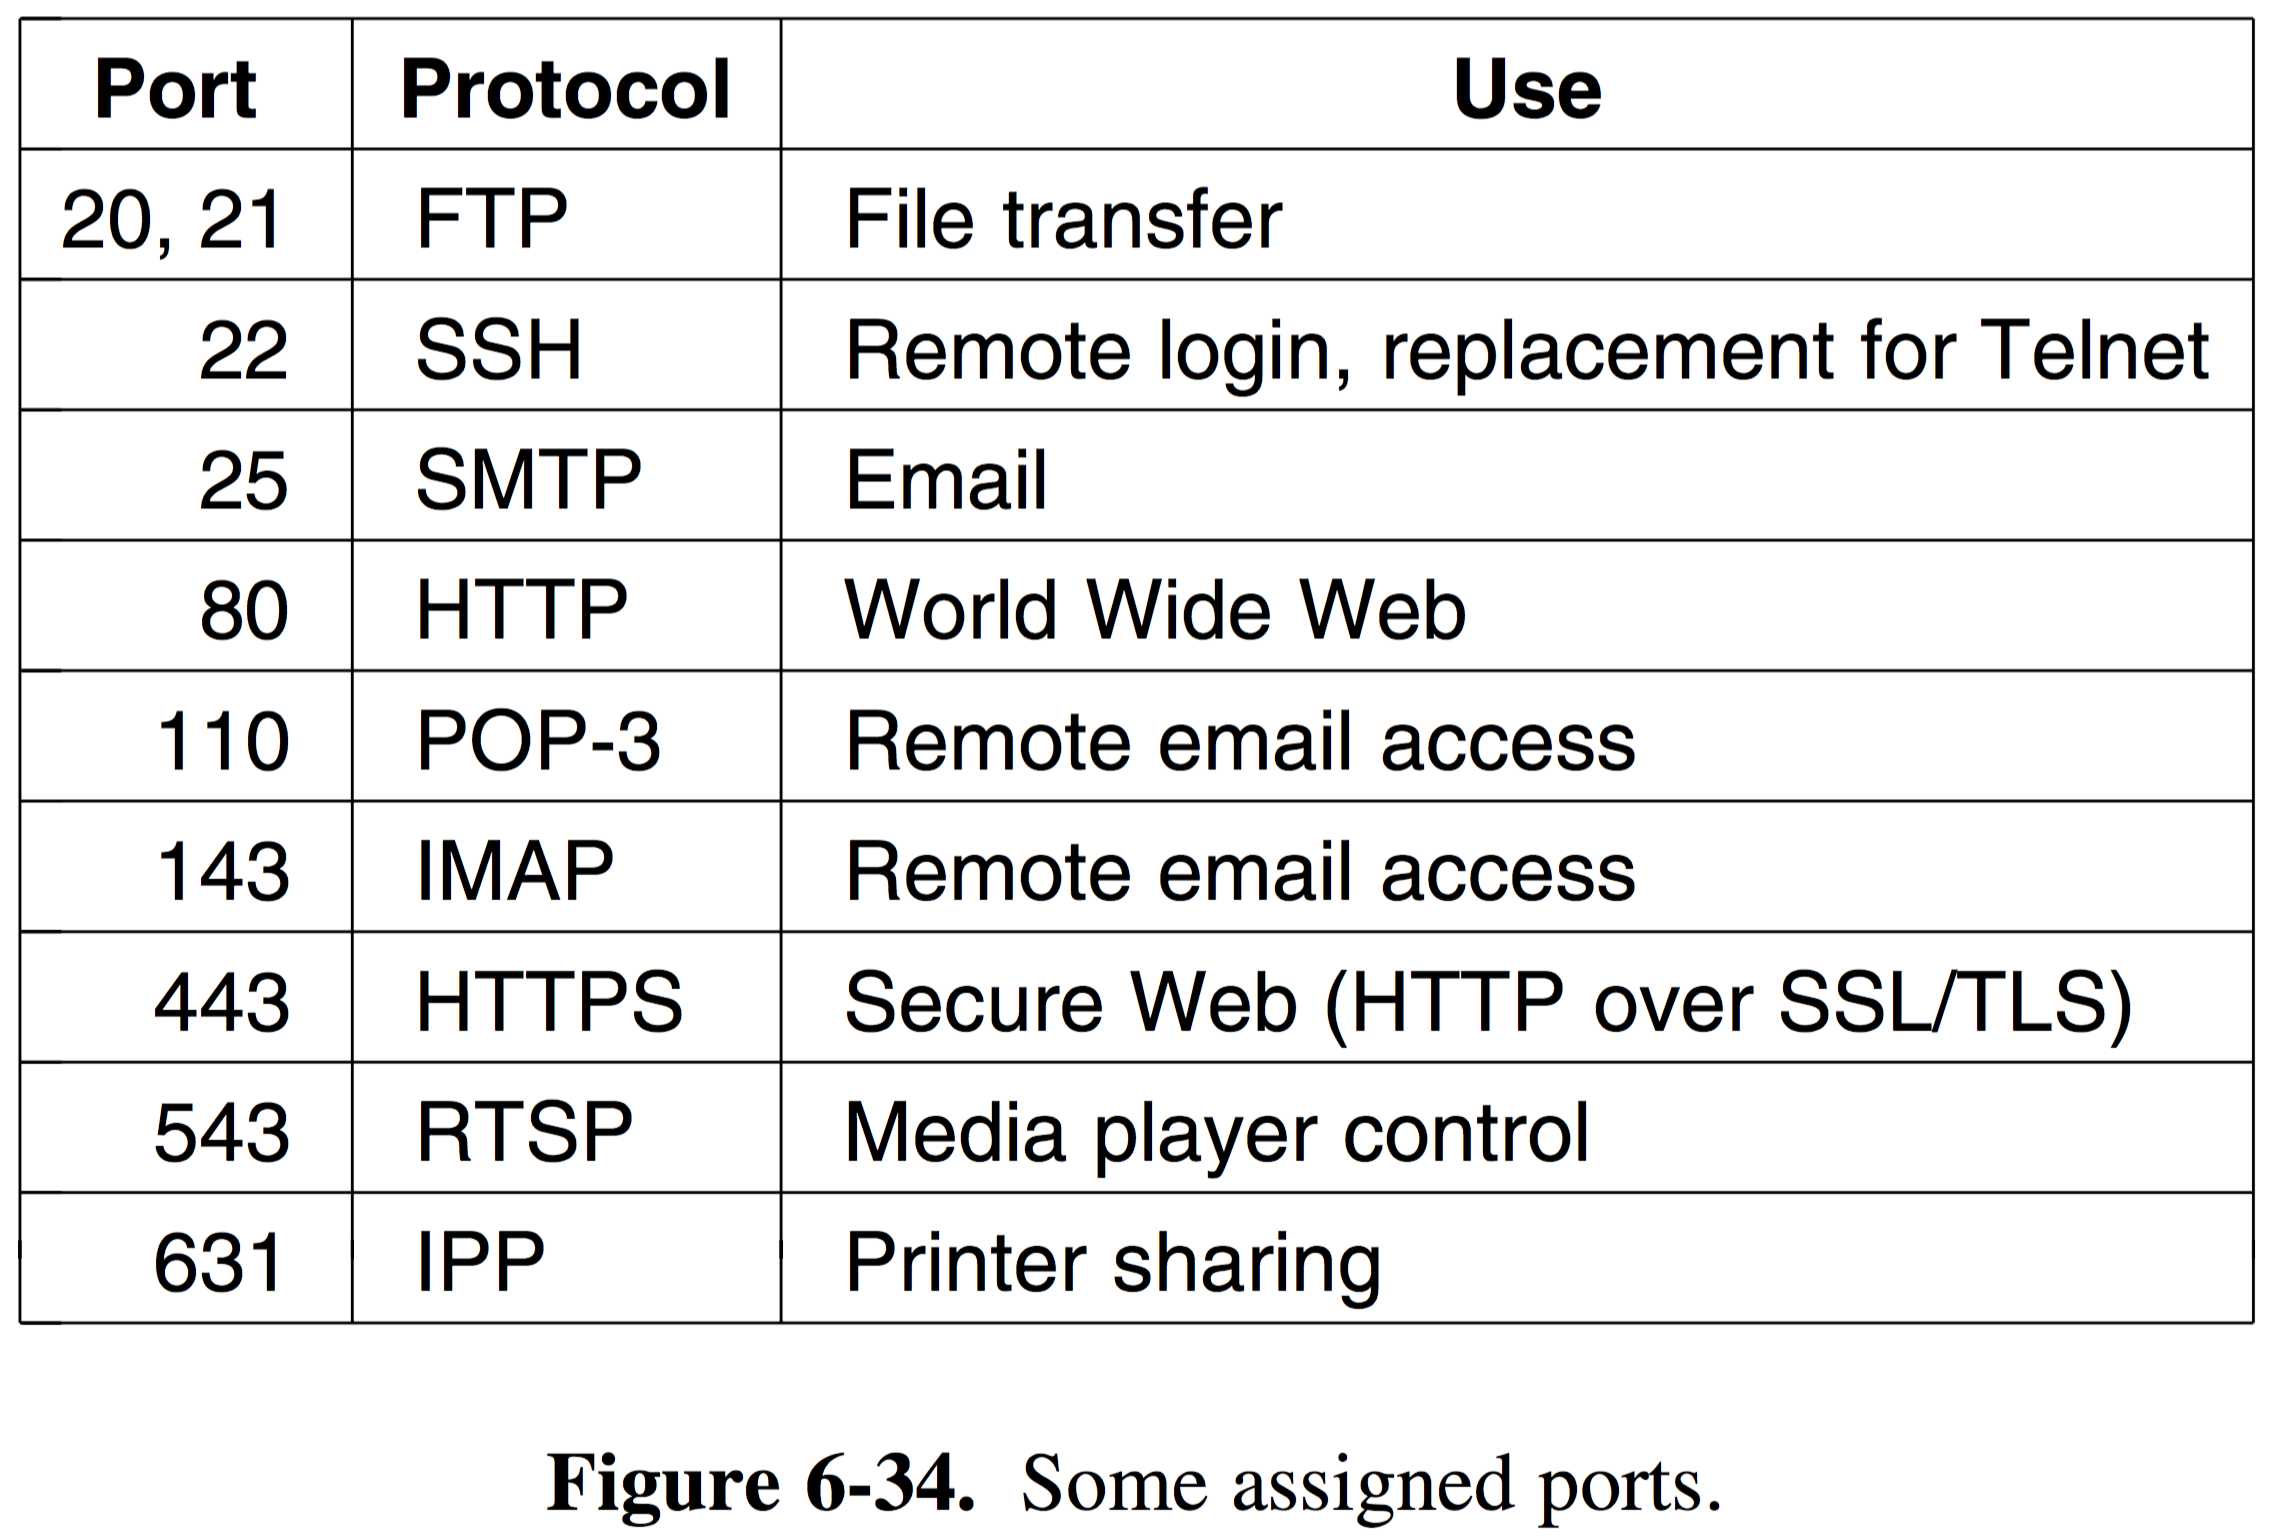
\includegraphics[width=9cm, height=6cm]{./imagenes/protocolo.png} 
	\end{center}


	\par Podría ser posible que el demonio FTP se conecte por sí solo al puerto 21 en 
tiempo de arranque, que el demonio SSH se conecte por sí solo al puerto 22 en tiempo 
de arranque, y así en lo sucesivo. Sin embargo, hacer lo anterior podría llenar la 
memoria con demonios que están inactivos la mayor parte del tiempo. En su lugar, lo 
que se hace por lo general es que un solo demonio, llamado \emph{demonio de 
Internet (inetd)}, se conecte por sí solo a múltiples puertos y espere la primera 
conexión entrante. Cuando eso ocurre, \emph{inetd} bifurca un nuevo proceso y 
ejecuta el demonio apropiado en él, para dejar que ese demonio maneje la solicitud. De 
esta forma, los demonios distintos a \textit{inetd} sólo están activos cuando hay 
trabajo para ellos. \emph{Inetd} consulta un \textbf{archivo de configuración} para 
saber cuál puerto utilizar. El administrador del sistema puede 
configurar el sistema para tener demonios permanentes en los puertos más ocupados 
e \emph{inetd} en los demás.

\subsection{El protocolo TCP}

	\par Cada byte de una conexión TCP tiene su propio número de secuencia de 32 bits. 
Los números de secuencia separados de 32 bits se usan para confirmaciones de 
recepción y para el mecanismo de ventana. La entidad TCP emisora y la receptora 
intercambian datos en forma de segmentos. Un segmento consiste en un encabezado 
TCP fijo de 20 bytes (más una parte opcional) seguido de 0 o más bytes de datos. El 
software de TCP decide el tamaño de los segmentos; puede acumular datos de varias 
escrituras para formar un segmento, o dividir los datos de una escritura en varios 
segmentos.

	\par Hay dos límites que restringen el tamaño de segmento:
		\begin{itemize}
			\item Cada segmento incluido el encabezado TCP, debe caber en la carga útil de 
		65.515 bytes del IP.
			\item Cada red tiene una unidad máxima de transferencia (MTU) y cada segmento 
		debe caber en la MTU.
			\item En la práctica la MTU es generalmente de 1500 bytes (el tamaño de la 
		carga útil de Ethernet).
		\end{itemize}	 

	\par Cuando un transmisor envía un segmento, también inicia un temporizador. Cuando 
llega el segmento a destino, la ETCP receptora devuelve un segmento (con datos si 
existen, de otro modo sin ellos) que contiene un número de confirmación de recepción 
igual al siguiente número de secuencia que espera recibir. Si el temporizador del emisor 
expira antes de la recepción de la confirmación, el emisor envía de nuevo el segmento.

\subsubsection{Problemas a manejar/resolver por TCP eficientemente:}
\begin{itemize}
	\item Pueden llegar segmentos fuera de orden, por lo que los bytes 3072-4095 
	podrían llegar pero no enviarse confirmación de recepción, porque los bytes 
	2048-3071 no han aparecido aún.
	\item También pueden retardarse segmentos en tránsito durante tanto tiempo que 
	el temporizador del emisor expira y los segmentos se retransmiten.
	\item Las retransmisiones podrían incluir rangos de bytes diferentes a los de la 
	transmisión original, lo cual requiere una administración cuidadosa para llevar el 
	control de los bytes que se han recibido correctamente en un momento 
	determinado. Esto es factible ya que cada byte del flujo tiene su propio
	desplazamiento único.
\end{itemize}

\subsection{El encabezado del segmento TCP}

	\par En la figura 6-36 se muestra la distribución de un segmento TCP. Cada segmento 
comienza con un encabezado de formato fijo de 20 bytes. El encabezado fijo puede ir 
seguido de encabezado de opciones. Después de las opciones, si las hay, pueden 
continuar hasta 65535$-$20$-$20$=$65495 bytes de datos, donde los primeros 20 se 
refieren al encabezado IP y los segundos al encabezado TCP. Los segmentos sin datos 
son legales y se usan por lo común para confirmaciones de recepción y mensajes de 
control.

	\begin{center}
		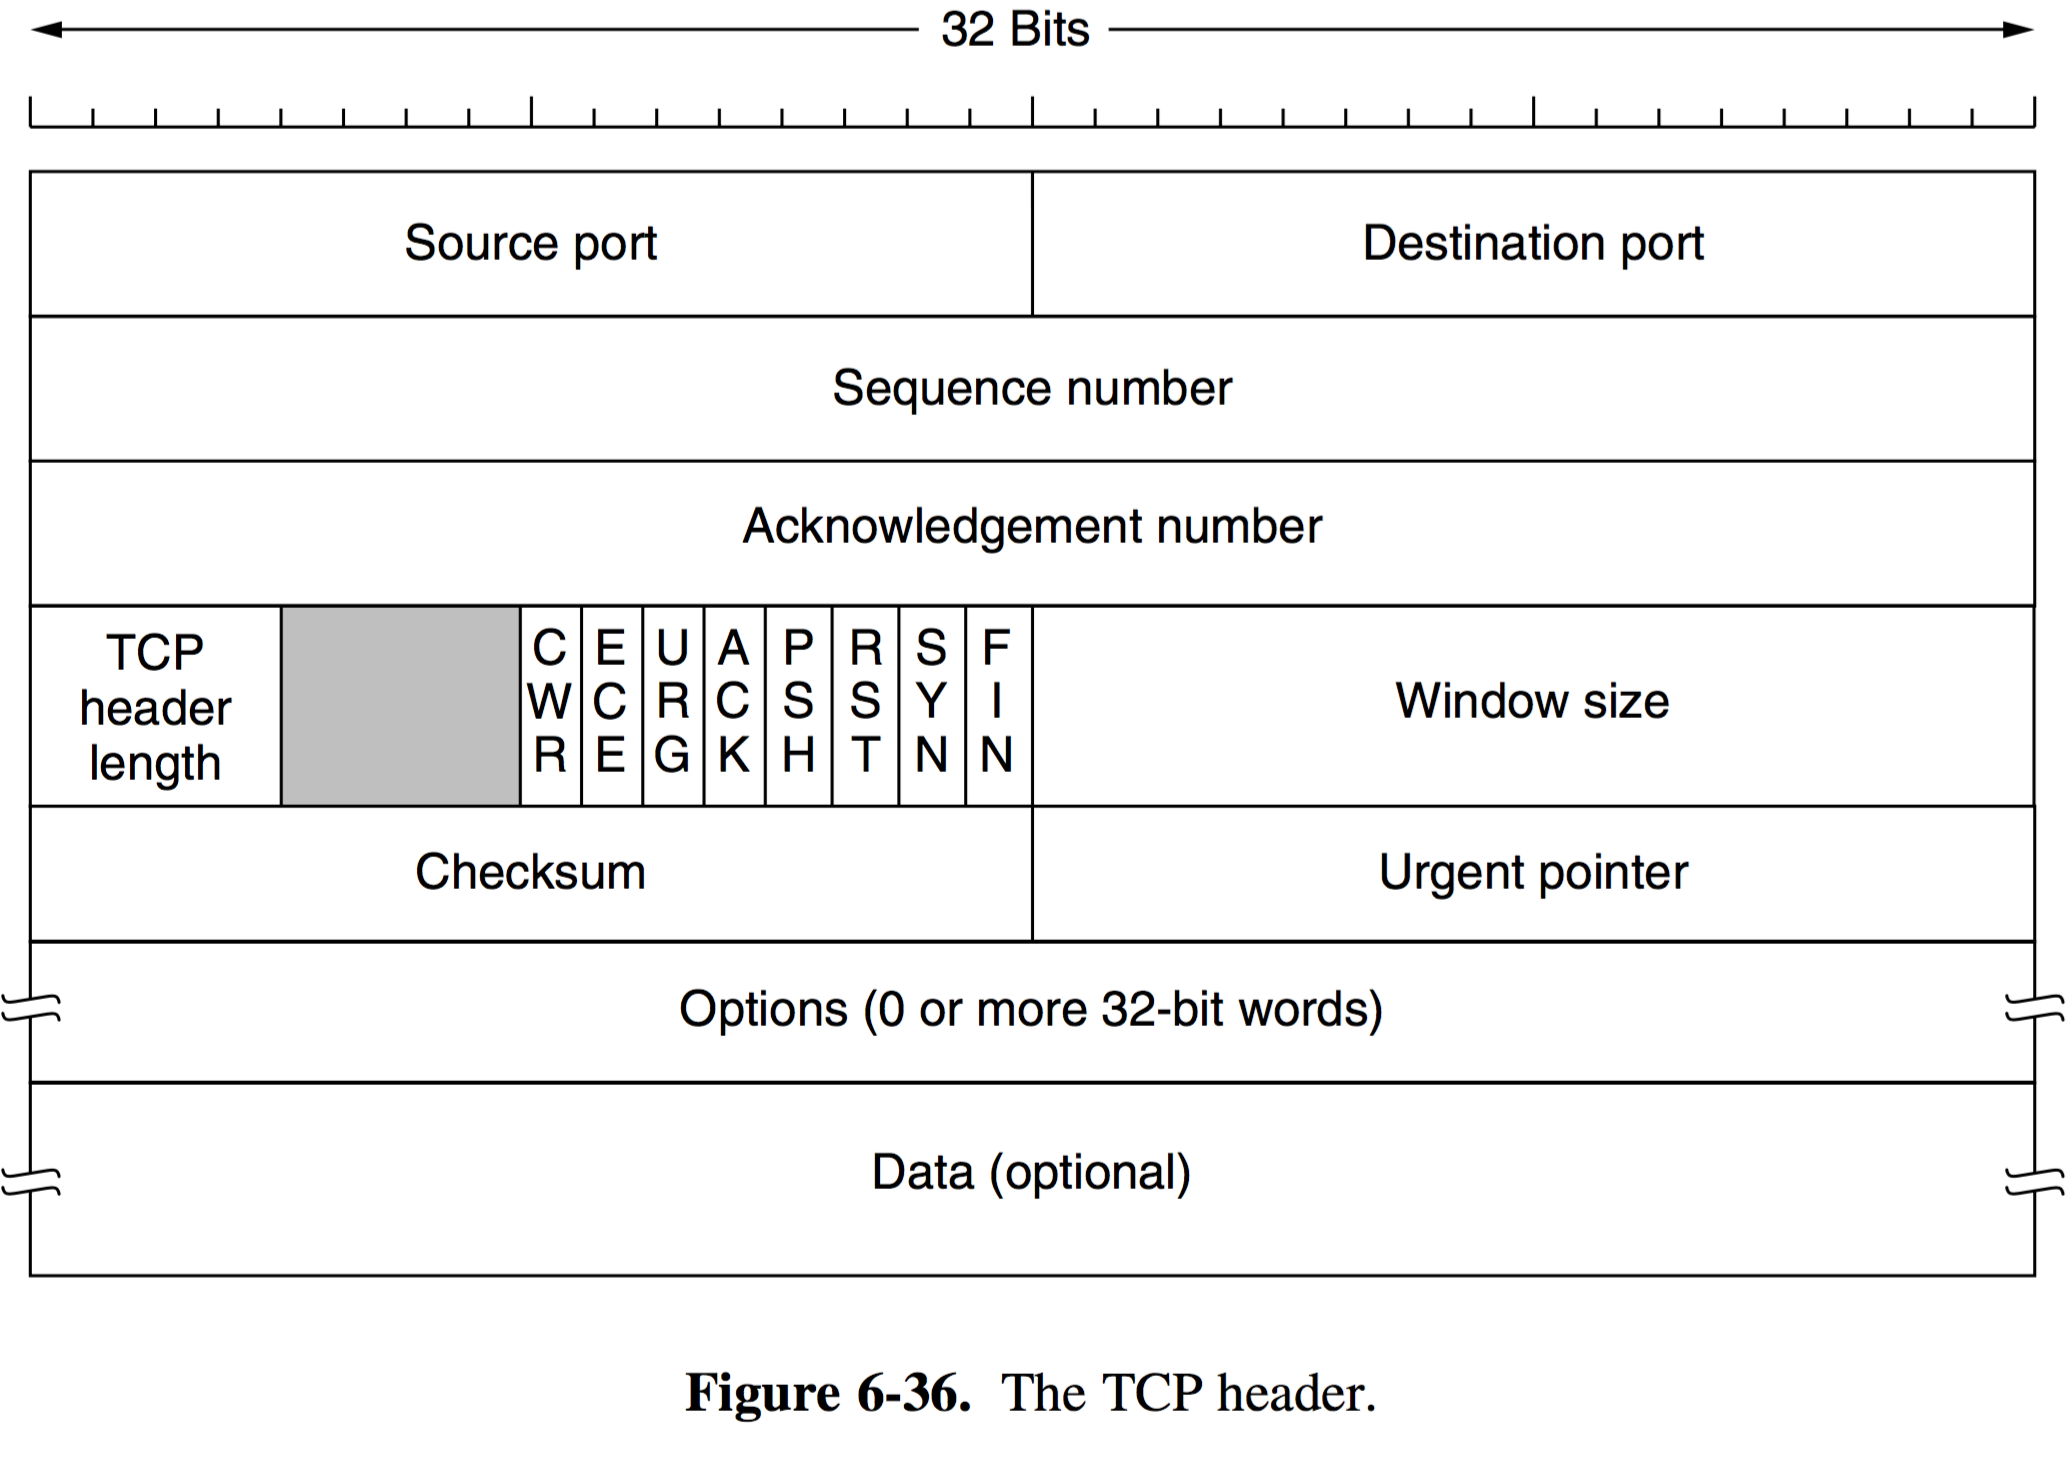
\includegraphics[width=9cm, height=6cm]{./imagenes/encabezado.png} 
	\end{center}

	\par Los campos de \textit{puerto de origen} y \textit{puerto de destino} identifican 
los puntos terminales locales de la conexión. La dirección de un puerto más la dirección 
IP del host forman un punto terminal único de 48 bits. Los puntos terminales de origen 
y de destino en conjunto identifican la conexión.

	\par Los campos \textit{número de secuencia} y \textit{número de confirmación de 
recepción} desempeñan sus funciones normales. El segundo indica el siguiente byte 
esperado, no el último byte correctamente recibido. Ambos tienen 32 bits de longitud porque cada byte de datos está numerado en el flujo TCP.

	\par La \textit{longitud del encabezado TCP} indica la cantidad de palabras de 32 
bits contenidas en el encabezado TCP. Esta información es necesaria porque el campo 
\textit{Opciones} es de longitud variable, por lo que el encabezado también. Este 
campo indica el comienzo de los datos en el segmento, medido en palabras de 32 bits, 
pero ese número es simplemente la longitud del encabezado en palabras. A 
continuación viene un campo de 6 bits que no se usa.

	\par Luego vienen 8 indicadores de 1 bit:
		\begin{itemize}
			\item \textbf{CWR} y \textbf{ECE} se utilizan para indicar congestión cuando se 
		usa ECN (Notificación Explícita de Congestión). ECE se establece para indicar una 
		\textit{ECN-Echo} a un emisor TCP y decirle que reduzca su velocidad cuando el 
		receptor TCP recibe una indicación de congestión de la red. CWR se establece 
		para indicar una \textit{Ventana de congestión} reducida del emisor TCP al 
		receptor TCP, de modo que sepa que el emisor redujo su velocidad y puede dejar 
		de enviar la \textit{Repetición de ECN}.
			\item \textbf{URG} se establece en 1 si está en uso el \textit{Apuntador Urgente}, el cual 
		sirve para indicar un desplazamiento en bytes a partir del número actual de 
		secuencia en el que se encuentran datos urgentes, sustituye los mensajes de 
		interrupción y un mecanismo rudimentario para permitir que el emisor envíe una 
		señal al receptor sin implicar al TCP en la razón de la interrupción.
			\item \textbf{ACK} se establece en 1 para indicar que el \textit{Número de confirmación 
		de recepción} es válido. Si es 0, el segmento no contiene una confirmación de 
		recepción, por lo que se ignora el campo de número de confirmación de 
		recepción.
			\item \textbf{PSH} indica datos que se deben transmitir de inmediato. Por este medio se 
		solicita atentamente al receptor que entregue los datos a la aplicación a su 
		llegada y no los almacene en búfer hasta la recepción de un búfer completo.
			\item \textbf{RST} se usa para restablecer de manera repentina una conexión 
		que se ha confundido debido a una falla de host o alguna otra razón. También se 
		usa para rechazar un segmento no válido o un intento de abrir una conexión. Por 
		lo general, si usted recibe un segmento con el bit RST encendido, tiene un 
		problema entre manos.
			\item \textbf{SYN} se usa para establecer conexiones, es decir, denotar 
		\textit{CONNECTION REQUEST} y \textit{CONNECTION ACCEPTED}.
			\item \textbf{FIN} se usa para liberar una conexión y especifica que el emisor no 
		tiene más datos que \textit{transmitir}. 
		\end{itemize}

	\par El control de flujo en TCP se maneja mediante una ventana deslizante de tamaño 
variable. El campo \textit{Tamaño de ventana} indica la cantidad de bytes que se 
pueden enviar, comenzando por el byte cuya recepción se ha confirmado. Un campo 
de \textit{Tamaño de ventana} de 0 es válido e indica que se han recibido los bytes 
hasta \textit{Número de confrmación de recepción}$-$1.

\subsection{Establecimiento de una conexión TCP}

	\par En TCP las conexiones se establecen mediante el acuerdo de tres vías. Para establecer una conexión, el \textbf{servidor} espera en forma pasiva una conexión entrante mediante la ejecución de las primitivas LISTEN y ACCEPT en ese orden, ya sea que se especifique un origen determinado o a nadie en particular.

	\par Del otro lado el cliente ejecuta una primitiva CONNECT en la que especifica la dirección y el puerto con el que se desea conectar, el tamaño máximo de segmento TCP que está dispuesto a aceptar y de manera opcional algunos datos de usuario (por ejemplo, una contraseña). La primitiva CONNECT envía un segmento TCP con el bit SYN encendido y el bit ACK apagado, y espera una respuesta.

	\par Cuando este segmento llega al destino, la entidad TCP de ahí revisa si hay un proceso que haya ejecutado una primitiva LISTEN en el puerto que se indica en el campo \textit{Puerto de destino}. Si no lo hay, envía una respuesta con el bit RST encendido para rechazar la conexión.

	\par Si algún proceso está escuchando en el puerto, ese proceso recibe el segmento TCP entrante y puede entonces aceptar o rechazar la conexión. Si la acepta, se devuelve un segmento de confirmación de recepción. La secuencia de segmentos TCP enviados en el caso normal se muestra en la figura 6-37(a). Observe que un segmento SYN consume 1 byte de espacio de secuencia, por lo que se puede reconocer sin ambigüedades.

	\begin{center}
		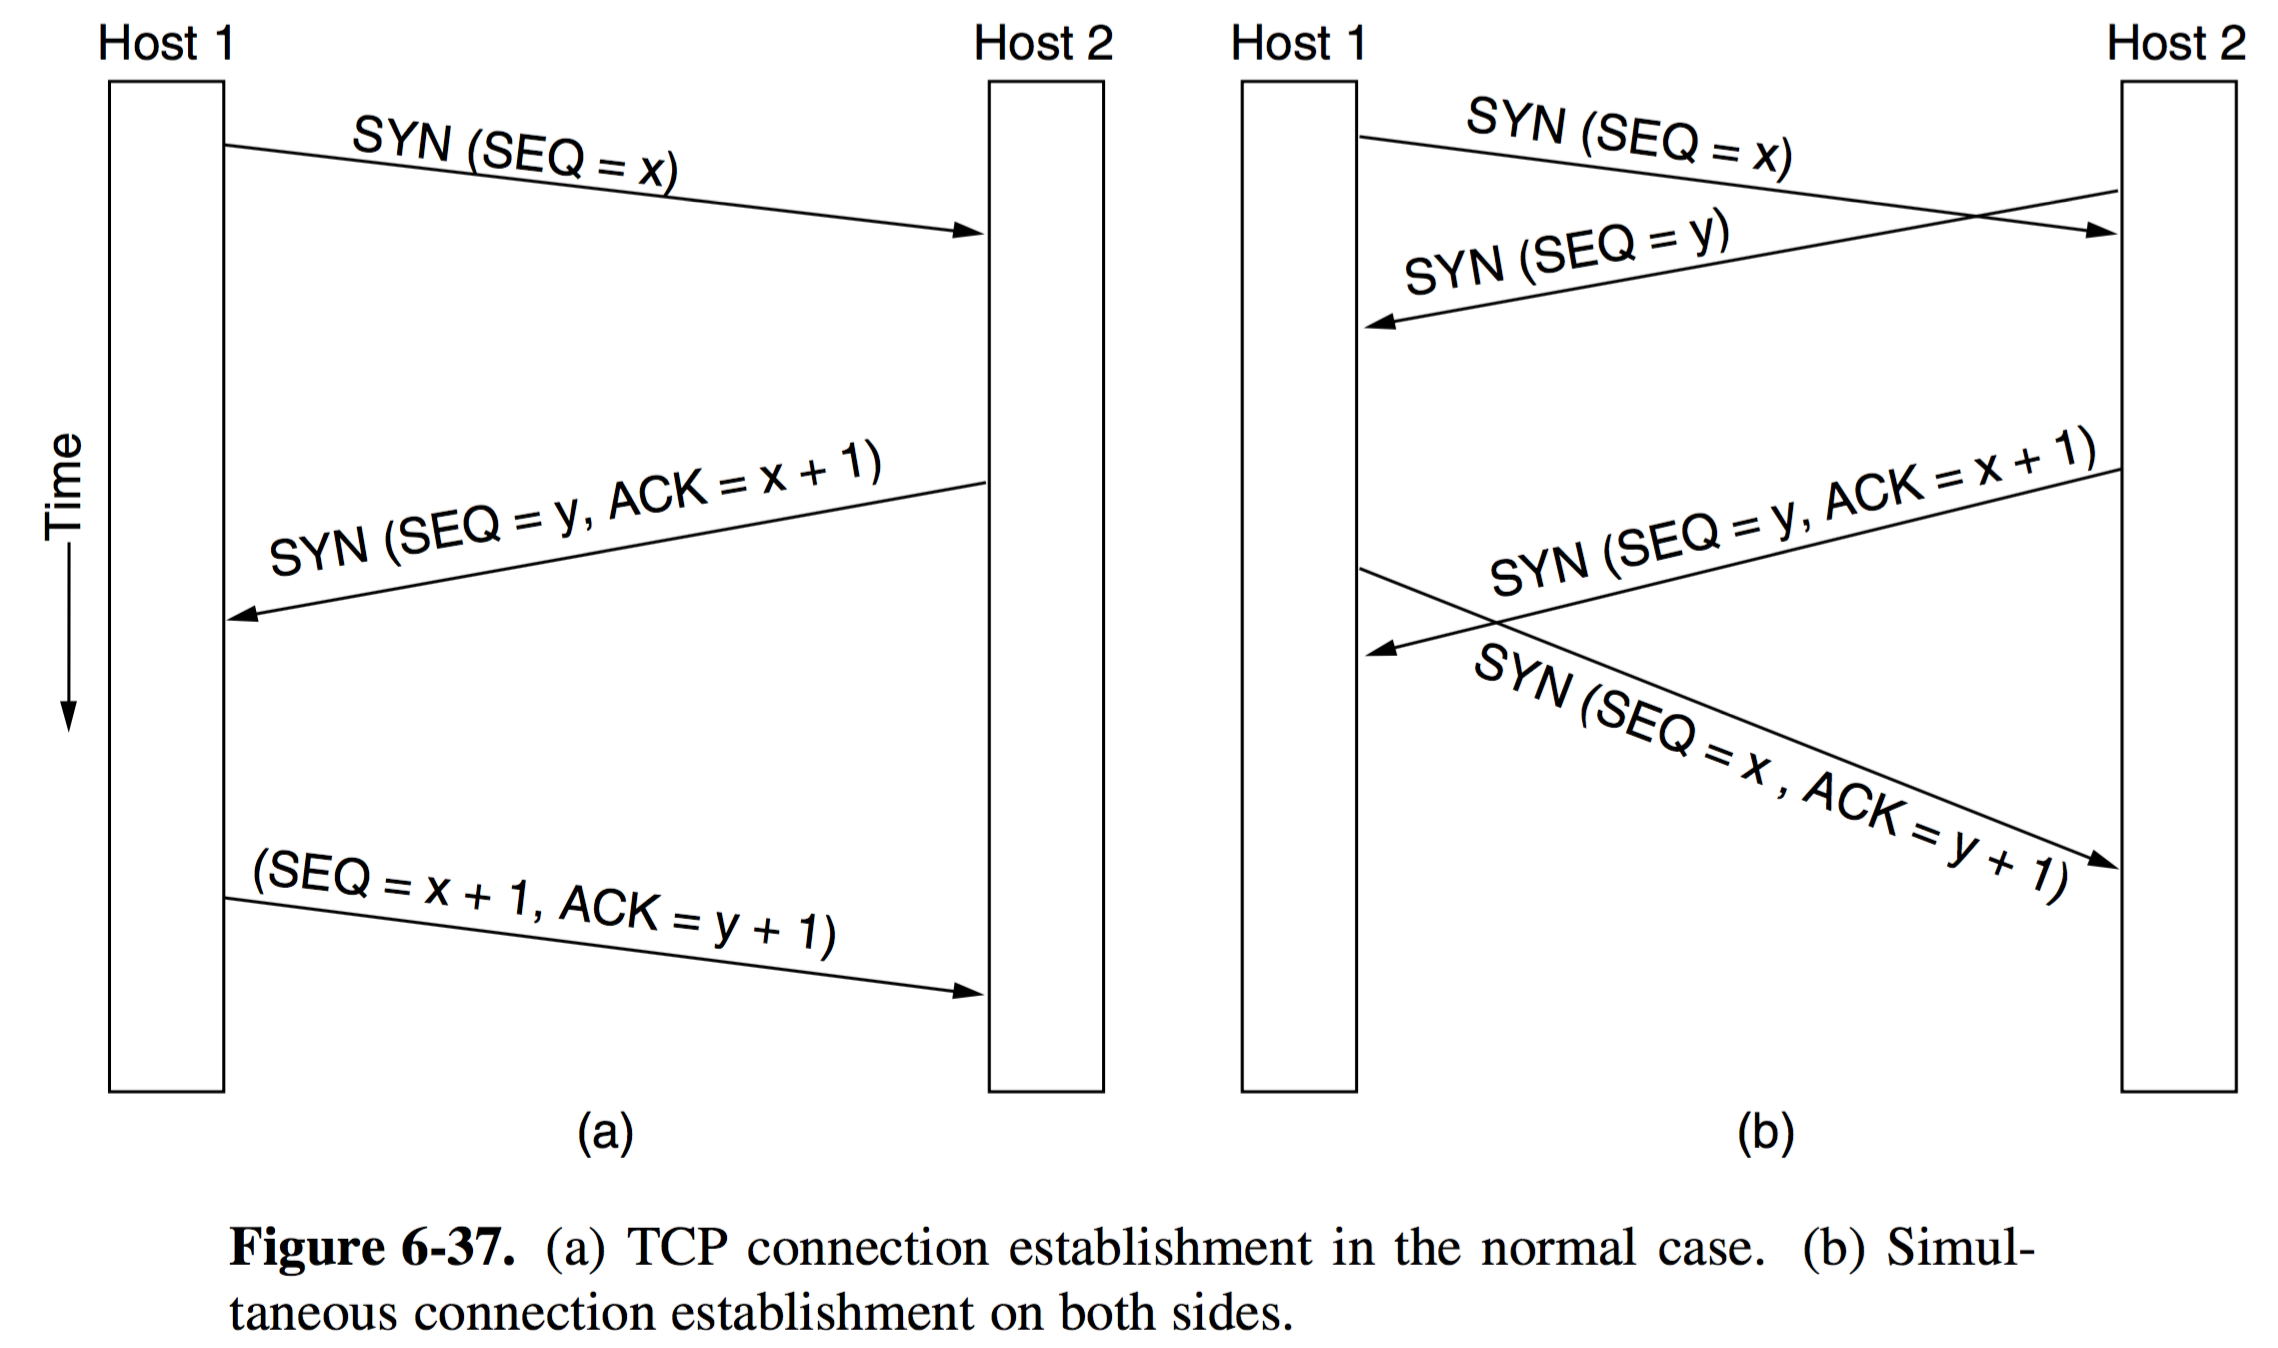
\includegraphics[width=8cm, height=6cm]{./imagenes/conexiontcp.png}
	\end{center}

\subsection{Liberación de una conexión TCP}

	\par Aunque las conexiones TCP son full dúplex, para entender la manera en que se liberan las conexiones es mejor visualizarlas como un par de conexiones simplex. Cada conexión simplex se libera de manera independiente de su igual. Para liberar una conexión, cualquiera de las partes puede enviar un segmento TCP con el bit FIN establecido, lo que significa que no tiene más datos por transmitir. Al confirmarse la recepción de FIN, se apaga ese sentido para que no se transmitan nuevos datos. Sin embargo, lo datos pueden seguir fluyendo de manera indefinida por el otro sentido. Cuando se apagan ambos sentidos, se libera la conexión. Por lo general se requieren cuatro segmentos TCP para liberar una conexión: un FIN y un ACK para cada sentido. Sin embargo, es posible que el primer ACK y el segundo FIN estén contenidos en el mismo segmento, con lo cual se reduce la cuenta total a tres.
	
	\par Ambos extremos de una conexión TCP pueden enviar segmentos FIN al mismo tiempo. La recepción de ambos se confirma de la manera usual, y se apaga la conexión. De hecho, en esencia no hay diferencia entre la liberación secuencial o simultánea por parte de los hosts.
	
	\par Para evitar el problema de los dos ejércitos, se usan temporizadores. Si no llega una respuesta a un FIN en un máximo de dos tiempos de vida del paquete, el emisor del FIN libera la conexión. Tarde o temprano el otro lado notará que, al parecer, ya nadie lo está escuchando, y también expirará su temporizador. En la práctica, pocas veces ocurren problemas.
	
\subsection{Ventana deslizante de TCP}

\subsubsection{Control de flujo en TCP}
	
	\par El campo \textbf{tamaño de ventana} en el encabezado TCP indica la cantidad de bytes que pueden enviarse comenzando por el byte cuya recepción se ha confirmado. Un campo de tamaño de ventana 0 indica que se han recibido los bytes hasta número de confirmación de recepción – 1, inclusive, pero que el receptor actualmente necesita un descanso y quisiera no recibir más datos por el momento. El permiso para enviar puede otorgarse después enviando un segmento con el mismo número de confirmación de recepción y un campo tamaño de ventana distinto de 0. Si la ventana anunciada por el receptor es de 0, el emisor debe detenerse hasta que el proceso de aplicación del \textit{host receptor} retire algunos datos del búfer en cuyo momento el TCP puede anunciar una ventana más grande.

	\par Suponga que el receptor tiene un búfer de 4096 bytes, como se muestra en la figura 6-40. Si el emisor transmite un segmento de 2048 bytes que se recibe correctamente, el receptor enviará la confirmación de recepcioón del segmento. Sin embargo, dado que ahora sólo tiene 2048 bytes de espacio de búfer (hasta que la aplicación retire algunos datos de éste), anunciará una ventana de 2048 comenzando con el siguiente byte esperado.
	
	\begin{center}
		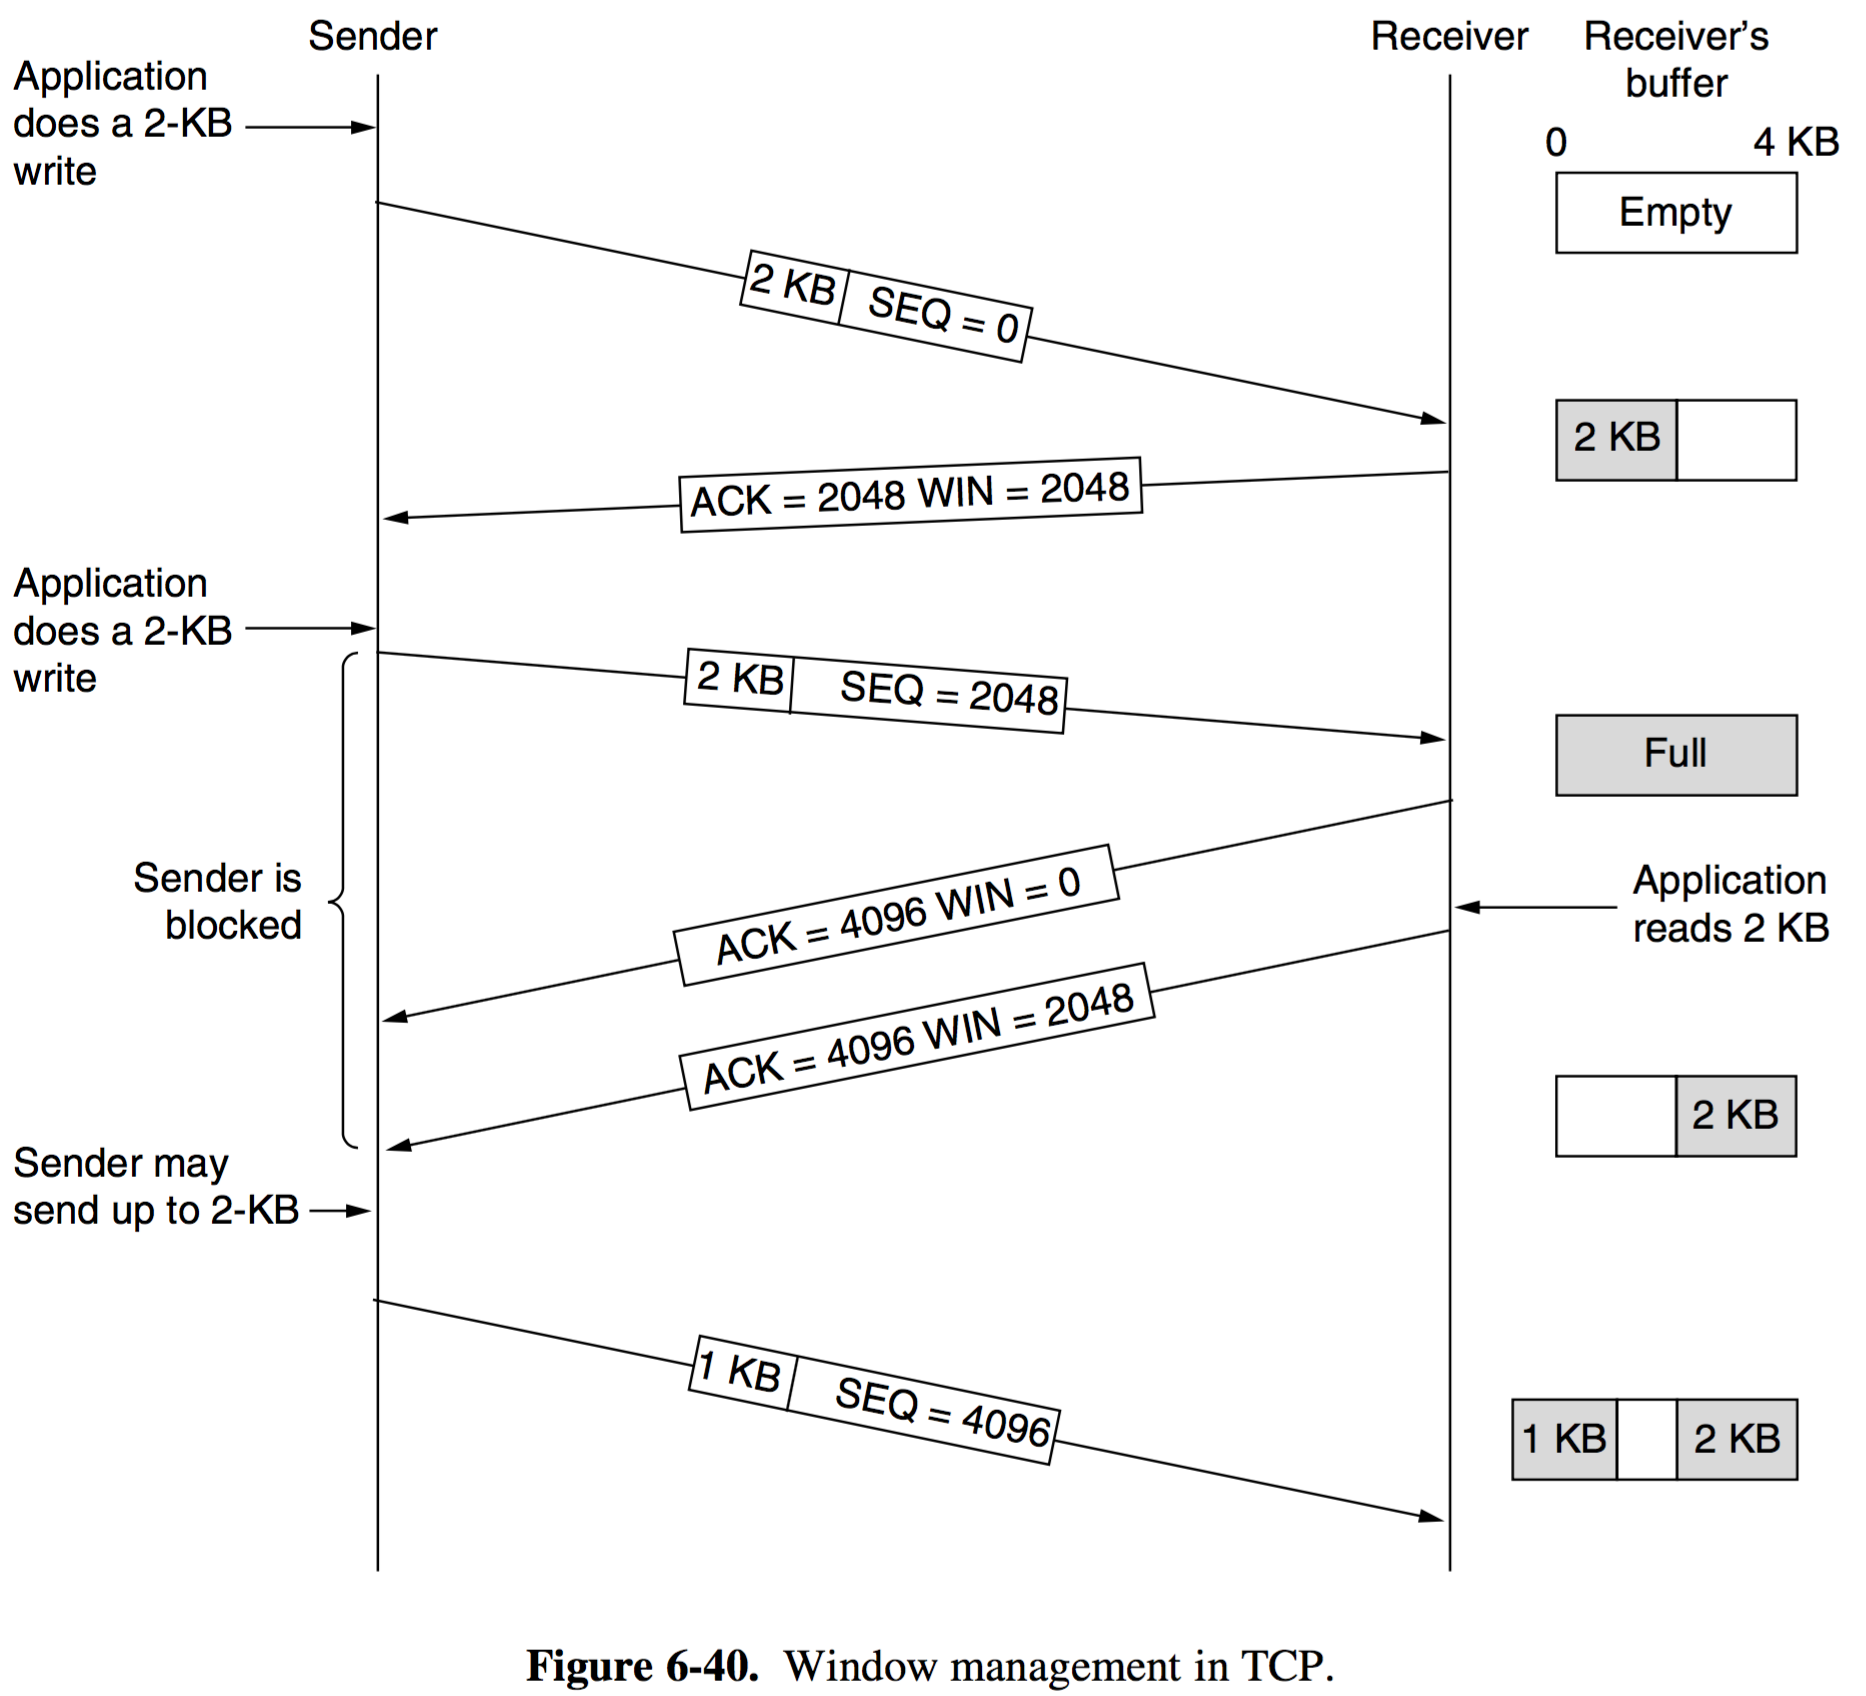
\includegraphics[width=8cm, height=6cm]{./imagenes/flujotcp.png} 
	\end{center}
	
	\par Ahora el emisor envía otros 2048 bytes, para los cuales el receptor envía la confirmación de recepción, pero la ventana anunciada tiene un tamaño de 0. El emisor debe detenerse hasta que el proceso de aplicación en el \textit{host receptor} retire algunos datos del búfer, momento en el que TCP podrá anunciar una ventana más grande y se podrán enviar más datos.

	\par Cuando la ventana es de 0, el emisor por lo general no puede enviar segmentos, salvo en dos situaciones. En primer lugar, se pueden enviar \textbf{datos urgentes} (por ejemplo, para permitir que el usuario elimine el proceso en ejecución en la máquina remota). En segundo lugar, el emisor puede enviar un segmento de 1 byte para hacer que el receptor vuelva a anunciar el siguiente byte esperado y el tamaño de la ventana. TCP proporciona explícitamente esta opción para evitar un interbloqueo si llega a perderse una actualización de ventana.

	\par No se requiere que los emisores transmitan datos tan pronto como llegan de la aplicación. Tampoco se requiere que los receptores envíen confirmaciones de recepción tan pronto como sea posible, ni que los receptores entreguen datos a la aplicación apenas los reciben. Por ejemplo, en la figura 6-40 cuando llegaron los primeros 2 KB de datos, TCP, a sabiendas que tenía disponible una ventana de 4 KB, hubiera actuado perfectamente bien si sólo almacenara en el búfer los datos hasta que llegaran otros 2 KB para transmitir un segmento con una carga útil de 4 KB. Podemos explotar esta libertad para mejorar el desempeño.
	
	\par Las confirmaciones de recepción se pueden enviar sólo después de haber recibido todos los datos hasta el byte confirmado. A esto se le conoce como \textbf{confirmación de recepción acumulativa}. Si el receptor recibe los segmentos 0, 1, 2, 4, 5, 6 y 7, puede enviar una confirmación de recepción de todos los bytes hasta el último byte del segmento 2, inclusive. Al expirar el temporizador del emisor, éste retransmitirá el segmento 3. Como el receptor ha puesto en el búfer los segmentos 4 a 7, al recibir el segmento 3 puede enviar una confirmación de recepción de todos los bytes hasta el final del segmento 7.	

	\par El campo \textit{opciones} ofrece una forma de agregar características extra no cubiertas por el encabezado normal. La opción más importante es la que permite que cada \textit{host} especifique la carga útil TCP máxima que está dispuesto a aceptar. El uso de segmentos grandes es más eficiente que el de segmentos pequeños: el encabezado de 20 bytes puede amortizarse entre más datos. Durante el establecimiento de la conexión, cada lado puede anunciar su máximo y ver el de su compañero. Si un \textit{host} no usa esta opción, tiene una carga útil predeterminada de 536 bytes. Se requiere que todos los \textit{hosts} de internet acepten segmentos TCP de $ 536 + 20 = 556  bytes $. No es necesario que el tamaño de segmento en ambas direcciones sea el mismo.

	\par En las líneas con alto ancho de banda, alto retardo o ambas cosas, la ventana de 64 KB con frecuencia es un problema. En una línea T3 (44.736 Mbps) se requieren solo 12 \textit{mseg} para enviar una ventana completa de 64 KB. Si el retardo de propagación de ida y vuelta es de 50 \textit{mseg} (típico de una fibra transcontinental), el emisor estará inactivo $3/4$ del tiempo en espera de confirmaciones de recepción.

	\par Un tamaño de ventana más grande permitirá al emisor continuar enviando datos, pero como el campo de tamaño de ventana es de 16 bits, es imposible expresar tal tamaño. La solción es usar la opción de escala de ventana, para permitir al emisor y al receptor negociar un factor de escala de ventana. Este número da la posibilidad de que ambos lados desplacen el tamaño del campo de ventana hasta 14 bits a la izquierda, permitiendo por tanto ventanas de hasta $2^{30}$ bytes. La mayoría de las implementaciones actuales de TCP manejan esta opción.

	\par Si el receptor recibe un segmento malo y luego una gran cantidad de segmentos buenos, el temporizador del protocolo TCP normal expirará en algún momento y se retransmitirán todos los segmentos sin confirmación de recepción, incluidos los que se recibieron correctamente. Se deben utilizar NAKs, para permitir que el receptor solicite un segmento/s específico/s. Tras recibirlo, puede enviar una confirmación de recepción de todos los datos que tiene en búfer, reduciendo de esta manera la cantidad de datos retransmitidos.

\subsubsection{Política de Transmisión en TCP}

	\par Considere una conexión a una terminal remota; por ejemplo, mediante el uso de SSH o telnet, que reacciona con cada pulso de tecla. En el peor de los casos, al llegar un carácter a la entidad TCP emisora, TCP crea un segmento TCP de 21 bytes que entrega al IP para que lo envíe como datagrama IP de 41 bytes. Del lado receptor, TCP envía de inmediato una confirmación de recepción de 40 bytes (20 bytes de encabezado TCP y 20 bytes de encabezado IP). Después, cuando la terminal remota lee el byte, TCP envía una actualización de ventana y recorre la ventana 1 byte hacia la derecha. Este paquete también es de 40 bytes. Por último, cuando la terminal remota procesa el carácter, lo retransmite para que se despliegue en forma local mediante un paquete de 41 bytes. En conjunto se usan 162 bytes de ancho de banda y se envían cuatro segmentos por cada carácter pulsado. Cuando el ancho de banda escasea, no es deseable este método de operación.
	
	\par Un enfoque que usa muchas implementaciones de TCP para optimizar esta situación es el de las confirmaciones de recepción con retardo. La idea es retrasar las confirmaciones de recepción y las actualizaciones de ventana por hasta 500 \textit{mseg}, con la esperanza de que lleguen algunos datos con los cuales se pueda viajar de manera gratuita. Suponiendo que la terminal hace eco en un lapso de 500 \textit{mseg}, ahora el lado remoto sólo necesita enviar de vuelta un paquete de 41 bytes, con lo cual se recorta a la mitad la cuenta de paquetes y el uso de ancho de banda.
	
	\par Aunque las confirmaciones de recepción con retardo reducen la carga impuesta en la red por el receptor, un emisor que envía varios paquetes cortos (por ejemplo, paquetes de 41 bytes que contengan 1 byte de datos) aún opera de manera ineficiente. El \textbf{algoritmo de Nagle} es una manera de reducir este uso. Lo que sugirió Nagle es sencillo: cuando llegan datos en pequeñas piezas al emisor, sólo se envía la primera pieza y el resto se almacena en búfer hasta que se confirma la recepción del byte pendiente. Después se envían todos los datos del búfer en un segmento TCP y nuevamente comienzan a almacenarse en búfer los datos hasta que se haya confirmado la recepción del siguiente segmento. Esto significa que sólo puede haber un paquete corto pendiente en cualquier momento dado. Si la aplicación envía muchas piezas de datos en el tiempo de ida y vuelta, el algoritmo de Nagle colocará todas las diversas piezas en un segmento, con lo cual se reducirá de manera considerable el ancho de banda utilizado. Además, el algoritmo establece que se debe enviar un nuevo segmento si se acumularon suficientes datos como para llenar un segmento máximo.
	
	\par Si el usuario escribe con rapidez y la red es lenta, puede entrar una cantidad importante de caracteres en cada segmento, reduciendo en gran medida el ancho de banda usado. A veces conviene inhabilitar el algoritmo de Nagle. En particular al operar una aplicación X-Windows a través de Internet, los movimientos del ratón tienen que enviarse a la computadora remota (X-Windows es el sistema de ventanas usado por la mayoría de los sistemas UNIX). Su acumulación para enviarlos en ráfagas hace que el movimiento del cursor sea errático, lo que no complace mucho a los usuarios.
	
	\begin{center}
		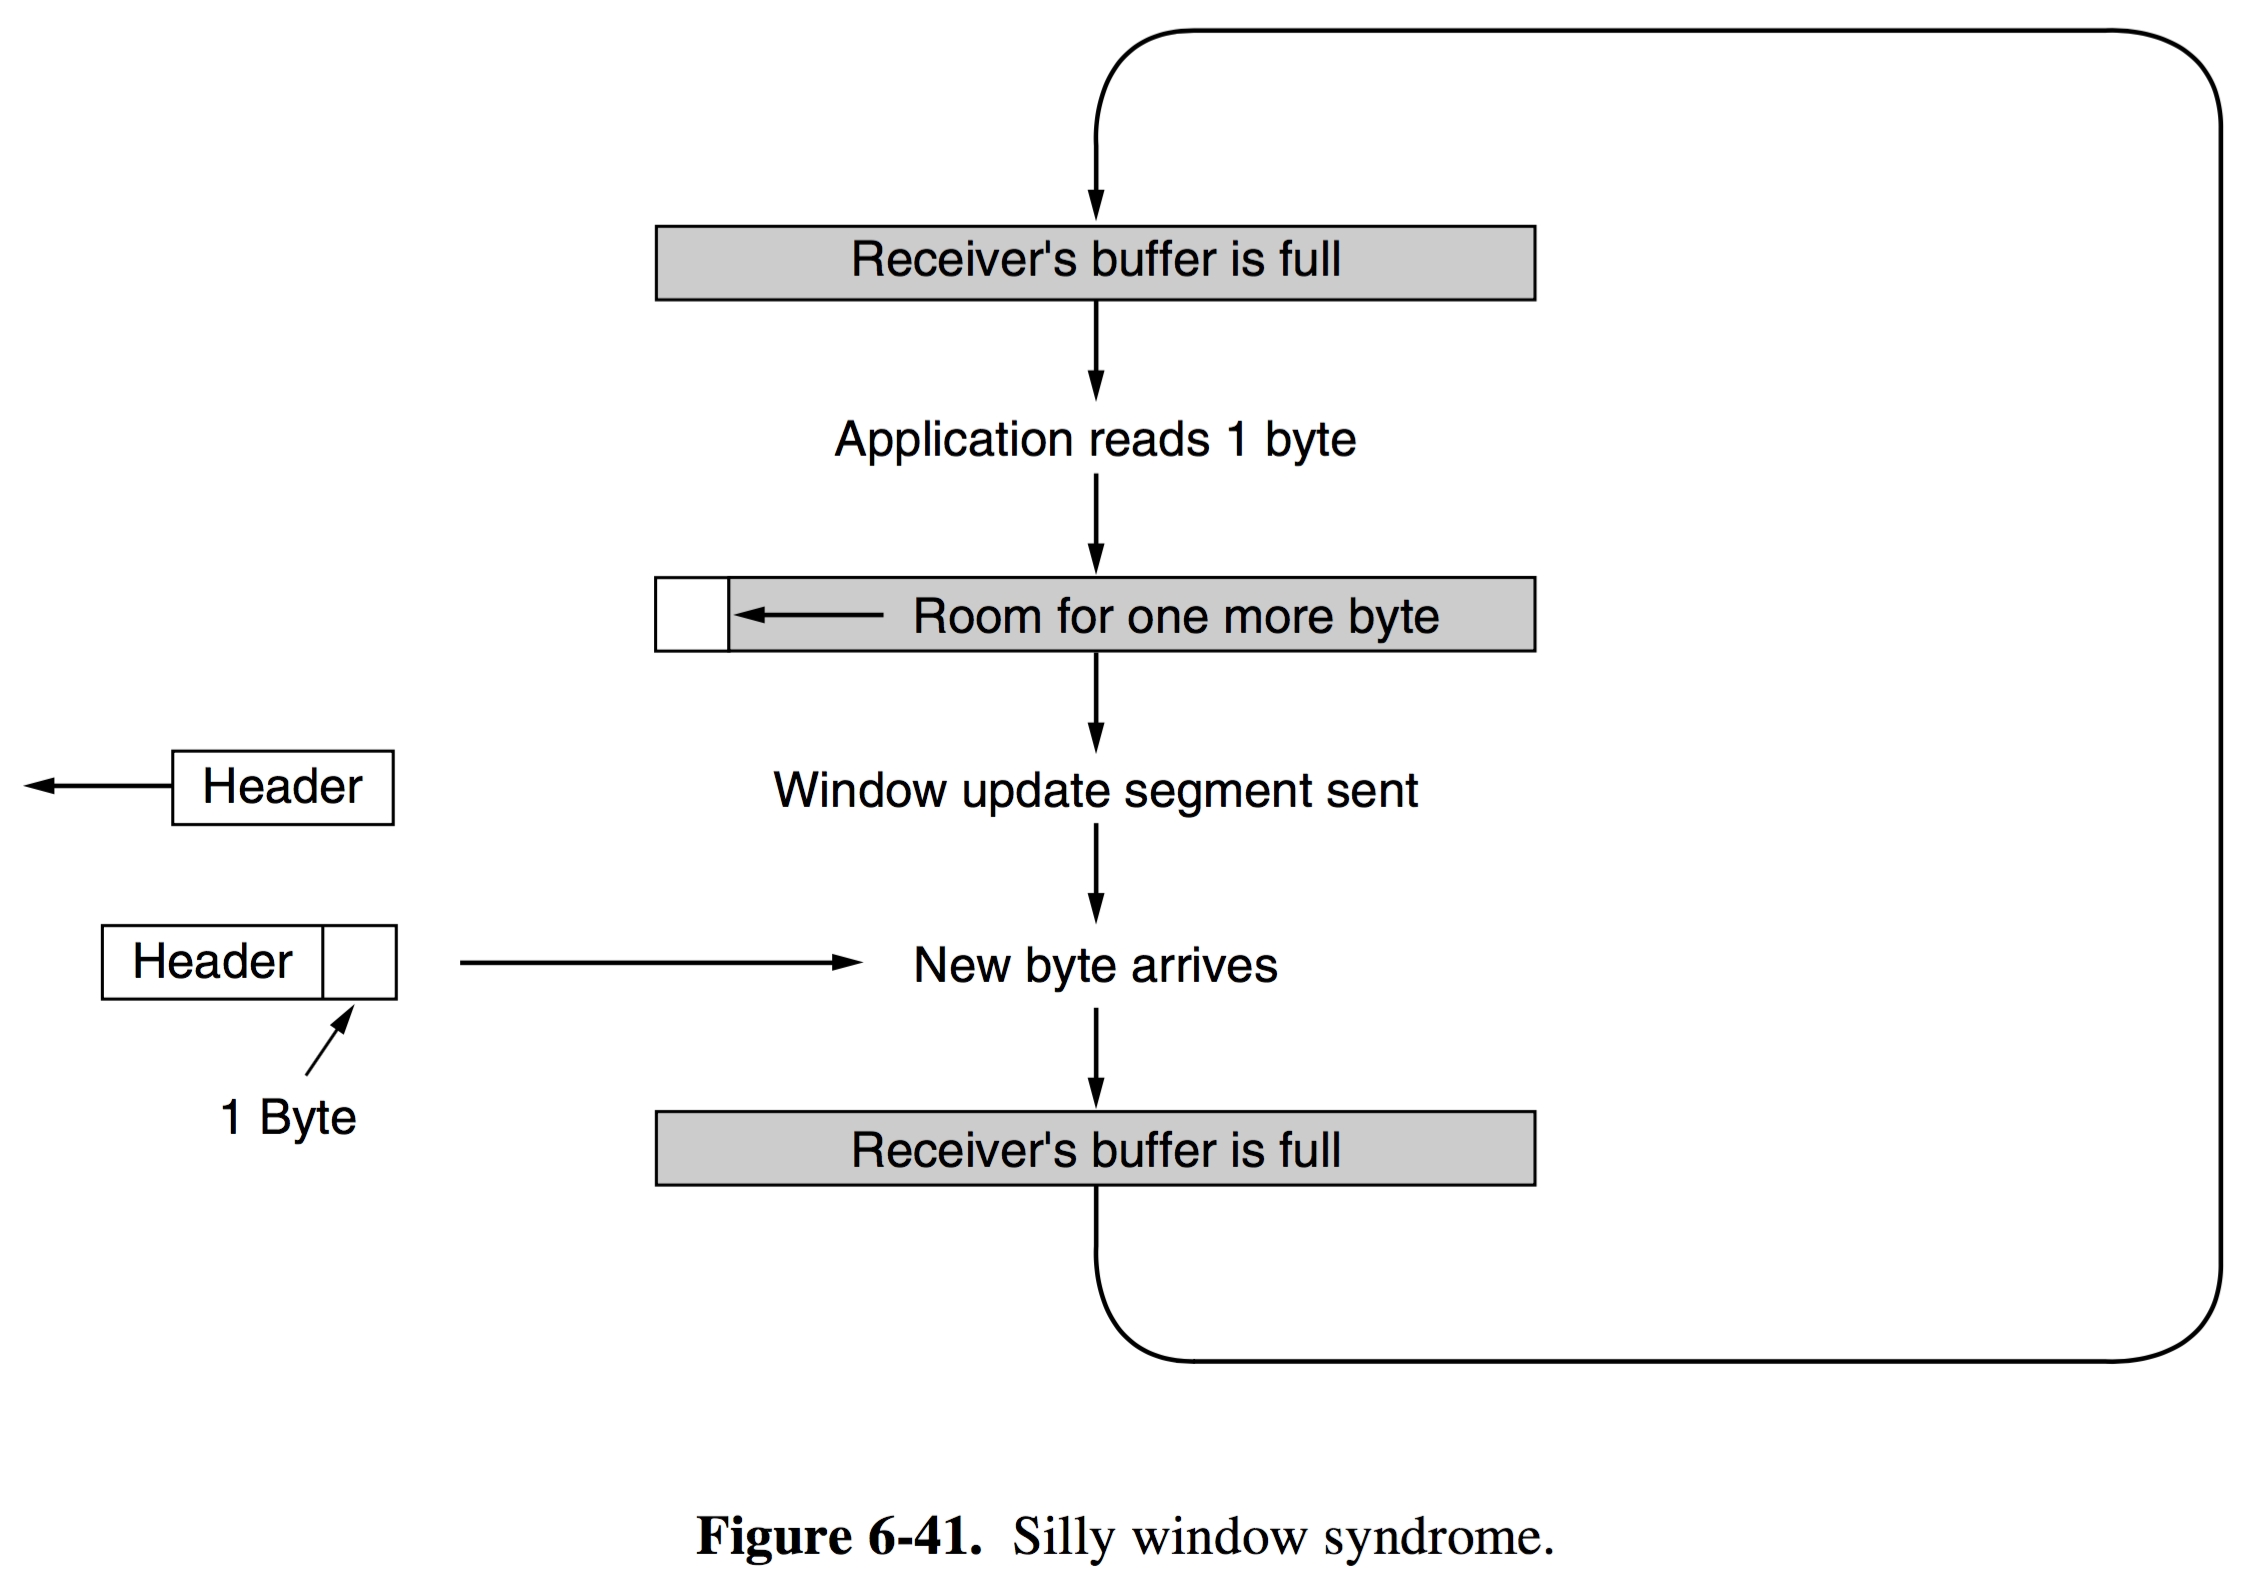
\includegraphics[width=9cm, height=6cm]{./imagenes/ventana.png}
	\end{center}

	\par Otro problema que puede arruinar el desempeño de TCP es el \textbf{síndrome de ventana tonta} (Clark). Este problema ocurre cuando se pasan datos a la entidad TCP emisora en bloques grandes, pero una aplicación interactiva del lado receptor lee datos sólo a razón de 1 byte a la vez. Para ver el problema, analice la figura 6-41. En un principio, el búfer TCP del lado receptor está lleno y el emisor lo sabe (es decir, tiene un tamaño de ventana de 0). Entonces la aplicación interactiva lee un carácter del flujo TCP. Esta acción hace feliz al receptor TCP, por lo que envía una actualización de ventana al emisor para indicar que está bien que envíe 1 byte. El emisor accede y envía 1 byte. El búfer ahora está lleno, por lo que el receptor confirma la recepción del segmento de 1 byte y establece la ventana a 0. Este comportamiento puede continuar por siempre.

	\par La solución de Clark es evitar que el receptor envíe una actualización de ventana para 1 byte. En cambio, se le obliga a esperar hasta tener disponible una cantidad decente de espacio, y luego lo anuncia. Específicamente, el receptor no debe enviar una actualización específica de ventana sino hasta que pueda manejar el tamaño máximo de segmento que anunció al establecerse la conexión, o hasta que su búfer quede a la mitad de capacidad, lo que sea más pequeño. Además, el emisor también puede ayudar al no enviar segmentos muy pequeños. En cambio, debe esperar hasta que pueda enviar un segmento completo, o por lo menos uno que contenga la mitad del tamaño del búfer del receptor.

	\par El algoritmo de Nagle y la solución de Clark al síndrome de ventana tonta son complementarios. Nagle trataba de resolver el problema causado por la aplicación emisora que entregaba datos a TCP, 1 byte a la vez. Clark trataba de resolver el problema de que la aplicación receptora tomara los datos de TCP, 1 byte a la vez. Ambas soluciones son válidas y pueden operar juntas. El objetivo es que el emisor no envíe segmentos pequeños y que el receptor no los pida.

	\par El receptor TCP también puede hacer más para mejorar el desempeño que sólo actualizar ventanas en unidades grandes. Al igual que el emisor TCP, tiene la capacidad de almacenar datos en el búfer, por lo que puede bloquear una solicitud READ de la aplicación hasta que pueda proporcionarle un bloque grande de datos. Al hacer esto se reduce la cantidad de llamadas a TCP (y la sobrecarga). También aumenta el tiempo de respuesta, pero en las aplicaciones no interactivas tales como la transferencia de archivos, la eficiencia puede ser más importante que el tiempo de respuesta a las solicitudes individuales.


\subsection{Administración de temporizadores de TCP}

	\par TCP usa varios temporizadores (al menos de manera conceptual) para hacer su trabajo. El más importante de éstos es el RTO (\textbf{Retransmission TimeOut}). Cuando se envía un segmento, se inicia un temporizador de retransmisiones. Si la confirmación de recepción del segmento llega antes de que expire el temporizador, éste se detiene. Por otro lado, si el temporizador termina antes de que llegue la confirmación de recepción, se retransmite el segmento (y se inicia de nuevo el temporizador). Surge entonces la pregunta: ¿Qué tan grande debe ser el intervalo de expiración del temporizador?

	\begin{center}
		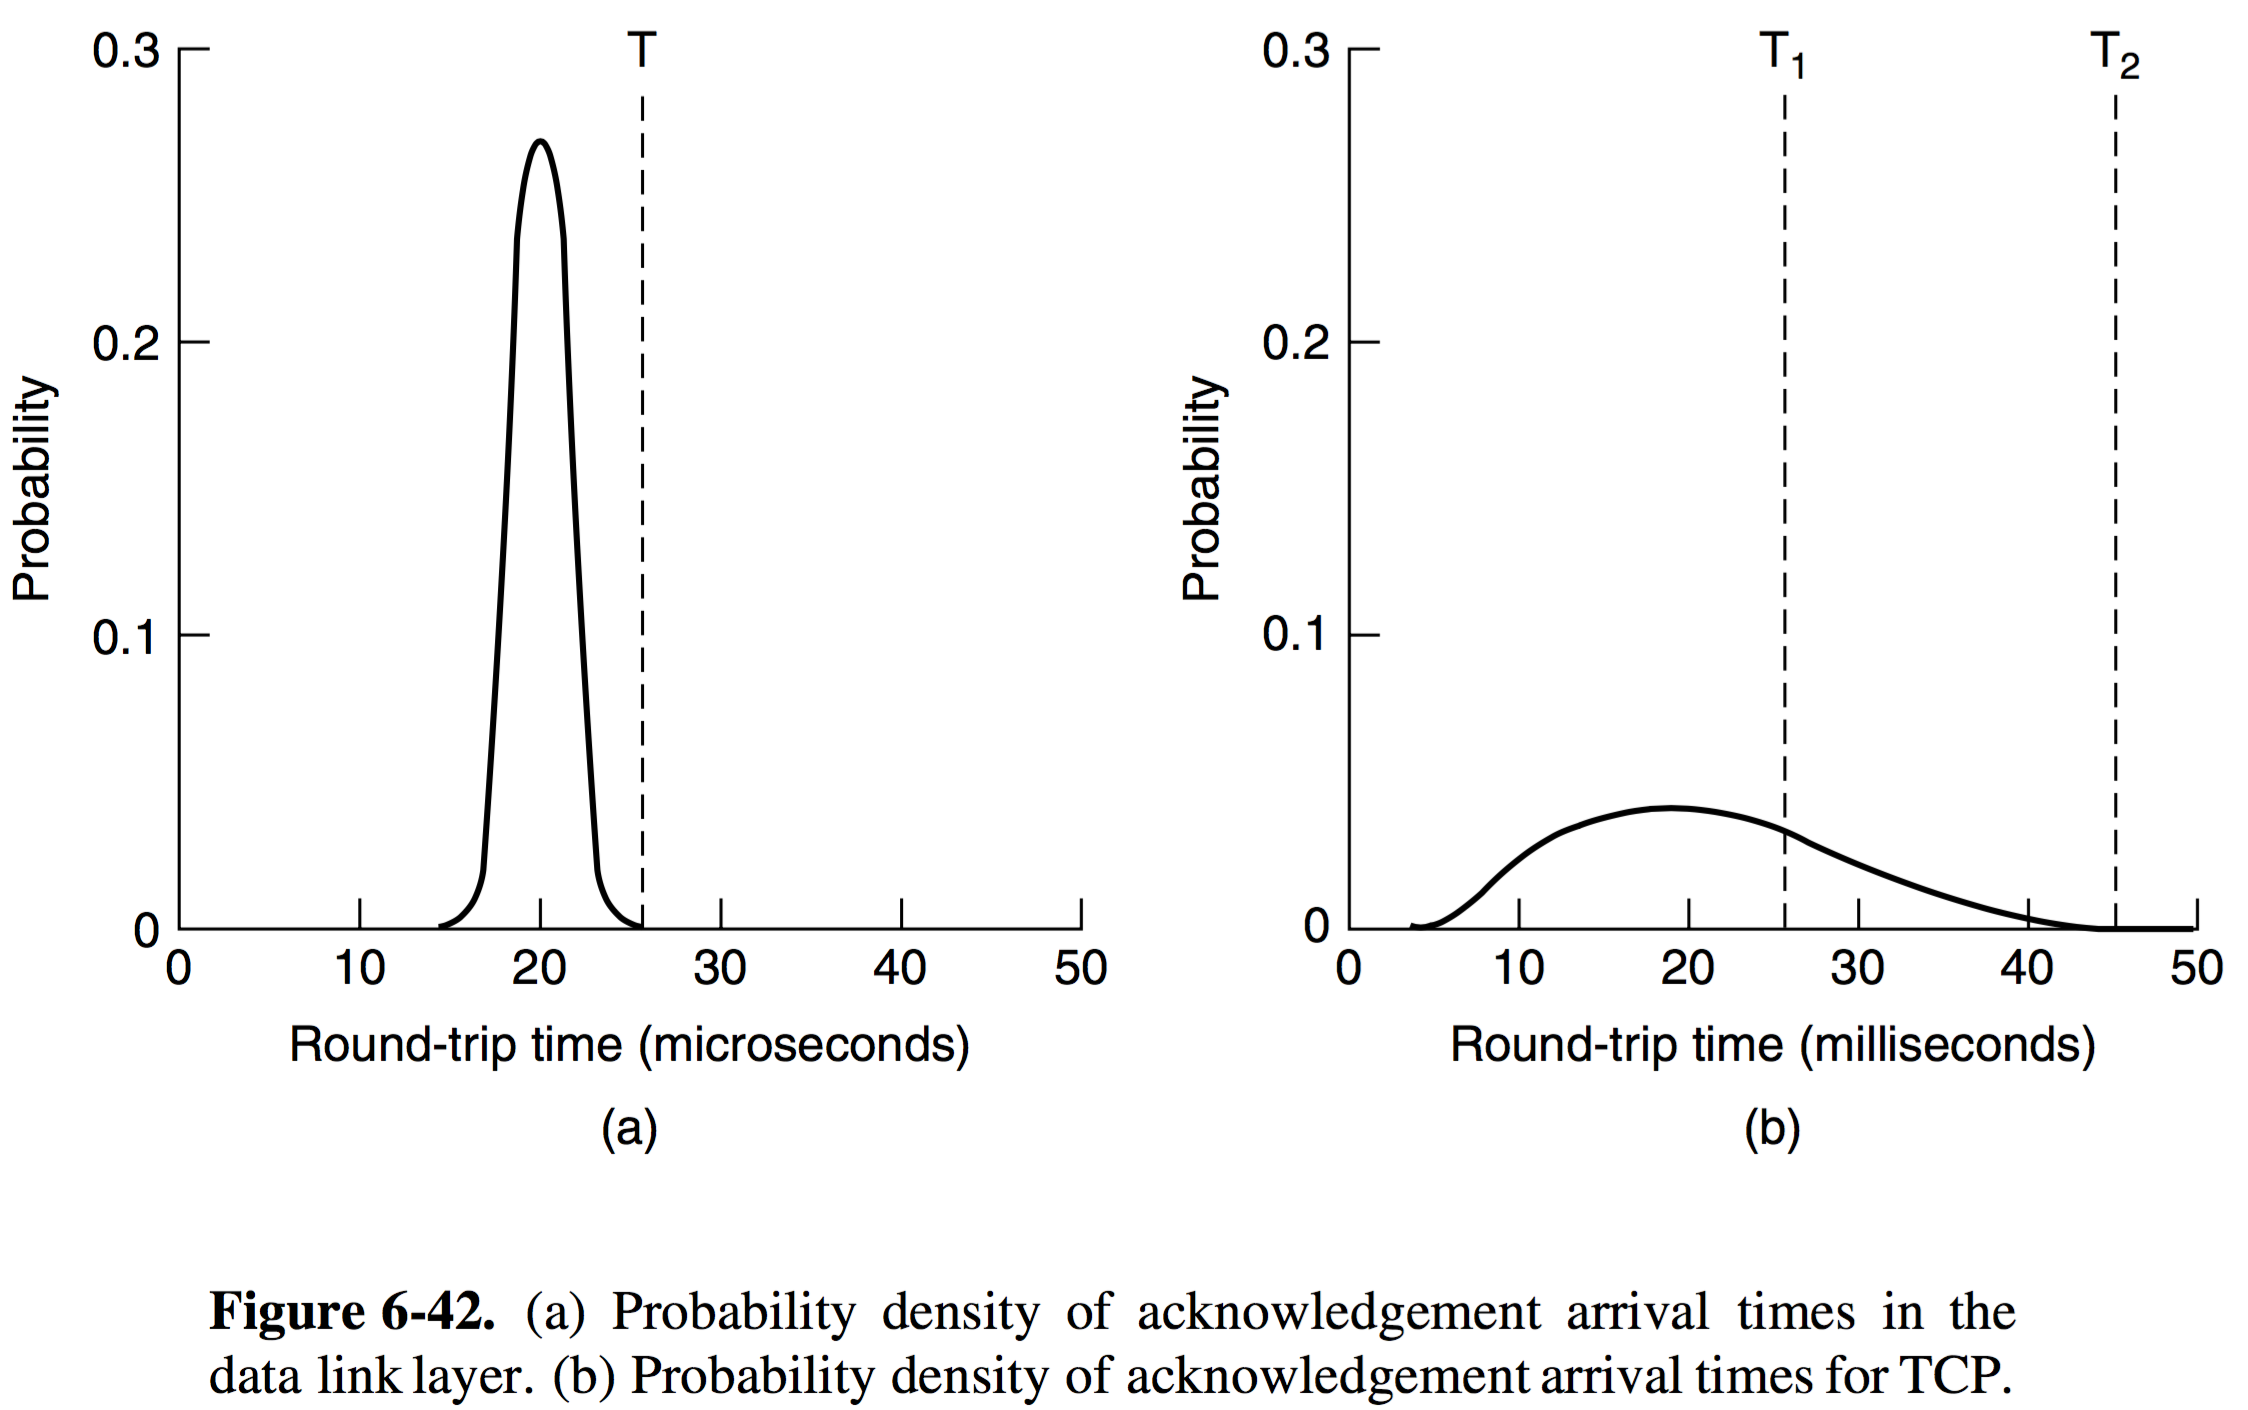
\includegraphics[width=9cm, height=6cm]{./imagenes/temporalizador.png}
	\end{center}

	\par La función de densidad de probabilidad del tiempo que tarda en regresar una confirmación de recepción TCP se parece más a la figura 6-42(b) que a la figura 6-42(a). Es más grande y variable. Es complicado determinar el tiempo de ida y vuelta al destino. Incluso cuando se conoce, es difícil decidir sobre el intervalo de expiración del temporizador. Si se establece demasiado corto, por decir \textit{T1} en la figura 6-42(b), ocurrirán retransmisiones innecesarias e Internet se llenará de paquetes inútiles. Si se establece demasiado largo (por ejemplo, \textit{T2}), el desempeño sufrirá debido al largo retardo de retransmisión de cada paquete perdido. Es más, la varianza y la media de la distribución de llegadas de confirmaciones de recepción pueden variar con rapidez en unos cuantos segundos, a medida que se generan y se resuelven congestionamientos.

	\par La solución es usar un algoritmo dinámico que ajuste de manera constante el intervalo de expiración del temporizador, con base en mediciones continuas del desempeño de la red. El algoritmo utilizado por lo general por el TCP se lo debemos a \textbf{Jacobson} y funciona de la siguiente manera. Por cada conexión, TCP mantiene una variable llamada SRTT (\textbf{Tiempo de Ida y Vuelta Suavizado}), que es la mejor estimación actual del tiempo de ida y vuelta al destino en cuestión. Al enviarse un segmento, se inicia un temporizador, tanto para ver el tiempo que tarda la confirmación de recepción como para activar una retransmisión si se tarda demasiado. Si llega la confirmación de recepción antes de expirar el temporizador, TCP mide el tiempo que tardó la confirmación de recepción, por decir R. Luego actualiza el SRTT de acuerdo con la fórmula:
	
	\begin{center}
		$ SRTT =   \alpha SRTT + (1 – \alpha ) R $
	\end{center}

	\par en donde $\alpha$ es un factor de suavizado que determina la rapidez con que se olvidan los valores anteriores. Por lo común, $\alpha = 7/8$.

	\par Incluso con un buen valor de SRTT, seleccionar la expiración adecuada del temporizador de retransmisión no es un asunto sencillo. Las primeras implementaciones de TCP usaban 2xRTT, pero la experiencia demostró que un valor constante era inflexible, puesto que no respondía cuando subía la varianza.

	\par Para corregir este problema, Jacobson propuso hacer que el valor de expiración del temporizador fuera sensible a la diferencia en los tiempos de ida y vuelta, así como al tiempo de ida y vuelta suavizado. Para este cambio hay que llevar el registro de otra variable suavizada, RTTVAR (\textbf{Variación de Tiempo de Ida y Vuelta}) que se actualiza mediante la siguiente fórmula:

	\begin{center}
		$ RTTVAR = \beta RTTVAR + (1 – \beta) | SRTT – R | $
	\end{center}	 

	\par por lo general, $\beta = 3/4$. El tiempo de expiración de retransmisión,
RTO, se establece así:

	\begin{center}
		$ RTO = SRT + 4 RTTVAR $
	\end{center}

\par La elección del factor 4 es un tanto arbitraria, pero se puede hacer la multiplicación por 4 con un solo desplazamiento y menos de 1\% de todos los paquetes llegan después de más de cuatro desviaciones estándar. Observe que RTTVAR no es exactamente lo mismo que la desviación estándar (en realidad es la desviación media), pero es lo bastante parecida en la práctica.	
	
	\par Un problema que ocurre con la recopilación de las muestras, R, del tiempo de ida y 
	vuelta es qué hacer cuando expira el temporizador de un segmento y se envía de 
	nuevo. Cuando llega la confirmación de recepción, no está claro si ésta se refiere a la 
	primera transmisión o a una posterior. Si adivinamos mal se puede contaminar 
	seriamente el temporizador de retransmisión. Karn hizo una propuesta sencilla: no 
	actualizar las estimaciones sobre ninguno de los segmentos retransmitidos. Además, se 
	duplicará el tiempo de expiración con cada retransmisión sucesiva hasta que los 
	segmentos pasen a la primera. La mayoría de las implementaciones de TCP lo utilizan.
	
	\par El temporizador de retransmisiones no es el único temporizador que TCP utiliza. El \textbf{temporizador de persistencia} es el segundo de ellos. Está diseñado para evitar el siguiente interbloqueo.
	\begin{enumerate}
		\item  El receptor envía una confirmación de recepción con un tamaño de ventana de 0 para indicar al emisor que espere.
		\item Después el receptor actualiza la ventana, pero se pierde el paquete con la actualización.
		\item Ahora, tanto el emisor como el receptor están esperando a que el otro haga algo.
	\end{enumerate}	
	
	\par Cuando expira el temporizador de persistencia, el emisor transmite un sondeo al receptor. La respuesta al sondeo proporciona el tamaño de la ventana. Si aún es cero, se inicia el temporizador de persistencia una vez más y se repite el ciclo. Si es diferente de cero, ahora se pueden enviar datos.

	\par Un tercer temporizador que utilizan algunas implementaciones es el \textbf{temporizador de seguir con vida} (\textit{keepalive}). Cuando una conexión ha estado inactiva durante demasiado tiempo, el temporizador de seguir con vida puede expirar para ocasionar que un lado compruebe que el otro aún está ahí. Si no se recibe respuesta, se termina la conexión. Esta característica es controversial puesto que agrega sobrecarga y puede terminar una conexión saludable debido a una partición temporal de la red.

\subsection{Control de congestión en TCP}

	\par Cuando la carga ofrecida a cualquier red es mayor que la que puede manejar, se genera una congestión. Internet no es ninguna excepción. La capa de red detecta la congestión cuando las colas crecen demasiado en los enrutadores y trata de lidiar con este problema, aunque lo único que haga sea descartar paquetes. Es responsabilidad de la capa de transporte recibir la retroalimentación de congestión de la capa de red y reducir la tasa del tráfico que envía a la red. En Internet, TCP desempeña el papel principal en cuanto al control de la congestión, así como en el transporte confiable. Por esto se le considera un protocolo tan especial.
	
	\par El primer paso del manejo de congestión es su detección. La expiración de un temporizador causada por un paquete perdido podía deberse a ruido en la línea de transmisión o el descarte de paquetes en el enrutador congestionado.  Hoy en día la pérdida de paquetes por errores de transmisión es relativamente rara debido a que las troncales de larga distancia son de fibra (aunque las redes inalámbricas son otra historia). En consecuencia, la mayoría de las expiraciones de tiempo en Internet se deben a la congestión. Todos los algoritmos de congestión de TCP suponen que las expiraciones de tiempo son causados por congestión y las revisan en busca de problemas.
	
\subsubsection{¿Qué hace TCP para evitar la pérdida de segmentos?}

	\begin{itemize}
		\item  \underline{Solución 1:} al establecerse una conexión se tiene que seleccionar un tamaño de ventana adecuado. El receptor puede especificar una ventana con base en su tamaño de búfer. Si el emisor se ajusta a su tamaño de ventana, no ocurrirán problemas por desbordamiento de búferes en la terminal receptora, pero si podrán ocurrir en la red interna por su propia congestión. En la parte a) de la figura vemos un tubo grueso que conduce a un receptor de poca capacidad. Mientras el emisor no envíe más agua de la que puede contener la cubeta, no se perderá agua. En la parte b) de la figura el factor limitante no es la capacidad de la cubeta sino la capacidad de conducción interna de la red. Si entra demasiada agua a alta velocidad, ésta retrocederá, perdiéndose algo (en este caso, por el desbordamiento del embudo).

	\begin{center}
		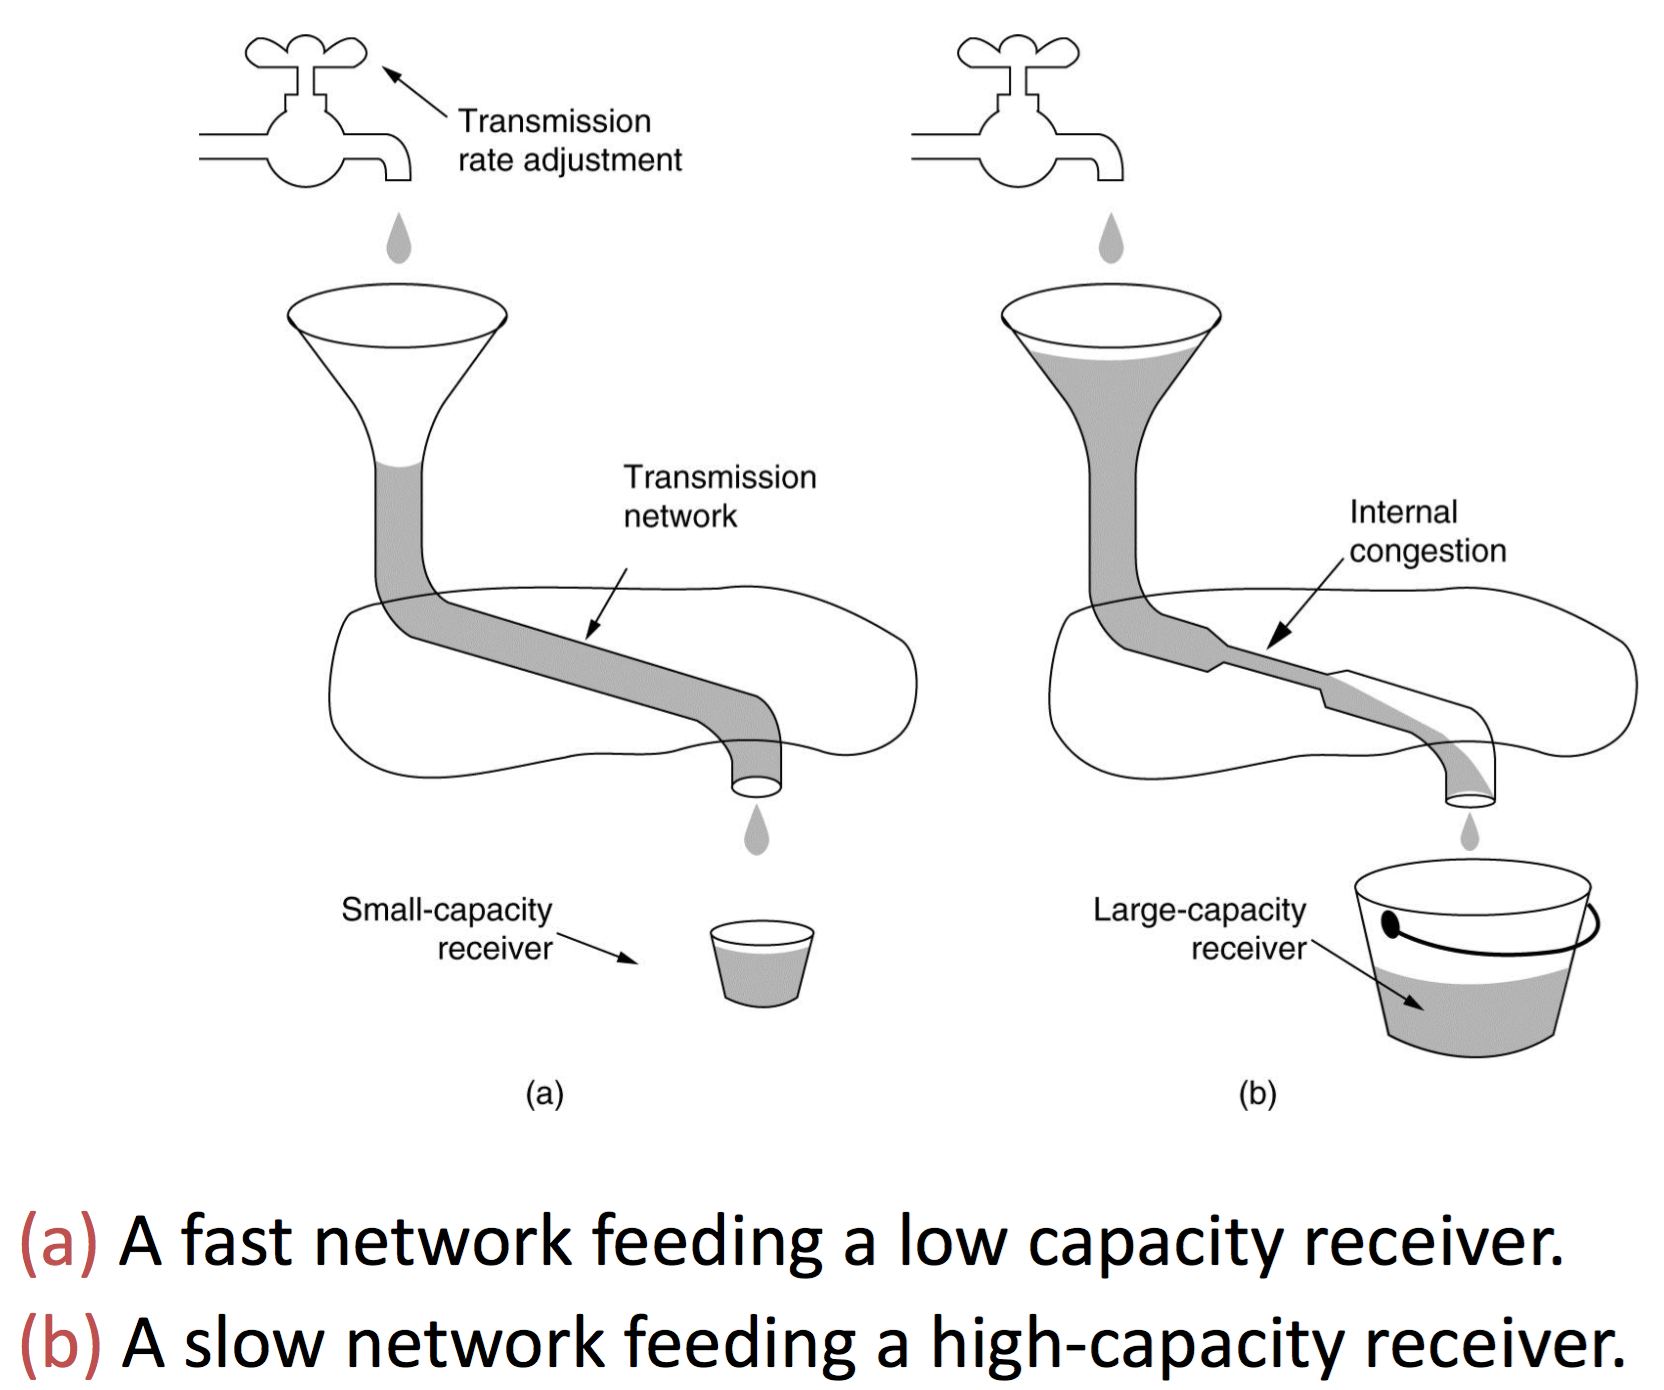
\includegraphics[width=7cm, height=5cm]{./imagenes/sol1.png} 
	\end{center}

	\item \underline{Solución 2:} aceptar que existen dos problemas potenciales (capacidad de la red y capacidad del receptor) y manejarlos por separado. Para ello cada emisor mantiene dos ventanas:  la ventana que ha otorgado el receptor, y una segunda ventana, la ventana de congestión. Cada una refleja la cantidad de bytes que puede enviar el emisor. La cantidad de bytes que pueden enviarse es la cifra menor de las dos ventanas, por lo tanto, la ventana efectiva es el mínimo de lo que el emisor piensa que es correcto y lo que el receptor piensa que está bien. Si el receptor dice “envía a 8 KB” y el emisor sabe que las ráfagas de haste 32 KB pueden llegar sin problemas, envía los 8 KB solicitados.

	\item \underline{Solución 3:} \textbf{Algoritmo de arranque lento} (Jacobson 1988). 	
		\par Es requerido para todas las implementaciones de TCP. Al establecer una conexión el emisor asigna a la ventana de congestión el tamaño de segmento máximo usado por la conexión, entonces envía un segmento máximo. Si se recibe la confirmación de este segmento antes que expire el temporizador, el emisor agrega el equivalente en bytes de un segmento a la ventana de congestión para hacerla de dos segmentos de tamaño máximo y envía dos segmentos. A medida que se confirma cada uno de estos segmentos, se aumenta el tamaño de la ventana de congestión en un segmento máximo.
	
	\par Cuando la ventana de congestión es de \textit{N} segmentos, si de todos los \textit{N} se reciben confirmaciones de recepción a tiempo, se aumenta la ventana de congestión en la cuenta de bytes correspondiente a \textit{N} segmentos. De hecho, cada ráfaga confirmada duplica la ventana de congestionamiento. La ventana de congestión sigue creciendo exponencialmente hasta ocurrir una expiración del temporizador o alcanzar el tamaño de la ventana receptora. La idea es que si las ráfagas de 1024, 2048 y 4096 bytes funcionan bien, pero una ráfaga de 8192 produce una expiración del temporizador, la ventana de congestión debe establecerse a 4096 para evitar la congestión. Mientras el tamaño de la ventana de congestión permanezca en 4096, no se enviará una ráfaga de mayor longitud, sin importar el espacio de ventana otorgada por el receptor.

	\par Recortar la ventana de congestión a la mitad porque hubo una expiración de temporizador y quedarse ahí, puede ser demasiado, porque puede ser que la red tenga una capacidad mayor a esa mitad y así se desaprovecharía esa capacidad de la subred. Comenzar arranque lento cada vez que expira un temporizador sería demasiado, y sería posible una recuperación mucho más rápida, al menos en la mayoría de los casos.

	\item \underline{Solución 4:} \textbf{Algoritmo de control de congestión de Internet} (o TCP Talhoe).
	
		\par Utiliza un tercer parámetro, el \textbf{umbral}, inicialmente de 64 KB, además de las ventanas de recepción y congestión. Al ocurrir una expiración del temporizador, se establece un umbral en la mitad de la ventana de congestión actual, y la ventana de congestión se restablece a un segmento máximo. Luego se usa el arranque lento para determinar lo que puede manejar la red, excepto que el crecimiento exponencial termina al alcanzar el umbral. A partir de ese punto las transmisiones exitosas aumentan linealmente la ventana de congestión (en un segmento máximo por ráfaga) en lugar de uno por segmento. En efecto, este algoritmo está suponiendo que probablemente es aceptable recortar la ventana de congestión a la mitad, y luego aumentarla gradualmente a partir de ahí.

	\par Si no ocurren más expiraciones de temporizador, la ventana de congestión continuará creciendo hasta el tamaño de la ventana del receptor. En ese punto dejará de crecer y permanecerá constante mientras no ocurran más expiraciones de temporizador y la ventana del receptor no cambie de tamaño. Notar cómo se baja la tasa de transferencia luego de un \textit{timeout}. Este método resuelve el problema 1 del arranque lento, pero no el problema 2.

	\begin{center}
		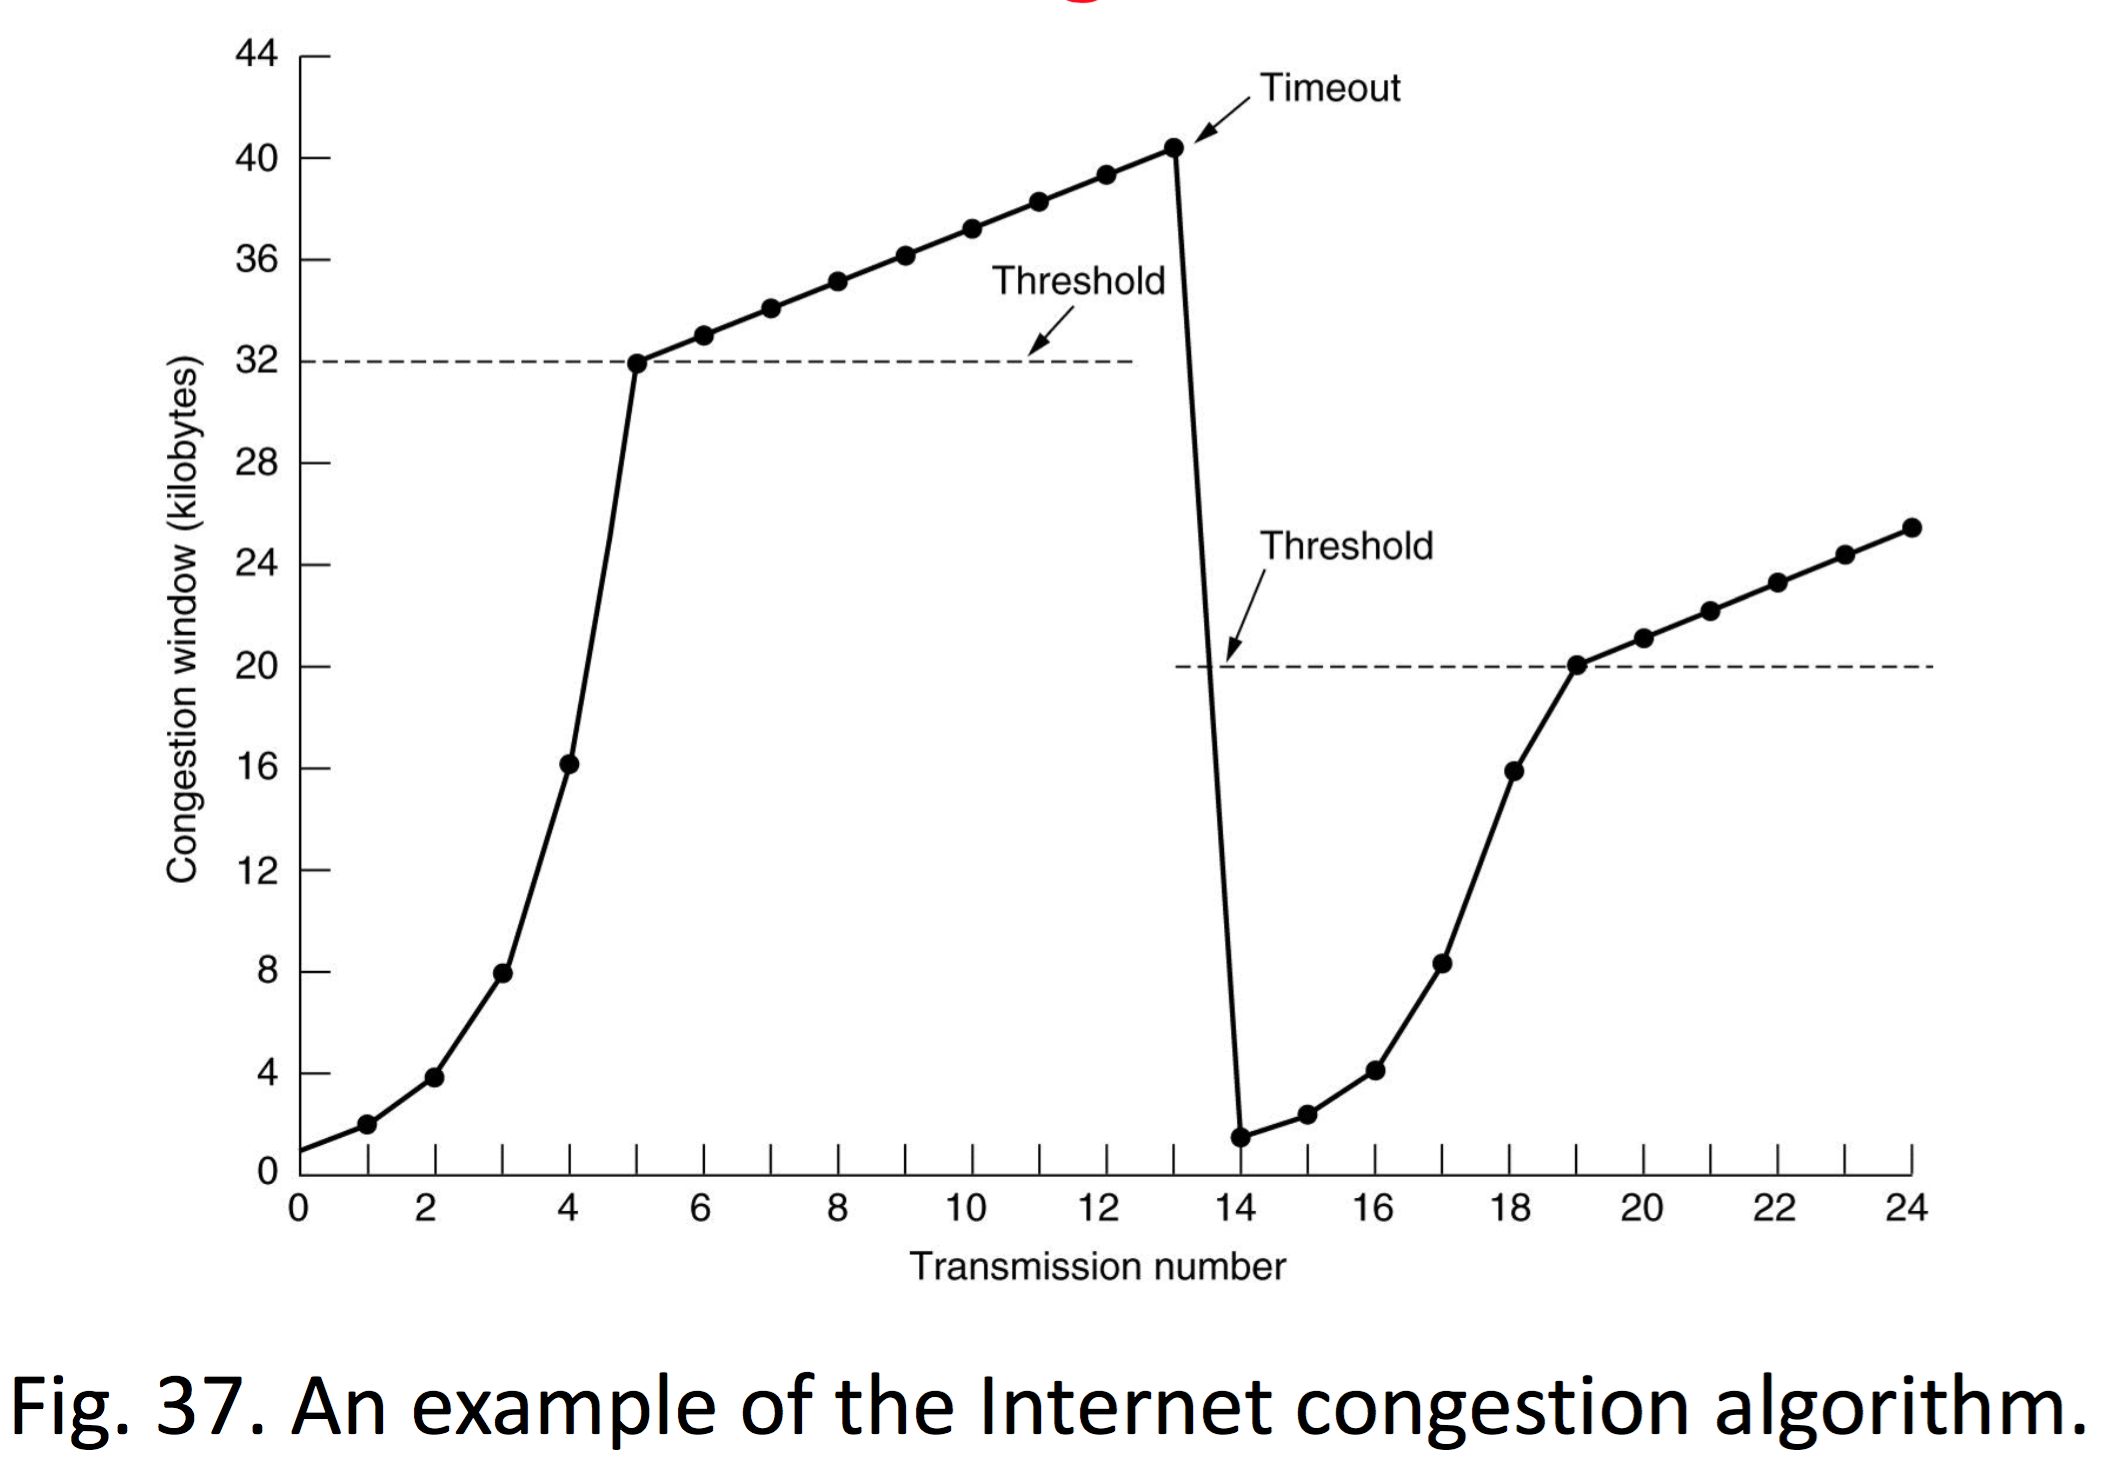
\includegraphics[width=7cm, height=5cm]{./imagenes/sol4.png} 
	\end{center}

	\par En la figura 37 el tamaño de segmento es de 1024 bytes. Inicialmente la ventana de congestón era de 64 KB, pero ocurre una expiración del temporizador, así que se establece el umbral a 32 KB y la ventana de congestión en 1 KB, para la transmisión 0. La ventana de congestión entonces crece exponencialmente hasta alcanzar el umbral (32 KB). A partir de entonces crece linealmente. La transmisión 13 tiene mala suerte y ocurre una expiración del temporizador. Se establece el umbral en la mitad de la ventana actual (ahora de 40 KB, por lo que la mitad es de 20 KB), e inicia de nuevo el arranque lento. Al llegar las confirmaciones de recepción de la transmisión 14, los primeros 4 incrementan la ventana de congestión en un segmento máximo, pero después de eso el crecimiento se vuelve lineal nuevamente.

	\item \underline{Solución 5:} \textbf{Algoritmo de TCP Reno}.
	\par Evitar arranque lento (excepto cuando la conexión es comenzada) cuando expira el temporizador de reenvíos. Luego de iniciada la conexión se comienza con arranque lento. A continuación la ventana de congestión crece linealmente hasta que se detecta una pérdida de paquete. El paquete perdido es retransmitido y se usa recuperación rápida. Luego la ventana de congestión de una conexión se achica a la mitad durante un RTT (\textit{decrecimiento multiplicativo}) y luego la ventana de congestión va incrementando de a un segmento por cada RTT (\textit{crecimiento aditivo}). Este comportamiento continua indefinidamente. Luego se hicieron ajustes menores a TCP Reno.

	\begin{center}
		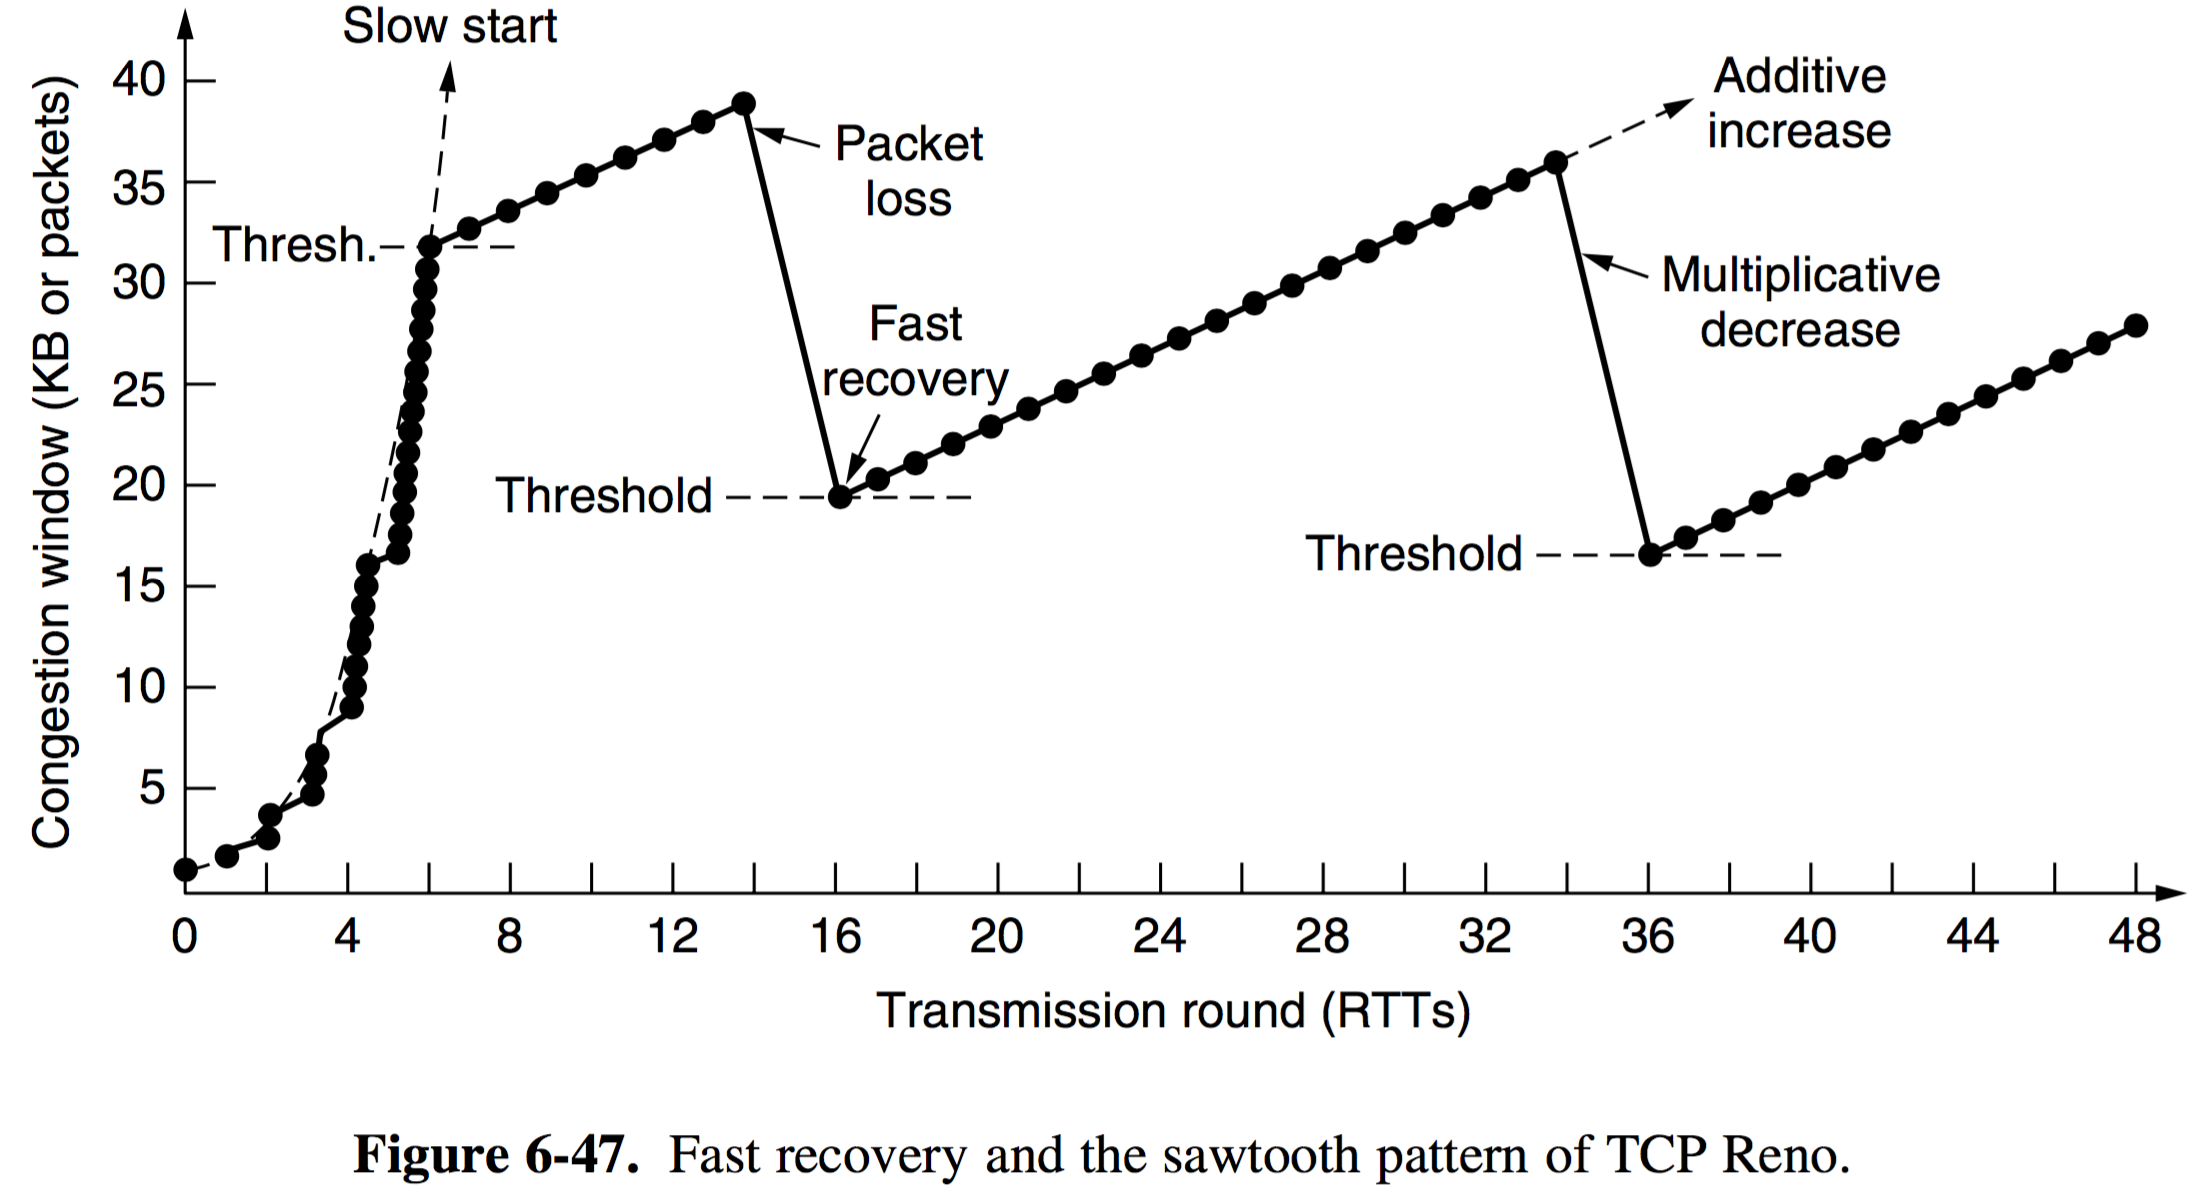
\includegraphics[width=7cm, height=5cm]{./imagenes/sol5.png} 
	\end{center}

	\end{itemize}


\chapter{LA CAPA DE APLICACIÖN}

	\section{World Wide Web}
	
		\par La web, popularmente conocida como \textit{World Wide Web}, es un marco arquitectónico para acceder a cierto contenido vinculado distribuido en millones de máquinas por toda Internet. En 1994, el CERN y el MIT firmaron un acuerdo para establecer el \textbf{W3C} (\textit{World Wide Web Consortium}), una organización dedicada al desarrollo de web, a la estandarización de protocolos.
		
		\subsection{Panorama de la aquitectura}
		
			\par Desde el punto de vista del usuario, la web consiste en una enorme colección de contenido en forma de páginas web, por lo general, conocidas simplemente como páginas. Cada una puede contener vínculos a otras páginas en cualquier lugar del mundo. Para seguir un vínculo, los usuarios pueden hacer clic en él, y a continuación los llevará a la página apuntada. Este proceso se puede repetir de manera indefinida. La idea de hacer que una página apunte a otra, lo que ahora se conoce como \textbf{hipertexto}.
			
			\par Por lo general, las páginas se ven mediante un programa llamado navegador. Firefox, Internet Explorer y Chrome son ejemplos de navegadores populares. El navegador obtiene la página solicitada, interpreta el contenido y despliega la página en pantalla con el formato adecuado.
			
			\begin{center}
				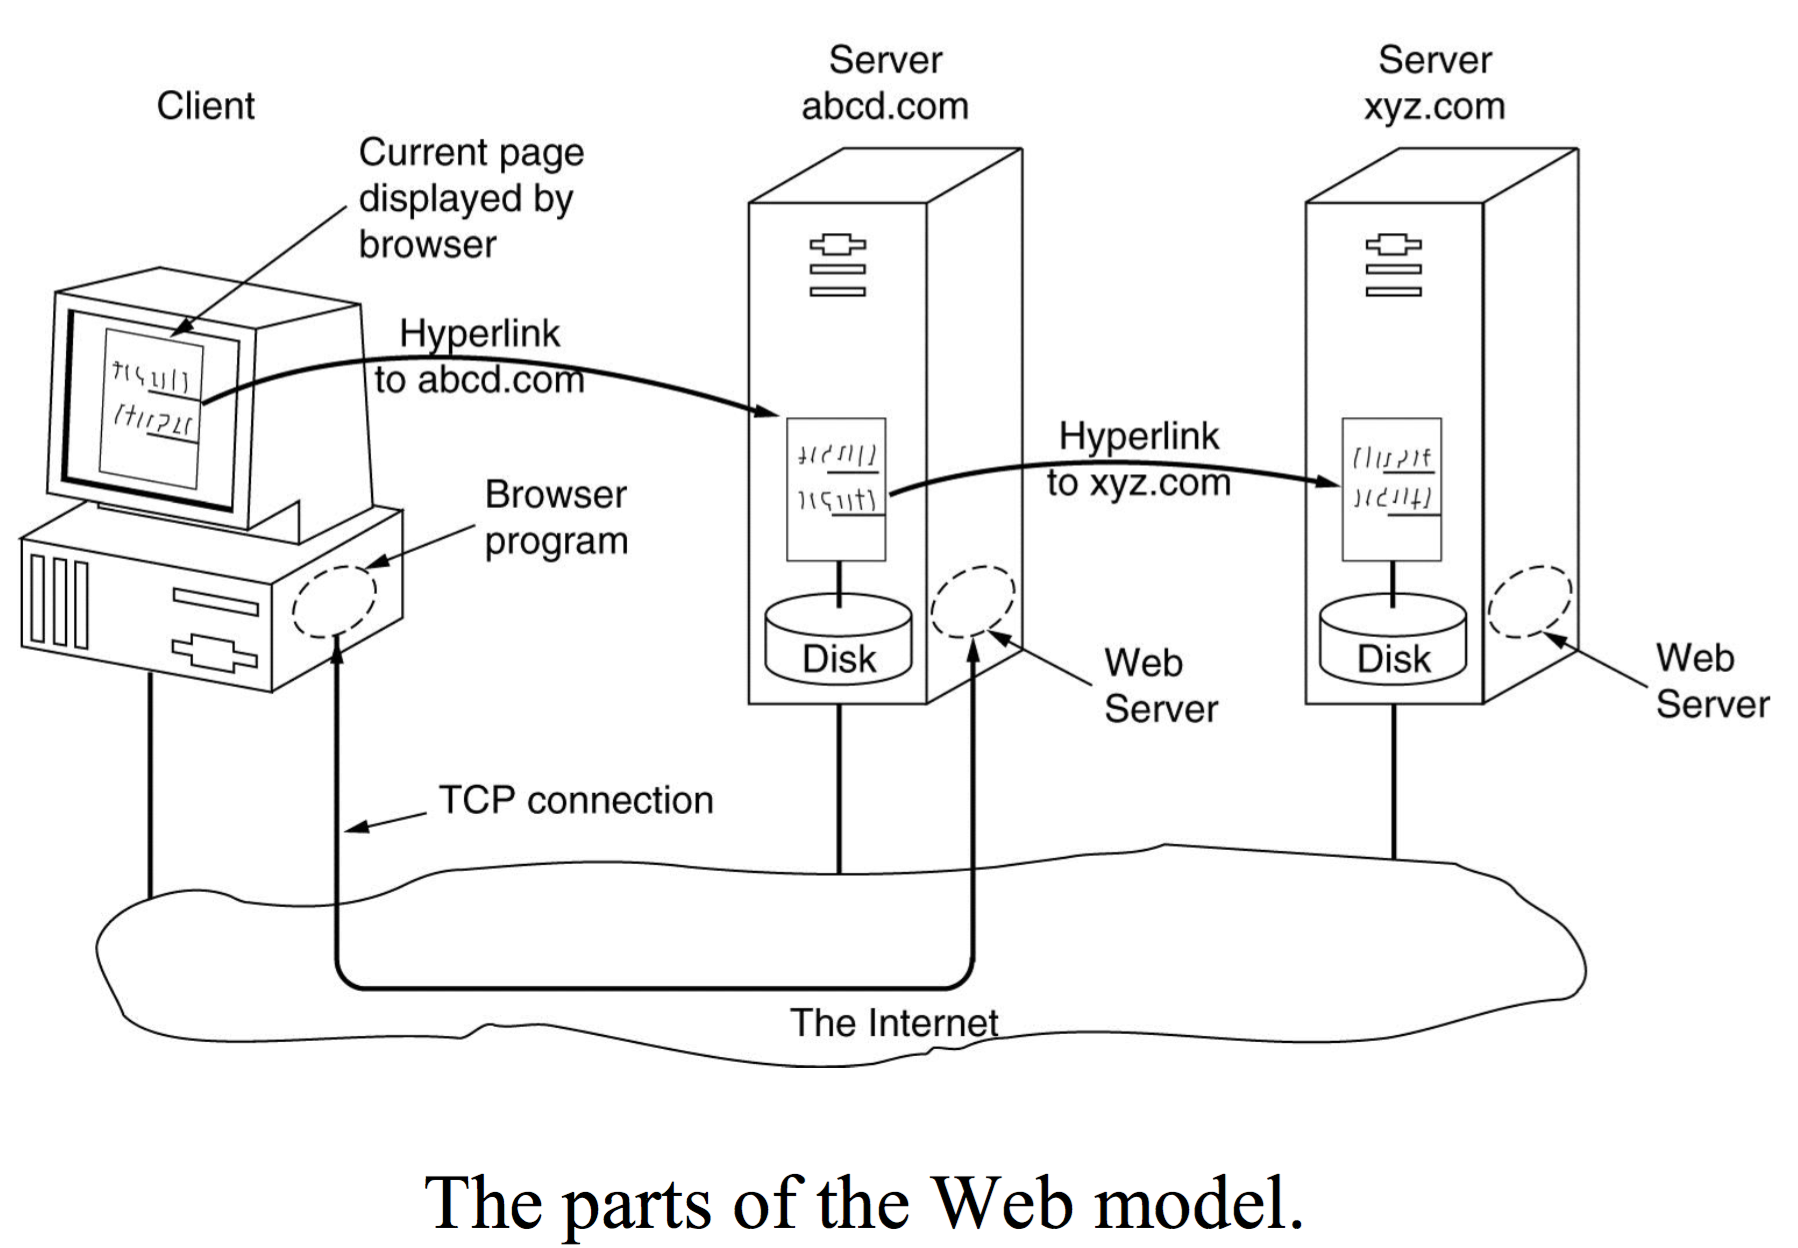
\includegraphics[width=9cm, height=5cm]{./imagenes/web.png} 
			\end{center}
			
			\subsubsection{El lado del cliente}
						
				\par Un hipervínculo incrustado en una página web necesita una manera de nombrar cualquier página que se encuentre en la web. Las páginas se nombran usando URLs (Localizadores Uniformes de Recursos), los cuales tienen tres partes:

				\begin{enumerate}
					\item El nombre del protocolo, en este caso es HTTP.
					\item Un nombre DNS de la máquina donde se localizala página.
					\item El nombre del archivo que contiene la página.
				\end{enumerate}

			\par Cuando un usuario hace click en un vínculo, el navegador sigue los siguientes pasos:
				\begin{enumerate}
					\item El navegador determina el URL
					\item El navegador pide al DNS la dirección IP del nombre DNS del URL.
					\item El DNS responde con la dirección IP.
					\item El navegador hace una conexión TCP con el puerto 80 en la dirección IP.
					\item El navegador envía un mensaje en el que solicita el archivo del URL.
					\item El servidor envía el archivo solicitado al navegador.
					\item Se libera la conexión TCP.
					\item El navegador despliega todo el texto del archivo.
					\item El navegador obtiene y despliega todas las imágenes del archivo.
				\end{enumerate}

			\subsubsection{Tipos MIME}

				\par Para poder desplegar una página el navegador tiene que entender su formato. Para permitir que todos los navegadores entiendan todas las páginas web, estas se escriben en un lenguaje estandarizado llamado HTML. Las páginas web pueden tener íconos, figuras, fotos, tablas; cada uno de estos puede enlazarse a otras páginas.

				\par El navegador es básicamente un intérprete HTML. La mayoría de los navegadores tiene varios botones y características para facilitar la navegación web. Botones para ir a la página anterior y a la página siguiente, establecer un marcador (\textit{bookmark}), ver la lista de marcadores. Las páginas también pueden guardarse en disco e imprimirse.
				
				\par No todas las páginas necesitan contener HTML. Una página puede consistir de un video en formato MPEG, un documento en formato PDF, una fotografía en formato JPEG, una canción en formato MP3 o cualquiera de cientos de otros tipos de archivos. Como las páginas HTML estándar pueden vincular a cualquiera de estos elementos, el navegador tiene un problema cuando llega a una página que no sabe cómo interpretar.

				\par En vez de hacer los navegadores cada vez más grandes al construir intérpretes para una colección extensa de tipos de archivos que aumenta con rapidez, la mayoría de los navegadores han elegido una solución más general. Cuando un servidor devuelve una página, también devuelve cierta información adicional sobre ella. Esta información incluye el tipo MIME de la página. Las páginas de tipo \textit{text/html} sólo se despliegan directamente, al igual que las páginas en unos cuantos tipos integrados más. Si el tipo MIME no es de los integrados, el navegador consulta su tabla de tipos MIME para determinar cómo desplegar la página. Esta tabla asocia los tipos MIME con los visores.

				\par Existen dos posibilidades: complementos (\textit{plug-ins}) y aplicaciones auxiliares. Un \textit{plug-in} es un módulo de código de terceros que se instala como una extensión para el navegador. Como los complementos se ejecutan dentro del navegador, tienen acceso a la página actual y pueden modificar su apariencia.
				
				\par Para poder usar un plug-in primero debe instalarse. El navegador tiene un directorio de plug-ins, donde se lo coloca. Además se registra el tipo MIME del plug-in para poder asociarlo con este. Cada navegador tiene un conjunto de procedimientos que todos los plug-in tienen que implementar a fin de que el navegador pueda llamarlos (la \textit{ interfaz del plug-in}).

				\par El navegador pone a disposición de los plug-in un conjunto de sus procedimientos, llamados \textbf{interfaz del navegador}. Los procedimientos comunes en la interfaz del navegador son para asignar y liberar memoria, desplegar un mensaje en la línea de estado del navegador y consultar al navegador sobre los parámetros. Después de que el plug-in ha hecho su trabajo, se lo elimina de la memoria del navegador.
				
				\par Otra forma de ampliar el navegador es con el uso de aplicaciones auxiliares. Estas son programas completos que se ejecutan como procesos
independientes. Las aplicaciones auxiliares no ofrecen interfaz al navegador ni usan servicios de este, por lo general solo aceptan el nombre de un archivo de trabajo y lo abren y despliegan. Ejemplos de aplicaciones auxiliares son Acrobat Reader y Microsoft Word.

				\par Muchas aplicaciones auxiliares usan el tipo MIME \textit{application}. Como consecuencia se ha definido un número considerable de subtipos para que los utilicen; por ejemplo, \textit{application/vnd.ms-powerpoint} para los archivos de PowerPoint. Las aplicaciones ayudantes no están restringidas al uso del tipo MIME \textit{application}. Por ejemplo, Adobe Photoshop usa \textit{image/x-photoshop}.
				
				\begin{center}
					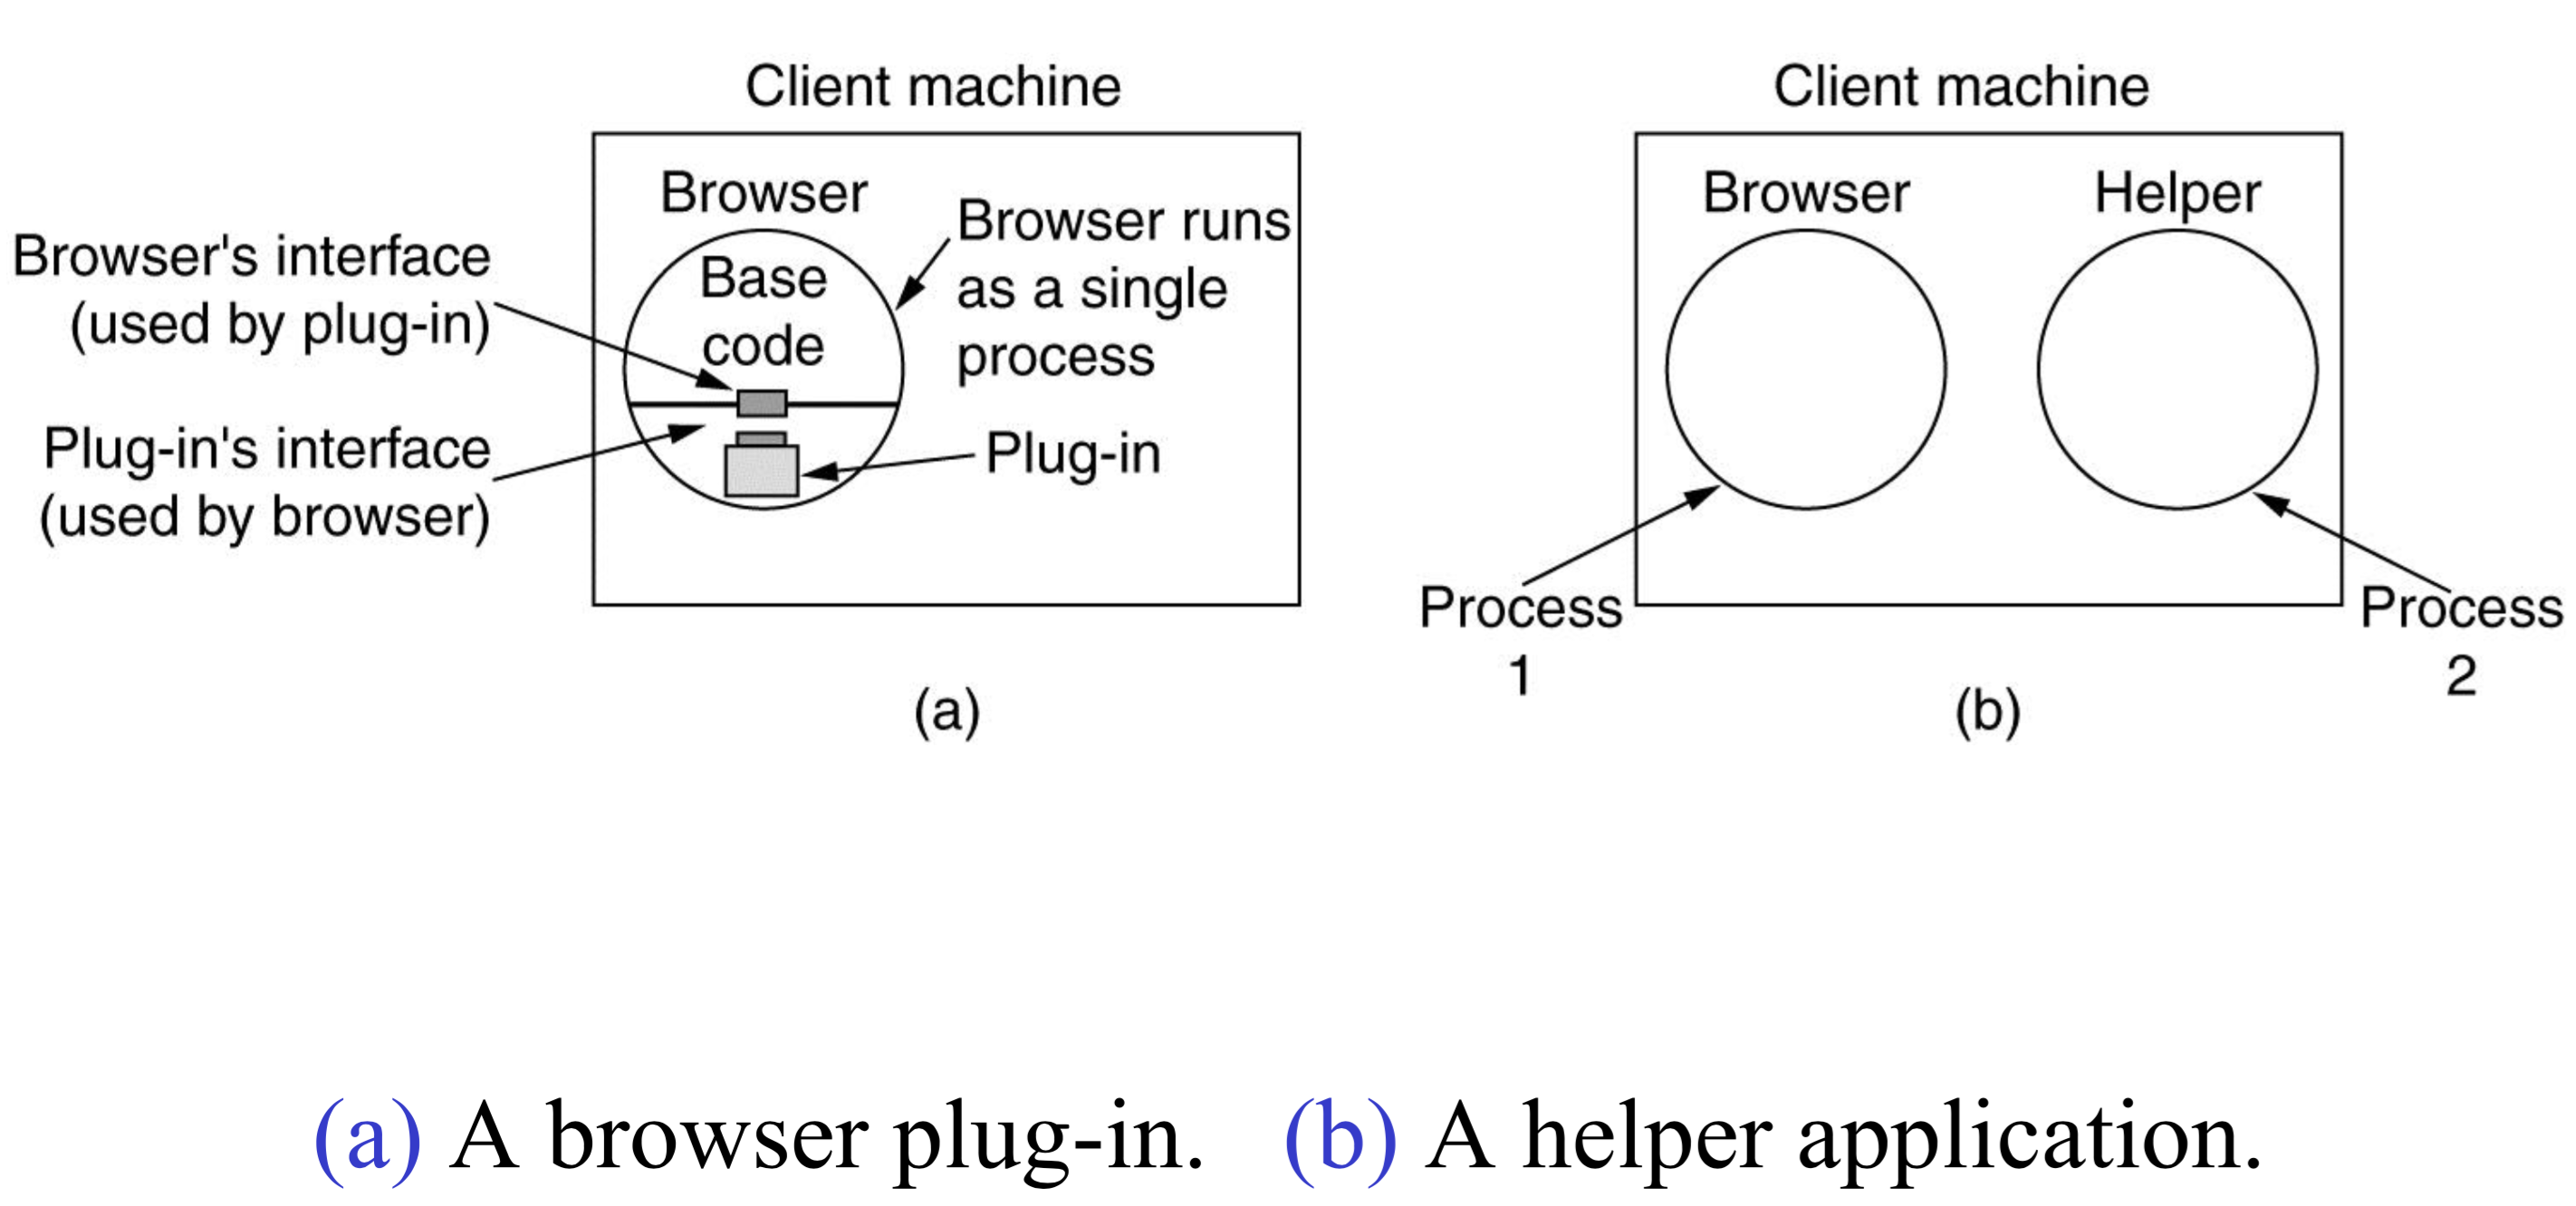
\includegraphics[width=9cm, height=5cm]{./imagenes/plugin.png} 
				\end{center}
		
			\subsubsection{El lado del servidor}
			
				\par Un servidor web  recibe el nombre de un archivo que debe buscar y devolver a través de la red. En ambos casos, los pasos que el servidor realiza en su ciclo principal son:

				\begin{enumerate}
					\item Aceptar una conexión TCP de un cliente (un navegador).
					\item Obtener la ruta a la página, que viene siendo el nombre del archivo solicitado.
					\item Obtener el archivo (del disco).
					\item Enviar el contenido del archivo al cliente.
					\item Liberar la conexión TCP.
				\end{enumerate}	

				\par En el diseño anterior cada solicitud requiere un acceso al disco para obtener el archivo. Entonces el servidor web no puede atender más pedidos por segundo que accesos a disco. Para un sitio web grande, esto es un problema. Una mejora usada por los servidores web es mantener una cacé en la memoria de los \textit{N} archivos más recientemente utilizados.

				\par Para lidiar con el problema de atender una sola solicitud a la vez, una estrategia es hacer al servidor multihilos. En un diseño, el servidor consiste en un módulo de \emph{front-end} que acepta todas las solicitudes entrantes y \textit{K} módulos de procesamiento, como se muestra en la figura 7-21. Los \textit{$K+1$} hilos pertenecen al mismo proceso, por lo que todos los módulos de procesamiento tienen acceso a la caché dentro del espacio de direcciones del proceso.
				
				\begin{center}
					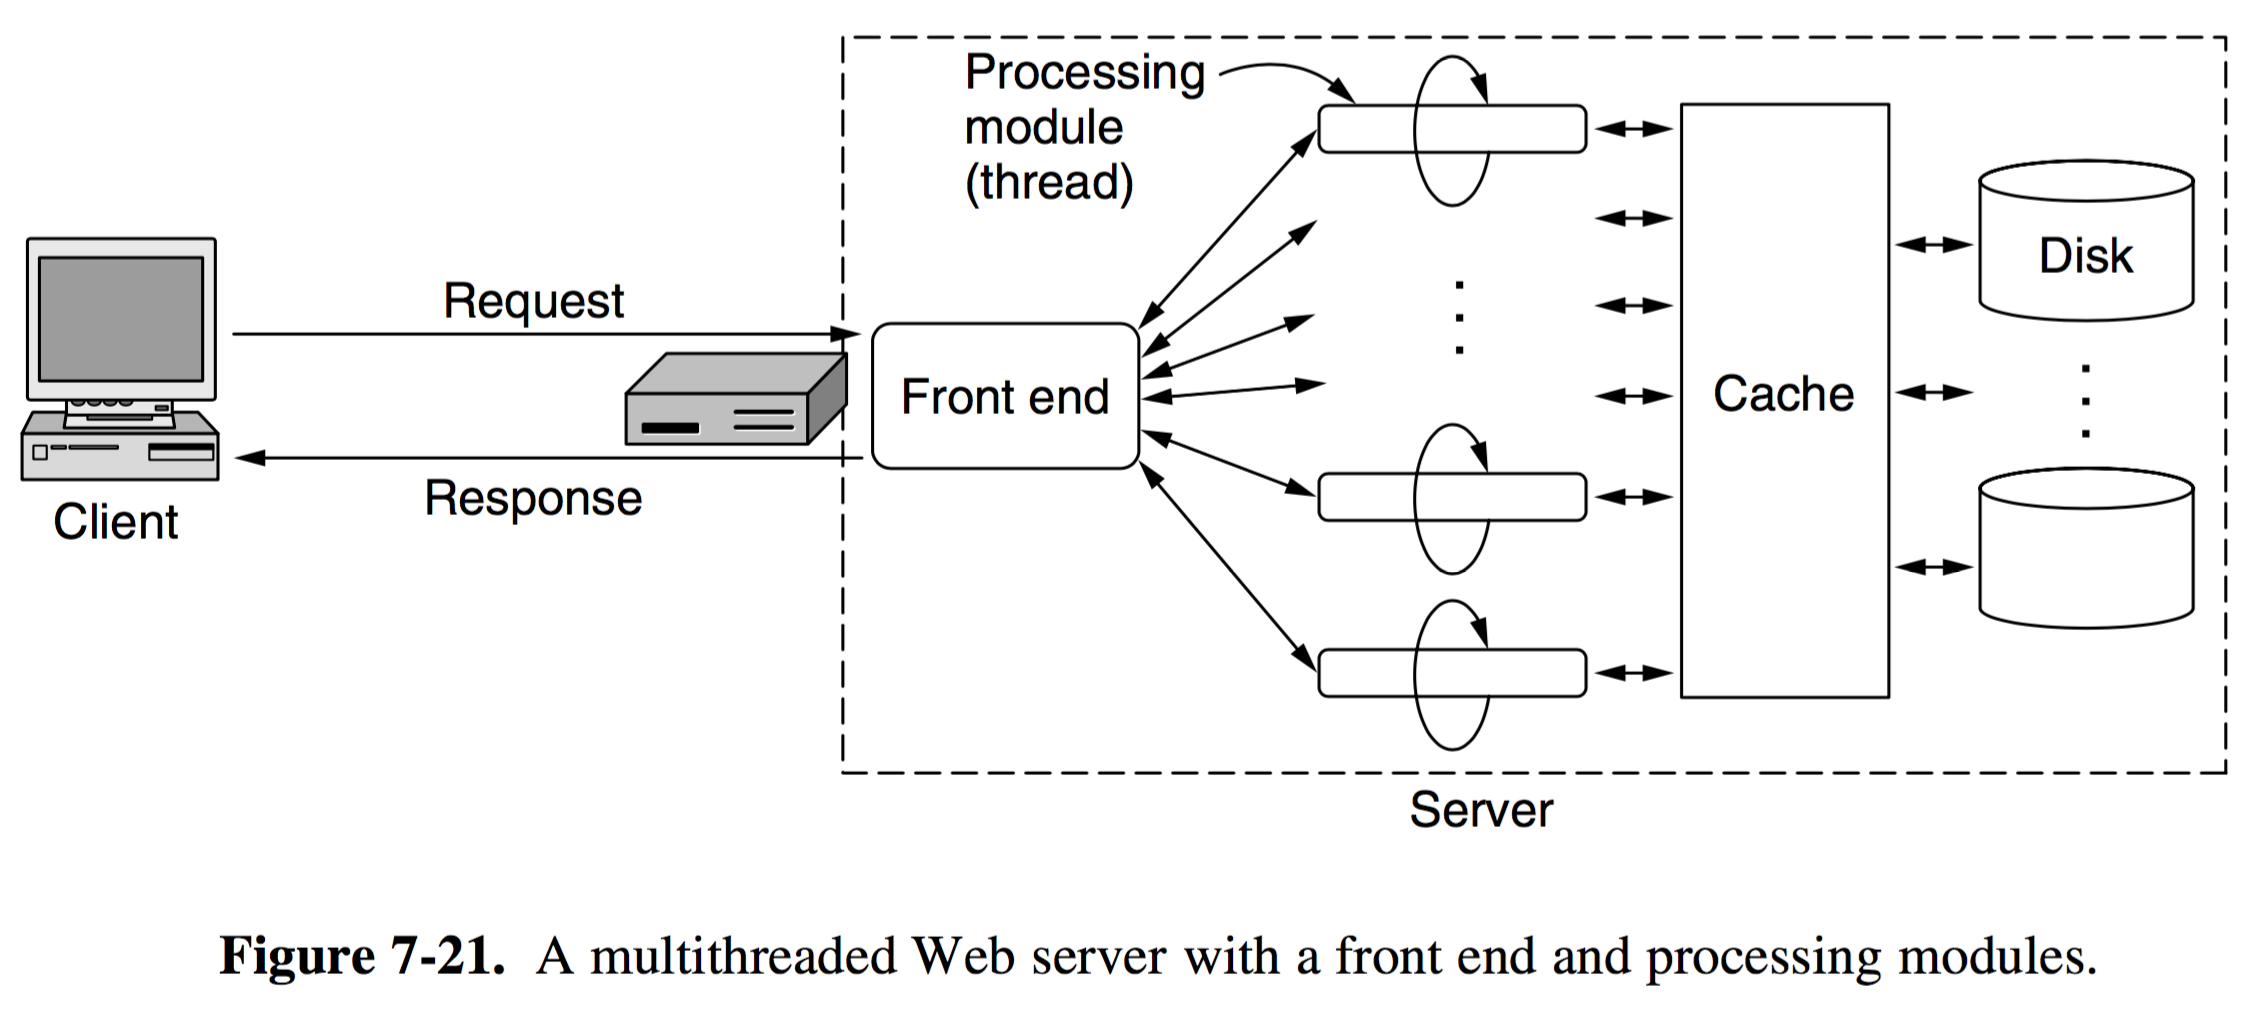
\includegraphics[width=9cm, height=5cm]{./imagenes/frontend.png} 
				\end{center}
				
				\par A continuación los pasos de un servidor web con múltiples hilos:
				
				\begin{enumerate}
					\item Cuando llega una solicitud el \textit{front-end} la acepta y construye un registro corto que la describe.
					\item Después entrega el registro a uno de los módulos de procesamiento.
					\item El módulo de procesamiento primero verifica el caché para ver si el archivo está allí.
					\item Si el archivo está en caché actualiza el registro para incluir un apuntador al archivo.
					\item Si el archivo no está en caché el módulo de procesamiento inicia una operación de disco. Cuando el archivo llega del disco se coloca en la caché y se regresa al cliente.
					\item Mientras uno o más módulo de procesamiento están bloqueados esperando a que termine una operación del disco, otros módulo de procesamiento pueden estar trabajando en otras solicitudes.
					\item Conviene tener además múltiples discos, para que más de un disco pueda estar ocupado al mismo tiempo.
				\end{enumerate}

				\par Los modernos servidores web hacen más que sólo aceptar nombres de rutas y regresar archivos. De hecho, el procesamiento real de cada solicitud puede ser muy complicado. Por esta razón, en muchos servidores cada módulo de procesamiento realiza una serie de pasos. El \textit{front-end} pasa cada solicitud entrante al primer módulo disponible, que a su vez la atiende mediante el uso de algún subconjunto de los siguientes pasos:
				
				\begin{enumerate}
					\item \textbf{Resuelve el nombre de la página web solicitada:} La solicitud entrante tal vez no contenga el nombre real del archivo como una cadena literal. Ej: se puede recibir un nombre de dominio sin nombre de archivo; este tiene que expandirse a un nombre de archivo predeterminado. Los navegadores pueden especificar el lenguaje predeterminado del usuario, lo cual posibilita que el servidor seleccione una página web en ese lenguaje.
					\item \textbf{Autentica al cliente:} se usa para las páginas que no están disponibles para el público en general.
					\item \textbf{Realiza el control de acceso en el cliente:} se verifica si hay restricciones con respecto a si la solicitud se puede satisfacer a partir de la identidad y ubicación del cliente.
					\item \textbf{Realiza el control de acceso en la página web:} Se verifica si hay restricciones de acceso asociadas con la página misma. La página deseada puede prohibir que dominios particulares accedan al archivo.
					\item \textbf{Verifica el caché}.
					\item \textbf{Obtiene del disco la página solicitada}: se necesita poder manejar múltiples lecturas de disco al mismo tiempo.
					\item \textbf{Determina el tipo MIME que se incluirá en la respuesta}: se determina el tipo MIME a partir de la extensión del archivo, de las primeras palabras del archivo, de un archivo de configuración y, posiblemente de otros recursos.
					\item \textbf{Se encarga de diversos detalles:} por ejemplo la construcción de un perfil de usuario o la recolección de ciertas estadísticas.
					\item \textbf{Regresa la respuesta al cliente}.
					\item \textbf{Realiza una entrada en el registro del servidor, para propósitos administrativos:} estos registros pueden examinarse en búsqueda de información valiosa acerca del comportamiento de los usuarios, como el orden en que acceden las páginas.
				\end{enumerate}

				\par Si llegan demasiadas solicitudes cada segundo, la CPU no será capaz de manejar la carga de procesamiento, sin importar cuántos discos se usen en paralelo. La solución es agregar más nodos, posiblemente con discos replicados (para evitar que los discos se vuelvan el siguiente cuello de botella). Esta idea lleva al modelo de granja de servidores, un \textit{fornt-end} aun acepta solicitudes entrantes pero las distribuye en múltiples CPUs. Las máquinas individuales podrán contar con múltiples subprocesos y canales como en el esquema anterior.

				\begin{center}
					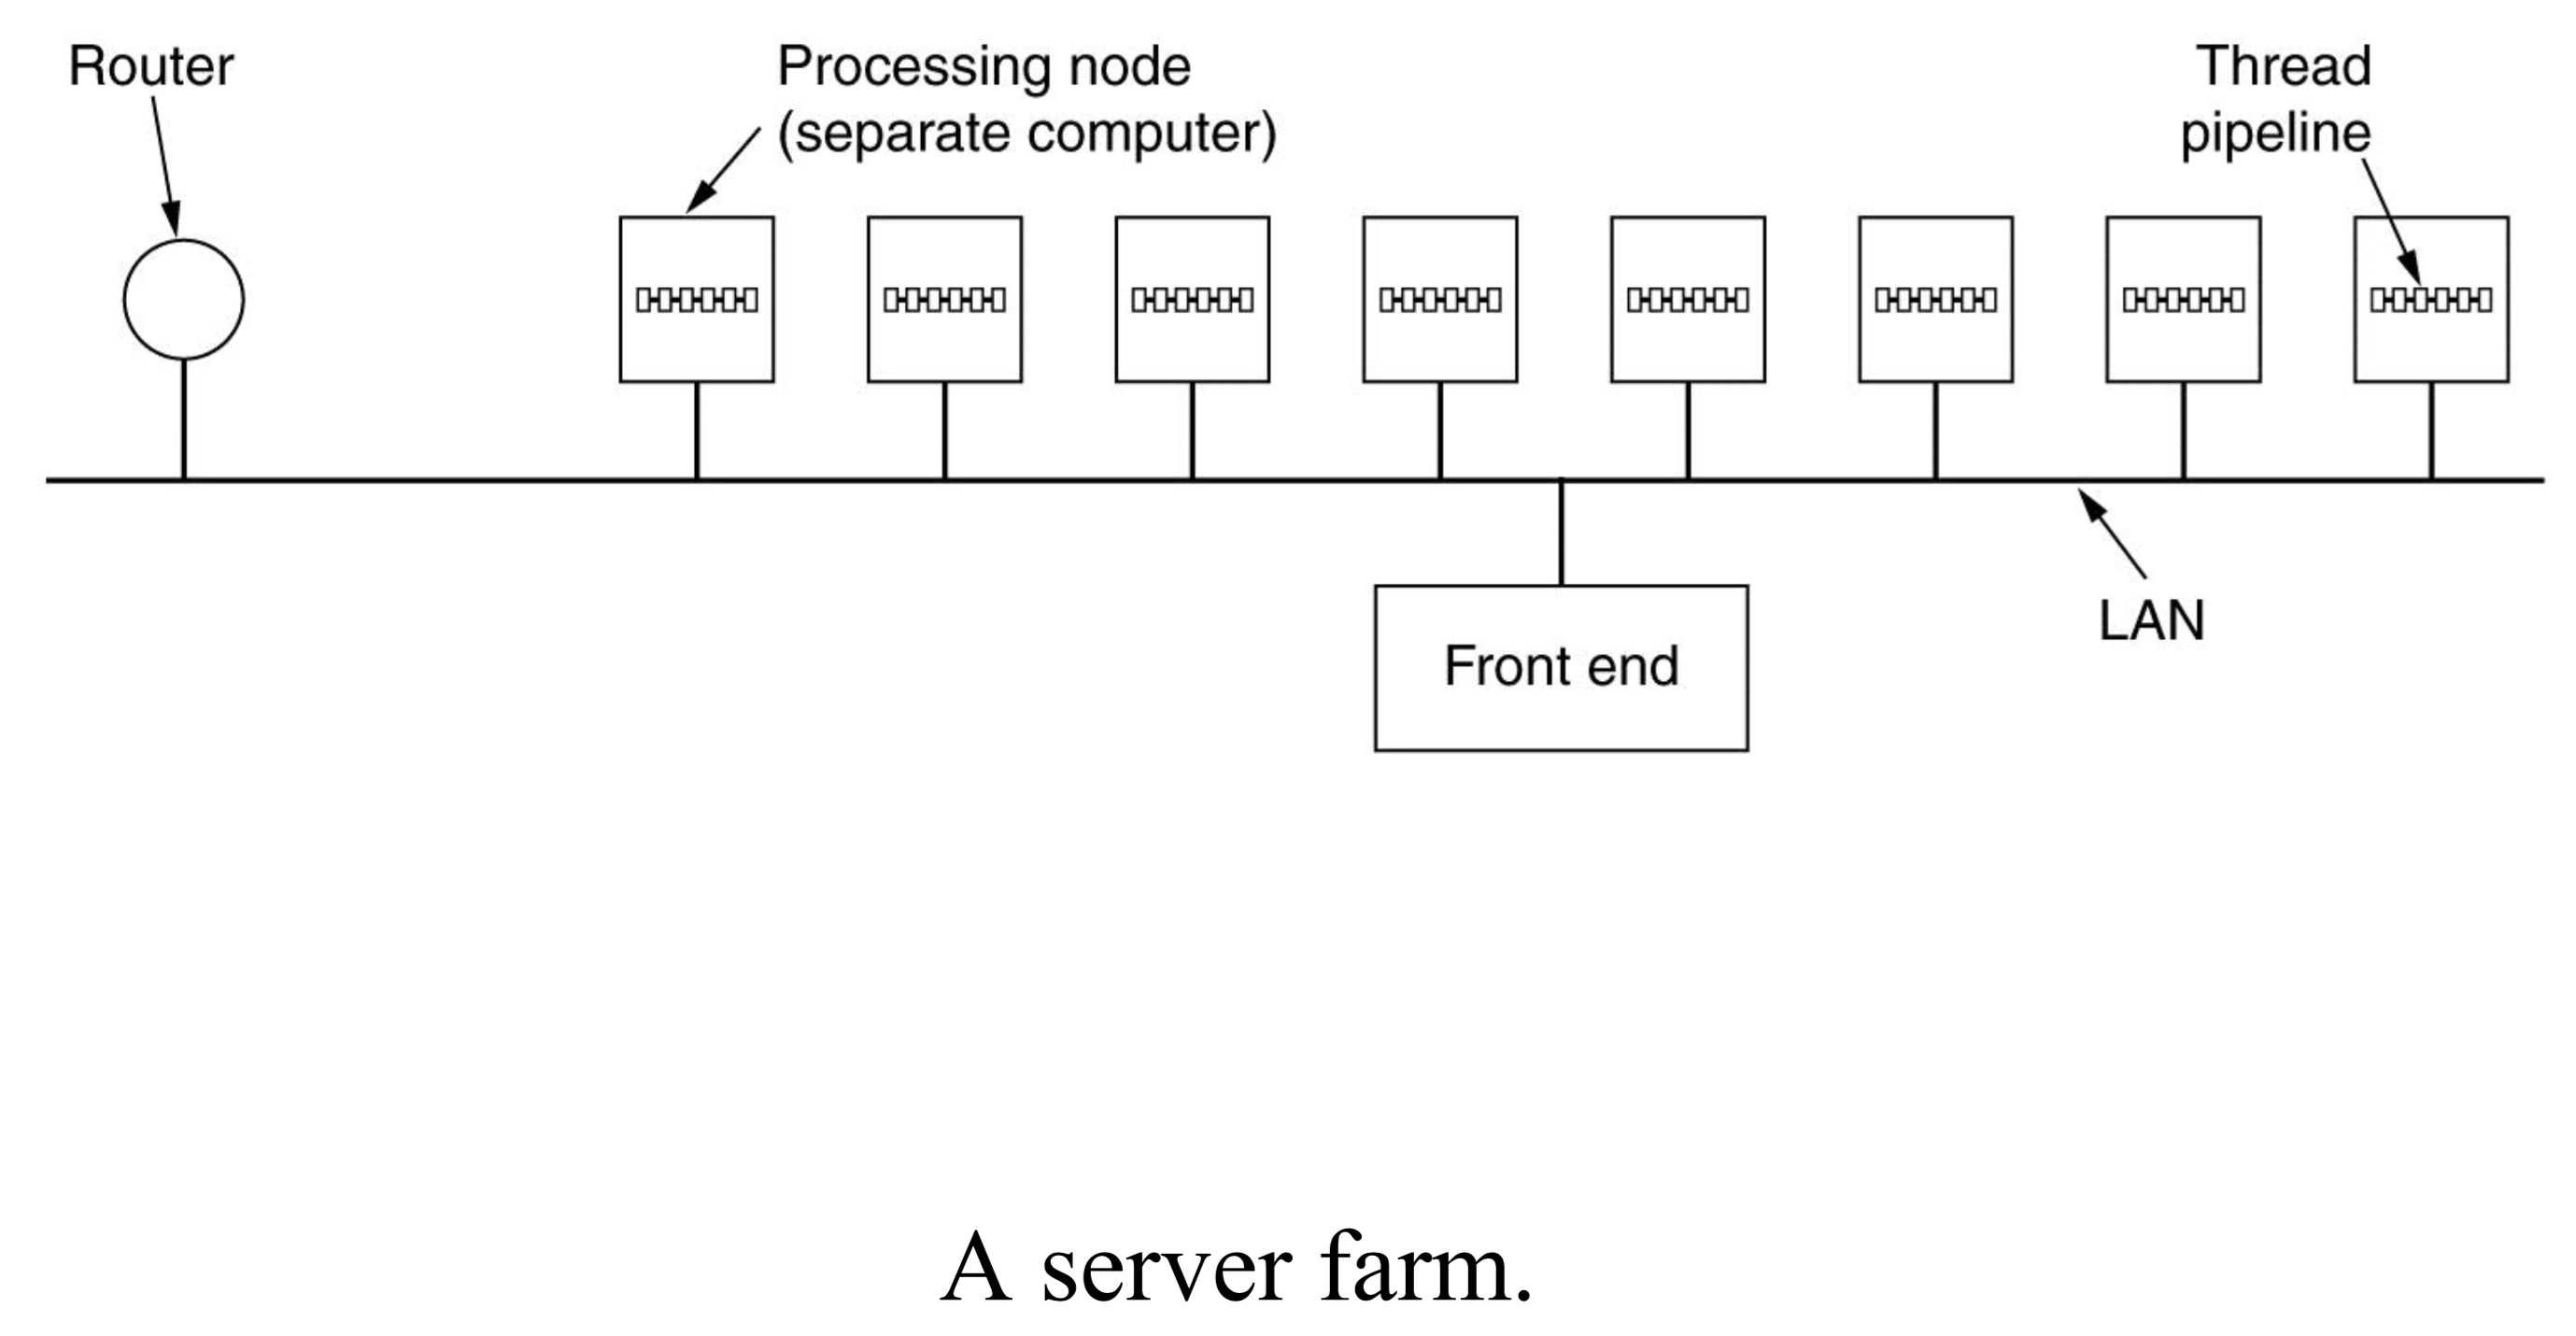
\includegraphics[width=9cm, height=5cm]{./imagenes/farm.png} 
				\end{center}

				\par En las granjas de servidores no hay caché compartido. Se puede usar un multiprocesador de memoria compartida costoso. Otra forma: Un \textit{front-end} puede registrar el lugar de donde proviene cada respuesta y enviar las solicitudes subsecuentes de la misma página al mismo nodo, así cada nodo es un especialista en ciertas páginas. Para que el espacio en caché no se desperdicie al tener cada archivo en varias caché.
				
				\par Otro problema problema es que en las granjas de servidores la conexión TCP del cliente termina en el \textit{front-end}, por lo que la respuesta pasa a través del \textit{front-end}. El punto final de la conexión TCP se pasa al nodo de procesamiento a fin de que pueda contestar directamente al cliente. Esto se llama \textbf{transferencia de TCP}.

				\begin{center}
					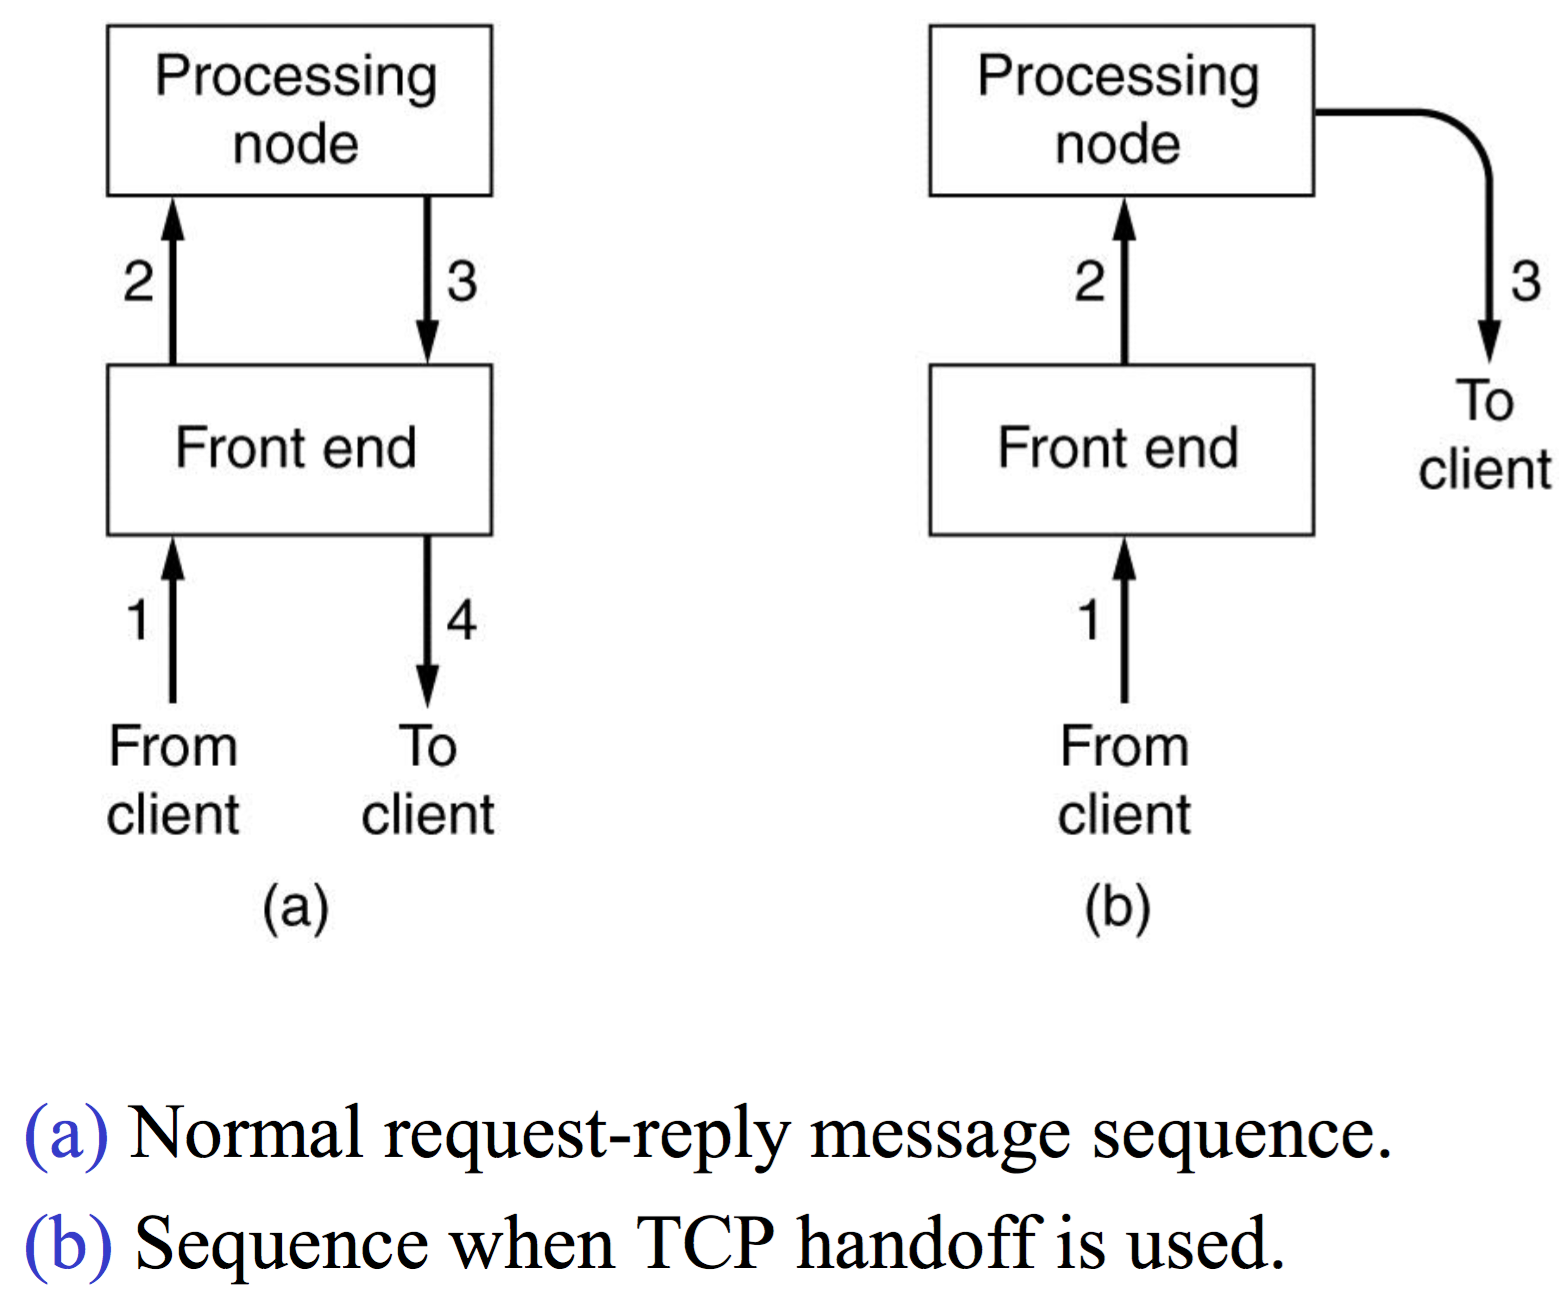
\includegraphics[width=8cm, height=5cm]{./imagenes/serverfarm.png} 
				\end{center}

			\subsubsection{Cookies}
				
				\par Luego de retornar una página web el servidor olvida que ha visto alguna vez a ese cliente particular. Algunos sitios web requieren que los usuarios se registren para poder usarlos. En comercio electrónico, si un usuario navega y coloca artículos en un carrito de compras de vez en cuando.
				
				\par Los servidores podrían seguir la pista de los usuarios al ver sus direcciones IP. Esta idea no funciona ya que hay muchos usuarios trabajando con computadoras compartidas y muchos ISP utilizan NAT por lo que todos los paquetes salientes de todos los usuarios tienen la misma dirección IP. Netscape diseñó una técnica llamada \textit{cookies}. Una cookie es un pequeño archivo o cadena (de a lo sumo 4KB). Los navegadores almacenan cookies ofrecidas en un directorio de cookies, en el disco duro de la máquina del cliente, al menos que el usuario las haya deshabilitado.

				\par Cuando un cliente solicita una página web, el servidor puede proporcionar una cookie (conteniendo información adicional) junto con la página solicitada. Justo antes de que un navegador solicite una página a un sitio web, verifica su directorio de cookies para ver si el dominio al que está solicitando la página ya colocó alguna cookie. De ser así, todas las cookies para ese dominio se incluyen en el mensaje de la solicitud. Cuando el servidor web las obtiene, puede interpretarlas de la forma que desee.

				\par Una cookie puede contener hasta 5 campos.
				
				\begin{enumerate}
						\item El \textbf{dominio} indica de dónde viene el cookie. Cada dominio puede almacenar hasta 20 cookies por cliente.
						\item La \textbf{ruta} en la estructura del directorio del servidor que identifica qué partes del árbol de archivos del servidor podrían usar el cookie.
						\item El campo \textbf{contenido} toma la forma $nombre = valor$.
						\item El campo \textbf{expira} indica cuando caduca la cookie. Si este campo está ausente, el navegador descarta la cookie cuando sale (\textit{cookies no persistentes}). Si se proporciona una hora y una fecha se dice que la cookie es persistente y se mantiene hasta que expira.
						\item El campo \textbf{seguro} puede establecerse para indicar que el navegador podría simplemente regresar la cookie a un servidor seguro. Esto se usa para aplicaciones seguras (Ej: comercio electrónico, actividades bancarias, etc.) 
				\end{enumerate}

				\begin{center}
					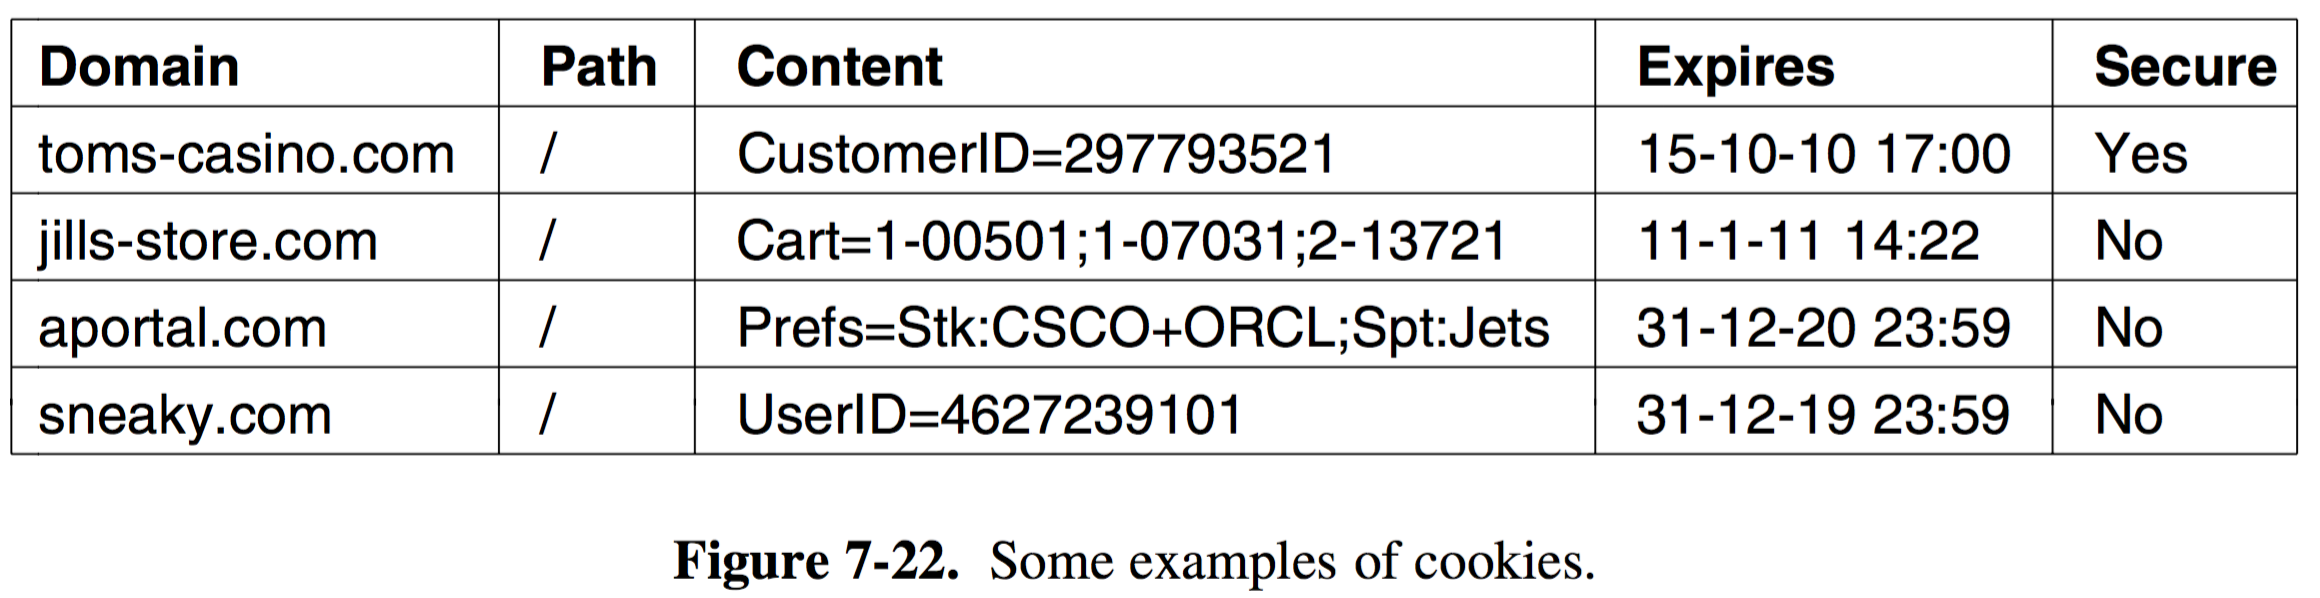
\includegraphics[width=11cm, height=4cm]{./imagenes/cookie.png} 
				\end{center}
								
				\par Para eliminar una cookie del disco duro de un cliente, el servidor simplemente la envía nuevamente, pero con una fecha caducada.



\begin{thebibliography}{X}
\bibitem{Baz} \textsc{tanenbaun andrew S. y wetherall, david j.}
\textit{Redes de Computadoras}, Quinta edición,
\textsc{pearson educación}, México, 2012.
\bibitem{Dan} \textsc{durán, juan },
<<Redes y Sistemas Distribuidos, filminas de clase>>,
\textit{FaMAF, UNC}.
\end{thebibliography}

\end{document}
